%Documento maestro.
\documentclass[a4paper,oneside,11pt]{extreport} %no funcionó tufle-book. Demasiada incompatibilidad con lo que tengo... mejor lo dejamos aspi. Original: extreport. También funciona 'article', pero no reconoce el environment de chapter.
%%%% Mis paquetes %%%%
\usepackage[utf8]{inputenc}
\usepackage{comment} %para comentar párrafos largos
						

				
\usepackage[most]{tcolorbox} %para encerrar texto en cajas de colores
\usepackage[spanish]{babel}
\decimalpoint
\usepackage{mathtools}% http://ctan.org/pkg/mathtool
\usepackage{amsthm} 


\usepackage{subcaption, threeparttable}
\usepackage{graphicx} 
\graphicspath{{./imagenes}}
\DeclareCaptionFormat{custom}
{
    \textbf{#1#2}\textit{\small #3}
}
\captionsetup{format=custom}
\usepackage[font=small,labelfont=bf]{caption} %para que los nombres 'Figura x' estén en negritas.

\usepackage{wrapfig}
\usepackage{lscape}
\usepackage{rotating}
\usepackage{epstopdf}

%Gilles C. paquetes para imagenes con Inkscape
\usepackage{import}
\usepackage{xifthen}
\usepackage{pdfpages}
\usepackage{transparent}

\newcommand{\incfig}[1]{%
    \def\svgwidth{\columnwidth}
    \import{./imagenes}{#1.pdf_tex}}

\usepackage{amsmath,bm}
\usepackage{marginnote} %Para escribir en los márgenes
\usepackage{xcolor, color, soul}
\DeclareRobustCommand{\hlAME}[2]{{\sethlcolor{#1}\hl{#2}}}

%mis colores
\definecolor{ameMorado}{HTML}{816780}
\definecolor{ameDorado}{HTML}{e4bc8c}
\definecolor{ameRosa}{HTML}{FF69B4}
\definecolor{ameAzul}{HTML}{41BBE0}

\usepackage{tikz}
\usepackage[toc,page]{appendix}  
\usepackage{enumerate}
\usepackage{lscape} %Para tablas horizontales.
\usepackage{verbatim}


\usepackage{natbib}
%\usepackage{chngcntr}
%\counterwithin{equation}{section}


%Para escribir pseudocódigo
\usepackage{algorithm}
\usepackage{algorithmic}
\renewcommand{\algorithmicrequire}{\textbf{Input:}}
\renewcommand{\algorithmicensure}{\textbf{Output:}}
\newcommand{\code}[1]{\texttt{#1}}
%\swapnumbers %Para tener un solo contador para TODOS los 'equation' environment.

\usepackage{amssymb}
\usepackage{mdframed} %Símbolos en cajas
\usepackage{amsmath} %it is best to load this package if doing any serious mathematical layout with LaTeX
\usepackage{cases}
\usepackage{bm} %Bold math text
\usepackage{marvosym}
\usepackage{fancyref}
\usepackage{graphicx}
\usepackage{float}
\usepackage{graphicx}
\usepackage{blindtext}
\usepackage{titlesec}
\usepackage{imakeidx}
\usepackage{scalerel}

%Paquetes usados en estilo.tex
\usepackage{geometry}
\usepackage{sidenotes} 
\usepackage[font=footnotesize,format=plain,labelfont={bf,sf},textfont={it},width=10pt]{caption}
% Captions at the side of the page
%\usepackage[wide]{sidecap}
\usepackage{morefloats}
\usepackage{marginfix}

\usepackage{hyperref}
\usepackage{subfiles} % Best loaded last in the preamble

%%%% Mis macros %%%%

			%% Secciones:
			%Pongo a todas el contador de 'teo'
			\newtheorem{teo}{Teorema}[section]
			\newtheorem{lema}[teo]{Lema}
			\newtheorem{prop}[teo]{Proposición}
			\newtheorem{obs}[teo]{Observación}
			%\newtheorem{dem}[teo]{Demostración}
			\newtheorem{cor}[teo]{Corolario}
			\newtheorem{defi}[teo]{Definición}
			\newtheorem{ej}[teo]{Ejemplo}
			\newtheorem{notacion}[teo]{Notación}
			\newtheorem{listaObj}[teo]{Lista de objetivos}
			
			%\theoremstyle{definition}
			\newtheorem{nota}[teo]{Nota}
			%\newtheorem{teo}[equation]{\textbf{Lema}}
			%\newtheorem{lema}[equation]{\textbf{Lema}}
			%\newtheorem{prop}[equation]{\bf Proposición}
			%\newtheorem{obs}[equation]{\bf Observación}
			%\newtheorem{dem}[equation]{\bf Demostración}
			%\newtheorem{cor}[equation]{\bf Corolario}
			%\newtheorem{defi}[equation]{\bf Definición}
			%\newtheorem{ej}[equation]{\bf Ejemplo}
			%\newtheorem{notacion}[equation]{\bf Notación}

			
			%\theoremstyle{definition}
			%\newtheorem{nota}[equation]{\bf Nota}

			%% Símbolos matemáticos
			
			\newcommand{\demostracion}{\textbf{Demostración.} \hspace*{0.1cm}}
			\newcommand*{\QEDA}{\null\nobreak\hfill\ensuremath{\blacksquare}}%
			\newcommand*{\QEDB}{\null\nobreak\hfill\ensuremath{\square}}%
			
			\newcommand{\TODO}[1]{\textcolor{purple}{#1}}
			\newcommand{\bien}[1]{\textcolor{blue}{Revisado.}}
			
			\newcommand*{\final}{\null\nobreak\hfill\ensuremath{\diamond}}
			\newcommand{\IR}{\mathbb{R}}
			\newcommand{\IC}{\mathbb{C}}
			\newcommand{\IN}{\mathbb{N}}
			\newcommand{\IP}{\mathbb{P}}
			\newcommand{\IZ}{\mathbb{Z}}

			\newcommand{\La}{\Lambda}			
			
			\newcommand{\suma}[3]{\sum\limits_{#1}^{#2}#3} %Sumas y series
			\newcommand{\union}[3]{\bigcup\limits_{#1}^{#2}{#3}} %uniones
			\newcommand{\producto}[3]{\prod_{#1}^{#2}{#3}} %productos
			\newcommand{\limite}[2]{\lim\limits_{#1}{#2}} %límites
			\newcommand{\limsu}[2]{\lim\limits_{#1 \rightarrow \infty }#2_{#1}}
			%para límites de sucesiones
			\newcommand{\Om}{\Omega}
			\newcommand{\cali}[1]{\mathcal{#1}} %Letras caligráficas
			\newcommand{\cont}[2]{$\mathcal{C} [#1, #2]$}
			\newcommand{\integ}[3]{\int_{#1}^{#2}{#3}}
			\newcommand{\ldos}{\mathit{l}^{2}}


			\DeclareMathOperator*{\ameboxplus}{{\boxplus}}



%macros Moisés
\newcommand{\aplica}[5]{\text{${\begin{array}{crcl} #1: & #2 & \longrightarrow & #3 \\ \, & #4 & \longmapsto & #5 \end{array}}$}} %Notación para la definición de una aplicación.
\newcommand{\demo}[1]{\textbf{Demostración:} #1 \nopagebreak[4] $\square$ \\}
			
			
%Source: https://tex.stackexchange.com/questions/68010/how-to-create-multilevel-colored-boxes-using-tcolorbox-any-other-package
\makeatletter
\newcommand{\DrawLine}{%
  \begin{tikzpicture}
  \path[use as bounding box] (0,0) -- (\linewidth,0);
  \draw[color=black,dashed,dash phase=2pt]
        (0-\kvtcb@leftlower-\kvtcb@boxsep,0)--
        (\linewidth+\kvtcb@rightlower+\kvtcb@boxsep,0);
  \end{tikzpicture}%
  }
\makeatother




%%%% Datos generales del archivo %%%%
\title{Tesis}
\author{Amélie Bernès}

%Estilo de página. Tengo una pequeña columna vertical, en la que agrego imágenes, nota, texto... lo que quiera.
%Gilles Castel.

\captionsetup{font=footnotesize, skip=4pt}

\geometry{
paperwidth=210mm,
paperheight=297mm,
left=72pt,
top=42pt,
textwidth=360pt,
marginparsep=20pt,
marginparwidth=110pt,
textheight=650pt,
footskip=40pt,
}



\renewcommand{\normalsize}{\fontsize{10pt}{13pt}\selectfont}%
\renewcommand{\footnotesize}{\fontsize{8pt}{10pt}\selectfont}%
% fullwidth environment, text across textwidth+marginparsep+marginparwidth
\newlength{\overhang}
\setlength{\overhang}{\marginparwidth}
\addtolength{\overhang}{\marginparsep}
%
\newenvironment{fullwidth}
  {\ifthenelse{\boolean{@twoside}}%
     {\begin{adjustwidth*}{}{-\overhang}}%
     {\begin{adjustwidth}{}{-\overhang}}%
  }%
  {\ifthenelse{\boolean{@twoside}}%
    {\end{adjustwidth*}}%
    {\end{adjustwidth}}%
  }


\makeindex
\begin{document}
%Portada. 

\thispagestyle{empty} %para no tener número en esta página

\begin{center}
{\Large{
\textsc{Benemérita Universidad Autónoma de Puebla}
}} \\
\vspace{0.5cm}
{\Large{
\textsc{Facultad de Ciencias Físico Matemáticas}
}}
\end{center}


\begin{figure}[H]
	\centering
	
\includegraphics[scale=0.35]{logo_buap} 
\end{figure}	



\hrule
\vspace{0.5cm}
\begin{center}
{\Large {Estudio y análisis espectral de los polinomios \\
discretos de Legendre}}
\end{center}
\vspace{0.5cm}
\hrule


\begin{marginfigure}
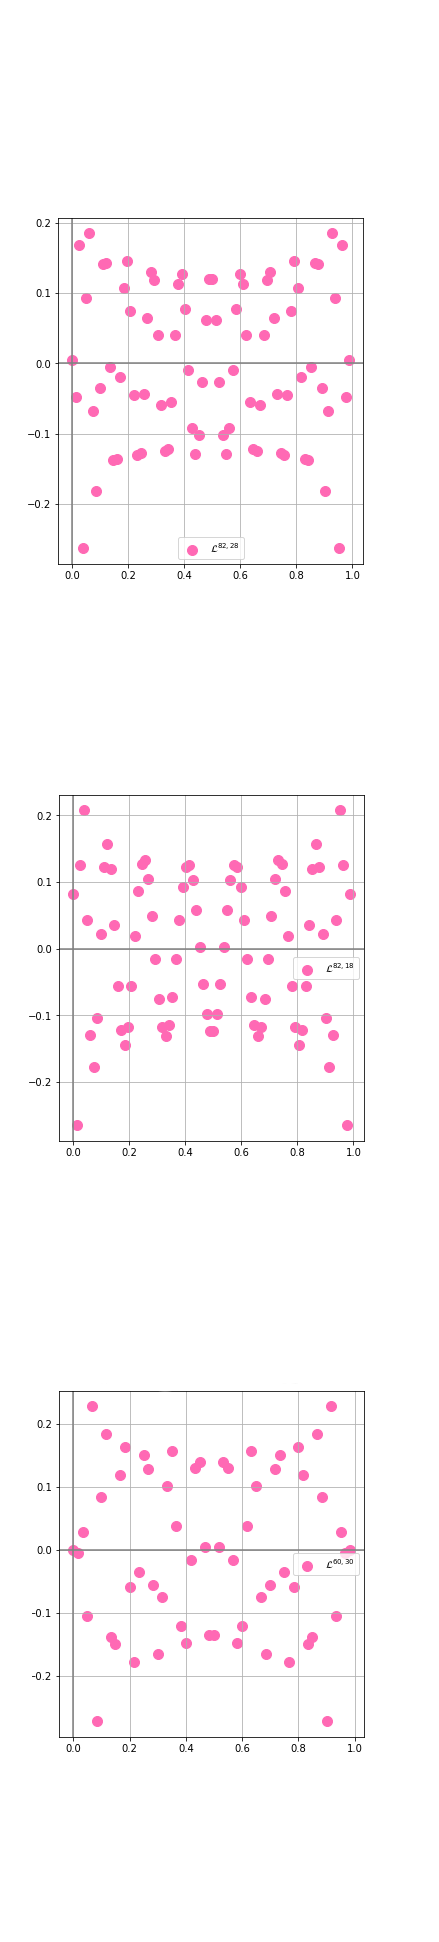
\includegraphics[scale=1.3]{portada_tesis2} 
\end{marginfigure}






\vspace{4cm}

\noindent
\textsc{Tesis} \\
que para obtener el grado de \\
\textsc{licenciada en matemáticas} \\
presenta \\
\textsc{Denisse Amélie Sophie Bernès Carmona}



\vspace{2cm}

\noindent
Asesor: \textsc{Dr. Moisés Soto Bajo} \\
Co-asesor: \textsc{Dr. Javier Herrera Vega} 




\vspace*{\fill}
Puebla, Pue. Junio del 2023 







%Texto usado para la imagen lateral. 
%\textsc{Dimensión $n$}\\
%\vspace{1cm}
%\underline{\textsc{Señales constantes, $W_{n,0}$.}}\\
%\vspace{1cm}
%\underline{\textsc{Señales afines, $W_{n,1}$.}}\\
%\vspace{1cm}
%\underline{\textsc{Señales cuadráticas, $W_{n,2}$.}}\\
%\vspace{1cm}
%\underline{\textsc{Señales $n$-dimensionales, $W_{n,n-1}$.}} \\
%\vspace{1cm}
%$\vdots$

%\vspace{5cm}

\newpage
%Agradecimientos--------------------
\thispagestyle{empty} %para no tener número en esta página


\vspace*{\fill}
\begingroup
\centering

Gracias

\begin{itemize}
\item al Dr. Moisés Soto Bajo, por 
la gran oportunidad que me brindó al permitirme trabajar
bajo su tutela,
por brindarme su tiempo, apoyo y confianza durante todo el proceso,
y por ser un ejemplo a seguir,

\item a mi co-asesor, el Dr. Javier Herrera Vega, por 
la ayuda brindada para la realización de la parte 
computacional de este trabajo,

\item a mis sinodales, el
Dr. Andrés Fraguela Collar, 
el Dr. Jorge Bustamante González
y la Dra. Alina Santillán Guzmán, por 
el valioso tiempo dedicado
para leer y comentar este trabajo, 

\item a todos los que comparten libremente
el conocimiento (y a los que permiten encontrarlo),

\item a mi familia, por todo.
\end{itemize} 

\endgroup
\vspace*{\fill}


\newpage
\thispagestyle{empty}
\vspace*{\fill}
\begingroup


\textit{
—Ves, Momo —le decía, por ejemplo—, las cosas son así: a veces tienes ante ti una calle larguísima. Te parece tan terriblemente larga, que nunca crees que podrás acabarla.} \\

\textit{ 
Miró un rato en silencio a su alrededor; entonces siguió:} \\

\textit{ 
—Y entonces te empiezas a dar prisa, cada vez más prisa. Cada vez que levantas la vista, ves que la calle no se hace más corta. Y te esfuerzas más todavía, empiezas a tener miedo, al final estás sin aliento. Y la calle sigue estando por delante. Así no se debe hacer.}\\

\textit{ 
Pensó durante un rato. Entonces siguió hablando:} \\

\textit{ 
—Nunca se ha de pensar en toda la calle de una vez, ¿entiendes? Sólo hay que pensar en el paso siguiente, en la inspiración siguiente, en la siguiente barrida. Nunca nada más que en el siguiente.} \\

\textit{ 
Volvió a callar y reflexionar, antes de añadir:} \\

\textit{ 
—Entonces es divertido; eso es importante, porque entonces se hace bien la tarea. Y así ha de ser.} \\

\textit{ 
Después de una nueva y larga interrupción, siguió:}\\

\textit{ 
—De repente se da uno cuenta de que, paso a paso, se ha barrido toda la calle. Uno no se da cuenta cómo ha sido, y no se está sin aliento.}\\

\textit{ 
Asintió en silencio y dijo, poniendo punto final:}\\

\textit{ 
—Eso es importante.}

\null\hfill \textbf{Michael Ende}\\
\null\hfill Momo

\endgroup
\vspace*{\fill}
\textbf{23 Noviembre- Pendientes}
\begin{itemize}

\item \TODO{Cambia las figuras. Fija un color
	(rosa) para TODAS
	las gráficas de señales $x$.}.

\item \textbf{revisar literatura}
\item \textbf{implementar en python los polinomios discretos de Lendre}: Listo!
Ahora debería de intentar usar algunas librerías que encontré
sobre polinomios discretos de Legendre.

\item hacer un mapa sobre cómo se relacionan unos
resultados con otros.
\item \textbf{Dimensión, grado, posición.}
\item Cambia todos los entornos de demostración

\item revisa que siempre digas que la dimensión
del polinomio discreto es $n$.

\item ¿Deberían adjuntar en la tesis una copia de Survey?Porque
cito muchas veces fórmulas de ahí.  

\item \textbf{SÍ es importante poner la dependencia a $n$ de los espacios
$W_{k}$. Es muy confuso si no lo haces así.}

\item cambia el formato de las captions para figuras.

\item revisa que usas $t_{i}$ y no $x_{i}$ para puntos
de la malla.

\item nemu

\item Deberías ver este video:  \url{https://www.youtube.com/watch?v=q5Nsc4LyhdE&ab_channel=SeminarioGAMMA}

\item poner macadores para el final de un ejemplo.

\item Cambiar comas por puntos en el entorno align. Creo que
esto se corrige si pones la cita dentro de un entorno
de texto.

\item marcador al final de ejemplos. \final

\item Cambia los símbolos <,> por langle y rangle.

\item Preguntar al Dr. Gabriel por información.

\item ve cuándo es la primera vez que citas en TFA y da la
formulación dada en rotman.

\item Di que algunos autores dicen que el grado del polinomio
cero no está definido, pero para nosotros es cero.

\item checa que las discretizaciones de los de legendre no son
los que tengo yo.

\end{itemize}

\newpage
 

%--- Disclaimer.


\begin{abstract}

Motivados por la busqueda de un sistema
de representación de $\IR^{n}$ adecuado para
el estudio morfológico de señales finitas
(c.f. lista de deseos \ref{lista de objetivos}), 
para cada $n \in \IN$ mayor a uno, definimos
(c.f. capítulo \ref{cap: def y propiedades de los pol discretos de Legendre}) 
$n$ vectores de $\IR^{n}$, que llamamos
\textbf{polinomios discretos de Legendre} (aka PDL),
cada uno asociado a un grado entero $k$ de $0$ a $n-1$,
que juntos conforman una base ortonormal de $\IR^{n}$,
la \textbf{base de Legendre discreta $n-$dimensional} y que, 
como mostramos (c.f. capítulo \ref{sec: ejemplos}), 
cumple satisfactoriamente nuestros requisitos.\\

Encontramos en la literatura que estos objetos ya se habían 
definido antes
(c.f. \cite{Neuman}), pero no encontramos una construcción
rigurosa de estos como la dada por nosotros ni
aplicaciones de los PDL para estudios de morfología. \\

Hacemos también un estudio de simetrías de los PDL 
(c.f. capítulo \ref{section: sobre simetrias en las entradas de los poliomios discretos de Legendre})
que, junto con las fórmulas dadas en \cite{Neuman}, 
será usado para definir algoritmos 
(c.f. capítulo \ref{Implementación computacional de las bases discretas de Legendre en Python})
para programar a los PDL de cualquier dimensión $n$.
Las implementaciones en Python pueden encontrarse en el repositorio
\TODO{ref.}\\

Se realizó además un análisis espectral de los PDL
(c.f. capítulo \ref{chap: estudio espectral})
que nos llevó
a plantear una interesante conjetura en la que establecemos
una relación (que depende sólo de los parámetros de dimensión
$n$ y grado $k$) entre frecuencias y polinomios discretos de Legendre
\TODO{explica mejor esto.}.\\


Para que los conceptos y herramientas que usamos a lo largo
del desarrollo de este trabajo queden claras, incluimos al final
un apéndice de teoría en el que
plasmamos algunos resultados o definiciones que son estrictamente
necesarios para el desarrollo de este trabajo de tesis.
Preferimos no limitarnos a citar referencias que abordaran estos temas,
pues definiciones presentes en unas son diferentes a las usadas por otras;
además, para algunos resultados clásicos (como el teorema de Gram-Schmidt)
necesitabamos dar formulaciones distintas a las canónicas pero útiles para
nosotros.\\


Mostrada con teoría y ejemplos  cómo las
bases de Legendre discretas
son un sistema de representación particularmente útil
para hacer un estudio cuantitivo de morfología
(y, potencialmente, un análisis espectral también)
de señales finitas, esbozamos cómo esto da lugar a
trabajos a futuro en esta línea.\\

\mbox{}
\vfill
Este trabajo fue escrito en \LaTeX.
El lenguaje de programación de nuestra elección
para el desarrollo de la parte computacional 
fue Python.
La mayoría de las imágenes aquí presentadas fueron,
a su vez, programadas en Python y, en algunas ocasiones,
retocadas (o dibujadas completamente) en Krita. 
El formato adoptado 
se basa en el diseño de los libros de 
Edward Tufte.
\end{abstract}



%--Índice
\tableofcontents
\newpage 
%-- Cuerpo
%- Nota: prefiero no anidar los archivos .tex en carpetas,
% sino en archivos:) por ejemplo, los input de este .tex
% tiene sólamente inputs; en esos inputs está todo el escrito.
% Así que puedes pensar a los input de este archivo como carpetas.



%%\thispagestyle{empty}
%\vspace{13cm}
%\begin{flushright}
%{\Huge{\textbf{Parte I}}}
%\label{ParteI header}

%\TODO{aquí un resumen de lo que se hace en esta parte de la tesis.}
%\end{flushright}

%\clearpage


\chapter{Definición y propiedades de los polinomios discretos de Legendre}
\label{cap: def y propiedades de los pol discretos de Legendre}
\label{cap: def de los pol de legendre discretos}

\section{Introducción: planteamiento y motivación}
Durante todo este trabajo trataremos con señales
finitas
(digamos, de
longitud $n$), y las pensaremos como elementos de $\IR^{n}$.
En la práctica, por lo general
una señal es un conjunto de mediciones tomadas
a intervalos regulares de tiempo.
Puesto que por el momento no vamos
a considerar la localización temporal, dicha
información perfectamente puede expresarse como 
una $n-$tupla. En lo que sigue, a menos que se diga
lo contrario, usaremos indistíntamente los nombres
``vector'' y ``señal'.'

Es costumbre empezar
a enumerar las entradas de un vector
de $x \in \IR^{n}$ a partir de uno, pero
para nuestros fines,
como se verá más adelante, es más 
conveniente empezar desde el cero.
Adoptamos pues esta convención.

\sidenote{\TODO{Di por qué prefieres
evitar el nombre ``'lineal'. Baja la nota a
la altura de la def.}}

\begin{defi}
\label{def: grafica senial}
Por la \textbf{gráfica de una señal} $x=(x_{j})_{j=0}^{n-1}$
de dimensión $n$ entenderemos
 el siguiente subconjunto de $\IR^{2}$:
\[
G_{x} := 
\{ (j, x_{j} ) : \hspace{0.1cm} 0 \leq j \leq n-1
\hspace{0.2cm} \text{entero}\} .
\]
Si $G_{x}$ está contenida en la gráfica de una recta, diremos que la
señal es \textbf{afín}
(en el caso particular en el que
la ecuación de la recta en cuestión sea de la forma $y= h$
(con $h$ una constante),
diremos que la señal es
\textbf{constante}). Si  $G_{x}$ está contenida en 
una parábola, o sea, en una
gráfica de ecuación cartesiana
$y=ax^{2}+ bx +c$, donde $a \neq 0$, diremos 
que la señal es \textbf{cuadrática}.
\end{defi}


\begin{figure}[H]
	\sidecaption{En la figura se pintan las gráficas
	de dos señales de dimensión 30. La gráfica de cruces 
	(resp. la de puntos)
	sugiere la forma de una recta (resp. una parábola).
	Tomamos a las formas de una parábola como cánones
	de curvas (y no, por ejemplo, trozos de circunferencias)
	sólo porque son buenos ejemplos de curvas con una sola 
	convexidad.}
	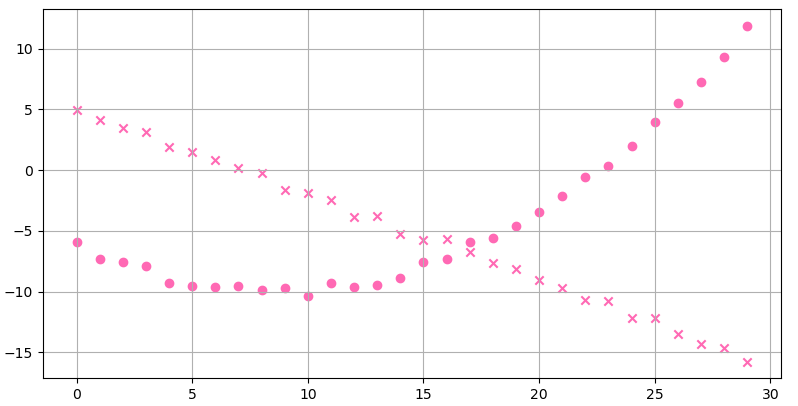
\includegraphics[scale=0.6]{ejemplo_intro} 
 \end{figure}

Puesto que el espacio subyacente de 
la teoría es el $\IR-$espacio vectorial 
$\IR^{n}$, tenemos la ventaja de contar con
bases (subconjuntos de $\IR^{n}$ linealmente
independientes y generadores de todo el espacio),
que pensamos en este contexto como sistemas
de representación: si 
\begin{equation}
\label{eq0: 13Feb}
\cali{B}=\{v_{k}
 \hspace{0.1cm} |
\hspace{0.1cm} 0 \leq k \leq n-1 \} 
\subseteq \IR^{n}
\end{equation}
es base del espacio, entonces, dado $x \in \IR^{n}$, 
\textbf{existe} \textbf{únicos} escalares
$a_{k} \in \IR$, con $0 \leq k \leq n-1$
tales que

\begin{equation}
\label{eq1: 13Feb}
x = \suma{k=0}{n-1}{a_{k}v_{k}};
\end{equation}
observe entonces que $x$ 
queda completamente determinado por los
números $a_{k}$. Si lo que nos interesa es
la forma de la gráfica de $x$, es natural preguntarse lo siguiente:

\begin{preg}
\label{preg: sist repr}
Si $\cali{B}$ es como en \eqref{eq0: 13Feb}, $x \in \IR^{n}$
y $a_{k}$ con $0 \leq k \leq n-1$ son como en 
\eqref{eq1: 13Feb}, ¿es posible establecer condiciones
necesarias y suficientes que deban cumplir los coeficientes
$a_{k}$ para que $x$ sea constante, afín o cuadrática?
\end{preg}

Después de un poco de reflexión, se llega a que la respuesta 
a la pregunta \ref{preg: sist repr} depende de la base
$\cali{B}$, y que por lo general la respuesta es negativa.
Observe además que, en la formulación de la pregunta,
se supone que para una señal $x$ se pudo dar
explícitamente a los coeficientes $a_{k}$ aunque,
en realidad,  esta es una suposición optimista.
A pesar de que la existencia y unicidad de tales
coeficientes está asegurada, el calcularlos
puede requerir el tener que resolver sistemas cuadrados
de ecuaciones con una cantidad de parámetros que
depende linealmente de $n$, sistemas que son computacionalmente
difíciles de resolver si $n$ es ``grande''.

\TODO{Poner algunos ejemplos}. Esto motiva la
creación de la siguiente lista de deseos.


\noindent 
\begin{listaObj}
\label{lista de objetivos}
Fijada una dimensión $n$, 
buscamos una base 
\begin{equation}
\label{eq1: 28Nov}
\cali{L}^{n}=\{ \cali{L}^{n,k} \hspace{0.1cm} |
\hspace{0.1cm} 0 \leq k \leq n-1  \} \subseteq \IR^{n} 
\end{equation}
del espacio vectorial
$\IR^{n}$ ``adecuada'' para la representación de señales
$x \in \IR^{n}$,
en el sentido que satisfaga
las siguientes condiciones: 

\begin{enumerate}
\item 
que
sea ortonormal, para poder hacer uso de todas
las bondades que conlleva 
trabajar con tales bases, 
bondades entre las que se encuentran
las que a continuación citamos.
\begin{itemize}
\item 
\textbf{\color{ameMorado}{(Los coeficientes de $x$ respecto
a $\cali{B}$ son muy fáciles de calcular, ...)}}
El poder no sólo dar explícitamente los coeficientes
de un vector respecto a la base, 
	\marginnote{Si $x \in \IR^{n}$ y $\cali{L}^{n}$ como en 
	\eqref{eq1: 28Nov} es BON de $\IR^{n}$, entonces identificamos a
	$x$ con los $n$ números  
	$a_{k}:= \langle x, \cali{L}^{n,k} \rangle$,
	$0 \leq k \leq n-1$.}
sino poder calcular a estos
de forma relativamente sencilla (a saber, vía productos punto,
c.f. \TODO{referencia del apéndice} ); si
\eqref{eq1: 28Nov} es ortonormal, entonces

\begin{equation}
\label{eq2: 13Feb}
x= \suma{k=0}{n-1}{a_{k}\cali{L}^{n,k}},
\hspace{0.2cm} \text{ donde } \hspace{0.2cm}
a_{k}= \langle x , \cali{L}^{n,k} \rangle.
\end{equation}
\item
\textbf{\textcolor{ameMorado}{(... dan información sobre el tamaño (norma) de $x$...)}}
El tener disponible una igualdad de tipo Parseval
(c.f. \TODO{referencia del apéndice}), igualdad que
relaciona de manera sencilla (de hecho, lineal)
el cuadrado de
la magnitud de una señal $x \in \IR^{n}$ (magnitud dada
gracias al producto punto definido en $\IR^{n}$)
con el cuadrado de las magnitudes de sus coeficientes
respecto a la base;

\[
||x||^{2}= \suma{k=0}{n-1}{|a_{k}|^{2}}.
\]

Esto es útil al momento
de intentar determinar
(de forma intuitiva) 
	\marginnote{
		Si $x':= \suma{k=0, }{n-1}{a_{k} \cali{L}^{n,k}}$
	y $|a_{i}|$ es un número ``cercano a cero'', entonces
	$||x '|| \approx ||x||$. Pensando en la norma de $x$ como
	la cantidad de información que tenía, parafraseamos esto
	como ``quitar coeficientes pequeños no hace que se
	pierda mucha información''	
	.}
la importancia 
de cierto vector de la base para describir a $x$.
También es bueno contar con esta igualdad
al momento de hacer procesos de síntesis,
es decir, de modificación de la señal
via cambios en sus coeficientes respecto
a un sistema de representación; si un coeficiente
$a_{k}$ es pequeño en magnitud, retirando el sumando
$a_{k} \cali{L}^{n,k}$ de \eqref{eq2: 13Feb}, 
estamos seguros de obtener
un vector $x'$ similar al vector original $x$
en magnitud.
\end{itemize}
\item \textbf{
\textcolor{ameMorado}{(...y sobre la forma de la
gráfica de $x$.)}} El que,
dada la expresión \eqref{eq2: 13Feb},
sea posible establecer
una relación sencilla entre \textbf{los coeficientes }
$a_{k}$
(en base a su tamaño y signo) y
\textbf{la forma de la gráfica de la señal}.
En particular, nos gustaría encontrar condiciones
necesarias y suficientes 
en términos de los coeficientes $a_{k}$ para determinar
si la gráfica de $x$ es afín o cuadrática.
Queremos pues que los coeficientes $a_{k}$
\textit{reflejen atributos geométricos de $x$};
de esta forma, 
\textbf{con herramientas del álgebra lineal lograremos cuantificar
la propiedad geométrica intuitiva de ``parecerse a''
una recta o una parábola.}
\end{enumerate} 

\end{listaObj}


\begin{comment}
Nuestro acercamiento es como sigue:
\end{comment}
Puesto que son las
formas básicas de recta y parábola las que nos interesa
capturar,
consideramos a las gráficas de las potencias básicas
\begin{equation}
\label{eq0: 8En}
f_{k}(t)= t^{k}, \hspace{0.4cm}
-1 \leq t \leq 1, \hspace{0.2cm}
 k \in \overline{\IN};
\end{equation}
restringiendo su dominio al intervalo $[-1,1]$.
Como las funciones
resultantes ya son elementos del 
espacio de Hilbert $L^{2}[-1,1]$ (c.f. \TODO{apéndice})
y, como las funciones \eqref{eq0: 8En} son linealmente
independientes en este espacio, ya tiene sentido realizar
en el espacio $L^{2}[-1,1]$  un proceso de ortogonalización
(por ejemplo, usando el procedimiento de Gram-Schmidt 
\ref{Teo:Gram-Schmidt}) para obtener bases ortonormales
de los subespacios de $L^{2}[-1,1]$ que estas potencias
básicas generan; obtenemos así una familia de polinomios 
\begin{equation}
\label{eq1: 8En}
P_{k}(t), \hspace{0.4cm}
-1 \leq t \leq 1, \hspace{0.2cm}
 k \in \overline{\IN},
\end{equation}
estando cada polinomio $P_{k}$ determinado unívocamente
por las $k$ condiciones de ortogonalidad
\[
\forall \hspace{0.1cm} 0 \leq m \leq k-1: \hspace{0.1cm}
\int_{-1}^{1}{P_{k}(t)P_{m}(t)} dt = 0
\]
y por la condición de normalización 
\[
\int_{-1}^{1}{P_{k}(t)^{2}} dt = 1.
\]
A los polinomios $P_{k}$ que resultan
se les conoce como \textbf{polinomios de Legendre}
\sidenote{Muchas veces
esta condición de normalización cambia; algunos 
prefieren tomar como condiciones de ortonormalización a 
\[
\int_{-1}^{1}{P_{k}(t)P_{m}(t)} dt = \frac{2 \delta_{km}}{2n+1}.
\]
Por eso las fórmulas que usualmente uno encuentra para
los polinomios de Legendre (por ejemplo \TODO{Wikipedia})
son distintas a las presentadas aquí. \TODO{Pero son múltiplos
escalares?}} (c.f. \cite{friedberg} , p.346).

Se calcula fácilmente que los primeros cuatro 
polinomios de Legendre son

\[
P_{0}(t) = 1/\sqrt{2},
\]

\[
P_{1}(t) = \sqrt{\frac{3}{2}}t,
\]

\[
P_{2}(t) = \sqrt{\frac{5}{8}}\left( 3t^{2}-1 \right),
\]
y
\[
P_{3}(t) = \frac{5}{2} \sqrt{\frac{7}{2}}\left( t^{3}- \frac{3}{5}t\right).
\]

Puesto que el conjunto de los polinomios de Legendre
definidos arriba es una base ortonormal del
espacio $L^{2}([-1,1])$
\sidenote{\TODO{Agrega las correspondientes 
referencias al apéndice.}}
(c.f. \cite{DSML} p.390), una función definida
en el intervalo $[-1,1]$ puede aproximarse
``tanto como se quiera'' en base a combinaciones
lineales de polinomios de Legendre.


Si planeamos, de alguna forma, usar a estos polinomios
para el estudio morfológico de señales, por la naturaleza
discreta de estos últimos objetos, será
inevitable realizar, en algún punto 
del argumento, un proceso discretización
(por ejemplo, 
via una discretización
puntual, c.f definición \TODO{ref}), es decir,
pasar del ``contexto continuo'' en el que se han
definido los polinomios de Legendre a uno discreto.

Para partir de
objetos en el espacio ambiente
$\IR^{n}$ de nuestro interés,
también tiene sentido primero realizar
un proceso de discretización (por ejemplo, 
puntual) y luego realizar
un proceso de ortogonalización. La figura
\ref{fig: ortogonalizacion, discretizacion}
ilustra, para el caso $n=4$, estos dos caminos.
Como ahí se aprecia, estos dos caminos llevan 
a resultados distintos. Sin embargo, puesto que lo
que interesa es tener condiciones de ortogonalidad
en el espacio $\IR^{n}$, es obvio que 
el camino a seguir debe ser uno parecido al segundo.


Escogida pues la opción de primero 
discretizar polinomios para posteriormente
ortonormalizar, queda todavía abierta
la decisión de qué método de discretización usar.

Elegimos empezar
con discretizaciones puntuales de polinomios.
En base a estos objetos lograremos definir
una base ortonormal de $\IR^{n}$ que cumple satisfactoriamente
los requisitos explicados en la lista de deseos
\ref{lista de objetivos}, y a la que llamaremos
la \textbf{base de Legendre discreta de dimensión $n$}.

Un segundo punto de vista, basado
en discretizaciones por promedios integrales,
se presentará después en
\ref{Construcción de Ln en base a discretizaciones con sumas integrales}; 
como demostraremos a lo largo del capítulo, 
ambas alternativas
de discretización, igual de naturales la una que la otra, nos
conducen a la misma base ortonormal de $\IR^{n}$,
que, como se ilustra en la subsección de ejemplos
\ref{subsec: ejemplos}
resulta ser un sistema de representación
realmente útil para el estudio morfológico de señales finitas.

\newpage %Nueva página para la figura enorme que sigue.

\begin{figure}[H]
\centering\captionsetup{format = hang}
	\begin{measuredfigure}
		\label{fig: ortogonalizacion, discretizacion}
		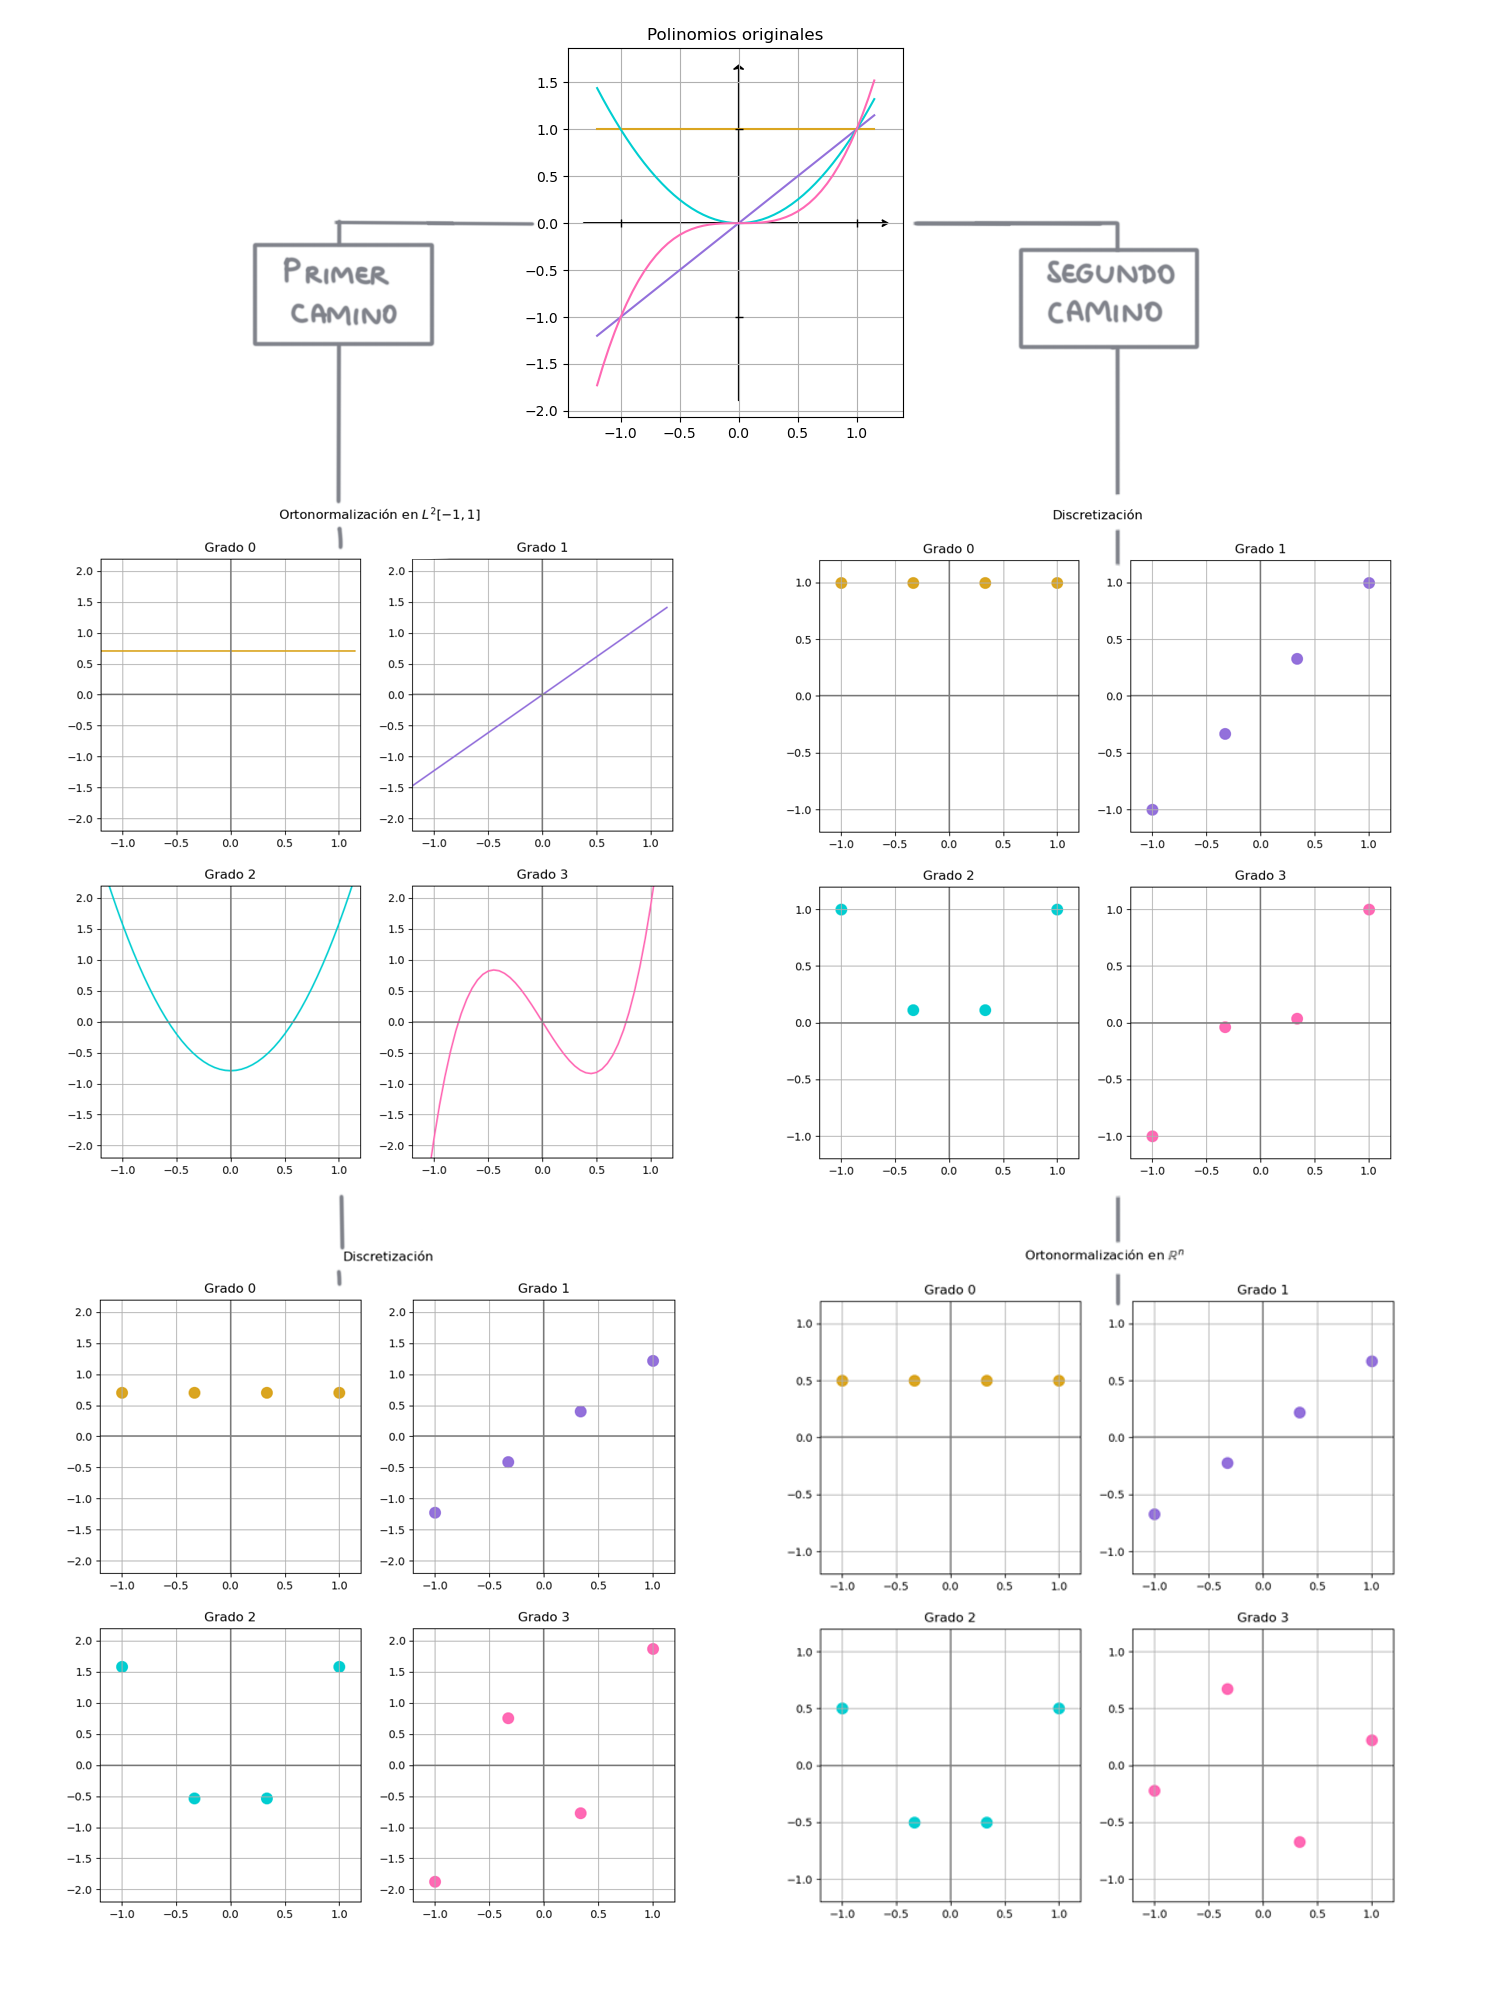
\includegraphics[scale=1.3]{discr_ortog} 
		\caption{Como se aprecia, las operaciones de
		ortogonalización y discretización no son conmutativas.}
 	\end{measuredfigure}
 \end{figure} %Sí compila
\section{Construcción canónica de la base de Legendre discreta}

Comenzamos planteando algunas definiciones.

\subsection{Discretización puntual, polinomios discretos y espacios asociados}
\label{discretizacion puntual, polinomios discretos y espacios asociados}

\begin{marginfigure}
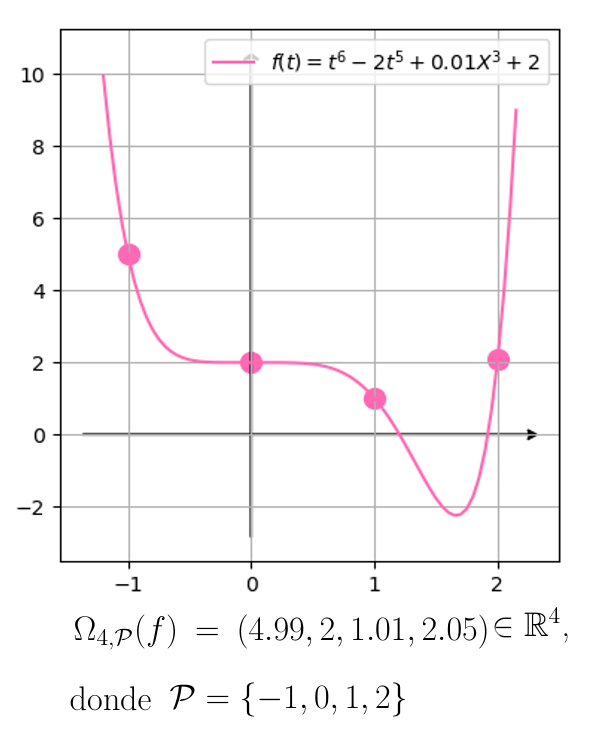
\includegraphics[scale=0.9]{1En_1} 
		\caption{Ejemplo concreto con $n=4$.}
\end{marginfigure}


\begin{defi}
\label{def: operador de discretizacion puntual}
(\textbf{Operador de discretización} $\Omega_{n,\cali{P}}$)
Sea $\cali{P}$ una malla uniforme 
de $n$ puntos
\[
\cali{P}:=\{ t_{j}:=t_{0}+hj : \hspace{0.1cm} 0 \leq j \leq n-1 \},
\]
donde $h \in \IR^{+}$ es una constante fija
(que llamamos el \textbf{paso} de la malla).
Nuestra primera forma de discretizar
a una función $f$ cuyo dominio contenga a los puntos
de la malla $\cali{P}$
consistirá en evaluarla en cada uno de los
puntos de la malla:

\begin{center}
$\Omega_{n,\cali{P}}(f) := (f(t_{j}))_{j=0}^{n-1}.$
\end{center}
\end{defi}


\noindent $\Omega_{n,\cali{P}}$
puede pensarse como una aplicación con dominio
$\cali{C}[t_{0}, t_{n-1}]$,
el espacio de funciones 
continuas en $[t_{0}, t_{n-1}]$,
y con codominio $\IR^{n}$, pero conviene 
identificar al resultado 
de la acción de $\Omega_{n,\cali{P}}$ sobre una
función $f$ con la restricción $f_{| \cali{P}}$
de 
$f$ al conjunto discreto $\cali{P}$,
es decir, con la función

\begin{center}
\aplica{f_{|\cali{P}}}
{\cali{P}}
{\IR }
{t_{j}}{f(t_{j}).}
\end{center}



\begin{defi} \label{def: polinomio discreto}
En el caso en el que $f$ sea elemento de $\IR[x]$, 
nos referiremos
al vector $\Omega_{n,\cali{P}}(f) \in \IR^{n}$
como un \textbf{polinomio discreto
de dimensión $n$ con dominio uniforme $\cali{P}$.} 
\end{defi} 

\sidenote{
En lo que sigue, siempre que se hable de un polinomio
discreto
se supondrá que la malla $\cali{P}$
a partir de la que se obtuvo es uniforme.}


Mostraremos en la subsección
\ref{definicion del concepto de grado para seniales finitas}
que, de hecho, \textbf{todo}
$x \in \IR^{n}$ es un polinomio discreto,
y daremos una definición del grado de este.
Ya podríamos dar algunos resultados en esta dirección,
pero preferimos esperar hasta tener las herramientas
para justificar detalles como la buena definición
de nuestra propuesta de grado.


Por la forma en que se definen la suma y la multiplicación
por escalares en los espacios vectoriales $\IR[x]$
y $\IR^{n}$, la siguiente observación es clara.

\begin{obs} \label{obs:linealidad de omega restringida a R[x]}
Sean $n \in \IN$ y $\cali{P}=\{t_{j}:
\hspace{0.2cm}0 \leq j \leq n-1 \}$ una malla uniforme
de $n$ puntos.
La función $\Omega_{n , \cali{P}}$ 
definida en 
\ref{def: operador de discretizacion puntual}
es una transformación lineal de 
$\cali{C}[t_{0}, t_{n-1}]$ a $\IR^{n}$.
\end{obs}
 


\begin{notacion} \label{notacion: Pn, fk, Wi, vk}
Sea $n \in \IN$ y $k$ un entero no negativo.
\footnote{Como se verá más adelante, 
nos interesarán sólo los enteros $k$
con $0 \leq k \leq n-1$.}.Denotaremos 
por $\IR_{k}[x]$ al subespacio de $\IR[x]$
que consta de los polinomios de grado a lo más $k$.
\noindent
Escribiremos como $f_{k}$ 
a las potencias básicas,
es decir, a los polinomios
\begin{equation}
\label{fk}
f_{k}(t):=t^{k}.
\end{equation}
Denotaremos por $\cali{P}_{n}$ a la siguiente
malla uniforme:
\begin{equation}
\label{malla Pn}
\cali{P}_{n}=\{ 0, 1, \ldots , n-1 \}.
\end{equation}
A la discretización puntual del
polinomio $f_{k}$ en la malla 
$\cali{P}_{n}$
la denotaremos por $v_{k}$;
\begin{equation}
\label{vectores vk}
v_{k}:= \Omega_{n, \cali{P}_{n}}(f_{k})
=(f_{k}(j))_{j=0}^{n-1}=(j^{k})_{j=0}^{n-1},
\end{equation}
y al subespacio de $\IR^{n}$ generado por los
primeros $i+1$ vectores $v_{k}$
(con $0 \leq i \leq n-1$ entero)
por por $W_{n,i}$;
\begin{equation}
\label{espacios Wi}
W_{n,i} := span\{ v_{k} : 0 \leq k \leq i \} \subseteq \IR^{n}.
\end{equation}
\end{notacion}


En la ecuación \eqref{espacios Wi} con la que se
define al espacio $W_{n,i}$,
siempre conviene pensar al primer subíndice $n$
como el \textbf{índice de dimensión}, pues corresponde
a la dimensión del espacio ambiente $\IR^{n}$,
y al subíndice $i$ como \textbf{índice de grado};
más adelante (c.f. tercer punto del teorema 
\ref{cor: propiedades importantes de espacios Wi}) 
se verá por qué este es un buen nombre.



\begin{obs} \label{obs:independencia lineal polinomios}
Sea $n \in \IN$. Si $i \in \overline{\IN}$, entonces
los $i+1$ polinomios
$f_{k}$ con $0 \leq k \leq i$ entero
constituyen una base para el espacio $\IR_{i}[x]$.
\end{obs}


\noindent
Como veremos a continuación, 
nuestras motivaciones geométricas
iniciales (el saber si la gráfica de una señal
de dimensión $n$ es afín o cuadrática) 
pueden reformularse en términos
de pertenencia a los espacios $W_{n,i}$.


\begin{prop} \label{obs: s en Wi sii es la discretizacion en malla Pn de un pol de grado a lo más i}
Sea $n \in \IN$.
Una señal $x=(x_{k})_{k=0}^{n-1}$ de dimensión $n$
es elemento del espacio $W_{n,i}$ 
definido en \eqref{espacios Wi}
si y sólo si 
$x$ es la discretización en $\cali{P}_{n}$
de un polinomio de grado a lo más $i$.
\end{prop}
\noindent
\textbf{Demostración.}
En efecto, según la definición del espacio
$W_{n,i}$ y la linealidad del operador
de discretización 
$\Omega$ establecida en 
la observación
\ref{obs:linealidad de omega restringida a R[x]}, 
tenemos que $x \in \IR^{n}$ es elemento de 
$W_{n,i}$ si y sólo si existen números reales
$a_{k}$ con $0 \leq k \leq i$ tales que
\begin{align*}
x=  \suma{k=0}{i}{a_{k}v_{k}} 
=  \suma{k=0}{i}{a_{k}\Omega_{n, \cali{P}_{n}}(f_{k})}
=  \Omega_{n, \cali{P}_{n}} \left( 
\suma{k=0}{i}{a_{k}f_{k}} \right)
=  \Omega_{n, \cali{P}_{n}} (g),
\end{align*}
con $g := \suma{k=0}{i}{a_{k}f_{k}} \in \IR_{i}[x]$
(c.f. observación 
\ref{obs:independencia lineal polinomios}).
\null\nobreak\hfill\ensuremath{\square} %final dem


\begin{cor} \label{cor: condiciones necesarias y suficientes para que x sea afín en términos de pertenencia a espacios Wi}
Sean $n \in \IN$ y $x \in \IR^{n}$ una señal de dimensión
$n$ cualquiera.
\begin{itemize}
\item La señal $x$ es constate si y sólo si $x \in W_{n,0}$,

\item es afín si y sólo si $x \in W_{n,1}$, y 

\item es cuadrática si y sólo si $x \in W_{n,2}$
y $x \not\in W_{n,1}$. \TODO{el último punto es claro? Tal vez lo sea
si este corolario va después.}
\end{itemize}
\end{cor}
\noindent
La importancia del corolario
\ref{cor: condiciones necesarias y suficientes para que x sea afín en términos de pertenencia a espacios Wi}
es que en él se explica cómo
\textbf{cuestiones de morfología de la señal $x$
se reducen a cuestiones de pertenencia a los espacios $W_{n,i}$}.
Parece pues que los espacios $W_{n,i}$ son un buen lugar
en el que buscar una base ortonormal con las propiedades
descritas en la lista 
de objetivos \ref{lista de objetivos}.

\noindent Demostremos ahora que,
en la proposición
\ref{obs: s en Wi sii es la discretizacion en malla Pn de un pol de grado a lo más i},
poco importa
la malla sobre la que se discretice, siempre y
cuando esta sea uniforme.


\begin{prop} \label{Obs1}
Si $\cali{P}$ es una malla
uniforme cualquiera de $n$ puntos, digamos
\[
\cali{P}= \{ t_{j}:= t_{0}+h :\hspace{0.1cm} 0 \leq l \leq n-1 \},
\]
con $h$ una constante positiva, 
y $f$ es un polinomio de grado $i$
(con $0 \leq i \leq n-1$),
entonces el vector $\Omega_{n, \cali{P}}(f)$ de $\IR^{n}$ 
es elemento del espacio $W_{n,i}$ definido en 
\eqref{espacios Wi}.
\end{prop}
\noindent
\textbf{Demostración.}
Según la observación \ref{obs:independencia lineal polinomios},
existen 
(únicos) números reales $c_{k}$, con $0 \leq k \leq i$
tales que 
$f= \suma{k=0}{i}{c_{k}f_{k}}$.
Sean los intervalos
\[
I_{n}=[0,n-1], \hspace{0.2cm} I=[x_{0}, x_{n-1}].
\]
Sea $\phi:I_{n} \longrightarrow I$ la función cuya gráfica
es el segmento de recta con puntos extremos 
\[
(0, t_{0}) \hspace{0.2cm} \text{y} \hspace{0.2cm}
(n-1, t_{n-1});
\]
la ecuación de tal $\phi$ es
\[
\phi(t)=ht+t_{0};
\] observe que $\phi$
es una recta con pendiente $h$ positiva.
Como tanto
$\cali{P}_{n}$ como $\cali{P}$
son mallas uniformes, 
\[
\forall \hspace{0.2cm} 0 \leq j \leq n-1: \hspace{0.2cm} \phi(j)=t_{j}.
\] 
(para convencerse de que esto ocurre
basta aplicar un argumento de semejanza de triángulos).
\noindent Así, la $(j+1)$-ésima entrada del
vector $\Omega_{n, \cali{P}}(f)=(f(t_{j}))_{j=0}^{n-1}$ es
\[
f(t_{j})= f (\phi (j))=
f(hj+t_{0})=
\suma{k=0}{i}{c_{k}f_{k}(hj+t_{0})}
= \suma{k=0}{i}{c_{k}(hj+t_{0})^{k}}.
\]
Reconocemos al lado derecho de la igualdad como un polinomio
de grado a lo más $i$, a saber,
\[
h(x):= \suma{k=0}{i}{c_{k}(hx+t_{0})^{k}}
\]
evaluado en el $(j+1)$-ésimo elemento 
de la malla uniforme $\cali{P}_{n}$
(o sea, en $j$). Según la observación
\ref{obs: s en Wi sii es la discretizacion en malla Pn de un pol de grado a lo más i}
de esto podemos concluir la pertenencia de 
$\Omega_{n, \cali{P}}(f)$ a $W_{n,i}$. \\

\begin{figure}[H]
	\sidecaption{
	Ejemplo haciendo $n=11$, $\cali{P}$ la malla
	uniforme de $11$ puntos con punto inicial $-2$
	y paso $h=0.5$.	    
	A la izquierda se dibuja la gráfica de 
	$f(t)=t^{3}-3t+1$
	y su discretización puntual en $\cali{P}$.
	A la derecha, la gráfica de $\phi(t)=0.5t-2$. A  
    una tal función lineal $\phi$ le llamaremos, en este contexto,
    \textbf{función de cambio de malla}.}
    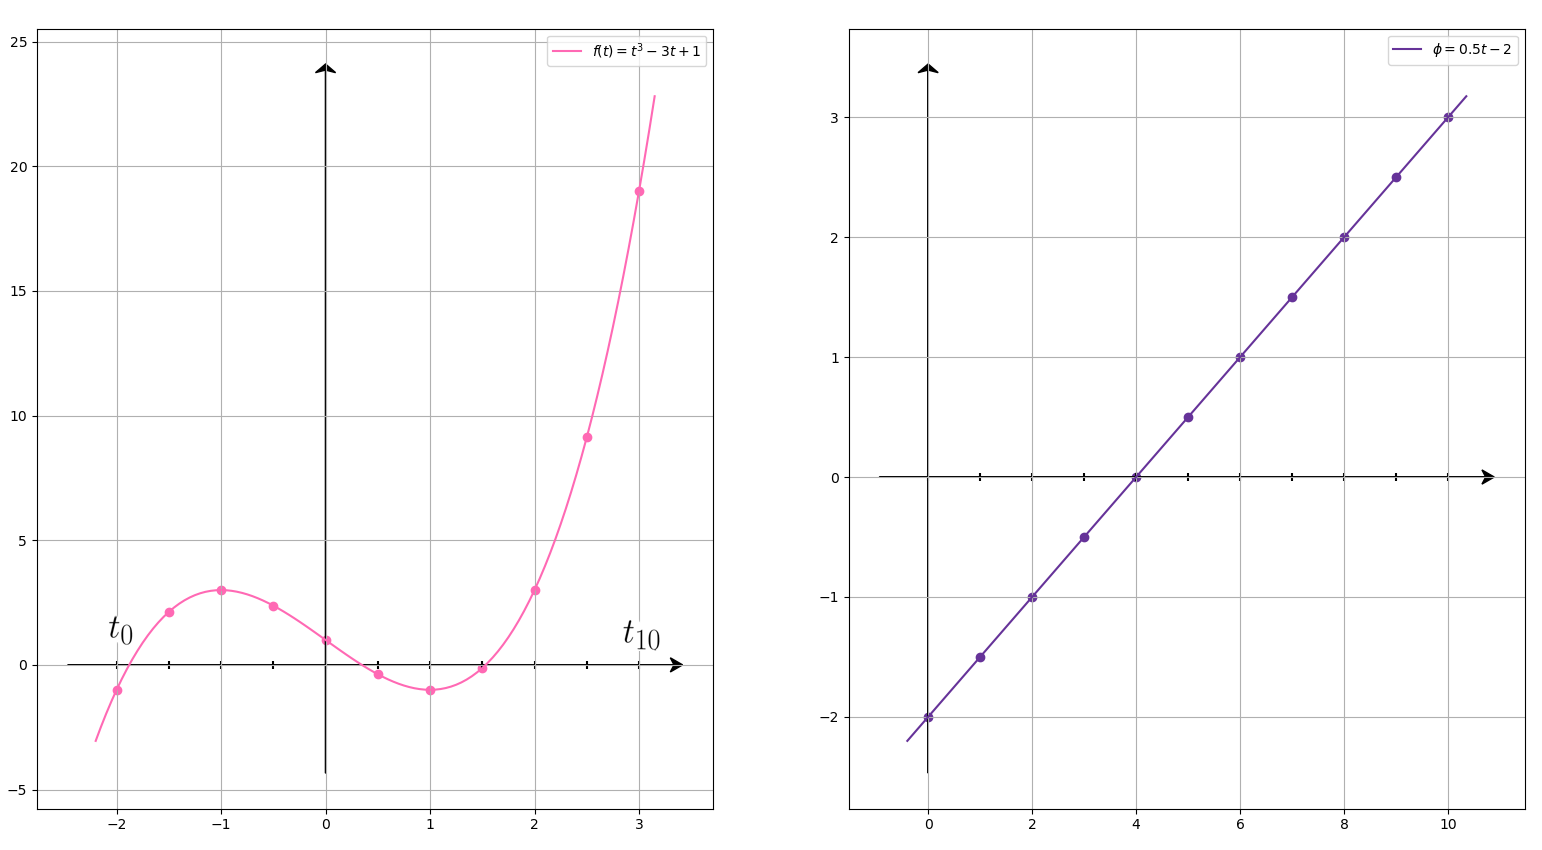
\includegraphics[scale=0.3]{mall} 
 \end{figure}
\QEDB
\vspace{0.2cm}

Concluimos así que
el subespacio de $\IR^{n}$
\begin{equation*}
\label{def de espacios Wk}
W_{n,i}= span\{ v_{k} : 0 \leq k \leq i \},
\end{equation*}
con $0 \leq i \leq n-1$ entero,
\textbf{es} el espacio de
los polinomios discretos
de dimensión $n$ con dominio uniforme 
\sidenote{
Una contención se 
prueba en la proposición 
\ref{obs: s en Wi sii es la discretizacion en malla Pn de un pol de grado a lo más i}
y la otra en la proposición \ref{Obs1}.
}
y
de grado a lo más $i$.



Como mostramos en el siguiente teorema, los vectores
$v_{k}$, con $0 \leq k \leq i$, más que un conjunto generador
del espacio $W_{n,i}$, conforman una base de este.


\begin{prop} \label{Teorema1}
Sea $n \in \IN$.
Si $0 \leq i \leq n-1$ es un entero y
\[
\{ p_{k}=p_{k}(t): \hspace{0.2cm} 0 \leq k \leq i \}
\]
es una colección de polinomios linealmente independientes, con
\[
\partial (p_{k})=k, \hspace{0.4cm} 0 \leq k \leq i
\]
y 
\[
\cali{P}= \{ t_{j}= t_{0}+hj :\hspace{0.1cm} 0 \leq j \leq n-1 \}
\]
es una malla uniforme cualquiera
de $n$ puntos, entonces los $i+1$ vectores
de $\IR^{n}$
\begin{equation}
\label{eq1: 30Oct}
w_{k} := \Omega_{n, \cali{P}}(p_{k}), \hspace{0.4cm} 0 \leq k \leq i
\end{equation}
son linealmente independientes.
\end{prop}
\noindent
\textbf{Demostración.}
Mostremos primero que $\{ w_{k}: \hspace{0.1cm} 0 \leq k \leq i \}$
es un subconjunto linealmente independiente de $\IR^{n}$.
Sean $b_{k}$ con $0 \leq k \leq i$ escalares
para los que se tenga la siguiente igualdad en $\IR^{n}$:

\begin{equation} \label{eq1: 3Agosto}
\suma{k=0}{i}{b_{k}w_{k}}=0.
\end{equation}

\noindent 
Según la linealidad establecida en la observación
\ref{obs:linealidad de omega restringida a R[x]}
y la definición \ref{eq1: 30Oct} de los vectores $w_{k}$,
si $p=p(t)$ es el polinomio
definido como
\begin{equation}
\label{eq2: 30Oct}
p:=\suma{k=0}{i}{b_{k}p_{k}},
\end{equation}
la ecuación \eqref{eq1: 3Agosto} puede reescribirse como

\begin{equation} \label{eq2: 3Agosto}
\Omega_{n , \cali{P}} (p) = 0.
\end{equation}

Ahora bien, 
la ecuación \eqref{eq2: 3Agosto}
expone a los $n$ puntos
de la malla $\cali{P}$ como raíces de $p$;  puesto que
el grado de $p$ es menor a $n$
(pues $p$ se ha definido en \eqref{eq2: 30Oct} como
combinación lineal de polinomios de grado menor
a $n$), 
concluimos, según la proposición \ref{prop: cita TFA},
que $p$ es el polinomio cero, 
y de esto, por la
independencia lineal de los polinomios $p_{i}$
en el espacio $\IR[x]$, la
igualdad a cero de los escalares $b_{k}$. 
\QEDB
\vspace{0.2cm}

\begin{prop}
Sea $n \in \IN$. Para todo entero $0 \leq i \leq n-1$, 
$\{v_{k}: \hspace{0.1cm} 0\leq k \leq i \}$ es una base
del espacio $W_{n,i}$
definido en \eqref{espacios Wi}.
\end{prop}
\noindent
\textbf{Demostración.}
Puesto que los polinomios $f_{k}$, con $0 \leq k \leq i$
satisfacen las hipótesis de la proposición \ref{Teorema1},
según este resultado
tenemos que los vectores $v_{k}= \Omega_{n, \cali{P}_{n}}(f_{k})$ 
con $0 \leq k \leq i$
son linealmente independientes; como estos, 
por definición,
generan al espacio $W_{n,i}$, concluimos que 
estos conforman una base de $W_{n,i}$.
\QEDB
\vspace{0.2cm}

Las propiedades más importantes de los
espacios $W_{n,i}$ (y que se desprenden
de los argumentos anteriores) se 
resumen en el siguiente teorema. 
Sólo del notar que las dimensiones de 
$\IR^{n}$ y su subespacio $W_{n, n-1}$
coinciden se deduce el cuarto punto.

\TODO{Por aquí di que a $W_{n,0}$ le llamarás
el espacio de $n-$dimensionales ctes etc... y en una
sidenote que, a pesar de que en $W_{n,2}$ puede haber señales
que no son cuadráticas (sino ctes y afines) usas ese nombre
para dar a entener euq en $W_{n,2}$ hay, a lo más, de grado 2.
Cuidado; aún no hablas del grado de una señal. Entonces, mejor
pon esto justo después.}

\begin{teo}
\label{cor: propiedades importantes de espacios Wi}
Sea $n \in \IN$. Sean, para cada $0 \leq i \leq n-1$,
los espacios $W_{n,i}$ como
se definieron en \eqref{espacios Wi}.
\begin{itemize}
\item Para toda $i$, $W_{n,i}$ es un subespacio
de $\IR^{n}$ de dimensión $i+1$. De hecho, 
$\{v_{k}: \hspace{0.1cm} 0\leq k \leq i \}$, con
$v_{k}$ definido como en \eqref{vectores vk},
es base de $W_{n,i}$.

\item La familia $(W_{n,i})_{i=0}^{n-1}$ de subespacios
	de $\IR^{n}$ está estríctamente anidada, es decir
	\begin{equation}
	\label{espacios Wi estan anidados}
	\forall \hspace{0.1cm}
	0 \leq i \leq n-2: \hspace{0.2cm}
	W_{n,i} \subsetneq W_{n,i+1}.
	\end{equation}

\item El espacio $W_{n,i}$ consta \textbf{exactamente}
de los polinomios discretos de dimensión $n$ con dominio uniforme
de grado a lo más $i$.

\item $\IR^{n}= W_{n,n-1}$.
\end{itemize}
\end{teo}

\begin{figure}[H]
\centering\captionsetup{format = hang}
	\begin{measuredfigure}
		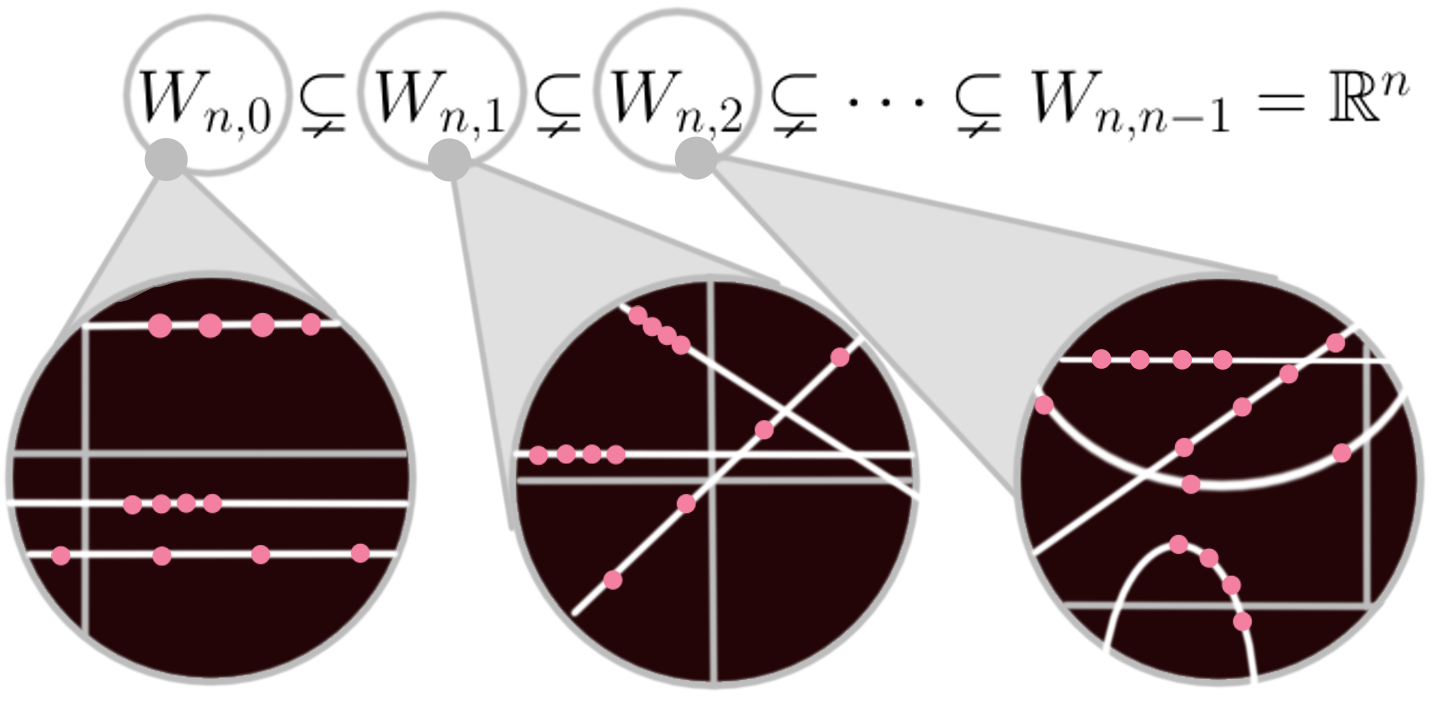
\includegraphics[scale=1]{nuevas_lupas} 
		\caption{
	En la figura	
	se dibujan las gráficas de algunos de los elementos
	de los tres primeros espacios de polinomios discretos
	$W_{n,0}$, $W_{n,1}$ y $W_{n,2}$
	(en la figura se ha fijado $n=4$).
    Observe que estas son
	las formas de recta y parábola de
	nuestro interés. 
	Queremos hacer énfasis en que, tomando
	\textbf{cualquier} malla uniforme y \textbf{cualquier} 
	polinomio $f$
	de grado $0 \leq i \leq n-1$, estamos seguros de que
	la discretización $\Omega_{n, \cali{P}}(f)$ es elemento
	del subespacio $W_{n,i}$ de $\IR^{n}$; reciprocamente, el 
	saber que un $x \in \IR^{n}$ sea elemento 
	de algún espacio $W_{n,i}$ (hecho
	que, en vistas de que la familia $(W_{n,i})_{i=0}^{n-1}$
	``cubre de manera ascendente a todo el espacio $\IR^{n}$''
	(c.f. puntos dos y cuatro del teorema 
	\ref{cor: propiedades importantes de espacios Wi}), seguro 
	ocurrirá), nos permite hacer inferencias sobre la forma 
	de la gráfica de $x$.}
 	\end{measuredfigure}
 \end{figure}





\subsection{Una definición del concepto de grado para señales finitas}
\label{definicion del concepto de grado para seniales finitas}

Revise nuevamente el último punto del teorema
\ref{cor: propiedades importantes de espacios Wi}; según este,
como se anticipó en la subsección 
\ref{discretizacion puntual, polinomios discretos y espacios asociados},
toda señal finita $x \in \IR^{n}$
es elemento de $W_{n,n-1}$,
es decir, es un polinomio discreto
de dimensión $n$ y grado menor a $n$.

Podemos dar una demostración
alternativa,
directa y sencilla de este hecho.

\begin{prop}
\label{prop: el operador de discretizacion puntual es un isomorfismo (...)}
Sean $n \in \IN$, $\cali{P}$ una malla uniforme de $n$
puntos. 
La restricción del operador $\Omega_{n, \cali{P}}$
al espacio $\IR_{n-1}[x]$ de polinomios de grado a lo más
$n-1$, es decir, la función 
\begin{equation}
\label{eq0: 28Nov}
\Omega_{n, \cali{P}}:
\IR_{n-1}[x] \longrightarrow \IR^{n}
\end{equation}
es un isomorfismo de $\IR-$espacios vectoriales.
En particular, para todo vector $x \in \IR^{n}$
existe un único polinomio $f$ de grado menor a n
tal que $x = \Omega_{n, \cali{P}}(f)$.
\end{prop}
\noindent
\textbf{Demostración.}
Puesto que tanto $\IR_{n-1}[x]$
como $\IR^{n}$ son $\IR$-espacios vectoriales
de dimensión $n$, para ver que la función 
\eqref{eq0: 28Nov} (que, según la observación 
\ref{obs:linealidad de omega restringida a R[x]}, es lineal)
es un isomorfismo, basta
demostrar que es inyectiva 
(c.f. teorema 2.5 \TODO{Friedberg}).
Esto último es una consecuencia directa del 
teorema fundamental del álgebra,
pues, 
$f \in \IR_{n-1}(x)$
es elemento del kernel
de \eqref{eq0: 28Nov} si y sólo si 
$\Omega_{n, \cali{P}}(f)=0$, o, equivalentemente,
si y sólo si 
cada uno de los $n$ puntos que componen la
malla $\cali{P}$ es una raíz de $f$. Puesto que
$f$ es un polinomio de grado a lo más $n-1$
(y, por lo tanto, de no ser el polinomio cero tiene
a lo más $n-1$ raíces reales),
esto último ocurre si y sólo si $f$ es el polinomio cero.
Con esto comprobamos que el kernel de la aplicación
\label{eq1: 25Nov} es trivial, luego, la inyectividad
de esta.
\QEDB
\vspace{0.2cm}

La proposición
\ref{prop: el operador de discretizacion puntual es un isomorfismo (...)}
parece sugerir 
una forma en la que podríamos 
definir el grado de 
un vector $x \in \IR^{n}$ (``dado $x \in \IR^{n}$, definimos
el grado de este como el grado del único polinomio $f \in \IR_{n-1}[x]$
tal que $\Omega_{n, \cali{P}}(f)=x$''); no hay
que apresurarse, pues en la formulación de
la proposición
\ref{prop: el operador de discretizacion puntual es un isomorfismo (...)}
se tuvo que fijar de antemano una malla uniforme.
\textit{A priori}, no podríamos descartar 
la existencia de mallas uniformes
$\cali{P}, \tilde{\cali{P}}$ 
de $n$ puntos
y de polinomios
$f, \tilde{f}$ de grados menores a $n$ (pero no 
iguales entre sí), tales que
$\Omega_{n, \cali{P}}(f) = x = \Omega_{n, \tilde{\cali{P}}}(\tilde{f})$.
Comprobamos que esto no ocurre
en el siguiente resultado.

\begin{figure}[H]
	\sidecaption{Lo que sí es seguro es que la unicidad establecida en la proposición \ref{prop: el operador de discretizacion puntual es un isomorfismo (...)} no es válida si se quita la restricción en los grados de los polinomios a discretizar.
	\label{fig: restriccion en grado pol}
	}
	\centering
	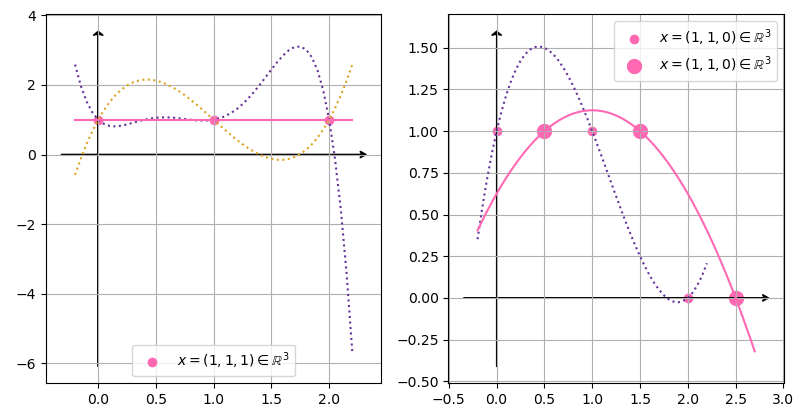
\includegraphics[scale=0.52]{25Nov_1} 
\end{figure}	


\begin{prop}
\label{prop: igualdad de grado (menor a n) si dos polinomios al discretizarse dan x}
Sean $n \in \IN$, $x \in \IR^{n}$.
Si $\cali{P}, \tilde{\cali{P}}$ son mallas uniformes
de $n$ puntos y $\tilde{f}, f \in \IR_{n-1}[x]$
son tales que
\begin{equation}
\label{eq2: 25Nov}
\Omega_{n, \tilde{\cali{P}}}(\tilde{f})= x = 
\Omega_{n, \cali{P}}(f),
\end{equation}
entonces $\partial(\tilde{f})=\partial(f)$.
\end{prop}
\noindent
\textbf{Demostración.}
Digamos que 
\[
\cali{P}=\{t_{j}:=t_{0}+hj: \hspace{0.2cm} 0 \leq j \leq n-1 \},
\hspace{0.2cm}
\cali{\tilde{P}}=\{
\tilde{t_{j}}:=\tilde{t_{0}}+ \tilde{h}j: \hspace{0.2cm} 0 \leq j \leq n-1 \}.
\]
Sea 
\[
\phi(t)= \frac{h}{\tilde{h}}t+ \left( t_{0}-  \frac{h}{\tilde{h}}
\tilde{t_{0}}  \right)
\]
la función de cambio de malla
(de $\tilde{\cali{P}}$ a $\cali{P}$); esta función es 
tal que
\[
\forall \hspace{0.1cm} 0 \leq j \leq n-1, 
\hspace{0.5cm} \phi(\tilde{t_{j}})= 
t_{j};
\]
podemos reescribir entonces la hipótesis \eqref{eq2: 25Nov}
como 
\begin{align*}
(\tilde{f}(\tilde{t_{0}}), \ldots , \tilde{f}(\tilde{t_{n-1}}))
= & x \\
=& (f(t_{0}), \ldots , f(t_{n-1})) \\
=& ((f \circ \phi) (\tilde{t_{0}}), \ldots , 
(f \circ \phi) (\tilde{t_{n-1}})),
\end{align*}
o sea, como $\Omega_{n, \tilde{\cali{P}}}(\tilde{f})=
\Omega_{n, \tilde{\cali{P}}}(f \circ \phi)$; por linealidad
del operador $\Omega_{n, \tilde{\cali{P}}}$
(c.f. observación 
\ref{obs:linealidad de omega restringida a R[x]})
tenemos entonces que
$\Omega_{n, \tilde{\cali{P}}}(\tilde{f}-f \circ \phi)=0$,
o sea, que 
$\tilde{f}-f \circ \phi$ es un polinomio de
grado menor a $n$ con al menos $n$ raíces 
(a saber, los $n$ elementos de $\tilde{\cali{P}}$), luego, 
según la proposición \ref{prop: cita TFA},
$\tilde{f}-f \circ \phi$
es el polinomio cero, por lo tanto, 
\begin{equation*}
\label{eq3: 25Nov}
\tilde{f}=f \circ \phi.
\end{equation*}

Puesto que el componer a $f$ con el polinomio lineal
$\phi$ no altera su grado (i.e. $f$ y $f \circ \phi$
son polinomios del mismo grado), concluimos que
\[
\partial(\tilde{f})= \partial(f \circ \phi)=
\partial(f).
\]
\QEDB
\vspace{0.2cm}

Con todo esto demostrado, podemos definir
el grado de una señal finita como sigue.

\begin{defi}
\label{def: del grado de una senial finita}
Sean $n \in \IN$, $x \in \IR^{n}$.
Si $f \in \IR_{n-1}[x]$
es un polinomio de grado menor a $n$
y $\cali{P}$ es una malla uniforme
de $n$ puntos tales que
$x= \Omega_{n, \cali{P}}(f)$, entonces
el \textbf{grado de $x$} es 
\[
\partial(x):= \partial(f).
\]
\end{defi}


Es fácil determinar el grado de una señal 
de dimensión $n$
en términos de pertencia a los espacios $W_{n,i}$;
mostramos a continuación que
el grado $i$ de un polinomio discreto es el índice
del menor subespacio $W_{n,i}$ en el que está contenido.

\begin{prop}
Sean $n \in \IN$ y $x \in \IR^{n}$ una señal de dimensión $n$.
\begin{itemize}
\item $x$ tiene grado cero si y sólo si $x \in W_{n,0}$.
\item Para toda $1 \leq i \leq n-1$,
$x$ tiene
grado $i$ si y sólo si 
$x \in W_{n,i}$ pero $x \not\in W_{n,i-1}$.
\end{itemize}
\end{prop}
\noindent
\textbf{Demostración.}
La veracidad del primer punto de la demostración
es obvia (pues $W_{n,0}$ consta exactamente de las discretizaciones
puntuales de polinomios constantes, c.f. 
teorema \ref{cor: propiedades importantes de espacios Wi}).
Demostremos pues el segundo punto.

\begin{itemize}
\item [$\Rightarrow$)]

Supongamos que $\partial(x)=i$ con $1 \leq i \leq n-1$;
por definición, esto significa que existen
$\cali{P}$ una malla uniforme de $n$ puntos y $f$ un 
polinomio 
tales que 
\begin{equation}
\label{eq5: 25Nov}
\partial(f)=i \hspace{0.2cm} \text{y} \hspace{0.2cm}
x=\Omega_{n,\cali{P}}(f).
\end{equation}
Según la proposición 
\ref{Obs1},
esto implica la pertenencia de $x$ a $W_{n,i}$.
Además, $x$ no puede ser elemento de $W_{n,i-1}$,
pues esto,
según el tercer punto del corolario
\ref{cor: propiedades importantes de espacios Wi},
implicaría la existencia de una
malla uniforme $\tilde{\cali{P}}$ de $n$
puntos y un polinomio $g$ tales que
\begin{equation}
\label{eq6: 25Nov}
\partial(g)\leq i-1 \hspace{0.2cm} \text{y} \hspace{0.2cm}
x=\Omega_{n,\tilde{\cali{P}}}(g);
\end{equation}
según la proposición
\ref{prop: igualdad de grado (menor a n) si dos polinomios al discretizarse dan x}, \eqref{eq5: 25Nov}
y \eqref{eq6: 25Nov} no pueden ser ambas verdaderas.

\item[$\Leftarrow$)] Sea
$1 \leq i \leq n-1$ tal que $x \in W_{n,i}$
pero $x \not\in W_{n,i-1}$.
Según el corolario
\ref{cor: propiedades importantes de espacios Wi}, existen
$\cali{P}$ malla uniforme de $n$ puntos y
$f$ polinomio de grado a lo más $i$ tales que
$x= \Omega_{n, \cali{P}}(f)$; según este mismo
corolario, el que el grado de $f$ fuese menor a $i$
implicaría que $x$ también fuese elemento
del espacio $W_{n,i-1}$. Como esto no ocurre, concluimos
que $x= \Omega_{n, \cali{P}}(f)$
con $\partial(f)=i$, luego, según la definición
\ref{def: del grado de una senial finita}, 
$x$ tiene grado $i$.
\end{itemize}
\QEDB
\vspace{0.2cm}




\subsection{Construcción de la base de Legendre discreta via ortogonalización de bases de espacios de polinomios discretos}

\noindent Ahora, con el proceso de Gram-Schmidt \ref{Prop:Gram-Schmidt2}
vamos a normalizar
a la base $\{v_{k}: \hspace{0.1cm} 0 \leq k \leq n-1 \}$ de
$W_{n,n-1}$, o sea, de $\IR^{n}$ (c.f. 
cuarto punto del teorema
\ref{cor: propiedades importantes de espacios Wi}). 
Por la naturaleza del proceso, durante este se
obtienen bases ortonormales para cada uno de los espacios 
$W_{n,i}$. \TODO{detalla mejor esto.}

%\begin{figure}[H]
%   \centering
%   \incfig{28JunioInks}
%    \caption{ 
%    \TODO{Cambiar notación espacios W}
%    Como muestra el diagrama, 
%	lo que se hace es proyectar el vector $v_{k}$, con
%	$1 \leq k \leq n-1$, al espacio
%	$W_{n,k-1}$ para así 
%	formar al vector $\bar{\xi}_{k}$ y después
%	normalizarlo.}
%\end{figure}


\begin{defi} 
\label{def: base de Legendre discreta}
A la base ortonormal de $\IR^{n}$
\begin{equation}
\label{eq: base de Legendre discreta}
\cali{L}^{n}=\{ \cali{L}^{n,k}= (\cali{L}_{m}^{n,k})_{m=0}^{n-1} \in \IR^{n}: 
\hspace{0.1cm} 0 \leq k \leq n-1\}
\end{equation}
que resulta de ortonormalizar con G-S a la base
\[
\{v_{k} \in \IR^{n}: \hspace{0.1cm} 0 \leq k \leq n-1 \}
\]
de $\IR^{n}$ la llamaremos la
\textbf{base de Legendre discreta de dimensión $n$}.

Denominaremos a la señal $\cali{L}^{n,k}$ el 
\textbf{polinomio discreto de Legendre de dimensión
$n$ y grado $k$}.
\end{defi}

\begin{cor} \label{cor: BON de legendre para espacios Wk}
Sea $n \in \IN$. Para todo $0 \leq k \leq n-1$, los vectores
\[
\cali{L}^{n, l}, \hspace{0.2cm} 0 \leq l \leq k
\]
conforman una BON del espacio $W_{n,k}$.
\end{cor}

\begin{cor} \label{cor: Ln,k ortogonal a todo pol discreto de grado menor a k}
Sea $n \in \IN$. Si $k$ es un entero con $1 \leq k \leq n-1$,
entonces
\[
\forall \hspace{0.1cm} 0 \leq l \leq k-1:
\hspace{0.2cm}
\cali{L}^{n,k} \in W_{n,l}^{\perp},
\]
o sea, 
$\cali{L}^{n,k}$ es ortogonal a todo polinomio discreto
de grado menor a $k$.
\end{cor}
\noindent
\textbf{Demostración.}
En efecto, según la definición
\ref{def: base de Legendre discreta}, 
$\cali{L}^{n,k}$ es ortogonal a todos los vectores
$\cali{L}^{n, l}$ con $0 \leq l \leq k$,
luego, según el corolario
\ref{cor: BON de legendre para espacios Wk},
ortogonal a toda una base del espacio $W_{n,k}$,
por lo tanto, a todo elemento de este.
\QEDB
\vspace{0.2cm}



\begin{center}
{\Huge{
$\cali{L}^{\textcolor{ameMorado}{n}, 
\textcolor{ameDorado}{k}}=
\left(
\cali{L}^{\textcolor{ameMorado}{n}, 
\textcolor{ameDorado}{k}}_{\textcolor{ameRosa}{m}}
\right)_{m=0}^{m=n-1} \in \IR^{n}
$}}
\end{center}
\begin{itemize}
\item \textcolor{ameMorado}{n} $\in \IN$: dimensión del espacio ambiente
\item $0 \leq  \textcolor{ameDorado}{k} \leq n-1$ entero: parámetro de grado
\item $0 \leq \textcolor{ameRosa}{m} \leq n-1$ entero: parámetro de posición
\end{itemize}
\TODO{Hacer eso una imagen. Tratamos de usar consitentemente la notación
explicada en la figura a lo largo del texto.} %Sí compila
\input{propiedades_Legendre} %parece que hay un error.
\section{Ejemplos}
\label{sec: ejemplos}
Definidas ya las bases de Legendre discretas
para toda dimensión $n$ 
(c.f. definición  
\ref{def: base de Legendre discreta}) y estudiadas algunas de sus 
propiedades, planteemos algunos ejemplos
para constatar en dimensiones concretas algunos de los
resultados demostrados en subsecciones anteriores
y empezar a comprobar la utilidad de estas bases para el 
estudio morfológico de señales finitas.


%Inicio ejemplo 1--------------------------------------------
\begin{ejemplo}
A continuación, mostramos las gráficas de los
elementos de las bases $\cali{L}^{2}$ y $\cali{L}^{3}$.
Para dibujar las gráficas usamos los valores
calculados en la tabla
\ref{formulas explicitas para Ln con n de 2 hasta 6}.

\begin{figure}[H]
	\sidecaption{
	Gráficas de los elementos de $\cali{L}^{2}
	\subseteq \IR^{2}$
	\label{fig: graficas elementos L2}
	}
	\centering
	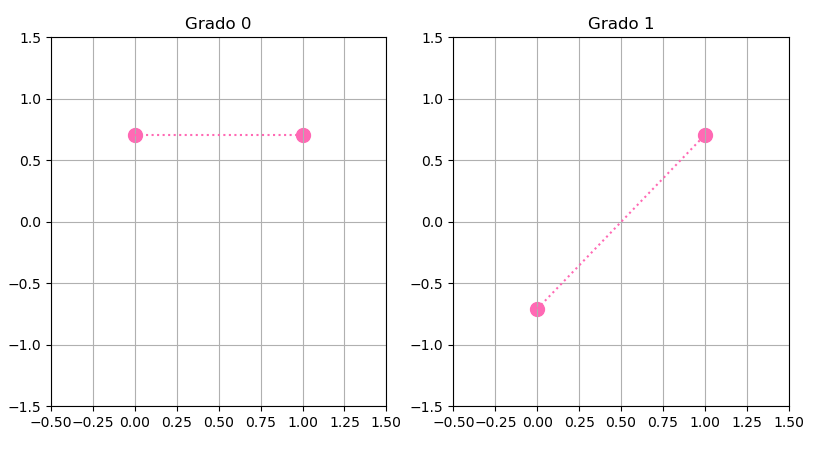
\includegraphics[scale=0.5]{graficasLegendre2} 
\end{figure}	


\begin{figure}[H]
	\sidecaption{
	Gráficas de los elementos de $\cali{L}^{3} 
	\subseteq \IR^{3}$
	\label{fig: graficas elementos L2}
	}
	\centering
	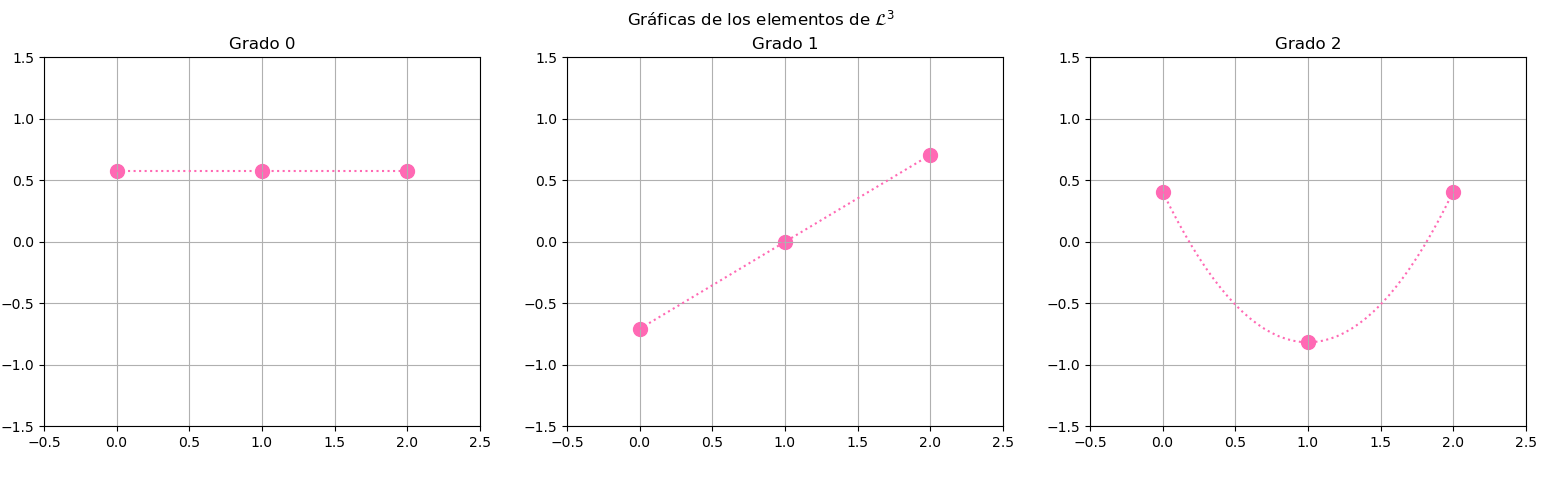
\includegraphics[scale=0.26]{graficasLegendre3} 
\end{figure}	




En el caso $n=2$, el único subespacio de polinomios
discretos no trivial es 
\begin{align*}
W_{2,0}= & span \left\{ 
\left(\frac{1}{\sqrt2}, \frac{1}{\sqrt2} \right) \right\} \\
= & \{ (x,x) \in \IR^{2}: \hspace{0.2cm} x \in \IR \},
\end{align*}

pues

\begin{equation}
\label{eq1: 1Dic}
W_{2,1}= \IR^{2}.
\end{equation}


En el caso $n=3$, calculamos que
\begin{align*}
W_{3,0}= & span \left\{
\left( \frac{1}{\sqrt3}, \frac{1}{\sqrt3},
\frac{1}{\sqrt3} \right) \right\}  \\
= & \{ (x,x,x) \in \IR^{3}: \hspace{0.2cm} x \in \IR \},
\end{align*}

\begin{align}
\label{eq2: 1Dic}
W_{3,1}= & span \left\{ \left( \frac{1}{\sqrt3}, \frac{1}{\sqrt3},
\frac{1}{\sqrt3} \right) ,
\left( -\frac{1}{\sqrt2}, 0,  \frac{1}{\sqrt2} \right) \right\}
\nonumber \\
= & \{ (x,y,2y-x) \in \IR^{3}: \hspace{0.2cm} x,y \in \IR \},
\end{align}
y
\[
W_{3,2}=\IR^{3}.
\]

\begin{figure}[H]
	\sidecaption{
	Gráficas de 
	$W_{2,0} \subseteq \IR^{2}$
	y de los subespacios
	$W_{3,0}$ y $W_{3,1}$ de $\IR^{3}$ que
	son, respectivamente, una recta y un plano;
	observe que
	$W_{3,0} \subseteq W_{3,1}$. 
	En ambas dimensiones se han 
	dibujado en {\color{ameMorado}{morado}} a los hiperplanos
	de polinomios discretos correspondientes, que en efecto
	dividen en dos regiones ajenas a los respectivos espacios 
	ambiente. La definición de hiperplano se da en
	\ref{section: hiperplanos}.
	\label{fig: graficas espacios W para dimensiones 2 y 3}
	}
	\centering
	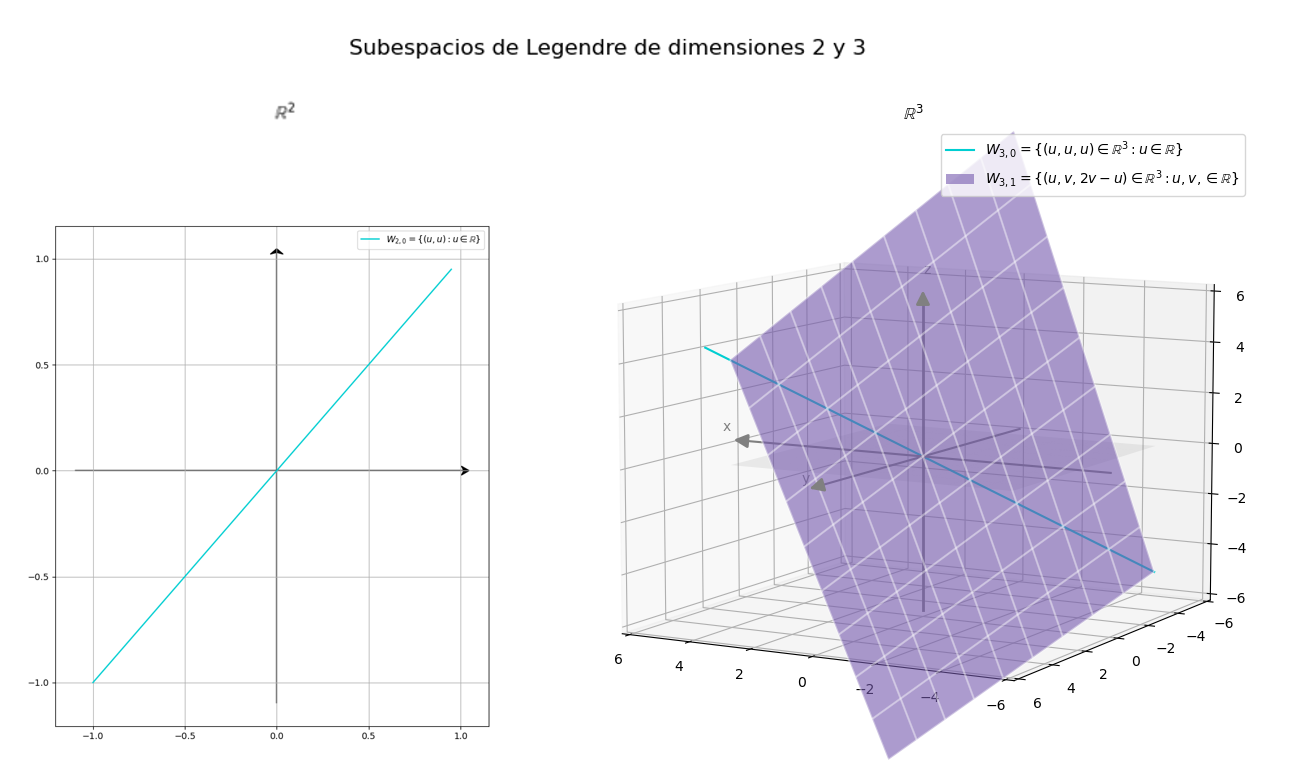
\includegraphics[scale= 1]{legendre2y3} 
\end{figure}	
	 
\final
\end{ejemplo}
%final ejemplo 1--------------------------------------------





%Inicio ejemplo 2--------------------------------------------

\begin{ejemplo}
Considere al siguiente conjunto de cinco
puntos del plano:
\begin{equation} \label{eq: conjunto cinco puntos}
\{ (0,-0.5), (1,2.4), (2, 1.6), (3,1.7), (4, 2.3) \}.
\end{equation}


Como tenemos cinco puntos, trabajamos
en el espacio $\IR^{5}$. 
La regresión lineal calculada a partir
del conjunto de datos
\eqref{eq: conjunto cinco puntos}
es la recta
con ecuación cartesiana

\begin{equation} \label{eq: recta minimos cuadrados}
y=0.49x+0.52.
\end{equation}

El vector cuyas entradas
son las cinco mediciones (dadas por las ordenadas
de los puntos del conjunto \eqref{eq: conjunto cinco puntos})
es
\begin{equation}
\label{eq0: 29Nov}
x=(-0.5, 2.4, 1.6, 1.7, 2.3).
\end{equation}


\begin{figure}[H]
	\sidecaption{
	Gráfica de la señal $x \in \IR^{5}$.
	\label{fig: grafica semal x ejemplo}
	}
	\centering
	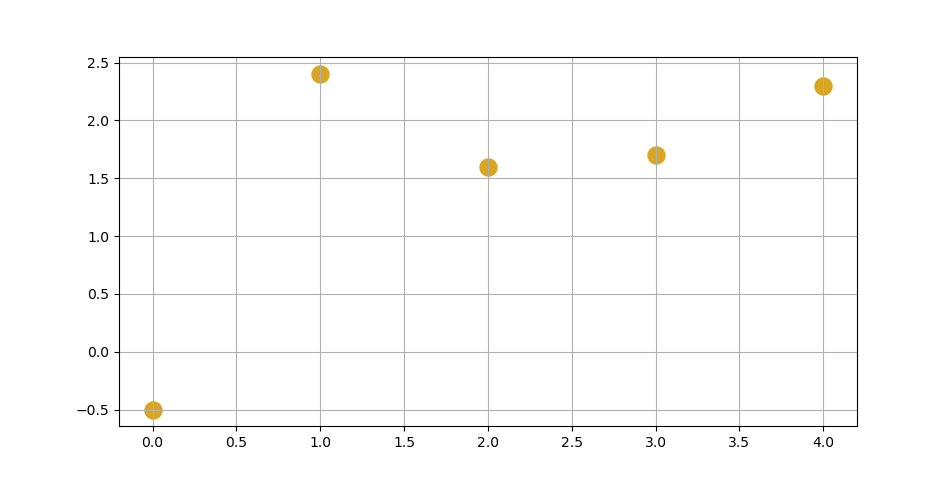
\includegraphics[scale=0.4]{graficaX_31Oct} 
\end{figure}	


Nos interesa
dar explícitamente a 
la señal $\Pi_{W_{5,1}}(x) \in W_{5,1} \leq \IR^{5}$.
En realidad, por ser $\cali{L}^{5}$ 
una base ortonormal de $\IR^{5}$ y por ser
$W_{5,1}$ el subespacio generado por los
dos primeros vectores de esta base, 
se sabe de inmediato que
\[
\Pi_{W_{5,1}}(x)=  \langle \Pi_{W_{5,1}}(x), \cali{L}^{5,0} \rangle \cali{L}^{5,0}
+ \langle \Pi_{W_{5,1}}(x), \cali{L}^{5,1} \rangle \cali{L}^{5,1};
\]
de todas formas, como ilustración, planteemos un sistema
de ecuaciones para llegar a una expresión para
$\Pi_{W_{5,1}}(x)$.
Usando las expresiones para los vectores
de $\cali{L}^{5}$
dadas en \ref{subsect:Formulas explicitas},
tenemos que
\[
W_{5,1}=span\{ (1,1,1,1,1,1), (-2, -1, 0, 1, 2) \},
\]

y 
\[
W_{5,1}^{\perp}=span\{ (2,-1,-2,-1,2), (-1,2,0,-2,1), (1,-4,6,-4,1)\}.
\]
Según el teorema de la proyección ortogonal \ref{Teo:proyOrt},
$\Pi_{W_{5,1}}(x)$ es el único elemento de $W_{5,1}$ para el 
que 

\[
x-\Pi_{W_{5,1}}(x) \in W_{5,1}^{\perp};
\]
esto se 
traduce en la existencia de 
únicos escalares $c_{1}$, $c_{2}$,
$a_{1}$, $a_{2}$ y $a_{3}$ tales que
\[
x-c_{1}(1,1,1,1,1)-c_{2}(-2, -1, 0, 1, 2)
\]
es igual a 

\[
a_{1}(2,-1,-2,-1,2)+a_{2}(-1,2,0,-2,1)
+ a_{3}(1,-4,6,-4,1),
\]
\noindent
o sea, tales que

\begin{equation*}
\begin{cases}
-0.5-(c_{1}-2c_{2})=2a_{1}-a_{2}+a_{3}, \\
2.4-(c_{1}-c_{2})=-a_{1}+2a_{2}-4a_{3}, \\
1.6-c_{1}=-2a_{1}+6a_{3},\\
1.7-(c_{1}+c_{2})=-a_{1}-2a_{2}-4a_{3}, \\
2.3-(c_{1}+2c_{2})=2a_{1}+a_{2}+a_{3}.
\end{cases}
\end{equation*}
Resolviendo este sistema
de ecuaciones, encontramos que
$c_{1}=1.5$ y $c_{2}=0.49$. Así,




\begin{align}
\label{eq5: 23Oct}
\Pi_{W_{5,1}}(x) =& c_{1} (1,1,1,1,1) + c_{2}(-2-1,0,1,2) \nonumber \\
= & (0.52, 1.01, 1.5, 1.99, 2.48 );
\end{align}
observe que \eqref{eq5: 23Oct} es, 
en efecto, la discretización de 
la recta \eqref{eq: recta minimos cuadrados}
en la malla uniforme $\cali{P}_{5}$.
De forma análoga se calcula la parte cuadrática de
la señal $s$.

\begin{figure}[H]
	\sidecaption{
	Gráficas de $x$, 
	$\Pi_{W_{5,0}}(x)$, $\Pi_{W_{5,1}}(x)$ y $\Pi_{W_{5,2}}(x)$.
	\label{fig: partes afin, lineal y cuadratica} 
	}
	\centering
	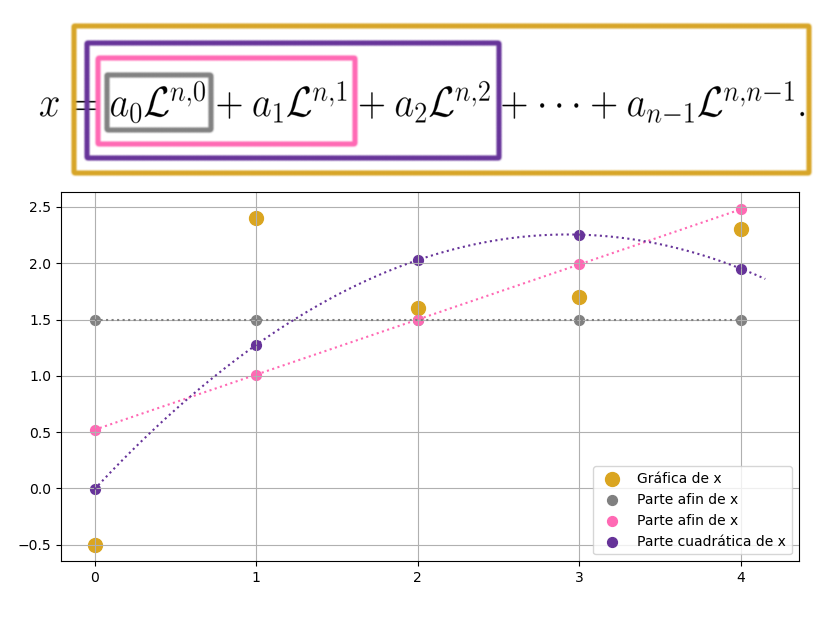
\includegraphics[scale=0.6]{parteAfinCuadr}
\end{figure}	
\final
\end{ejemplo}
%Final ejemplo 2--------------------------------------------


\TODO{Sería bueno notar que estas dando un
algoritmo de transformación de la raw data
via una proyección lineal (proceso mediante
en cual se destruye información). Nada de ML, 
esto es más bien symbolic AI (deep learning with
python, p.35)}



En el siguiente ejemplo 
damos dos propuestas naturales,
usando los espacios de polinomios discretos $W_{n,k}$,
para poder dar no sólo respuestas del tipo
``sí/no'' a preguntas sobre la morfología de una señal, sino,
de forma más general, del tipo ``qué tanto sí'' o
``qué tanto no''.



%Inicio ejemplo 3--------------------------------------------

\begin{ejemplo}
Hagamos $n=3$.  
Como se calculó en \eqref{eq2: 1Dic},
el subespacio $W_{3,1} \leq \IR^{3}$ de señales afines es el plano
de ecuación cartesiana

\[
W_{3,1}: \hspace{0.2cm} x-2y+z=0.
\]
Sea 
\begin{equation*}
\label{eq0: 9Feb}
x=a_{0}\cali{L}^{3,0}+a_{1}\cali{L}^{3,1}+a_{2}\cali{L}^{3,2}
\end{equation*}
un vector del espacio.
Como se argumentó ya, las proposiciones
\begin{center}
``$x \in \IR^{3}$ es afín'' \hspace{0.2cm} y \hspace{0.2cm} 
``$x \in W_{3,1}$''
\end{center} 
son equivalentes.
Observe que es ``poco probable'' que, al seleccionar al azar
un vector de $\IR^{3}$, este sea afín (pues el 
subconjunto $W_{3,1}$ de $\IR^{3}$,
un plano, tiene
medida de Lebesgue cero); sin embargo, provistos
de nociones como las de norma y ortogonalidad, es fácil dar 
propuestas legítimas de
\textbf{medidas} de ``qué tan afín'' es la señal $x$,
o, en términos matemáticos, de qué tanto se aleja
$x$ del espacio de señales afines de su correspondiente
espacio ambiente.

\begin{figure}[H]
	\sidecaption{
	Esquema de dos formas en las que uno puede intentar medir
	qué tan afín es una señal $x$.
	\label{fig: dos formas de medir distancia a plano}
	}
	\centering
	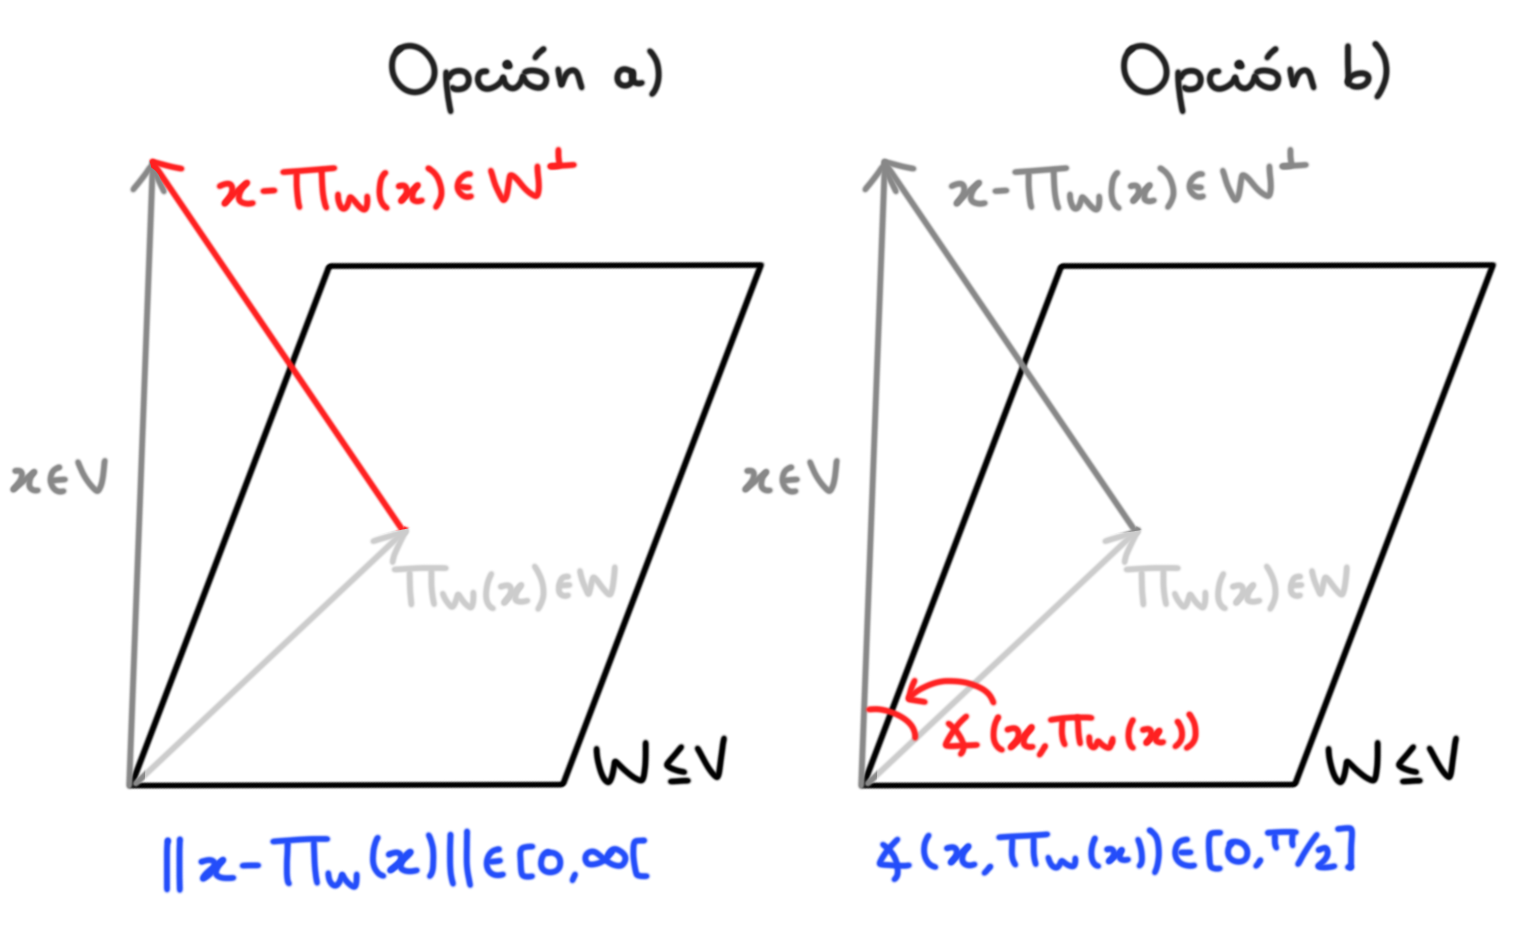
\includegraphics[scale= 1]{ 18Sept_1} 
\end{figure}	

\TODO{
Recuerda que debes de notar que la distancia al plano en realidad
no es la mejor forma de dar una medida de qué tan afín
es $x$.}

\begin{itemize}
\item[a)] Una forma obvia de proceder es calcular la norma
del vector 
\[
x - \Pi_{W_{3,1}}(x)= a_{2} \cali{L}^{3,2},
\]
es decir, tomar al número no negativo
\[
|a_{2}|
\]
como una medida de qué tanto se aleja $x$ del plano $W_{3,1}$
(o sea, de qué tanto se aleja $x$ de ser afín.)

\item[b)] Otro acercamiento podría ser preguntarse por
el ángulo $\alpha \in [0, \frac{\pi}{2}]$ 
que forma el vector $x$ con el espacio 
$W_{3,1}$. Los casos extremos $\alpha=0$ y $\alpha= \frac{\pi}{2}$
corresponden, respectivamente, a que $x$ sea afín y
a que $x$ sea múltiplo escalar de $\cali{L}^{3,2}$, luego,
a que sea ortogonal a cualquier señal afín de dimensión 3.

Como las dimensiones de $\IR^{3}$ y $W_{3,1}$ 
difieren por uno,
este útimo es un hiperplano
\sidenote{Puede recordar la definición
de hiperplano en 
\ref{section: hiperplanos}.}
del primero; como $\cali{L}^{3,2}$
es un vector normal a $W_{3,1}$
(c.f. corolario \ref{cor: Ln,k ortogonal a todo pol discreto de grado menor a k}), 
si $\varphi: \IR^{3} \longrightarrow \IR$ es la función
definida como
\begin{equation}
\label{eq: funcion phi ejemplo}
\varphi(x)= \langle \cali{L}^{3,2} , x \rangle =a_{2},
\end{equation}



las tres regiones ajenas en las
que $W_{3,1}$ divide al espacio
$\IR^{3}$ son 


\begin{itemize}
\item[I)] $\{ x \in \IR^{3} : \varphi(x)>0 \}$,
región a la que pertenece $\cali{L}^{3,2}$,
\item[II)] $W_{3,1}= Ker(\varphi)$, y 
\item[III)] $\{ x \in \IR^{3} : \varphi(x)<0 \}$,
región a la que pertenece $-\cali{L}^{3,2}$.
\end{itemize}



\begin{figure}[H]
\centering\captionsetup{format = hang}
	\begin{measuredfigure}
		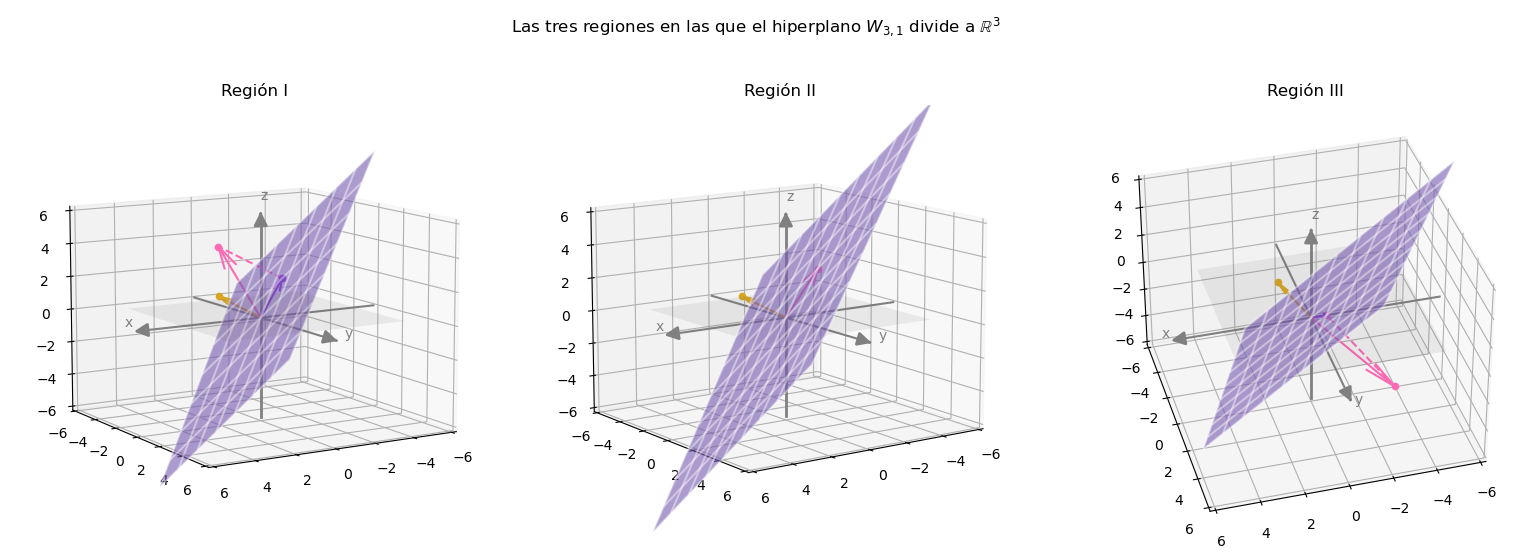
\includegraphics[scale=0.85]{2Dic_4} 
		\caption{Se ilustran las tres 
		regiones en las que $W_{3,1} \subseteq \IR^{3}$ divide al espacio,
		clasificadas según el signo que tome 
		la función $\varphi$ como se definió en
		\eqref{eq: funcion phi ejemplo}. En
		{\color{ameDorado}{dorado}} se muestra al vector
		$\cali{L}^{3,2}$, en {\color{ameRosa}{rosa}}
		un elemento de la región citada, y en 
		{\color{ameMorado}{morado}} la proyección de este
		al espacio $W_{3,1}$.
		}
 	\end{measuredfigure}
 \end{figure}

Es fácil obtener una expresión para el coseno del ángulo
$\alpha$ en términos de los coeficientes de $x$ respecto a $\cali{L}^{3}$:

\begin{figure}[H]
\centering\captionsetup{format = hang}
	\begin{measuredfigure}
		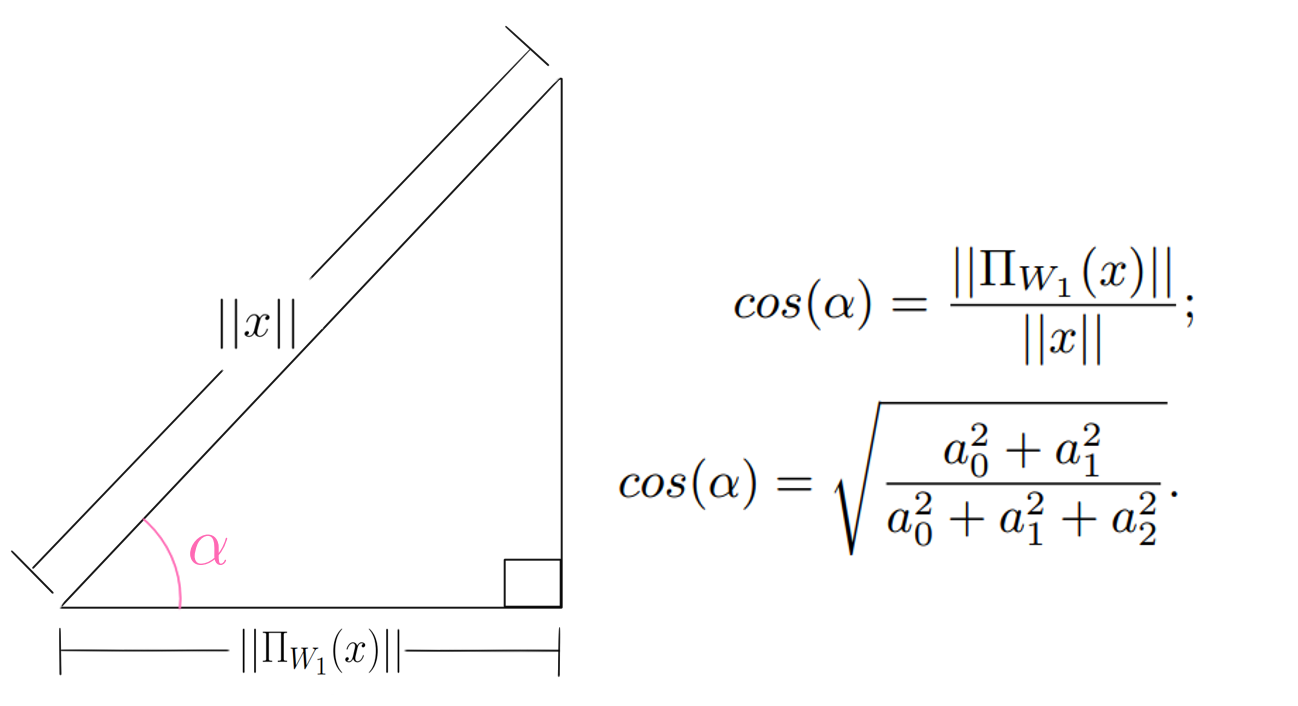
\includegraphics[scale=0.7]{2Dic_3} 
		\caption{\TODO{por qué ese ángulo era recto?}}
 	\end{measuredfigure}
 \end{figure}

De las relaciones de la figura \TODO{ref}
obtenemos una igualdad que relaciona el ángulo 
$\alpha$ que forma una señal $x \in \IR^{3}$ 
con su proyección al espacio $W_{3,1}$
con los coeficientes $a_{i}$
de $x$ respecto a $\cali{L}^{3}$:
\begin{equation}
\label{eq0: 3Dic}
cos(\alpha)= \sqrt{\frac{a_{0}^{2}+a_{1}^{2}}{a_{0}^{2}+a_{1}^{2}+a_{2}^{2}}}.
\end{equation}

Para un ejemplo aún más concreto, hagamos 
\begin{equation}
\label{eq1: 19Sept}
a_{0}= \sqrt{3}, \hspace{0.2cm} a_{1}= \sqrt{2},
\end{equation}



es decir, consideremos a todos los vectores de $\IR^{3}$
cuya proyección al plano $W_{3,1}$ es 
el vector
\begin{equation}
\label{eq1: 6Dic}
(0,1,2).
\end{equation}
Es obvio que el conjunto de los puntos
del espacio cuyas proyecciones a 
$W_{3,1}$ es \eqref{eq1: 6Dic} de hecho es la recta
con ecuación vectorial
\begin{equation}
\label{eq0: 6Dic}
l_{(0,1,2)} := (0,1,2)+c(1,-2,1), \hspace{0.2cm} c \in \IR.
\end{equation}

Sustituyendo
los valores \eqref{eq1: 19Sept} en \eqref{eq0: 3Dic} y
despejando, obtenemos 
\[
|a_{2}|= \sqrt{5 tg^{2}(\alpha)};
\]
el signo del coeficiente $a_{2}$ (que corresponde a la dirección
de $\cali{L}^{3,2}$ en la descomposición de $x$) se determina por
la región en la que se encuentre $x$;

\begin{itemize}
\item el signo de $a_{2}$ es positivo si $x$ es elemento de la región I,
\item $a_{2}=0$ si $x$ es elemento de la región II, y
\item el signo de $a_{2}$ es negativo si $x$ es elemento de la región III.
\end{itemize}


Grafiquemos ahora algunos elementos
de la recta \eqref{eq0: 6Dic}; en los pies
de la figura se especifica el ángulo
$\alpha$ que forma con su proyección así
como la región del espacio a la que pertenece.
Los valores de las entradas de $x$, en la
mayoría de los casos, han sido redondeados.
\end{itemize}
\begin{figure}[H]
\centering\captionsetup{format = hang}
	\begin{measuredfigure}
		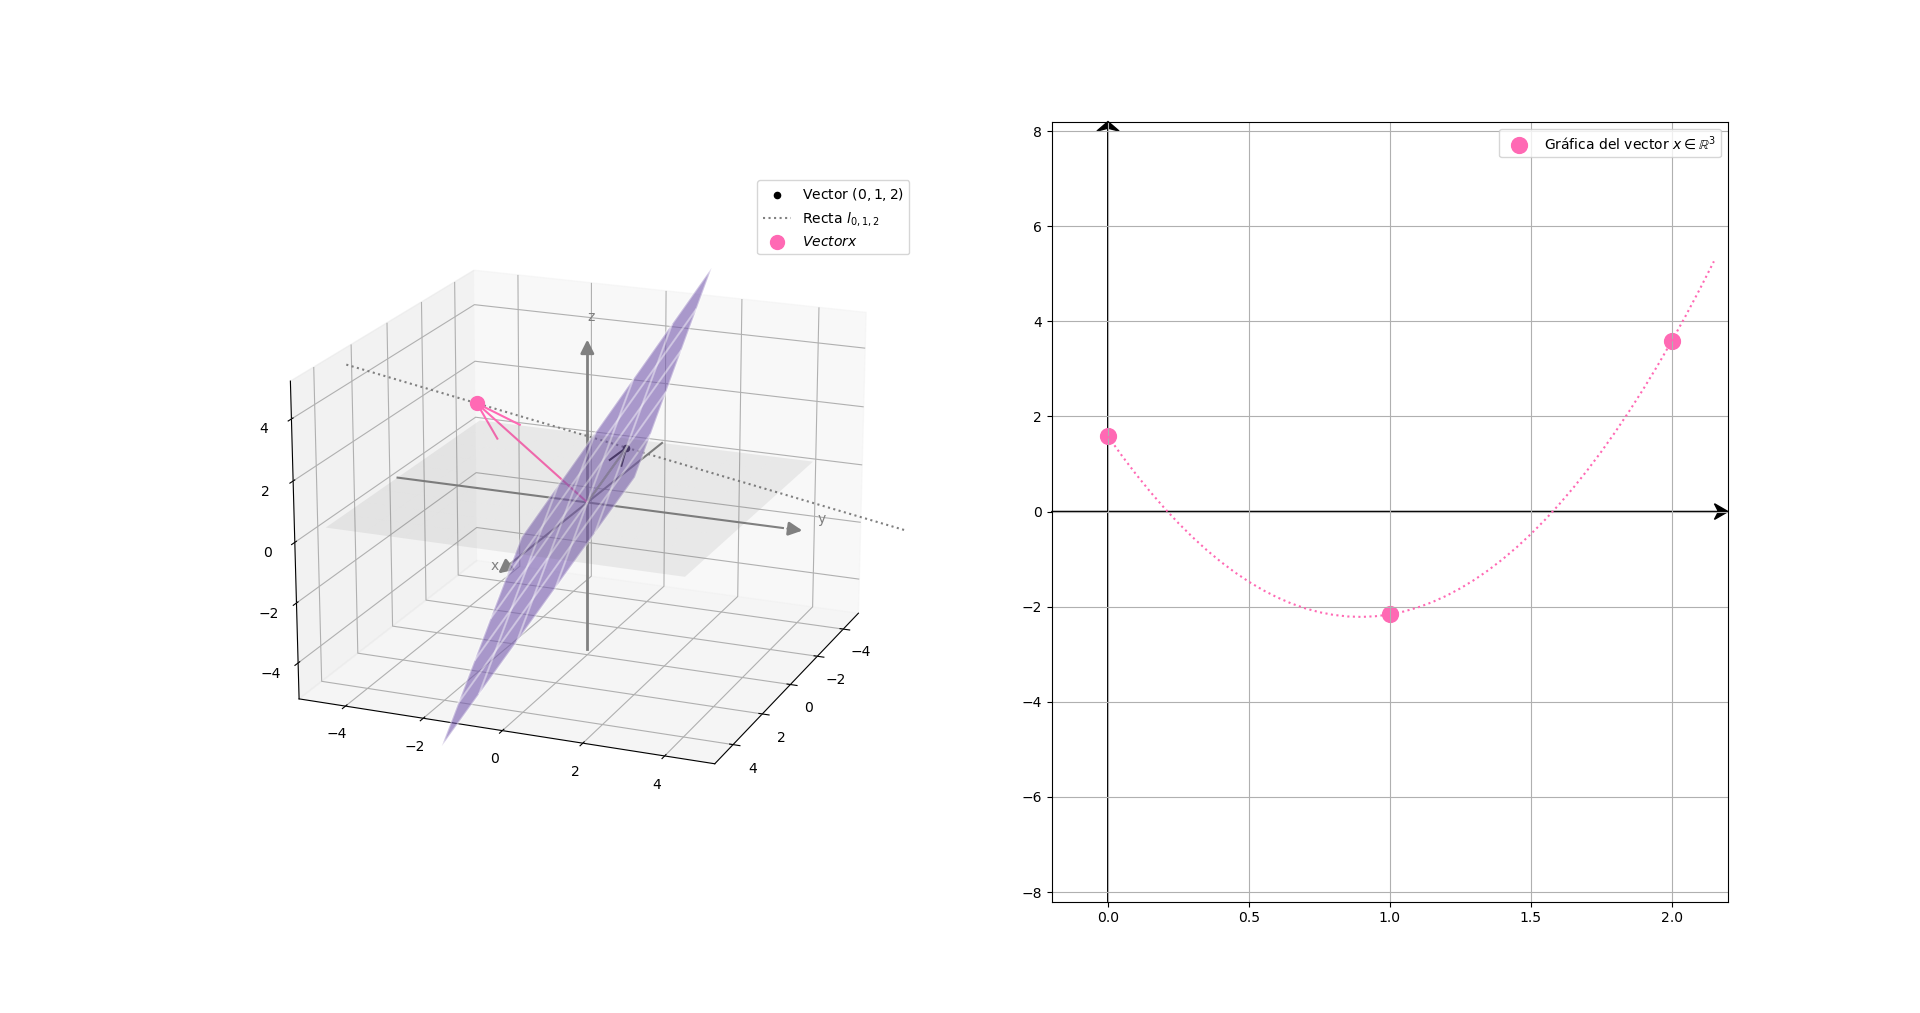
\includegraphics[scale=0.33]{6Dic_0} 
		\caption{Aquí se considera al vector 
		$x=(1.58, -2.16,3.58)$ que forma un ángulo $\alpha=\pi/3$
		con el plano $W_{3,1}$ y que se ubica en la región I.
		\TODO{te faltó graficar al vector normal L3,2.}}
 	\end{measuredfigure}
 \end{figure}


\begin{figure}[H]
\centering\captionsetup{format = hang}
	\begin{measuredfigure}
		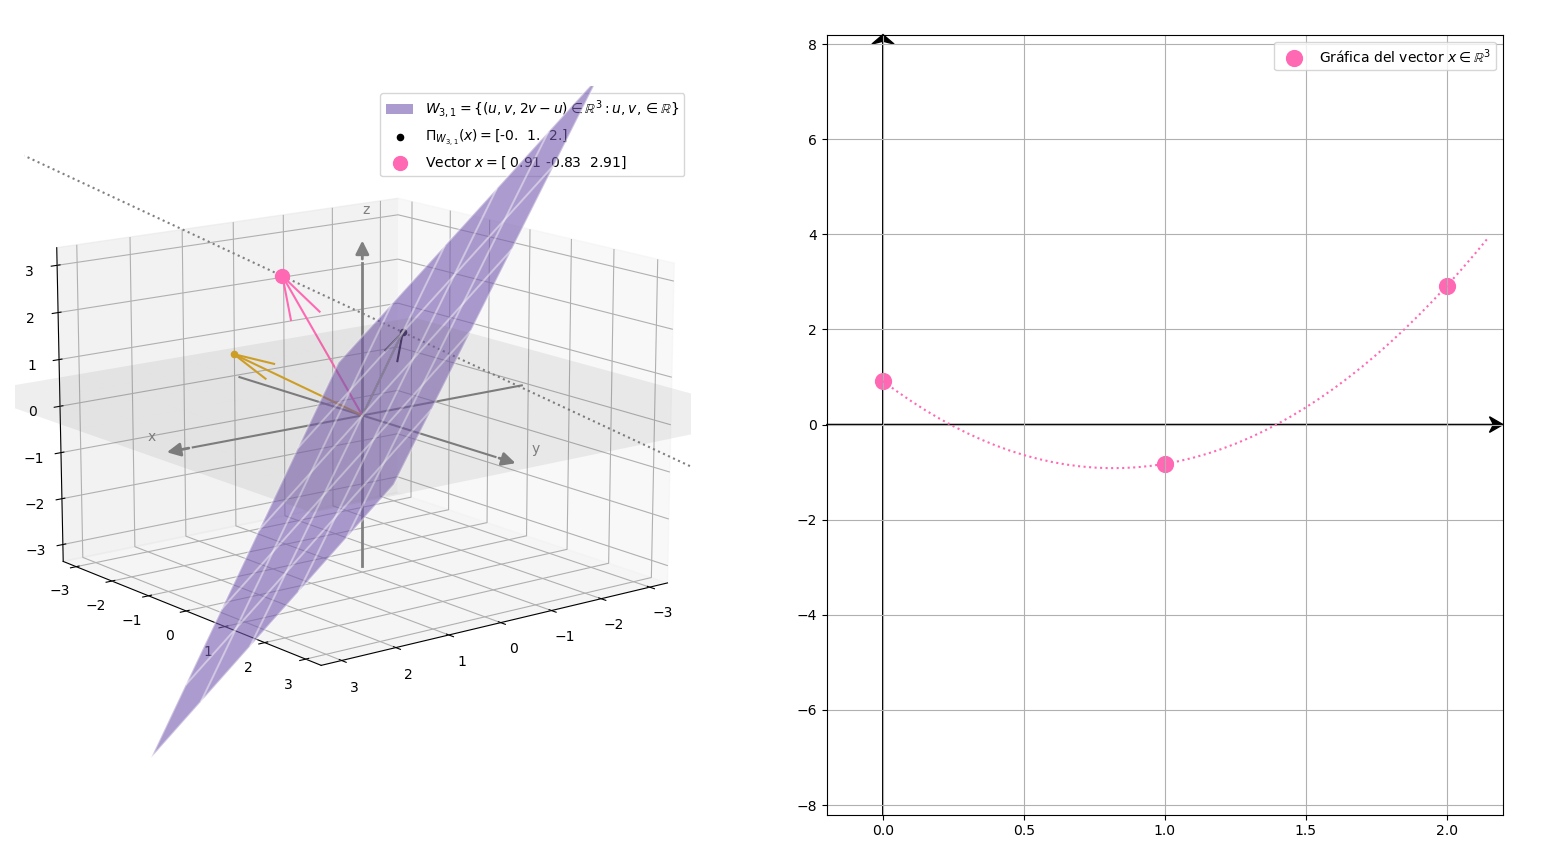
\includegraphics[scale=0.33]{6Dic_1} 
		\caption{Aquí se considera al vector 
		$x=(0.91,-0.82,2.91)$ que forma un ángulo $\alpha=\pi/4$
		con el plano $W_{3,1}$ y que se ubica en la región I.}
 	\end{measuredfigure}
 \end{figure}
 
 
\begin{figure}[H]
\centering\captionsetup{format = hang}
	\begin{measuredfigure}
		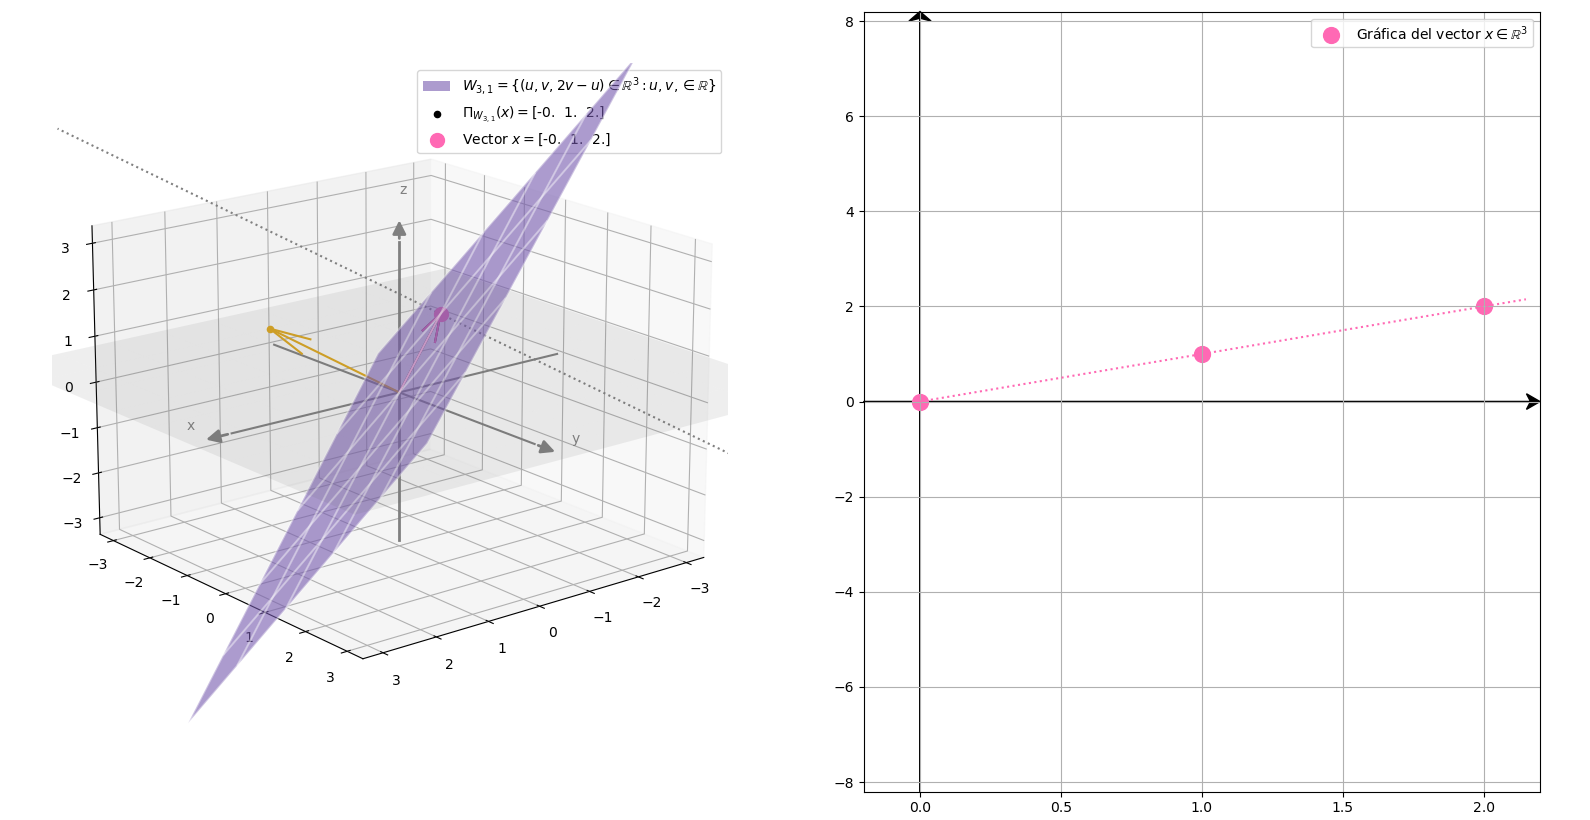
\includegraphics[scale=0.33]{6Dic_2} 
		\caption{Aquí se considera al vector 
		$x=(0,1,2)$ que forma un ángulo $\alpha=0$
		con el plano $W_{3,1}$ y que se ubica en la región II.}
 	\end{measuredfigure}
 \end{figure}

\begin{figure}[H]
\centering\captionsetup{format = hang}
	\begin{measuredfigure}
		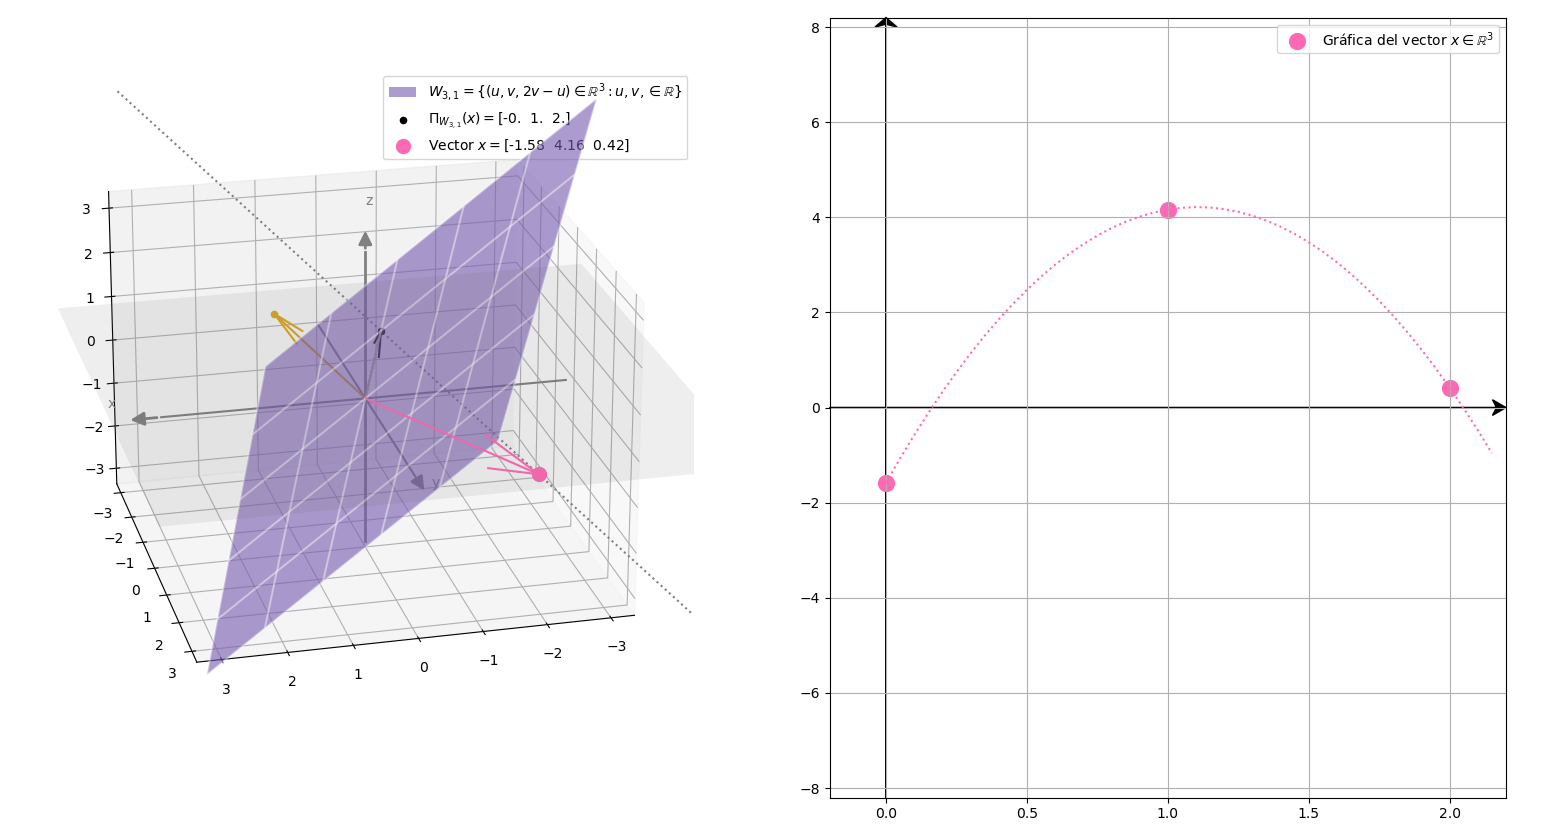
\includegraphics[scale=0.33]{6Dic_3} 
		\caption{Aquí se considera al vector
		$x=(-1.58,4.16,0.41)$ que forma un ángulo $\alpha=\pi/3$
		con el plano $W_{3,1}$ y que se ubica en la región III.}
 	\end{measuredfigure}
 \end{figure}
 
 
\begin{figure}[H]
\centering\captionsetup{format = hang}
	\begin{measuredfigure}
		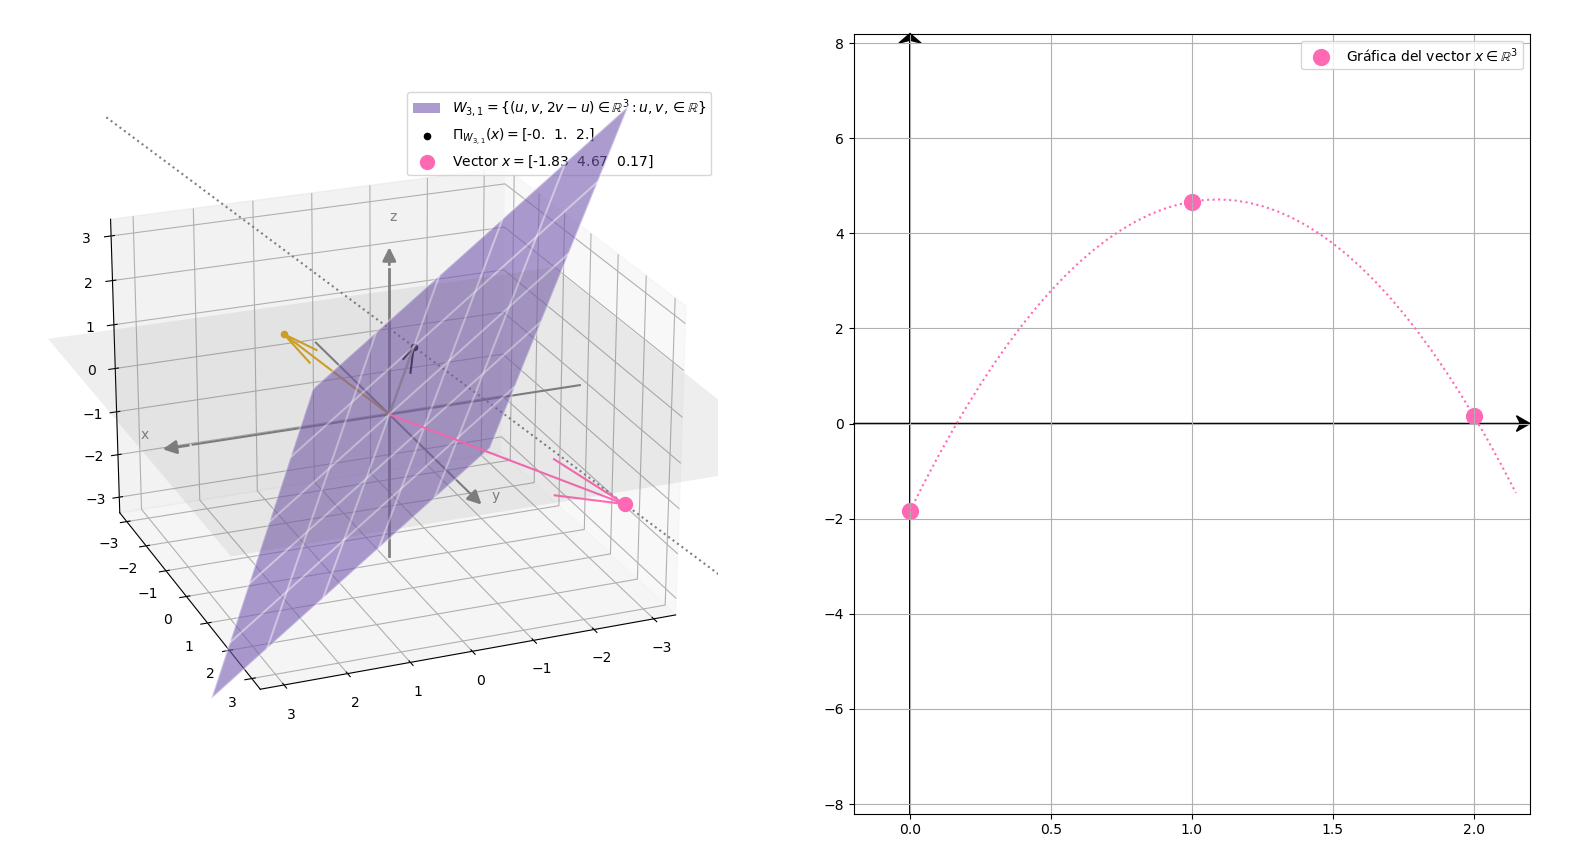
\includegraphics[scale=0.33]{6Dic_4} 
		\caption{Aquí se considera al vector 
		$x=(-1.83,4.66,0.16)$ que forma un ángulo $\alpha=6\pi/17$
		con el plano $W_{3,1}$ y que se ubica en la región III.}
 	\end{measuredfigure}
 \end{figure}
 
 

Veamos por qué, en realidad, la alternativa $b)$
descrita arriba es mucho mejor que la $a)$ para cuantificar 
la morfología de una señal finita.

Si $x \in \IR^{n}$ es una señal de dimensión $n$ y 
$\lambda \in \IR-\{ 0 \}$ es un escalar cualquiera,
la gráfica de $\lambda x$ no es más que la gráfica 
de $x$ reescalada por un factor de $\lambda$ cuando este
último es positivo; en caso contrario, es la gráfica
de $x$ reescalada pero además reflejada respecto al eje
horizontal.


\final
\end{ejemplo}
%Final ejemplo 3--------------------------------------------
 %Sí compila
\section{Sobre formas alternativas de definición de la base $\cali{L}^{n}$}

Ahora,
fijada una dimensión $n$,
vamos a generalizar los tipos de objetos
usados
en el método por medio del cual
se definió a la base de Legendre discreta $\cali{L}^{n}$
(en la subsección 
\ref{Generalización que involucra a la discretización Omega n}),
y además, como prometimos en la introducción,
vamos a dar una segunda forma natural de
de abordar el problema, cambiando el método de 
discretización
(en la subsección 
\ref{Construcción de Ln en base a discretizaciones con sumas integrales}),
llegando, como se anticipó, a la base
$\cali{L}^{n}$.

\subsection{Generalización que involucra a la discretización $\Omega_{n}$}
\label{Generalización que involucra a la discretización Omega n}

Recuerde que, al definir a los espacios
de polinomios discretos
$W_{n,i}$ en \eqref{def de espacios Wk},
consideramos a
las funciones polinomiales 
$f_{k}(t)=t^{k}$, con $0 \leq k \leq n-1$, que después
discretizamos en la malla uniforme
$\cali{P}_{n}= \{ j: \hspace{0.1cm} 0 \leq j \leq n-1 \} $
para obtener los vectores $v_{k}$; nos
disponemos a probar que, si hubiésemos escogido
\begin{itemize}
\item funciones polinomiales
\[
g_{k}(t) \in \IR[x], \hspace{1cm} 
\text{con }\hspace{0.5cm} 0 \leq k \leq n-1 \hspace{0.2cm} \text{entero},
\]
donde
el grado de $g_{k}$ es $k$ y su coeficiente principal 
$c_{k}$ es positivo, y

\item cualquier malla uniforme de $n$ puntos
\[
\cali{P}=\{t_{j} : \hspace{0.1cm} 0 \leq j \leq n-1 \},
\]
\end{itemize}
si 
\begin{equation}
\label{eq1: 31Oct}
w_{k} := \Omega_{n,\cali{P}}(g_{k})
=(g_{k}(t_{j}))_{j=0}^{n-1}, \hspace{0.3cm} 0 \leq k \leq n-1,
\end{equation}
entonces estos vectores $w_{k}$
generan a los mismos espacios $W_{n,i}$
de antes y,
después de ortonormalizar con el 
método de Gram-Schmidt
al subconjunto $\{w_{k}: \hspace{0.2cm} 0 \leq k \leq n-1\}$
de $\IR^{n}$, obtendríamos la 
base de Legendre discreta $\cali{L}^{n}$ 
definida en \eqref{eq: base de Legendre discreta}. 



\begin{ej}
Sea $n=3$; sean las colecciones de polinomios
\begin{equation}
\label{eq11: 10Dic}
\{
f_{0}(t), 
f_{1}(t), f_{2}(t) \},
\end{equation}
con los polinomios $f_{k}$ como se definieron en \eqref{fk}, y
\begin{equation}
\label{eq12: 10Dic}
\left\{
g_{0}(t):=3,  
g_{1}(t):=\frac{1}{2}t+1,
g_{2}(t):=t^{2}+2t+3 \right\}.
\end{equation}



\begin{figure}[H]
\centering\captionsetup{format = hang}
	\begin{measuredfigure}
		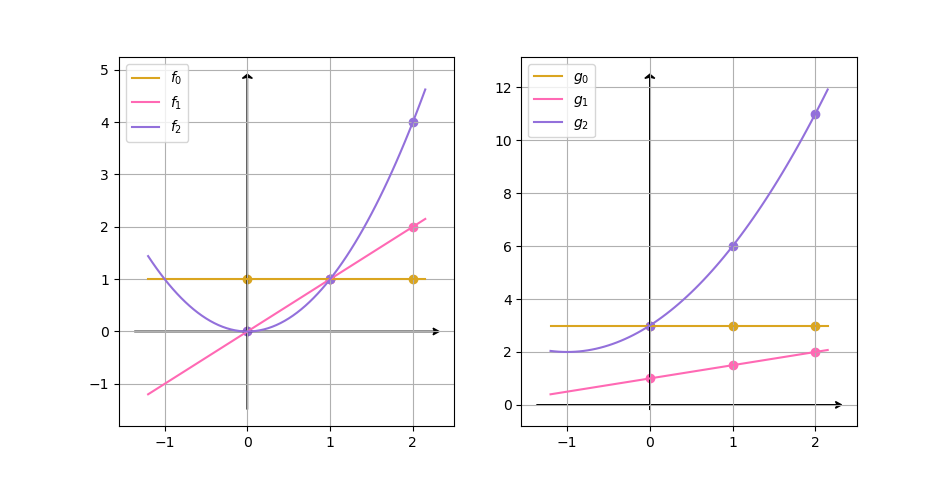
\includegraphics[scale=0.6]{EsquemaGral} 
		\caption{Ejemplo concreto del proceso tomando 
		las dos colecciones
    de polinomios \eqref{eq11: 10Dic} y \eqref{eq12: 10Dic},
    (que tienen en común que contienen, por cada $0 \leq k \leq 2$,
    un polinomio de grado $k$ y coeficiente principal positivo), y
    discretizándolas, respectivamente, en las mallas uniformes 
    $\cali{P}_{3}$ y $\cali{P} =\{-2, -\frac{1}{2}, 1 \}$.}
 	\end{measuredfigure}
 \end{figure}


Afirmamos que, si
\begin{itemize}
\item \textcolor{ameMorado}{{(Discretización)}}
consideramos, para $0 \leq k \leq 2$, a los vectores
\[
v_{k}:= \Om_{3, \cali{P}_{3}}(f_{k})
\hspace{0.2cm} \text{y} \hspace{0.2cm}
w_{k}:= \Om_{3, \cali{P}}(g_{k}),
\]
\item \textcolor{ameMorado}{{(Ortogonalización)}}
en base a estos definimos a los vectores
$$ \bar{\xi}_{0}:= v_{0}, 
\hspace{0.2cm} \bar{\eta}_{0}:= w_{0}, 
$$
$$ \bar{\xi}_{k}:= v_{k} - \Pi_{W_{k-1}}(v_{k}), \hspace{0.2cm}
\bar{\eta}_{k}:= w_{k} - \Pi_{W_{k-1}}(w_{k})
\hspace{0.2cm} \text{para} 
\hspace{0.1cm}
k=1,2, $$ y, finalmente, 
\item \textcolor{ameMorado}{{(Normalización)}}
definimos, para toda $0 \leq k \leq 2$,
a los vectores
$$\xi_{k}:= \frac{\bar{\xi}_{k}}{|| \bar{\xi}_{k} ||},
\hspace{0.2cm}
\eta_{k}:= \frac{\bar{\eta}_{k}}{|| \bar{\eta}_{k} ||},
$$
\end{itemize}
entonces, ocurre que
\[
\forall \hspace{0.1cm} 0 \leq k \leq 2:
\hspace{0.2cm} \xi_{k}= \eta_{k}.
\]
\final
\end{ej}



%\begin{tcolorbox}[title=Ejemplo]

%	\begin{figure}[H]
%	\centering
%	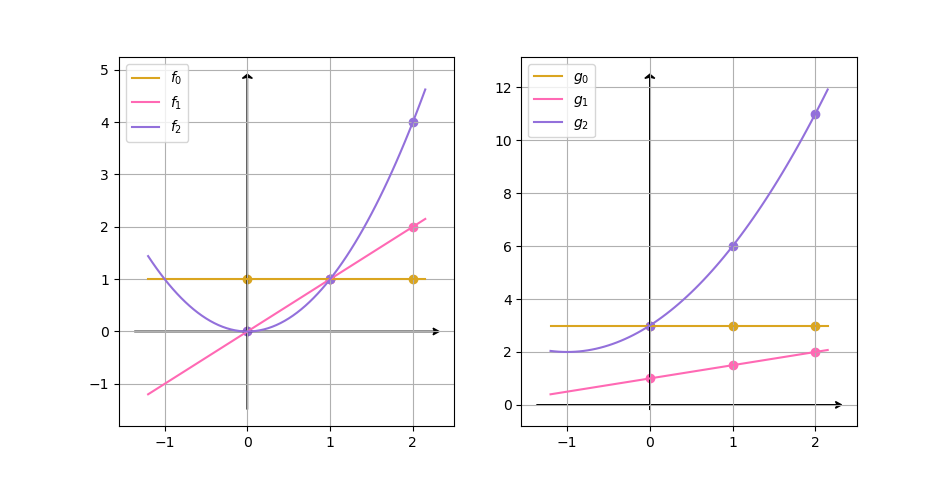
\includegraphics[scale=0.45]{EsquemaGral}
%	\caption{Ejemplo concreto del proceso tomando dos colecciones
 %   de polinomios (a saber, $f_{0}$,  $f_{1}$, $f_{2}$,
  %  y $g_{0}(t):=3$, $g_{1}(t):=\frac{1}{2}t+1$, $g_{2}(t):=t^{2}+2t+3$)
 %   discretizándolas, respectivamente, en las mallas uniformes 
 %   $\cali{P}_{3}$ y $\cali{P} =\{-2, -\frac{1}{2}, 1 \}$.}
%	\end{figure}	

%\tcblower
%\begin{center}
%1.- Discretización
%\end{center}
%\begin{tcbitemize}[raster equal height,colframe=white,colback=white,
%raster every box/.style={minimum for current equal height group=2cm}]
%\tcbitem Consideramos a los vectores
%$$v_{k}:= \Om_{3, \cali{P}_{3}}(f_{k}),$$ con
%$k=0,1,2$.
%\tcbitem Consideramos a los vectores
%$$w_{k}:= \Om_{3, \cali{P}}(g_{k}),$$ con
%$k=0,1,2$.
%\end{tcbitemize}

%\DrawLine

%\begin{center}
%2.- Gram-Schmidt
%\end{center}
%\begin{tcbitemize}[raster equal height,colframe=white,colback=white,
%raster every box/.style={minimum for current equal height group=2cm}]
%\tcbitem Definimos a los vectores
%$$ \bar{\xi}_{0}:= v_{0}, $$
%$$ \bar{\xi}_{k}:= v_{k} - \Pi_{W_{k-1}}(v_{k}),
%\hspace{0.2cm} k=1,2. $$

%\tcbitem Definimos a los vectores
%$$ \bar{\eta}_{0}:= w_{0}, $$
%$$ \bar{\eta}_{k}:= w_{k} - \Pi_{W_{k-1}}(w_{k}),
%\hspace{0.2cm} k=1,2. $$
%\end{tcbitemize}


%\DrawLine

%\begin{center}
%3.- Normalización
%\end{center}
%\begin{tcbitemize}[raster equal height,colframe=white,colback=white,
%raster every box/.style={minimum for current equal height group=2cm}]
%\tcbitem Definimos a los vectores
%$$ \xi_{k}:= \frac{\bar{\xi}_{k}}{|| \bar{\xi}_{k} ||},
%\hspace{0.2cm} k=0,1,2. $$

%\tcbitem Definimos a los vectores
%$$ \eta_{k}:= \frac{\bar{\eta}_{k}}{|| \bar{\eta}_{k} ||},
%\hspace{0.2cm} k=0,1,2. $$
%\end{tcbitemize}
%\DrawLine
%\begin{center}
%Afirmación
%\end{center}
%\begin{tcolorbox}[use height from group=C,add to height=-2cm,
%colframe=white,colback=white]
%\begin{center}
%$\forall \hspace{0.1cm} 0 \leq k \leq 2: \hspace{0.2cm} \xi_{k}=\eta_{k}$.
%\end{center}
%\end{tcolorbox}
%\end{tcolorbox}







\begin{itemize}
\item[\textbf{Paso I}] 
Primero demostremos que vectores $w_{k}$ así
construidos forman bases para los espacios
de polinomios discretos.
\begin{prop}
\label{prop: los wk forman bases de los Wnk}
Sea 
\begin{equation}
\label{eq5: 2En}
\{g_{k}: \hspace{0.2cm} 0 \leq k \leq n-1 \} 
\end{equation}
una colección
de polinomios, con $g_{k}$ un polinomio de grado $k$ y coeficiente 
principal positivo. Sean 
$\cali{P}$ una malla uniforme de $n$ puntos y 
considere a los vectores $w_{k}$ 
definidos en \eqref{eq1: 31Oct}.
Para toda $0 \leq i \leq n-1$, los vectores
\[
w_{k} \hspace{0.2cm} \text{con } 0 \leq k \leq i
\]
conforman una base del espacio $W_{n,i}$.
\end{prop}
\noindent
\textbf{Demostración.}
Observe que el subconjunto \eqref{eq5: 2En}
de $\IR[x]$
es linealmente independiente 
en tal espacio (por cuestión de grados,
ningún $g_{k}$ puede expresarse como combinación lineal de
los anteriores); así, según 
la proposición \ref{Teorema1},
para toda $0 \leq k \leq n-1$, los $n$ vectores $w_{k}$
de $\IR^{n}$ 
definidos en 
\eqref{eq1: 31Oct}
son linealmente independientes en $\IR^{n}$.

Puesto que
los $i+1$ primeros de ellos son elementos del 
espacio $W_{n,i}$
(c.f. proposición \ref{Obs1}) y 
como $dim(W_{n,i})=i+1$
(c.f. teorema \ref{cor: propiedades importantes de espacios Wi}), 
estos $i+1$ vectores conforman
una base del espacio $W_{n,i}$.
\QEDB
\vspace{0.2cm}


\item[\textbf{Paso II}] 
Tenemos entonces dos bases de 
$W_{n,n-1}=\IR^{n}$:
\begin{equation}
\label{eq2: 31Oct}
\{v_{i} : \hspace{0.1cm} 0 \leq i \leq n-1 \} \subseteq \IR^{n}
\hspace{0.25cm} \text{y} \hspace{0.25cm}
\{w_{i} : \hspace{0.1cm}  0 \leq i \leq n-1 \}\subseteq \IR^{n},
\end{equation}

donde, recuerde, los vectores $v_{i}$ se definen como en
\ref{notacion: Pn, fk, Wi, vk}
y los $w_{i}$ son las discretizaciones definidas en
\eqref{eq1: 31Oct}.
Sean
\begin{equation}
\label{eq3: 31Oct}
\{\bar{\xi_{i}}: \hspace{0.1cm}  0 \leq i \leq n-1 \}
\hspace{0.25cm} \text{y} \hspace{0.25cm}
\{\bar{\eta_{i}}: \hspace{0.1cm}  0 \leq i \leq n-1 \}
\end{equation}

las bases que resultan de ortogonalizar a 
las bases dadas en \eqref{eq2: 31Oct} con G-S, y 
\begin{equation}
\label{eq4: 31Oct}
\{\xi_{i}: \hspace{0.1cm} 0 \leq i \leq n-1  \}, \hspace{0.5cm}
\{\eta_{i}: \hspace{0.1cm} 0 \leq i \leq n-1 \}
\end{equation}
a las normalizaciones de las bases dadas en 
\eqref{eq3: 31Oct}, o sea, a las bases cuyos elementos son,
respectivamente,
\begin{equation}
\label{eq0: 1En}
\xi_{i}:= \frac{\overline{\xi_{i}}}{||\overline{\xi_{i}}||}
\hspace{0.5cm} \text{y} \hspace{0.5cm}
\eta_{i}:= \frac{\overline{\eta_{i}}}{||\overline{\eta_{i}}||}
\end{equation}
con $0 \leq i \leq n-1$.

De la definición de los vectores \eqref{eq0: 1En}
y el teorema \eqref{cor: propiedades importantes de espacios Wi} se
sigue inmediantamente lo siguiente:

\begin{obs}
\label{obs: los xi y los etai son elementos de Wni}
Sea $n \in \IN$. Para cada $0 \leq i \leq n-1$, los vectores
$\xi_{i}$ y $\eta_{i}$ 
definidos en \eqref{eq0: 1En} son elementos del
subespacio $W_{n, i}$ de $\IR^{n}$.
\end{obs}

La importancia del \textbf{Paso I} es que, 
para efectuar los dos
procesos de G-S necesarios para
construir las bases 
\eqref{eq3: 31Oct}, a pesar de que trabajaremos
con dos bases distintas de $\IR^{n}$,
vamos a estar proyectando siempre sobre 
los mismos espacios $W_{n,i}$.
Esta observación es clave para la 
demostración de la siguiente proposición.


\begin{prop} \label{prop:signo}
Sea $n \in \IN$.
Para $0 \leq i \leq n-1$, sean los vectores $\xi_{i}$
y $\eta_{i}$ como en \eqref{eq4: 31Oct}.
Para toda $i$, $\xi_{i}= \pm \eta_{i}$.
\end{prop}
\noindent
\textbf{Demostración.}
La clave de la demostración
radicará en ``atrapar'' en un mismo espacio de 
dimensión uno a los vectores
unitarios $\xi_{i}$ y $\eta_{i}$ de $\IR^{n}$. 


Sea $i=0$. Según el teorema de Gram-Schmidt
\ref{Prop:Gram-Schmidt2}, $\overline{\xi_{0}}=v_{0}$
y $\overline{\eta_{0}}=w_{0}$; además,
por definición, $v_{0}$ es
el vector constante uno, y
$w_{0}$ es la discretización (en una malla uniforme $\cali{P}$)
de un polinomio constante $g(t)=c_{0}$ con $c_{0}>0$.
Usando esto y la definición \eqref{eq0: 1En}
tenemos que

\[
\xi_{0}=
\frac{\overline{\xi_{0}}}{||\overline{\xi_{0}}||}=
\frac{v_{0}}{||v_{0}||}=\frac{(1, \ldots , 1)}{\sqrt{n}}=
\frac{(c_{0}, \ldots , c_{0})}{c_{0}\sqrt{n}}= \frac{w_{0}}{||w_{0}||}=
\frac{\overline{\eta_{0}}}{||\overline{\eta_{0}}||}=\eta_{0},
\]
o sea, la veracidad de la proposición para $i=0$.



Sea ahora $1 \leq i \leq n-1$.
Según la definición de los espacios
$W_{n,i}$ dada en \eqref{espacios Wi}
y lo notado en el \textbf{Paso I},
\[
span\{ v_{k}: \hspace{0.1cm} 0 \leq k \leq i \}=W_{n,i}=
span\{ w_{k}: \hspace{0.1cm} 0 \leq k \leq i \},
\]
luego, según la definición de las bases
\eqref{eq4: 31Oct}
el teorema de Gram-Schmidt
\ref{Teo:Gram-Schmidt},

\[
span\{ \xi_{k}: \hspace{0.1cm} 0 \leq k \leq i \}=
W_{n,i} =span\{ \eta_{k}: \hspace{0.1cm} 0 \leq k \leq i \}.
\]
\noindent
Similarmente,
\[
span\{ \xi_{k}: \hspace{0.1cm} 0 \leq k \leq i-1 \}=
W_{n,i-1} =span\{ \eta_{k}: \hspace{0.1cm} 0 \leq k \leq i-1 \}.
\]

Recuerde ahora que el espacio $W_{n,i-1}$
está contenido en $W_{n,i}$
(c.f. teorema \ref{cor: propiedades importantes de espacios Wi});
si por $V_{n,i}$ denotamos al complemento ortogonal de $W_{n,i-1}$
no respecto a $\IR^{n}$, sino 
respecto a $W_{n,i}$, i.e. si
\begin{equation}
\label{eq1: 1En}
V_{n,i} := W_{n,i} \ominus W_{n,i-1},
\end{equation}
entonces, como 
$dim(W_{n,i})=i+1$ y $dim(W_{n,i-1})=i$
(c.f. teorema \ref{cor: propiedades importantes de espacios Wi}), 
$V_{n,i}$ es un espacio
vectorial de dimensión uno
(c.f. \TODO{apéndice,}). Ahora bien,

\begin{itemize}
\item como se notó en la observación 
\ref{obs: los xi y los etai son elementos de Wni},
$\xi_{i}$ es un elemento de $W_{n,i}$ que,
según el teorema de Gram-Schmidt \ref{Teo:Gram-Schmidt},
es ortogonal
a $\xi_{0}, \ldots , \xi_{i-1}$, luego, 
según la ecuación \eqref{eq1: 1En},
$\xi_{i} \in V_{n,i}$.

\item Dualmente, $\eta_{i} \in V_{n,i}$.
\end{itemize}

En conclusión, $\xi_{i}$ y $\eta_{i}$ 
son vectores unitarios ambos pertenecientes al espacio
uno-dimensional $V_{n,i}$; de esto concluimos, como
queríamos, que $\xi_{i} = \pm \eta_{i} $. \QEDB
\vspace{0.2cm}


Del razonamiento de la demostración anterior se sigue una propiedad
importante de los vectores $\xi_{i}$ y $\eta_{i}$,
a saber, su pertenencia a los espacios $V_{n,i}$
definidos en \eqref{eq1: 1En};

\begin{cor} \label{cor: xi y eta ortogonales a elementos de...}
Sea $n \in \IN$.
Para toda $1 \leq i \leq n-1$, los vectores 
$\xi_{i}$ y $\eta_{i}$ definidos en \eqref{eq0: 1En}
son ortogonales a todo polinomio
discreto de dimensión $n$ 
de grado menor a $i$ (i.e. a todo elemento
del espacio $W_{n,k}$ con $k < i$).
\end{cor}




\item[\textbf{Paso III}] Para demostrar que de hecho 
el signo correcto en la
proposición \ref{prop:signo} es siempre positivo, 
será conveniente
establecer antes el siguiente

\begin{lema} \label{Lema1}
Sea $n \in \IN$. 
Para toda
$1 \leq i \leq n-1$, 
sean $w_{i}$ y $\overline{\eta_{i}}$ los vectores
de $\IR^{n}$ definidos como en 
\eqref{eq1: 31Oct} y
\eqref{eq3: 31Oct}.
Los números reales
\[
\langle \bar{\eta}_{i} , w_{i} \rangle \hspace{0.2cm}
\text{y} \hspace{0.2cm} \langle \eta_{i} , w_{i} \rangle 
\]
son ambos positivos.
\end{lema}
\noindent
\textbf{Demostración.}
Puesto que estos números difieren por la multiplicación
de una constante positiva
(a saber, el recíproco de la norma
del vector $\bar{\eta}_{i}$;
recuerde que $\eta_{i}$
se definió como la normalización
del vector $\bar{\eta}_{i}$), basta demostrar que 
ocurre $\langle\bar{\eta}_{i}, w_{i} \rangle >0$. \\
Recuerde que, según la versión del 
teorema de G-S dada en \ref{Prop:Gram-Schmidt2},
\[
w_{i}= \bar{\eta}_{i} + \Pi_{W_{n,i-1}}(w_{i});
\]
puesto que los vectores $\bar{\eta}_{i}$
y $\Pi_{W_{n,i-1}}(w_{i})$ de $\IR^{n}$  son ortogonales entre sí, 
podemos
aplicar la identidad de Parseval (c.f. 
inciso f) del teorema 
\ref{thm: Coway, 4.13})
para establecer la siguiente igualdad en $\IR$:

\[
||w_{i}||^{2} = ||\bar{\eta}_{i}||^{2} + ||\Pi_{W_{n,i-1}}(w_{i})||^{2};
\]
como el vector $\bar{\eta}_{i}$ no es cero (ya lo hemos
exhibido en \eqref{eq3: 31Oct} como elemento de una base de un espacio), de esta
última ecuación obtenemos la desigualdad
\[
||\Pi_{W_{n,i-1}}(w_{i})|| < ||w_{i}||;
\]
multiplicando ambos lados de la desigualdad
por el real positivo $||w_{i}||$ y usando
la desigualdad de Cauchy-Schwarz \ref{Teo:CauchySchwarz},
llegamos a que
\[
\langle w_{i} , \Pi_{W_{n,i-1}}(w_{i}) \rangle \leq 
|\langle w_{i} , \Pi_{W_{n,i-1}}(w_{i}) \rangle|
\leq ||w_{i}|| \cdot 
||\Pi_{W_{n,i-1}}(w_{i})|| < ||w_{i}||^{2},
\]
o sea, a que
\[
||w_{i}||^{2}-\langle w_{i} , \Pi_{W_{n,i-1}}(w_{i}) \rangle >0.
\]

Concluimos gracias a esta desigualdad que
el número real
\begin{align*}
\langle \bar{\eta}_{i} , w_{i} \rangle = &
\langle w_{i}- \Pi_{W_{n,i-1}}(w_{i}), w_{i} \rangle
\\ 
= & \langle w_{i}, w_{i}\rangle - 
\langle 
\Pi_{W_{n,i-1}}(w_{i}),w_{i} \rangle \\
= & ||w_{i}||^{2} - 
\langle w_{i}, \Pi_{W_{n,i-1}}(w_{i}) \rangle
\end{align*}
es mayor a cero.
\QEDB
\vspace{0.2cm}

Estamos listos para demostrar la igualdad 
entre los vectores $\xi_{i}$ y $\eta_{i}$.

\begin{prop} \label{igualdad entre los vectores xi sub i y eta sub i}
Sea $n \in \IN$. Sean 
\begin{equation*}
\{\xi_{i}: \hspace{0.1cm} 0 \leq i \leq n-1 \}, \hspace{0.5cm}
\{\eta_{i}: \hspace{0.1cm} 0 \leq i \leq n-1 \}
\end{equation*}
las colecciones de vectores
definidas en
\eqref{eq4: 31Oct}. Para toda $0 \leq i \leq n-1$,
\[
\xi_{i} = \eta_{i}.
\]
\end{prop}
\noindent
\textbf{Demostración.}
Sea $0 \leq i \leq n-1$ entero. 
Ya vimos en la demostración
de la proposición 
\ref{prop:signo} que $\xi_{0}= \eta_{0}$. 
Según esta misma proposición,
si $i>1$,

\begin{equation}
\label{eq10: 1Nov}
\xi_{i}=a_{i} \eta_{i}, \hspace{0.4cm}
\text{con} \hspace{0.2cm} a_{i} \in \{ \pm 1 \}.
\end{equation}

Si demostramos que $a_{i}$ es positivo, acabamos.
Ahora bien, por ser $\eta_{i}$ un vector unitario,
$\langle\eta_{i} , \eta_{i} \rangle =1$, luego,
como 
\begin{equation}
\label{eq9: 1Nov}
\xi_{i}= d_{i} (v_{i}-\Pi_{W_{n,i-1}}(v_{i})),
\hspace{0.2cm} \text{ con } d_{i}= \frac{1}{||v_{i}-\Pi_{W_{n,i-1}}(v_{i})||},
>0
\end{equation}
tenemos que
\begin{align*}
a_{i} =  a_{i} \langle\eta_{i} , \eta_{i} \rangle &
= \langle a_{i}\eta_{i} , \eta_{i} \rangle \\
(\text{ por \eqref{eq10: 1Nov} }) & = 
\langle \xi_{i} , \eta_{i} \rangle \\
(\text{ por \eqref{eq9: 1Nov} }) & =  
\langle  d_{i} (v_{i}-\Pi_{W_{n,i-1}}(v_{i})), \eta_{i} \rangle \\
& =  d_{i} \left( \langle  v_{i} , \eta_{i} \rangle -
\langle \Pi_{W_{n,i-1}}(v_{i}) , \eta_{i} \rangle  \right) \\
& = d_{i} \langle  v_{i} , \eta_{i} \rangle,
\end{align*}

donde la última igualdad se da por pertenecer la proyección
$\Pi_{W_{n,i-1}}(v_{i})$ al espacio $W_{n,i-1}$ y por ser
$\eta_{i}$,
según el corolario \ref{cor: xi y eta ortogonales a elementos de...},
ortogonal a cualquier elemento de este espacio. \\

Así, $a_{i}$ es el producto del 
real positivo $d_{i}$
con el producto punto
$\langle  v_{i} , \eta_{i} \rangle$,
luego, el signo de $a_{i}$ es el mismo que el de este 
producto punto. 
En este punto del argumento,
nos interesa pues conocer el signo de
$\langle  v_{i} , \eta_{i} \rangle$; como los vectores $\eta_{i}$
se definieron a partir de los vectores $w_{i}$ por el 
proceso de G-S, lo que sí sabemos, gracias al lema
\ref{Lema1}, es que 
\begin{equation}
\label{eq1: 1Nov}
\langle  w_{i} , \eta_{i} \rangle >0.
\end{equation}

Recuerde que, por hipótesis,
$g_{i}$ es un polinomio de grado $i$
con coeficiente principal $c_{i}$ positivo; digamos pues que
$g(x)= \suma{k=0}{i}{c_{k}f_{k}}$,
donde 
\begin{equation}
\label{eq2: 1Nov}
c_{i}>0.
\end{equation}

Según el argumento dado en la demostración de 
la proposición \ref{Obs1}, si 
\begin{equation}
\label{eq3: 1Nov}
h>0
\end{equation} es el paso
de la malla $\cali{P}$, entonces la función
$\phi(t):= ht+t_{0}$ es tal que
\[
\forall \hspace{0.1cm} 0 \leq j \leq n-1: \hspace{0.3cm} t_{j}= \phi(j);
\]
componiendo ambos lados de la igualdad con $g_{i}$
(para alguna $0 \leq i \leq n-1$), llegamos a que

\begin{equation}
\label{eq2: 1En}
\forall \hspace{0.1cm} 0 \leq j \leq n-1: \hspace{0.3cm} g_{i}(t_{j})= G_{i}(j),
\end{equation}
donde

\[
G_{i}(t):= (g_{i} \circ \phi)(t) =
\suma{k=0}{i}{c_{k}(ht+t_{0})^{k}}= c_{i}h^{i}t^{i}+
\suma{k=0}{i-1}{c_{k}(ht+t_{0})^{k}}.
\]
Así, 
\begin{align*}
w_{i}= & (g_{i}(t_{j}))_{j=0}^{n-1} \\ 
\text{(por \eqref{eq2: 1En})} = & (G_{i}(j))_{j=0}^{n-1} \\
= & \left( c_{i}h^{i}j^{i}+
 \suma{k=0}{i-1}{c_{k}(hj+t_{0})^{k}\right)_{j=0}^{n-1}}\\
 = & \left( c_{i}h^{i}j^{i}\right)_{j=0}^{n-1}
 +\left(\suma{k=0}{i-1}{c_{k}(hj+t_{0})^{k}}\right)_{j=0}^{n-1} \\
  = & c_{i}h^{i}\left(j^{i}\right)_{j=0}^{n-1}
 +\left(\suma{k=0}{i-1}{c_{k}(hj+t_{0})^{k}}\right)_{j=0}^{n-1};
\end{align*}
según la notación \ref{notacion: Pn, fk, Wi, vk}, esta
última igualdad puede escribirse como sigue:
\begin{equation}
\label{eq6: 1Nov}
w_{i}= c_{i}h^{i} v_{i}+ z_{i-1},
\end{equation}
donde 
\begin{equation*}
z_{i-1}:=\left(\suma{k=0}{i-1}{c_{k}(hj+t_{0})^{k}}\right)_{j=0}^{n-1};
\end{equation*}
como $z_{i-1}$ es la discretización en una malla uniforme
(a saber, $\cali{P}_{n}$) de un polinomio de grado a lo más $i-1$, 
\begin{equation}
\label{eq4: 1Nov}
z_{i-1} \in W_{n,k} \hspace{0.2cm} \text{ para alguna } k < i;
\end{equation}
según el corolario \ref{cor: xi y eta ortogonales a elementos de...},
la relación \eqref{eq4: 1Nov} implica que
\begin{equation}
\label{eq5: 1Nov}
\langle z_{i-1}, \eta_{i} \rangle =0.
\end{equation}

Despejando a $v_{i}$ de \eqref{eq6: 1Nov}, llegamos a que
\begin{equation}
\label{eq7: 1Nov}
v_{i}= \frac{1}{c_{i}h^{i}} \left( w_{i} -  z_{i-1} \right),
\end{equation}
luego,
\begin{align}
\label{eq8: 1Nov}
\left\langle v_{i}, \eta_{i} \right\rangle = & 
\left\langle \frac{1}{c_{i}h^{i}} \left( w_{i} -  z_{i-1} \right), \eta_{i} 
 \right\rangle \nonumber \\
= & \frac{1}{c_{i}h^{i}} \langle w_{i}, \eta_{i} \rangle -
\frac{1}{c_{i}h^{i}} \langle z_{i-1}, \eta_{i} \rangle \nonumber \\
(\textit{por \eqref{eq5: 1Nov}}) = & \frac{1}{c_{i}h^{i}} \langle w_{i}, \eta_{i} \rangle.
\end{align}
Según 
\eqref{eq2: 1Nov} y 
\eqref{eq3: 1Nov}, $\frac{1}{c_{i}h^{i}}$ es
un número positivo, además, según 
\eqref{eq1: 1Nov}, $\langle w_{i}, \eta_{i} \rangle$ también;
así,\eqref{eq8: 1Nov} expone a $\langle v_{i}, \eta_{i} \rangle$
como el producto de números positivos. 
Concluimos así, como queríamos,
que $\langle v_{i}, \eta_{i} \rangle>0$.
\QEDB
\vspace{0.2cm}


\end{itemize}

\subsection{Construcción de $\cali{L}^{n}$ en base a discretizaciones con sumas integrales}
\label{Construcción de Ln en base a discretizaciones con sumas integrales}
Para terminar la sección de construcciones alternativas
de la base de Legendre,
en esta subsección daremos una segunda
forma natural de discretizar funciones continuas
(esta basada en promedios integrales) a partir de 
la cual, con un proceso análogo al expuesto
en las subsecciones \TODO{ref}, 
construiremos una base del espacio $\IR^{n}$
que, como probaremos, es $\cali{L}^{n}$.



\begin{defi}
(\textbf{Operador de discretización $\Delta_{n,a,b}$})
Dados dos números reales $a<b$, se divide
regularmente al intervalo $[a,b]$ en 
$n$ subintervalos de longitud $h=\frac{b-a}{n}$,
es decir, consideramos la partición

\begin{equation}
\label{eq1: 2En}
\cali{P}_{n}= \{ t_{j} \}_{j=0}^{n}, 
\hspace{0.4cm} \text{con} \hspace{0.2cm}
t_{j}=j\frac{b-a}{n}+a \hspace{0.4cm} \text{para}\hspace{0.4cm}
 0 \leq j \leq n.
\end{equation}
Definimos entonces a la función $\Delta_{n,a,b}$ 
de $\cali{C}[a,b]$ en $\mathbb{R}^{n}$ como
\begin{center}
$\Delta_{n,a,b}(f)= \frac{1}{h} (u_{n,j}(f))_{j=1}^{n},$ \hspace{0.3cm}
$f \in \cali{C}[a,b]$,
\end{center}
donde, para toda $1 \leq j \leq n$,
\begin{center}
$u_{n,j}:= \integ{t_{j-1}}{t_{j}}{f(t)dt}$.
\end{center}
\end{defi}


\begin{figure}[H]
\centering\captionsetup{format = hang}
	\begin{measuredfigure}
		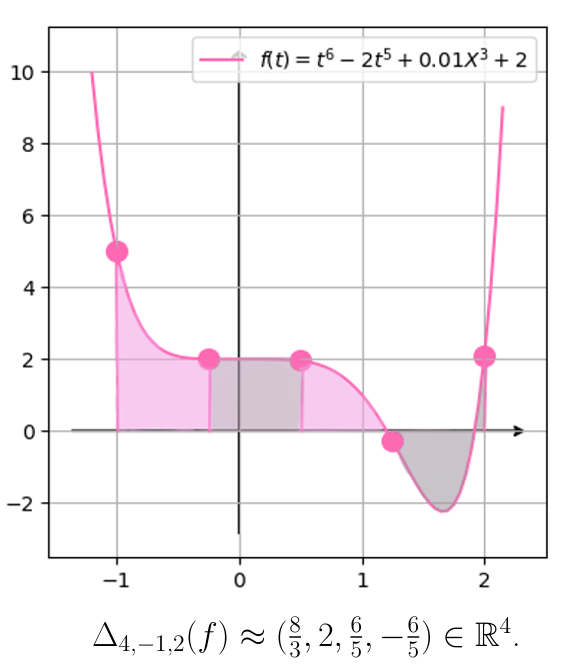
\includegraphics[scale=1.5]{1En_2} 
		\caption{Ejemplo con $n=4$, $a=-1$, $b=2$ y
		$f(t)= t^{6}-2t^{5}+0.01t^{3}+2$}
 	\end{measuredfigure}
 \end{figure}






\noindent
Demostremos que, si escogemos
\begin{itemize}
\item para $0 \leq k \leq n-1$ funciones polinomiales
$g_{k}(t) \in \IR[x]$
\begin{equation}
\label{eq10: 3Nov}
g_{k}(t)= \suma{i=0}{k}{c_{k,i}t^{i}},
\hspace{0.2cm} c_{k, k} >0,
\end{equation}
de grado $k$ y coeficiente principal 
$c_{k,k}$ positivo, 

\item cualquier intervalo $[a,b]$ que partimos 
uniformemente con la malla de $n+1$ puntos
$\cali{P}_{n}= \{ t_{j} \}_{j=0}^{n}$ 
definida en \eqref{eq1: 2En},

\end{itemize}

y si definimos, para toda $0\leq k \leq  n-1$
al vector $u_{k}$ en función de $g_{k}$ como 
\begin{equation}
\label{eq1: 3Nov}
u_{k}:= \Delta_{n,a,b}(g_{k})
= \left( \frac{1}{h} 
\integ{t_{j-1}}{t_{j}}{g_{k}(t)dt} \right)_{j=1}^{n} , 
\end{equation}
entonces los primeros $i$ vectores
de la forma \eqref{eq1: 3Nov}
generan a los espacios $W_{n,i}$
definidos antes en 
\ref{notacion: Pn, fk, Wi, vk},
son linealmente independientes y,
después de ortonormalizarse con 
el proceso de G-S,
obtenemos a los elementos de la base $\cali{L}^{n}$.

Comencemos demostrando la independencia lineal
de los $n$ vectores \eqref{eq1: 3Nov}. Al igual que para
la demostración del resultado análogo 
\ref{Teorema1},
la prueba de este hecho se basa en el teorema
fundamental del álgebra.

\begin{prop}
\label{prop: los uk forman una base de Rn}
Sea $n \in \IN$. El 
subconjunto $\{u_{k} : \hspace{0.1cm} 0 \leq k \leq n-1 \}$
de $\IR^{n}$ , con
$u_{k}$ los $n$ vectores definidos en 
\eqref{eq1: 3Nov},
es linealmente independiente.
\end{prop}
\noindent
\textbf{Demostración.}
Supongamos, por el contrario, 
que existen números reales $a_{k}$, con $0 \leq k \leq n-1$,
no todos cero tales que se tenga la siguiente igualdad en $\IR^{n}$:
\begin{equation}
\label{eq8: 3Nov}
\suma{k=0}{n-1}{a_{k}u_{k}}=0
\end{equation}
Desglosando
la igualdad \eqref{eq8: 3Nov} 
entrada a entrada, descomponemos
a esta en el siguiente sistema de $n$ ecuaciones en $\IR$:
\[
\suma{k=0}{n-1}{ \frac{a_{k}}{h} \int_{t_{j-1}}^{t_{j}}g_{k}(t)\ dt} = 0,
\hspace{0.2cm} 1 \leq j \leq n.
\]
Multiplicando este sistema por $h$, llegamos a las
$n$ igualdades
\begin{equation}
\label{eq2: 2En}
\suma{k=0}{n-1}{a_{k} \int_{t_{j-1}}^{t_{j}}g_{k}(t)\ dt} = 0,
\hspace{0.2cm} 1 \leq j \leq n.
\end{equation}
Por la linealidad de la integral, el sistema \eqref{eq2: 2En}
se reescribe como
\begin{equation}
\label{eq9: 3Nov}
\int_{t_{j-1}}^{t_{j}}p(t)\ dt =0,
\hspace{0.2cm} 1 \leq j \leq n,
\end{equation}


\noindent donde $p$ es el polinomio 
\begin{equation}
\label{eq3: 2En}
p(t):=\suma{k=0}{n-1}{a_{k}g_{k}(t)}. 
\end{equation}
Como todos los polinomios $g_{i}$ son,
por hipótesis, de 
grado menor a $n$ y linealmente independientes
(en el espacio $\IR[x]$),
y se ha supuesto que no
todos los
coeficientes $a_{i}$ son cero, el polinomio
$p$ definido en \eqref{eq3: 2En} es no cero y de grado
menor a $n$. \\

Según el sistema \eqref{eq9: 3Nov}, en cada uno
de los intervalos
\[
I_{j}:=[t_{j-1}, t_{j}], \hspace{0.2cm} 1 \leq j \leq n,
\]

\noindent la función polinomial $p$, continua en todos ellos, 
integra cero. \\

Ahora bien, si en $I_{j}$ la función $p$ fuese siempre
positiva, la integral de esta sería positiva; si fuese
siempre negativa, la integral también
(c.f. \TODO{teorema spivak?}). Existen entonces
puntos $a_{j}$ y $ b_{j}$ en $I_{j}$ tales que
\[
p(a_{j})<0 \hspace{0.2cm} \text{y}
\hspace{0.2cm} p(b_{j})>0.
\]

\noindent Aplicando el teorema del valor intermedio
\TODO{referencia}, 
deducimos la existencia de un 
$r_{j}$ entre $a_{j}$ y 
$b_{j}$ (y que entonces será punto
interior de $I_{j}$) tal que $p(r_{j})=0$;
así, para cada $1 \leq j \leq n$,
hemos
encontrado una raíz $r_{j}$ de $p$ en int($I_{j}$);
por ser ajenos los interiores de los intervalos $I_{j}$,
estamos seguros de que las $n$ raices $r_{j}$ son distintas
entre sí.
Llegamos así
a que el polinomio no cero $p$, cuyo grado es a lo más $n-1$,
tiene al menos $n$ raíces distintas; esto
contradice la proposición \ref{prop: cita TFA}.
\QEDB
\vspace{0.2cm}

\begin{prop}
\label{prop: uk son discretizaciones pol...}
Sean $n \in \IN$. Para toda $0 \leq k\leq n-1$, si
$g_{k} \in \IR[x]$ es como en \eqref{eq10: 3Nov}
y $u_{k} \in \IR^{n}$ como en
\eqref{eq1: 3Nov}, entonces
$u_{k}$ es la discretización en una malla uniforme
de $n$ puntos de un polinomio de grado $k$
y coeficiente principal positivo. En particular,
$u_{k} \in W_{n,k}$.
\end{prop}
\noindent
\textbf{Demostración.}
La $j-$ésima entrada del vector $u_{k}$
(con $1 \leq j \leq n$)
es, según la igualdad \eqref{eq1: 3Nov},

\begin{align} 
\frac{1}{h} \int_{t_{j-1}}^{t_{j}}{g_{k}(t)} \,dt = &
\frac{1}{h} \int_{t_{j-1}}^{t_{j}}{\suma{i=0}{k}{c_{k,i}t^{i}}} \,dt 
\nonumber \\
= & \frac{1}{h} \suma{i=0}{k}{\int_{t_{j-1}}^{t_{j}}{c_{k,i}t^{i}} \, dt}
\nonumber \\
= & \frac{1}{h} \suma{i=0}{k}{
\frac{c_{k,i}}{i+1}t^{i+1} | ^{t=t_{j}}_{t=t_{j-1}}
} 
\nonumber \\
= & \frac{1}{h} \suma{i=0}{k}{
\frac{c_{k,i}}{i+1}t^{i+1} | ^{t=t_{j-1}+\frac{b-a}{n}}_{t=t_{j-1}}} 
\nonumber \\
= & 
\frac{1}{h} \suma{i=0}{k}{
\frac{c_{k,i}}{i+1} \left( t_{j-1}+ \frac{b-a}{n} \right)^{i+1}}-
\frac{1}{h} \suma{i=0}{k}{
\frac{c_{k,i}}{i+1} t_{j-1}^{i+1}}; \nonumber\\
\end{align}
esta última expresión, en principio, es un polinomio
de grado a lo más $k+1$,
que denotaremos por $q_{k}$, evaluado en $t_{j-1}$,
y que está dado por la expresión
\begin{equation} \label{eq2: 5Nov}
q_{k}(t)= \frac{1}{h} \suma{i=0}{k}{
\frac{c_{k,i}}{i+1} \left(t+ \frac{b-a}{n} \right)^{i+1}}-
\frac{1}{h} \suma{i=0}{k}{
\frac{c_{k,i}}{i+1} t^{i+1}}.
\end{equation}

\begin{itemize}
\item Note que las potencias de orden $k+1$ del argumento
$t$ en la expresión \eqref{eq2: 5Nov}
se dan
cuando en la primera y segunda suma el índice $i$
vale $k$; 
tal parte de la suma es 
\begin{equation}
\label{eq1: 5Nov}
\frac{1}{h} \frac{c_{k,k}}{k+1} \left(t+\frac{b-a}{n} \right)^{k+1}-
\frac{1}{h} \frac{c_{k,k}}{k+1} t^{k+1}=
\frac{1}{h} \frac{c_{k,k}}{k+1} t^{k+1}-\frac{1}{h} \frac{c_{k,k}}{k+1} t^{k+1}+ (*)=(*),
\end{equation} 
donde $(*)$ denota un sumando que no contiene potencias de orden
$k+1$ de $t$ (y que, por lo tanto, no interesa para conocer
el coeficiente de $t^{k+1}$).
Así, según \eqref{eq1: 5Nov}, el grado
de $q_{k}$ es a lo más $k$.
\item Busquemos ahora el coeficiente de $q_{k}$ asociado a la
potencia $k$; aparece en
el lado derecho de \eqref{eq2: 5Nov} la potencia $k$
de $t$ cuando en el primer sumando $i=k, k-1$
y también cuando en el segundo sumando $i=k-1$;
así, el coeficiente buscado es
\begin{equation}
\label{eq3: 5Nov}
\frac{1}{h} \frac{c_{k,k}}{k+1}(k+1)\frac{b-a}{n} 
+\frac{1}{h} \frac{c_{k,k-1}}{k}-
\frac{1}{h} \frac{c_{k,k-1}}{k} = 
\frac{1}{h} \frac{c_{k,k}(b-a)}{kn}.
\end{equation}
Puesto que, por hipótesis (c.f. 
condición \eqref{eq10: 3Nov})
el número $c_{k,k}$ es positivo, tenemos que 
el coeficiente principal \ref{eq3: 5Nov}
de $q_{k}$ es positivo.
\end{itemize}


Según todo lo anterior, $u_{k}$
es el polinomio discreto obtenido al evaluar
al polinomio $q_{k}$ (cuyo grado es $k$ y tiene
coeficiente principal \eqref{eq3: 5Nov},
de hecho, es positivo)
en la malla uniforme 
$\cali{P}_{n}=\{t_{j}\}_{j=0}^{n-1}$.
De esto y el teorema 
\ref{cor: propiedades importantes de espacios Wi}
se deduce la pertenecia de $u_{k}$ al espacio $W_{n,k}$.
\QEDB
\vspace{0.2cm}

Recapitulemos; hemos demostrado que 
el subconjunto
\begin{equation}
\label{eq4: 2En}
\{u_{k}: \hspace{0.2cm} 0\leq k \leq n-1 \}
\end{equation}
de $\IR^{n}$
\begin{itemize}
\item es linealmente independiente 
(c.f. proposición \ref{prop: los uk forman una base de Rn}), y que,
\item para toda $0\leq k \leq n-1$, $u_{k}$
es la discretización en una malla uniforme
de $n$ puntos de un polinomio de grado $k$
y coeficiente principal positivo
(c.f. proposición \ref{prop: uk son discretizaciones pol...});
\end{itemize}
así, \eqref{eq4: 2En} es una colección de
polinomios que satisface las condiciones pedidas  
en la subsección
\ref{Generalización que involucra a la discretización Omega n}.
Concluimos, según lo demostrado en esa subsección, 
que el resultado de ortonormalizar la 
base $\{u_{k}\}_{k=0}^{n-1}$ de $\IR^{n}$
(construida, recuerde, a partir del operador de 
discretización $\Delta_{n, a, b}$)
es nuestra base de Legendre
discreta definida en 
\ref{def: base de Legendre discreta}.

\begin{figure}[H]
\centering\captionsetup{format = hang}
	\begin{measuredfigure}
		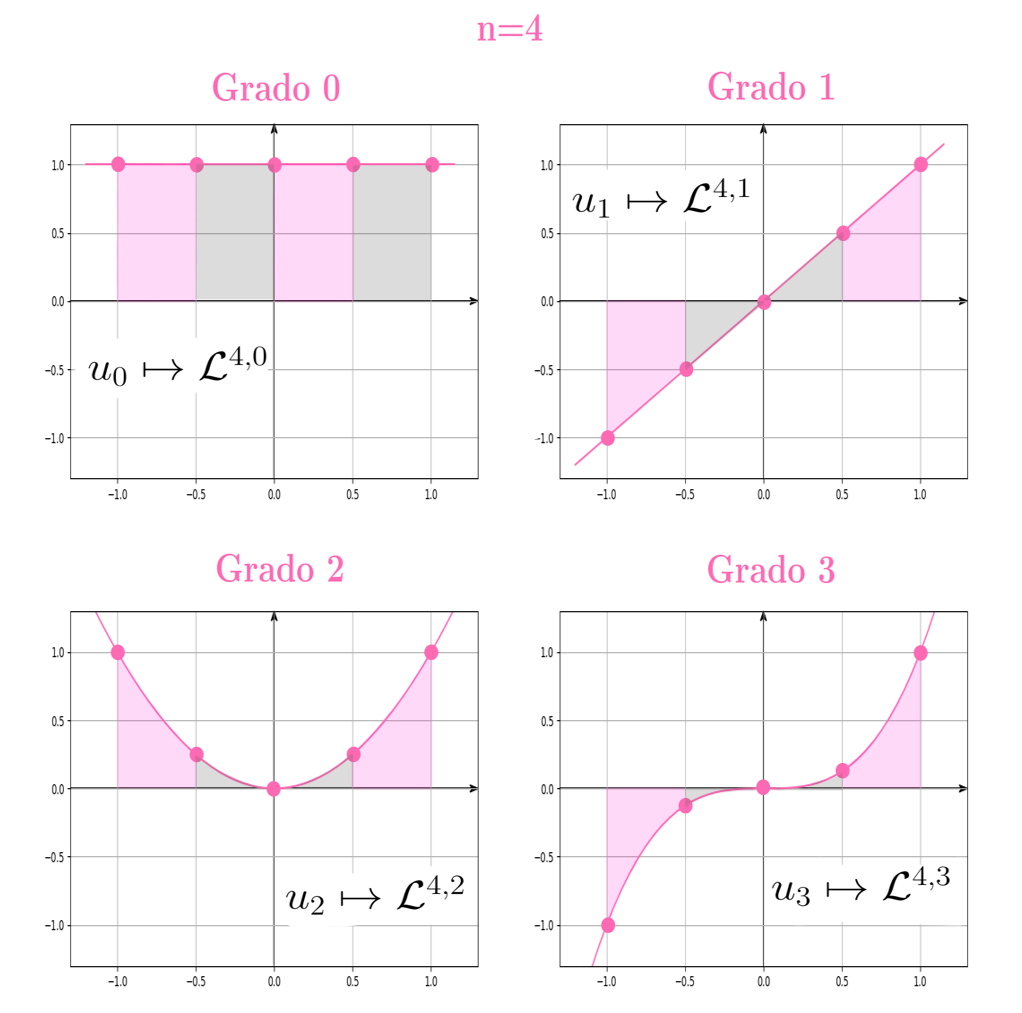
\includegraphics[scale=0.4]{5Dic_1} 
	\caption{Al comenzar este
	trabajo de tesis,
	nuestra definición original de la base $\cali{L}^{n}$
	consistía en discretizar a los polinomios
	$f_{k}$, $0 \leq k \leq n-1$ con el operador $\Delta_{n,-1,1}$.
	En la figura se ilustra este proceso para cuando $n=4$.}
 	\end{measuredfigure}
 \end{figure}
        
     
    
    
\begin{figure}[H]
\centering\captionsetup{format = hang}
	\begin{measuredfigure}
		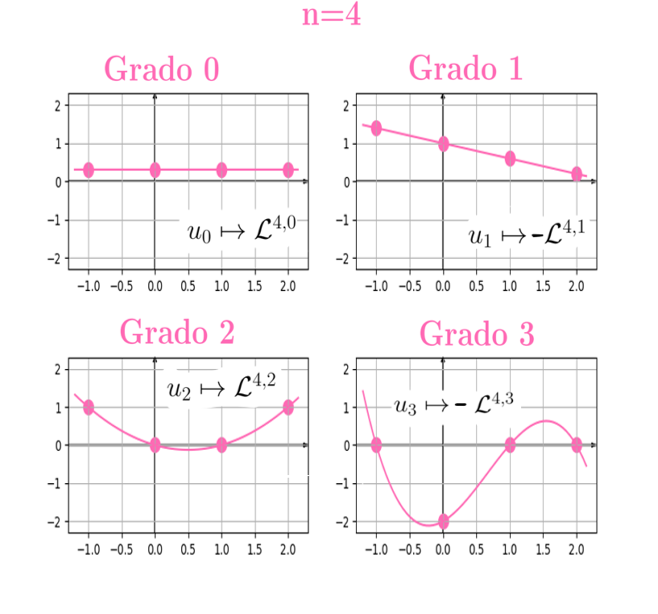
\includegraphics[scale=0.71]{5Dic_2} 
		\caption{Según la teoría
		 desarrollada en esta sección, 
		 fijada una dimensión $n$, podemos
	cambiar tanto la malla uniforme como el método 
	de discretización; después
	de ortonormalizar, salvo por cambios de signo,
	obtendremos a la
	base $\cali{L}^{n}$. 
	Es el coeficiente principal del polinomio
	discretizado para obtener al vector $v_{k}$ 
	el que determina
	el signo correcto. Para el ejemplo mostrado
	en la imagen (donde se ha fijado $n=4$), se
	han considerado a los polinomios
	$h_{0}(t)=0.3$, $h_{1}(t)=-0.4t+1$,
	$h_{2}(t)=0.25t^{2}-0.5t$ y $h_{3}(t)=-t^{3}+2t^{2}+t-2$.
	Como se destaca, los polinomios con coeficiente principal
	negativo (en este caso, los de grados $1$ y $3$)
	dan lugar a los respectivos polinomios de Legendre
	discretos con signo negativo.}
 	\end{measuredfigure}
 \end{figure}
 %Sí compila
\section{Comentarios finales sobre la construcción} 
\label{sec: commentarios finales}
Nuestro primer intento de 
construcción de lo que ahora llamamos 
``base de Legendre discreta'' de dimensión $n$,
y que denotamos por
$\cali{L}^{n}$, se basó en 
un caso particular del punto de vista
dado en la subsección 
\ref{Construcción de Ln en base a discretizaciones con sumas integrales}
(discretizando con el operador $\Delta_{n,a,b}$
a las potencias $f_{k}$
con $0 \leq k \leq n-1$
en el intervalo $[-1,1]$); es la clara analogía 
entre nuestra construcción discreta y la continua
de los polinomios de Legendre (\TODO{aquí
referencia}) una de las
razones por la que acuñamos el nombre para
la BON $\cali{L}^{n}$. \\ 

La determinación de expresiones analíticas para los
elementos de $\cali{L}^{n}$ se hará después de la sección
de revisión de literatura, pues para la tarea haremos uso de las 
fórmulas ofrecidas en uno de los artículos consultados. \\

Para terminar, mencionamos que fue en dicho artículo
(el ~\cite{Neuman})
en donde conocimos el término de ``polinomio dicreto''
(como fue dado en la definición \ref{def: polinomio discreto});
aunque parece una pequeñez, el considerar que
un vector de $\IR^{n}$ fue construido a partir
de la discretización de un polinomio fue de gran importancia
para la generalización de la construcción de la base de Legendre
(que se basó, principalmente,
en identificar la importancia de
los espacios $W_{n,i}$ y usarlos para definir
a los polinomios de Legendre),
pues asociada a la noción de \textbf{polinomio} está la de \textbf{grado}; 
en nuestro
contexto, a esta última noción está ligada la de \textbf{pertenencia a
algún espacio $W_{n,k}$}, y a esta \textbf{criterios sobre la forma de la
gráfica de una señal}
de dimensión $ns$, que es, en principio, lo que nos interesa estudiar.



%%\section{Revisión de literatura y artículos relacionados}

Hicimos una búsqueda en la literatura
para saber si bases parecidas a la
de Legendre discreta
(i.e. a la definida en 
\ref{def: base de Legendre discreta})
ya habían sido 
consideradas antes y, en caso afirmativo, las propiedades
conocidas sobre ellas. 


\begin{itemize}
\item Encontramos el artículo \textit{``Discrete (Legendre) 
orthogonal polynomials -a survey''} ~\cite{Neuman}, en el que se habla de
ciertos polinomios ortogonales de variable independiente
discreta; fijado un entero $n$,
se afirma (pero no demuestra) la existencia de únicas funciones
\[
P_{k}(\cdot ,n)=P_{k}(m,n), \hspace{1cm} 0 \leq k \leq n
\]
de variable discreta $0 \leq m \leq n $, tales que


\begin{equation}
\suma{m=0}{n}{P_{k}(m,n) P_{l}(m,n)} =0
\hspace{0.3cm} \text{si} \hspace{0.2cm} m \neq l \tag{DLOP-1[n]} \label{eq:dlop1}
\end{equation}
y 
\begin{equation}
\text{para toda} \hspace{0.3cm} 0 \leq k \leq n, \hspace{0.3cm} P_{k}(0, n)=1.   \tag{DLOP-2[n]} \label{eq:dlop2}
\end{equation}


Pensando en los 
$n+1$ vectores de $\IR^{n+1}$ que resultan
de evaluar estas funciones discretas en su rango,
es decir, en los vectores
\begin{equation}
y_{k}:= (P_{k}(m, n))_{m=0}^{m=n}, \hspace{0.2cm}
0 \leq k \leq m,
\end{equation}
las condiciones \eqref{eq:dlop1} y \eqref{eq:dlop2}
se reinterpretan como
\begin{equation}
\{ y_{k}: \hspace{0.2cm} 0 \leq k \leq n\}
\hspace{0.3cm} \text{es una
base ortogonal de} \hspace{0.2cm} \IR^{n}
\tag{DLOP'-1[n]} \label{eq:dlop'1}
\end{equation}
y 
\begin{equation}
\text{la primera
entrada de todo} \hspace{0.2cm} y_{k} \hspace{0.2cm}
\text{es uno.} 
\tag{DLOP'-2[n]} \label{eq:dlop'2}
\end{equation}


Los autores de este estudio recopilan y derivan expresiones
analíticas (que dependen de $n$ y $k$) para estas funciones
discretas $P_{k}(\cdot ,n)$ y, del notar que los coeficientes
numéricos de estos son, salvo por posibles cambios de signo,
los de los polinomios de Legendre trasladados [
\textcolor{red}{aquí referencia a Wikipedia}] se refieren a 
estos como \textbf{polinomios ortogonales
discretos de Legendre} \footnote{El término empleado en el artículo,
escrito en inglés, es ``discrete Legendre orthogonal
polynomials''}, usando para designarlos la abreviatura
 ``DLOP's''. \\

Aparte de mencionar en la introducción que
`` variantes de estos polinomios fueron consideradas por primera
vez por Chebyshev en 1858 y más tarde por Gram en 1915 '', no se
da un marco teórico como el desarrollado por nosotros, sólo 
se dan expresiones analíticas para la aplicación de estos
(expresiones que nos interesa, después de efectuar los
cambios necesarios, utilizar; volveremos a esta cuestión más
adelante). Los trabajos originales de Chebyshev y Gram
no están citados en las referencias del artículo, y 
nosotros no fuimos capaces de 
encontrarlos. 


\item  Una segunda mención importante a los DLOP's se encuentra en 
la tesis ``Cross directional control of basis weight on paper machines
using Gram polynomials'', tesis en la que la motivación para la consideración de
polinomios ortogonales en un conjunto finito de puntos se
introduce como sigue: \\


Si $\hat{x}$ es un vector de $n$ entradas, digamos
\[
\hat{x}=(x(1), \ldots , x(n)),
\]
donde las entradas representan tiempos de medición,
si $\hat{y}=\hat{y}(\hat{x})$ es el vector de las medidas 
observadas en los tiempos dados por las entradas del vector $\hat{x}$,
fijado un entero $m$, si para $j=0, \ldots , n-1$
$p_{j}$ es un polinomio de grado $j$, se busca determinar escalares
$c_{j}$ tales que, asociando pesos $w(x(i))$ a los tiempos $x(i)$,
la función polinomial
\[
\suma{j=0}{m}{c_{j}P_{j}}
\]
aproxime ``lo mejor posible'' a $\hat{y}$ en los tiempos $x(i)$, 
entiendo por esto el que la expresión

\[
\suma{i=0}{n-1}{w(x(i))}\left[ y(x(i))- 
\suma{j=0}{m}{c_{j}P_{j}}(x(i)) \right]
\]

alcance un mínimo. \\
Se observa que la determinación de estos escalares se
simplifica si los polinomios $P_{j}$ son ortogonales
entre sí en los tiempos $x(1), \ldots , x(n)$ (entendiendo
por esto que los vectores de $\IR^{n}$ que resultan de evaluar
a las funciones polinomiales en ellos son ortogonales entre sí). \\
La obtención de polinomios ortogonales en un
conjunto de puntos $x(1), \ldots , x(n)$ se hace en el 
libro `` Rabinowitz, a first course in numerical analysis ''
p. 255: lo que hacen los autores es
considerar $m$ polinomios
\[
q_{j}=q_{j}(x),\hspace{1cm} j=0, \ldots , m-1,
\]

siendo $q_{j}$ un polinomio de grado $j$, 
tales que los vectores de $\IR^{n}$ que resultan de evaluar
a estos en los puntos $x(1), \ldots , x(n)$ son linealmente
independientes. \TODO{luego hacen lo mismo que nosotros, verdad?
Después derivan unas fórmulas por recurrencia que no entendí.}
\end{itemize}
\section{Deducción de la expresión analítica de la base $\cali{L}^{n}$}

Fijada una dimensión $n$, planeamos usar 
las fórmulas dadas 
\sidenote{
Para que no exista discrepancias en la notación,
en esta discusión hicimos
los cambios de variable $m=k$, $K=m$
y $N=n-1$, siendo la variable de la izquierda la empleada
originalmente en
\cite{Neuman} y la de la derecha la que usamos nosotros.
}
en ~\cite{Neuman}
para establecer expresiones analíticas
de los vectores de nuestra base $\cali{L}^{n}$; queremos,
pues, a partir de las expresiones dadas de los
elementos de la base
\begin{equation}
\label{eq: base DLOP}
\{
y_{k}:= (P_{k}(m, n-1))_{m=0}^{m=n-1}
: \hspace{0.2cm} 0 \leq k \leq n-1
\}
\end{equation}

\noindent
obtener las de la base de Legendre discreta
\begin{equation}
\label{eq: base Legendre}
\cali{L}^{n}=
\{
\cali{L}^{n,k}: \hspace{0.2cm} 0 \leq k \leq n-1
\}.
\end{equation}

\begin{lema}
\label{prop: legendre y DLOPS son paralelos}
Sea $n \in \IN$. 
Considere a 
las bases de $\IR^{n}$
\begin{equation}
\label{eq0: base DLOP}
\{
y_{k}:= (P_{k}(m, n-1))_{m=0}^{m=n-1} \in \IR^{n}
: \hspace{0.2cm} 0 \leq k \leq n-1
\},
\end{equation}
donde las funciones $P_{k}(\cdot , n-1)= P_{k}(m , n-1)$ de variable 
$0 \leq m \leq n-1$
son las únicas que satisfacen las condiciones
\eqref{eq:dlop1} y \eqref{eq:dlop2},
y la base de Legendre discreta de dimensión $n$
\begin{equation}
\label{eq0: base de Legendre discreta}
\cali{L}^{n}=\{ \cali{L}^{n,k}= (\cali{L}_{m}^{n,k})_{m=0}^{n-1} \in \IR^{n} : 
\hspace{0.1cm} 0 \leq k \leq n-1\}.
\end{equation}
Para todo $0 \leq k \leq n-1$, los vectores 
$y_{k}$ y $\cali{L}^{n,k}$ son paralelos.
\end{lema}
\noindent
\textbf{Demostración.}
Procedemos por inducción sobre $k$.
\begin{itemize}
	\item  (Base de inducción) ys habíamos calculado que
	$\cali{L}^{n,0}=\frac{1}{\sqrt{n}}(1, \ldots , 1)$; 
	según ~\cite{Neuman}
	\TODO{[Survey], eq},
	 $P_{0}(\cdot , n-1)$ es función discreta constante uno, 
	luego, $y_{0}=(1, \ldots , 1)$. 
	Es	
	claro entonces que $\cali{L}^{n,0}$ 
	y $y_{0}$	
	son paralelos.
	
	\item (Paso inductivo) supongamos cierta la proposición para
	todo entero entre 0 y $k-1$ (inclusivo).	\\
	Según la fórmula
	~\cite{Neuman}[7], $y_{k}$ es
	un polinomio discreto con dominio 
	uniforme, donde la máxima potencia
	del polinomio discretizado para obtenerse 
	$y_{k}$ es $k$, luego,
	\[
	y_{k} \in W_{n,k}.
	\]	
	Según la condición \eqref{eq:dlop'1}, $y_{k}$ es ortogonal a
	los $k$ vectores
	\[
	y_{l}, \hspace{0.2cm} 0 \leq l \leq k-1;
	\] 
	como estos, según
	nuestra hipótesis de inducción, son paralelos (respectivamente)
	a los
	\[
	\cali{L}^{n, l}, \hspace{0.2cm} 0 \leq l \leq k-1,
	\] 
	tenemos que $y_{k}$ es ortogonal a todos estos vectores,
	vectores que conforman una base del espacio $W_{n,k-1}$
	(c.f. corolario \ref{cor: BON de legendre para espacios Wk}); así,
	\[
	y_{k} \in W_{n,k} 
	\ominus W_{n,k-1}=\text{span}(\cali{L}^{n,k});
	\]
	de esto se concluye, como queríamos, que los vectores 
	$y_{k}$ y $\cali{L}^{n,k}$
	son paralelos. \QEDB 
\end{itemize}
\vspace{0.2cm}



\noindent Del paralelismo
establecido en este último lema
\ref{prop: legendre y DLOPS son paralelos}
podemos establecer una igualdad 
entre los vectores $y_{k}$ y los $\cali{L}^{n,k}$.

\begin{prop}
\label{prop: igualdad entre los de legendre y los del survey}
Sean $n \in \IN$ y sean las bases 
\eqref{eq0: base DLOP} y 
\eqref{eq0: base de Legendre discreta} de $\IR^{n}$.
Para toda $0 \leq k \leq n-1$, 
\begin{equation}
\label{eq9: 2Dic}
\cali{L}^{n,k}= (-1)^{k} \cdot \frac{y_{k}}{||y_{k}||}.
\end{equation}
\end{prop}
\noindent
\textbf{Demostración.}
Sea $0 \leq k \leq n-1$. Del lema
\ref{prop: legendre y DLOPS son paralelos}
y el que el vector
$\cali{L}^{n,k}$ sea unitario
se deduce la existencia de un escalar $a_{k}$
tal que 
\begin{equation}
\label{eq10: 2Dic}
a_{k}\cali{L}^{n,k}= y_{k}, \hspace{0.5cm}
\text{con} \hspace{0.2cm} a_{k} \in \{ \pm || y_{k} || \}.
\end{equation}
Determinemos el signo de $a_{k}$. \\

\noindent Puesto que $\cali{L}^{n,k}$ es ortogonal a todos los polinomios
discretos de grado menor a $k$
(c.f. corolario
\ref{cor: Ln,k ortogonal a todo pol discreto de grado menor a k}), aplicando la bilinealidad
del producto punto en $\IR^{n}$ y usando la fórmula 
\TODO{[Survey(7)]},
tenemos que

\begin{align*}
a_{k}= & a_{k} \cdot 1 = 
a_{k} 
\cdot  \langle  \cali{L}^{n,k} , \cali{L}^{n,k} \rangle \\
= & \langle a_{k} \cali{L}^{n,k} , \cali{L}^{n,k} \rangle \\
= & \langle y_{k} , \cali{L}^{n,k} \rangle \\
= & \langle (P_{k}(m, n-1))_{m=0}^{n-1} 
\hspace{0.1cm}, \hspace{0.1cm} \cali{L}^{n,k} \rangle \\
= &
\left\langle
\frac{(-1)^{k}\binom{2k}{k}}{(n-1)^{(k)}} \hspace{0.1cm} \cdot
v_{k} , \cali{L}^{n,k}
\right\rangle, \\
= & \frac{(-1)^{k}\binom{2k}{k}}{(n-1)^{(k)}} \hspace{0.1cm}
\langle v_{k} , \cali{L}^{n,k} \rangle ,
\end{align*}
donde $v_{k}$ es,
como siempre, el vector 
dado por \eqref{vectores vk}.
En resumen, hemos llegado a que
\begin{equation}
\label{eq1: 9Nov}
a_{k}= (-1)^{k}\cdot 
\frac{\binom{2k}{k}}{(n-1)^{(k)}}\cdot 
\langle v_{k} , \cali{L}^{n,k}
\rangle.
\end{equation}
Como $\frac{\binom{2k}{k}}{(n-1)^{(k)}}$
es un número positivo, sólo los factores $(-1)^{k}$ y 
$\langle v_{k} , \cali{L}^{n,k} \rangle$
determinan el signo de $a_{k}$.
\noindent 
Recuerde ahora que,
según nuestra construcción inicial,
los polinomios discretos de Legendre
de dimensión $n$ (i.e.
los elementos del conjunto 
\eqref{eq0: base de Legendre discreta}) 
se obtienen 
al ortonormalizar con el proceso
de Gram-Schmidt a la base 
de $\IR^{n}$ formada por
los vectores $v_{k}$; 
podemos entonces aplicar el lema \ref{Lema1} para 
concluir que el signo del producto punto 
$\langle v_{m} , \cali{L}^{n,m} \rangle$
es positivo; así,
según \eqref{eq1: 9Nov},
el signo de $a_{k}$ 
es $(-1)^{k}$;
puesto que $a_{k}$ sólo podía ser
$||y_{k}||$ o $-||y_{k}||$ 
(c.f. \eqref{eq10: 2Dic})
y por ser la norma
de un vector es no negativa, concluimos que
$a=(-1)^{k}||y_{k}||$; sustituyendo esto en
\eqref{eq10: 2Dic},
concluimos lo deseado.
\\
\QEDB
\vspace{0.2cm}


\noindent 

Recuerde que nuestro objetivo es determinar expresiones
de los vectores $\cali{L}^{n,k}$; 
después de lo demostrado en 
la proposición
\ref{prop: igualdad entre los de legendre y los del survey}
estamos en posición de hacer esto, pues
en base a la relación de ortogonalidad 
~\cite{Neuman}, p. 746
podemos calcular el cuadrado
de la norma de cada vector $y_{k}$ (o sea,
el valor absoluto de $a_{k}$)
y  en base a 
~\cite{Neuman}[7]
podemos
obtener una expresión para $y_{k}$.

Planteamos, por fin, una expresión para
todo vector de la forma
$\cali{L}^{n,k}$ en el siguiente teorema.
Para su formulación necesitamos antes
definir el concepto de ``fading factorial''
usado en el artículo ~\cite{Neuman}.
\begin{defi}
\label{def: fading factorial}
Sean $K, m \in \overline{\IN}$. Se define
\footnote{Esta es la definición de
fading factorial dada en ~\cite{Neuman}, p.745 }
el \textbf{fading factorial} $K^{(m)}$ como sigue:
\[
K^{(m)}= K \cdot (K-1) \cdot \cdots \cdot (K-(m-1)),
\]
es decir,\begin{align*}
K^{(m)}= \begin{cases}
\frac{K!}{(K-m)!} & \hspace{0.2cm} \text{si } K \geq m, \\
0 & \hspace{0.2cm} \text{en otro caso.} 
\end{cases}
\end{align*}
\end{defi}

\begin{tcolorbox}
\begin{teo}
\label{teo: expresión analítica de BON de Legendre}
Sea $n\in \IN$. Para toda $0 \leq k \leq n-1$,
\begin{equation}
\label{eq0: 6En}
\cali{L}^{n,k}_{m}= (-1)^{k} \sqrt{\frac{(2k+1)(n-1)^{(k)}}{(n+k)^{(k+1)}}}
\suma{j=0}{k}{(-1)^{j}\binom{k}{j}\binom{k+j}{j}
\frac{m^{(j)}}{(n-1)^{(j)}}},
\end{equation}
donde $\cali{L}^{n,k}=(\cali{L}_{m}^{n,k})_{m=0}^{n-1}$
es el vector de la definición
\ref{def: base de Legendre discreta}.
\end{teo}  
\end{tcolorbox}
\noindent
\textbf{Demostración.}
Basta hacer los siguientes cambios de variable
(siendo la variable de la izquierda la que se
usa originalmente en ~\cite{Neuman} y la de la 
derecha la adoptada por nosotros);
\[
m=k, \hspace{0.2cm} K=m,
N=n-1, \hspace{0.2cm} l=m.
\]
Según la fórmula de ortogonalidad,
\begin{equation}
\label{eq12: 2Dic}
||y||_{k}^{2}= \suma{m=0}{n-1}{P_{k}(m, n-1)^{2}}
= \frac{1}{2k+1} \cdot \frac{(n+k)^{(k+1)}}{(n-1)^{(k)}}.
\end{equation}
Además, 
\begin{equation}
\label{eq13: 2Dic}
y_{k}= (P_{k}(m, n-1))_{m=0}^{m=n-1}
= \left(
\suma{j=0}{k}{(-1)^{j}\binom{k}{j}\binom{k+j}{j}
\frac{m^{(j)}}{(n-1)^{(j)}}}
\right)_{m=0}^{n-1}.
\end{equation}
Sustituyendo \eqref{eq12: 2Dic}
y \eqref{eq13: 2Dic} en la expresión
\eqref{eq10: 2Dic} obtenida
en la proposición
\ref{prop: igualdad entre los de legendre y los del survey},
concluimos que

\[
(\cali{L}_{m}^{n,k})_{m=0}^{n-1}
= \cali{L}^{n,k}
= (-1)^{k} \cdot 
\sqrt{\frac{(2k+1)(n-1)^{(k)}}{(n+k)^{(k+1)}}}
\left(
\suma{j=0}{k}{(-1)^{j}\binom{k}{j}\binom{k+j}{j}
\frac{m^{(j)}}{(n-1)^{(j)}}}
\right)_{m=0}^{n-1}.
\]


\QEDB 
\vspace{0.2cm}
\subsection{Fórmulas explícitas para los primeros vectores (máximo hasta el cuarto) de la base $\cali{L}^{n}$}

Sea $n \geq 2$.
\begin{itemize}
\item Para toda $0 \leq m \leq n-1$, 
$\cali{L}^{n,0}_{m}=\frac{1}{\sqrt{n}}$.

\item \textbf{Fórmula para los polinomios de legendre discretos
de grado $k=1$}
\[
\cali{L}^{n,1}_{m}=\sqrt{\frac{3(n-1)}{n(n+1)}} \left( \frac{2}{n-1}m -1. \right),
\]
o sea, 
\[
\cali{L}^{n,1}_{m}=\frac{2\sqrt{3}}{(n+1)n(n-1)} \left( m-\frac{n-1}{2} \right)
\]


\item \textbf{Fórmula para los polinomios de legendre discretos
de grado $k=2$} si $n \geq 3$,
\[
\cali{L}^{n,2}_{m}=\sqrt{\frac{5(n-1)(n-2)}{n(n+1)(n+2)}} \left(1- \frac{6}{n-1}m + \frac{6}{(n-1)(n-2)}m(m-1) \right),
\]
o sea, 
\[
\cali{L}^{n,2}_{m}=\frac{6\sqrt{5}}{\sqrt{(n+2)(n+1)n(n-1)(n-2)}} \left(
\left( m-\frac{n-1}{2} \right)^{2}+\frac{n-1}{4}(23n-47)
\right)
\]


\item \textbf{Fórmula para los polinomios de legendre discretos
de grado $k=3$} si $n \geq 4$,
\[
\cali{L}^{n,3}_{m}=-\sqrt{\frac{7(n-1)(n-2)(n-3)}{(n+3)(n+2)(n+1)n}}
\left( 1- A_{n}m + B_{n}m(m-1)-
C_{n}m(m-1)(m-2) \right),
\]
donde
\[
A_{n}:= \frac{12}{n-1},
\]
\[
B_{n} := \frac{30}{(n-1)(n-2)}
\]
y
\[
C_{n} := \frac{20}{(n-1)(n-2)(n-3)}.
\]
\end{itemize}

\begin{comment}

\begin{landscape}
\begin{center}
\begin{tabular}{ c c c c c c }
k $\backslash$ n & 2 & 3 & 4 & 5 & 6  \\ 
\hline

0 & $\left(\frac{1}{\sqrt{2}}, \frac{1}{\sqrt{2}}\right)$ & 
$\left(\frac{1}{\sqrt{3}}, \frac{1}{\sqrt{3}}, \frac{1}{\sqrt{3}} \right)$ & 
$\left(\frac{1}{2}, \frac{1}{2}, \frac{1}{2}, \frac{1}{2} \right)$ &
$\left(\frac{1}{\sqrt{5}}, \frac{1}{\sqrt{5}}, \frac{1}{\sqrt{5}},
\frac{1}{\sqrt{5}}, \frac{1}{\sqrt{5}} \right)$ 
& $\left(\frac{1}{\sqrt{6}}, \frac{1}{\sqrt{6}}, \frac{1}{\sqrt{6}},
\frac{1}{\sqrt{6}}, \frac{1}{\sqrt{6}}, \frac{1}{\sqrt{6}} \right)$ \\ 
1 & $\left(-\frac{1}{\sqrt{2}}, \frac{1}{\sqrt{2}}\right)$ & 
$\left(-\frac{1}{\sqrt{2}}, 0, \frac{1}{\sqrt{2}} \right) $ & 
$\left(-\frac{3}{2\sqrt{5}}, -\frac{1}{2\sqrt{5}}, \frac{1}{2\sqrt{5}}, \frac{3}{2\sqrt{5}} \right)$ &
$\left(-\sqrt{\frac{2}{5}}, -\frac{1}{\sqrt{10}}, 0,
\frac{1}{\sqrt{10}}, \sqrt{\frac{2}{5}} \right)$  & 
$\left(-\sqrt{\frac{5}{14}}, -\frac{3}{\sqrt{70}}, -\frac{1}{\sqrt{70}},
\frac{1}{\sqrt{70}}, \frac{3}{\sqrt{70}}, \sqrt{\frac{5}{14}} \right)$ \\ 
2 & $---$ & $\left(\frac{1}{\sqrt{6}}, -\sqrt{\frac{2}{3}}, \frac{1}{\sqrt{6}} \right) $ & 
$\left(\frac{1}{2}, -\frac{1}{2}, -\frac{1}{2}, \frac{1}{2} \right)$ &
$\left(\sqrt{\frac{2}{7}}, -\frac{1}{\sqrt{14}}, -\sqrt{\frac{2}{7}},
-\frac{1}{\sqrt{14}}, \sqrt{\frac{2}{7}} \right)$ 
& $\left(\frac{5}{2\sqrt{21}}, -\frac{1}{2\sqrt{21}}, -\frac{2}{\sqrt{21}},
-\frac{2}{\sqrt{21}}, -\frac{1}{2\sqrt{21}}, \frac{5}{2\sqrt{21}} \right)$ \\ 
3 & $---$ & $---$ & 
$\left(-\frac{1}{2\sqrt{5}}, \frac{3}{2\sqrt{5}}, -\frac{3}{2\sqrt{5}}, \frac{1}{2\sqrt{5}} \right)$ &
$\left(-\frac{1}{\sqrt{10}}, \sqrt{\frac{2}{5}}, 0,
-\sqrt{\frac{2}{5}}, \frac{1}{\sqrt{10}} \right)$ &
$\left(-\frac{\sqrt{5}}{6}, \frac{7}{6\sqrt{5}}, \frac{2}{3\sqrt{5}},
-\frac{2}{3\sqrt{5}}, -\frac{7}{6\sqrt{5}}, \frac{\sqrt{5}}{6} \right)$ \\ 
4 & $---$ & $---$ & 
$---$ & $\left(\frac{1}{\sqrt{70}}, -\frac{2\sqrt{2}}{\sqrt{35}}, 
\frac{3\sqrt{2}}{\sqrt{35}},
-\frac{2\sqrt{2}}{\sqrt{35}}, \frac{1}{\sqrt{70}} \right) $ & 
$\left(\frac{1}{2\sqrt{7}}, -\frac{3}{2\sqrt{7}}, \frac{1}{\sqrt{7}},
\frac{1}{\sqrt{7}}, -\frac{3}{2\sqrt{7}}, \frac{1}{2\sqrt{7}} \right)$ \\ 
5 & $---$ & $---$ & 
$---$ & $---$ & 
$\left(-\frac{1}{6\sqrt{7}}, \frac{5}{6\sqrt{7}}, -\frac{5}{3\sqrt{7}},
\frac{5}{3\sqrt{7}}, -\frac{5}{6\sqrt{7}}, \frac{1}{6\sqrt{7}} \right)$ 
\end{tabular}
\end{center}
\end{landscape}
\end{comment}
 
Mostramos las gráficas de los PDL hasta dimensión $8$.
 
\begin{nota}
Según la proposición 
\ref{prop: el operador de discretizacion puntual es un isomorfismo (...)},
dado $n \geq 2$,
una vez fijada la malla uniforme de discretización
como $\cali{P}_{n}$,
para cada PDL $\cali{L}^{n,k}$
existe un único polinomio de variable
continua cuya discretización puntual en la
malla $\cali{P}_{n}$ es $\cali{L}^{n,k}$. \\


\TODO{cambia la info de esta nota.}


En las figuras de abajo, para encontrar a 
tales polinomios y dibujarlos junto con las
gráficas de los PDL, 
usamos fórmulas de interpolación (c.f. 
\cite{interpolation}).
\end{nota} 
 
\begin{figure}[H]
 	\sidecaption{
 	PDL de dimensión $2$.
 	\label{fig: PDL_dim2}
 	}
 	\centering
 	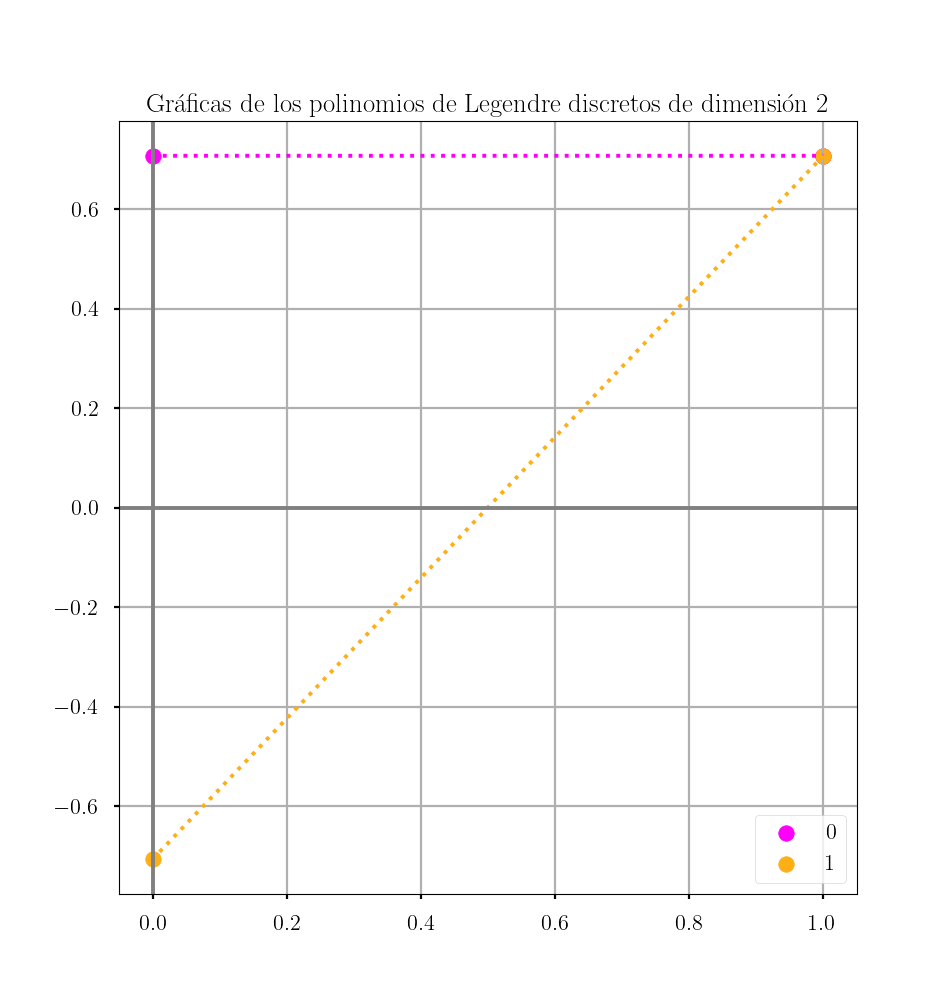
\includegraphics[scale =0.3 ]{PDL_dim2} 
 \end{figure}	 

\begin{figure}[H]
 	\sidecaption{
 	PDL de dimensión $3$.
 	\label{fig: PDL_dim3}
 	}
 	\centering
 	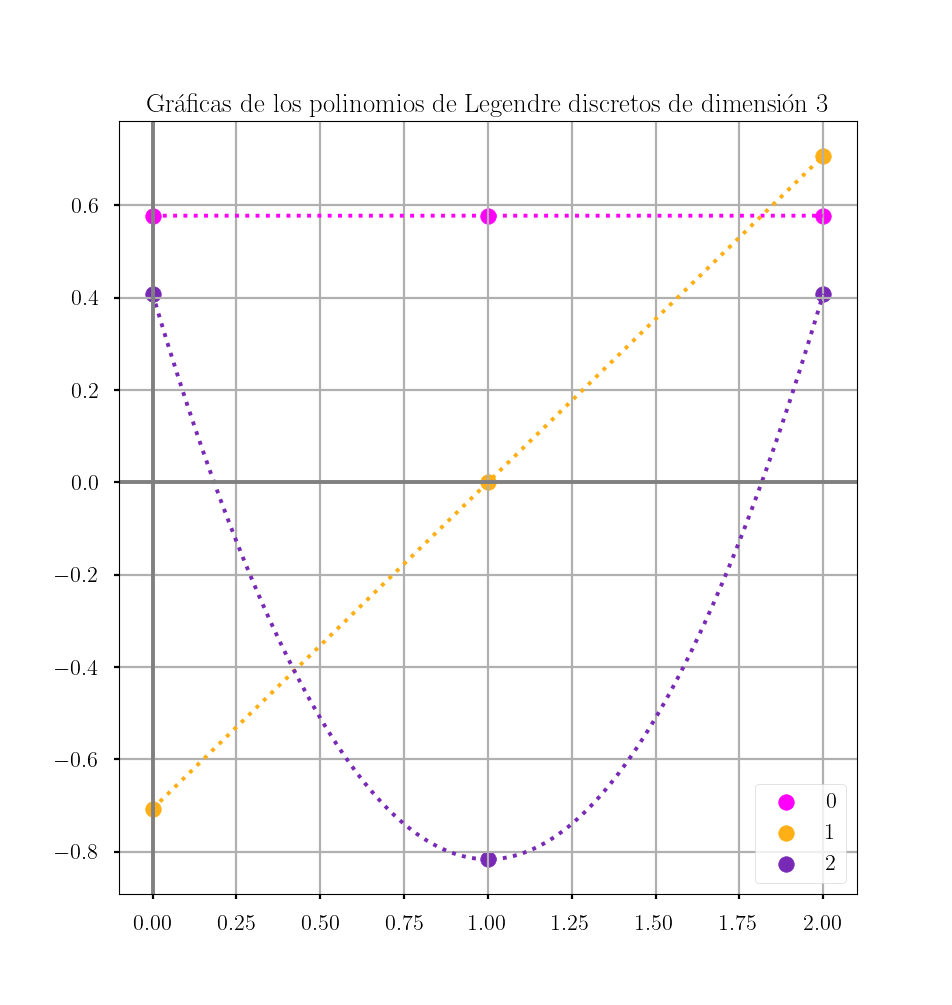
\includegraphics[scale =0.3 ]{PDL_dim3} 
 \end{figure}
 
 \begin{figure}[H]
 	\sidecaption{
 	PDL de dimensión $4$.
 	\label{fig: PDL_dim4}
 	}
 	\centering
 	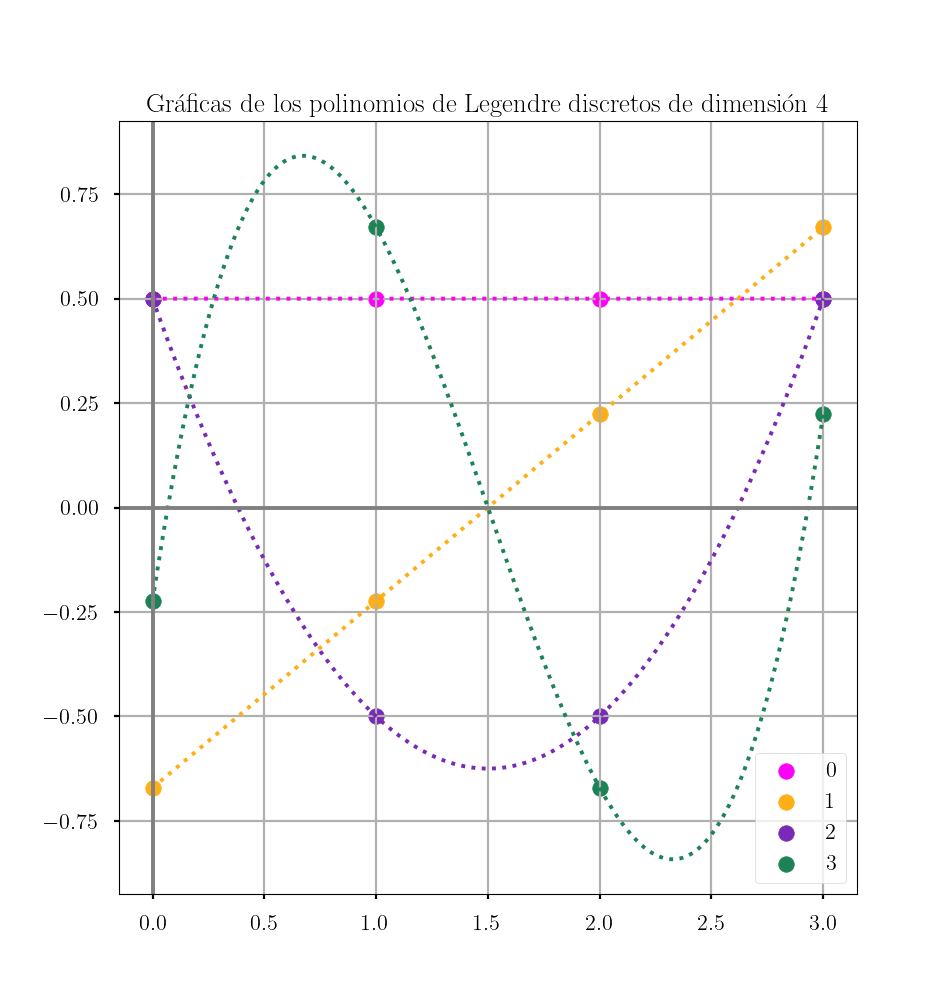
\includegraphics[scale =0.3 ]{PDL_dim4} 
 \end{figure}
 
  \begin{figure}[H]
 	\sidecaption{
 	PDL de dimensión $5$.
 	\label{fig: PDL_dim5}
 	}
 	\centering
 	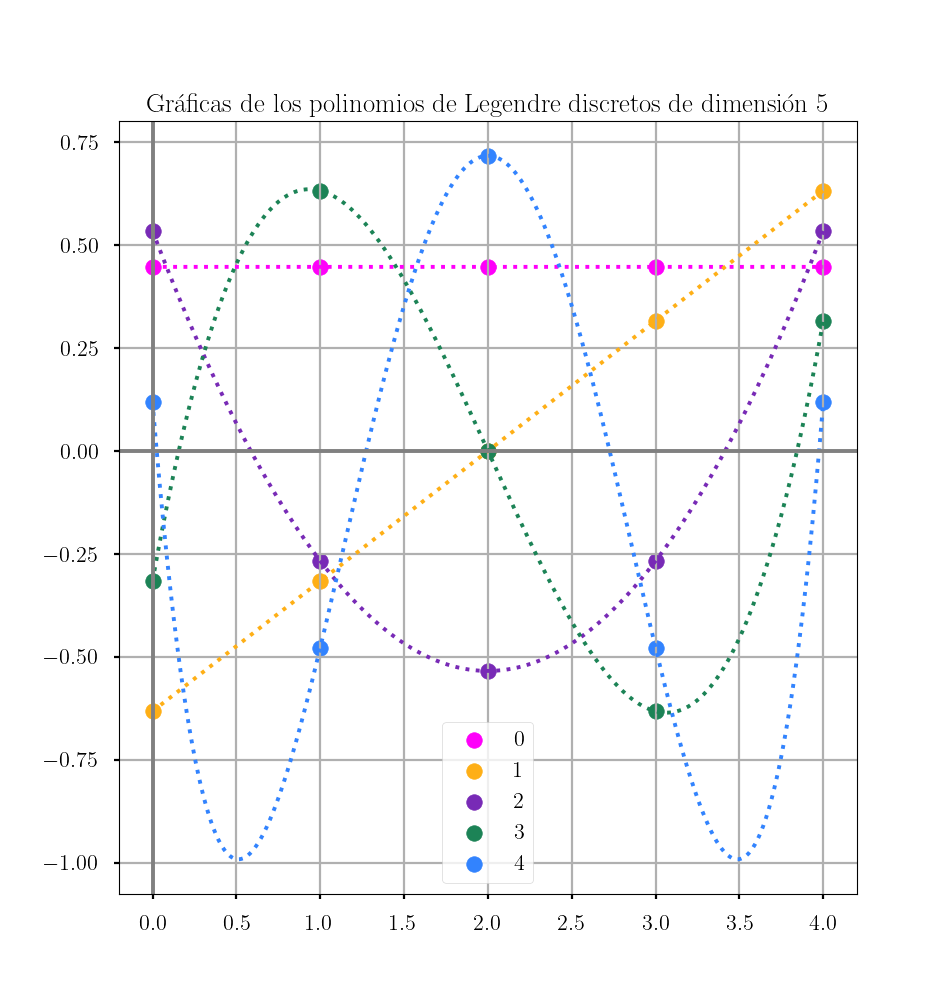
\includegraphics[scale =0.3 ]{PDL_dim5} 
 \end{figure}
 
   \begin{figure}[H]
 	\sidecaption{
 	PDL de dimensión $6$.
 	\label{fig: PDL_dim6}
 	}
 	\centering
 	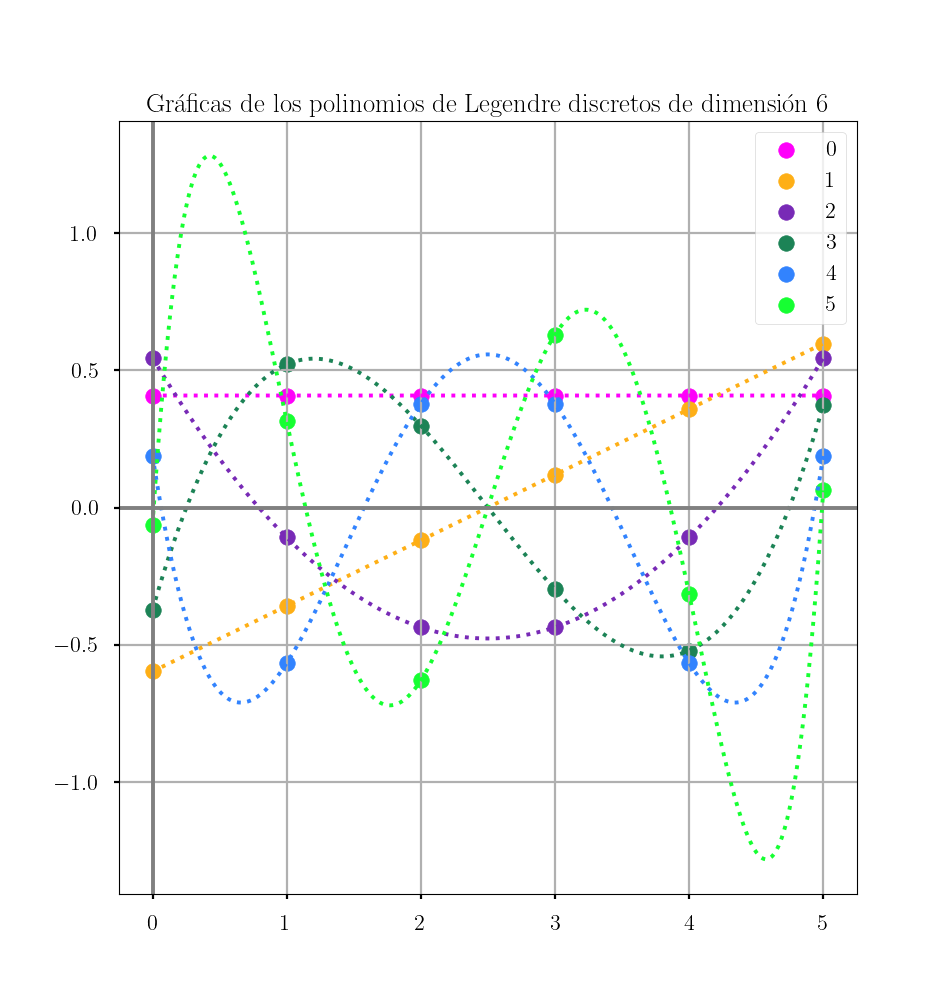
\includegraphics[scale =0.3 ]{PDL_dim6} 
 \end{figure}
 
   \begin{figure}[H]
 	\sidecaption{
 	PDL de dimensión $7$.
 	\label{fig: PDL_dim7}
 	}
 	\centering
 	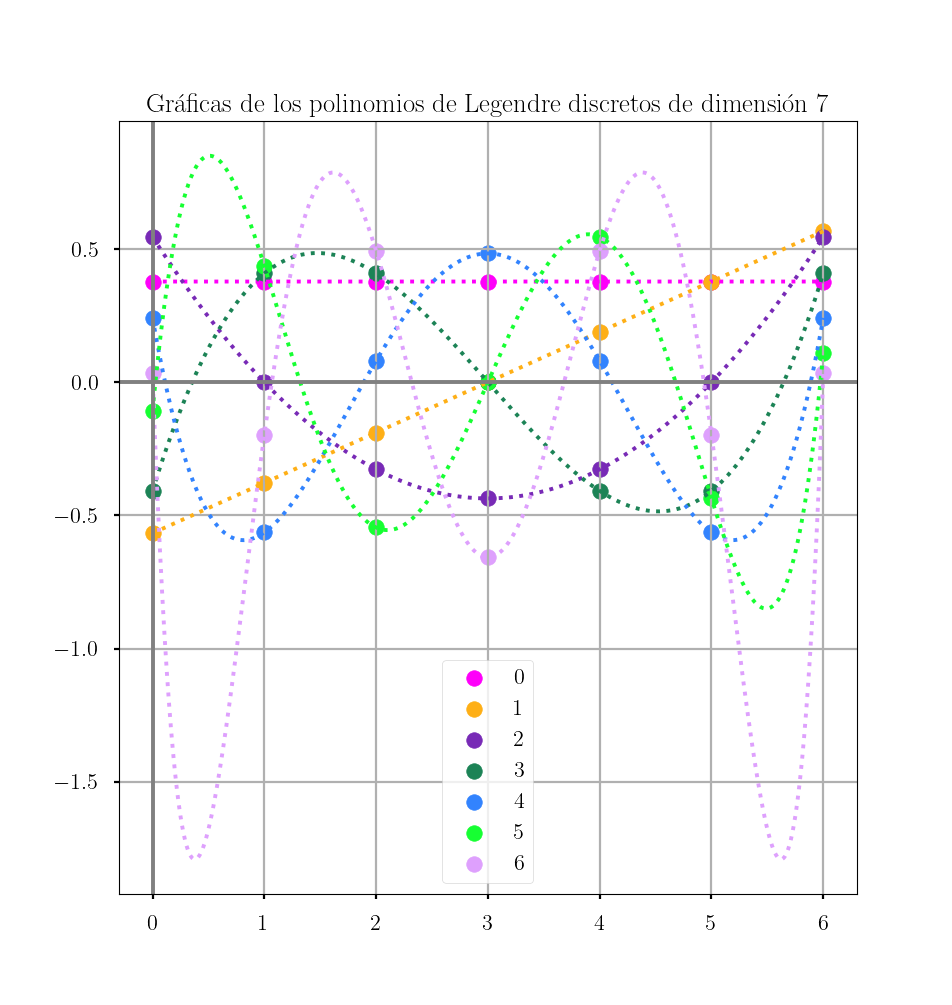
\includegraphics[scale =0.3 ]{PDL_dim7} 
 \end{figure}
 
   \begin{figure}[H]
 	\sidecaption{
 	PDL de dimensión $8$.
 	\label{fig: PDL_dim8}
 	}
 	\centering
 	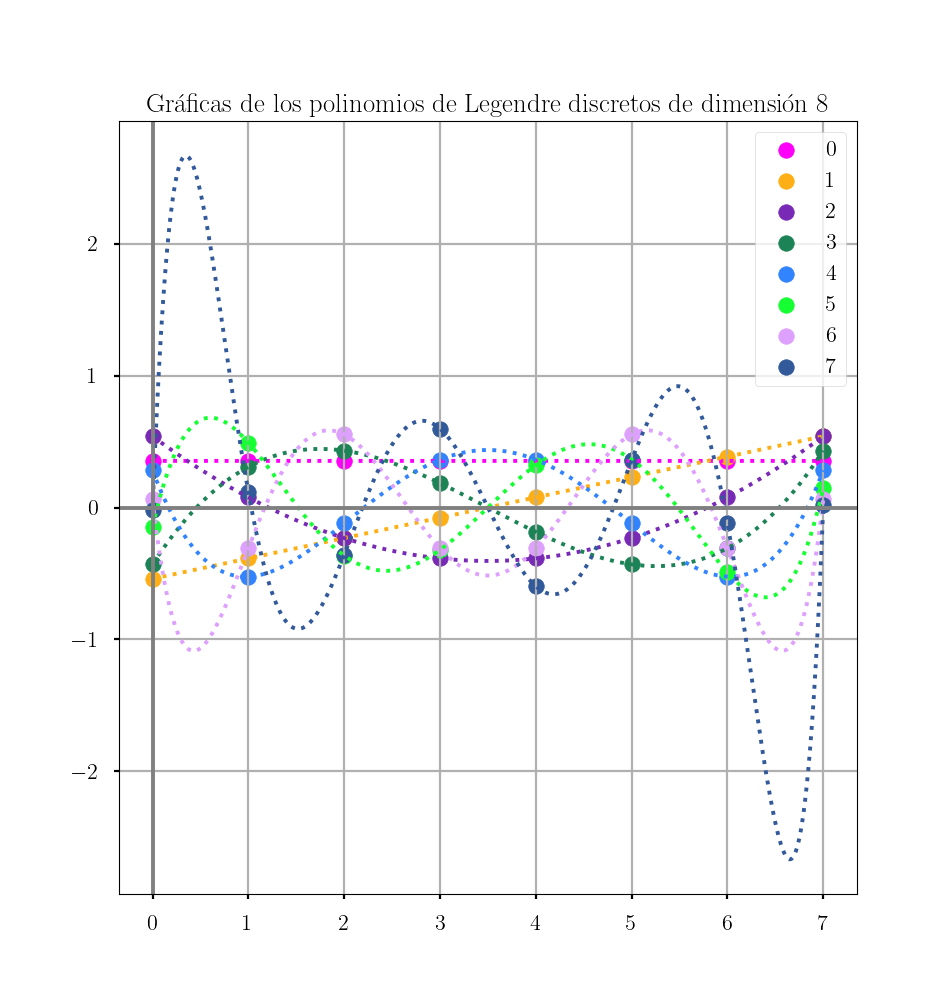
\includegraphics[scale =0.3 ]{PDL_dim8} 
 \end{figure}
%\section{Ejemplos}
\label{sec: ejemplos}
Definidas ya las bases de Legendre discretas
para toda dimensión $n$ 
(c.f. definición  
\ref{def: base de Legendre discreta}) y estudiadas algunas de sus 
propiedades, planteemos algunos ejemplos
para constatar en dimensiones concretas algunos de los
resultados demostrados en subsecciones anteriores
y empezar a comprobar la utilidad de estas bases para el 
estudio morfológico de señales finitas.


%Inicio ejemplo 1--------------------------------------------
\begin{ejemplo}
A continuación, mostramos las gráficas de los
elementos de las bases $\cali{L}^{2}$ y $\cali{L}^{3}$.
Para dibujar las gráficas usamos los valores
calculados en la tabla
\ref{formulas explicitas para Ln con n de 2 hasta 6}.

\begin{figure}[H]
	\sidecaption{
	Gráficas de los elementos de $\cali{L}^{2}
	\subseteq \IR^{2}$
	\label{fig: graficas elementos L2}
	}
	\centering
	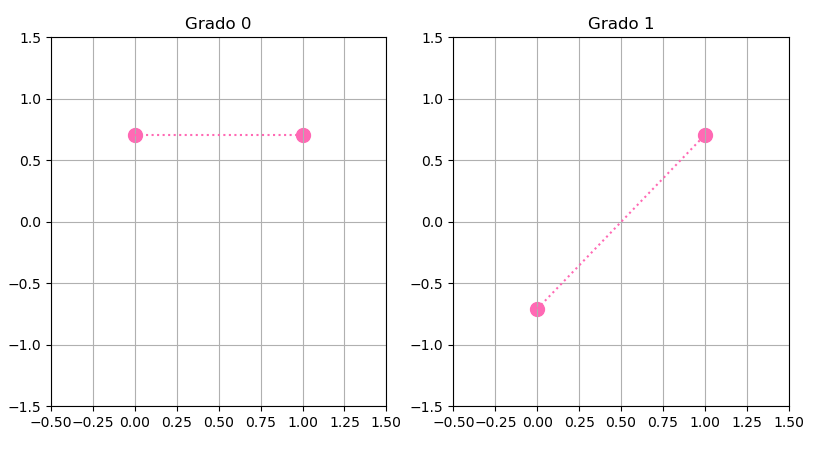
\includegraphics[scale=0.5]{graficasLegendre2} 
\end{figure}	


\begin{figure}[H]
	\sidecaption{
	Gráficas de los elementos de $\cali{L}^{3} 
	\subseteq \IR^{3}$
	\label{fig: graficas elementos L2}
	}
	\centering
	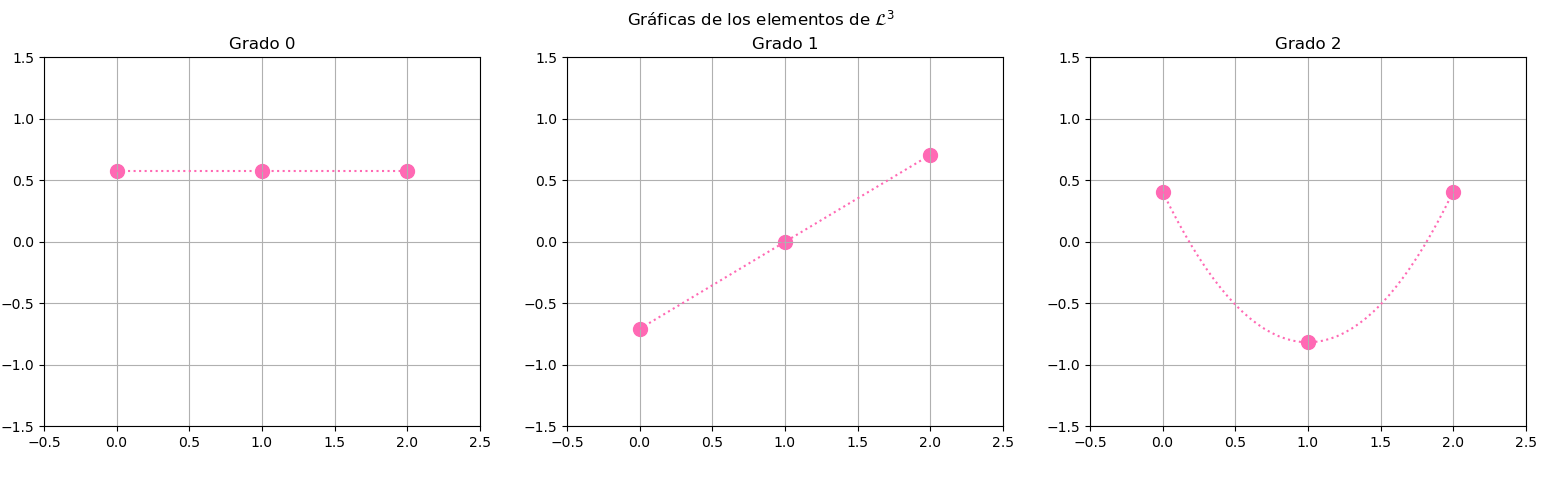
\includegraphics[scale=0.26]{graficasLegendre3} 
\end{figure}	




En el caso $n=2$, el único subespacio de polinomios
discretos no trivial es 
\begin{align*}
W_{2,0}= & span \left\{ 
\left(\frac{1}{\sqrt2}, \frac{1}{\sqrt2} \right) \right\} \\
= & \{ (x,x) \in \IR^{2}: \hspace{0.2cm} x \in \IR \},
\end{align*}

pues

\begin{equation}
\label{eq1: 1Dic}
W_{2,1}= \IR^{2}.
\end{equation}


En el caso $n=3$, calculamos que
\begin{align*}
W_{3,0}= & span \left\{
\left( \frac{1}{\sqrt3}, \frac{1}{\sqrt3},
\frac{1}{\sqrt3} \right) \right\}  \\
= & \{ (x,x,x) \in \IR^{3}: \hspace{0.2cm} x \in \IR \},
\end{align*}

\begin{align}
\label{eq2: 1Dic}
W_{3,1}= & span \left\{ \left( \frac{1}{\sqrt3}, \frac{1}{\sqrt3},
\frac{1}{\sqrt3} \right) ,
\left( -\frac{1}{\sqrt2}, 0,  \frac{1}{\sqrt2} \right) \right\}
\nonumber \\
= & \{ (x,y,2y-x) \in \IR^{3}: \hspace{0.2cm} x,y \in \IR \},
\end{align}
y
\[
W_{3,2}=\IR^{3}.
\]

\begin{figure}[H]
	\sidecaption{
	Gráficas de 
	$W_{2,0} \subseteq \IR^{2}$
	y de los subespacios
	$W_{3,0}$ y $W_{3,1}$ de $\IR^{3}$ que
	son, respectivamente, una recta y un plano;
	observe que
	$W_{3,0} \subseteq W_{3,1}$. 
	En ambas dimensiones se han 
	dibujado en {\color{ameMorado}{morado}} a los hiperplanos
	de polinomios discretos correspondientes, que en efecto
	dividen en dos regiones ajenas a los respectivos espacios 
	ambiente. La definición de hiperplano se da en
	\ref{section: hiperplanos}.
	\label{fig: graficas espacios W para dimensiones 2 y 3}
	}
	\centering
	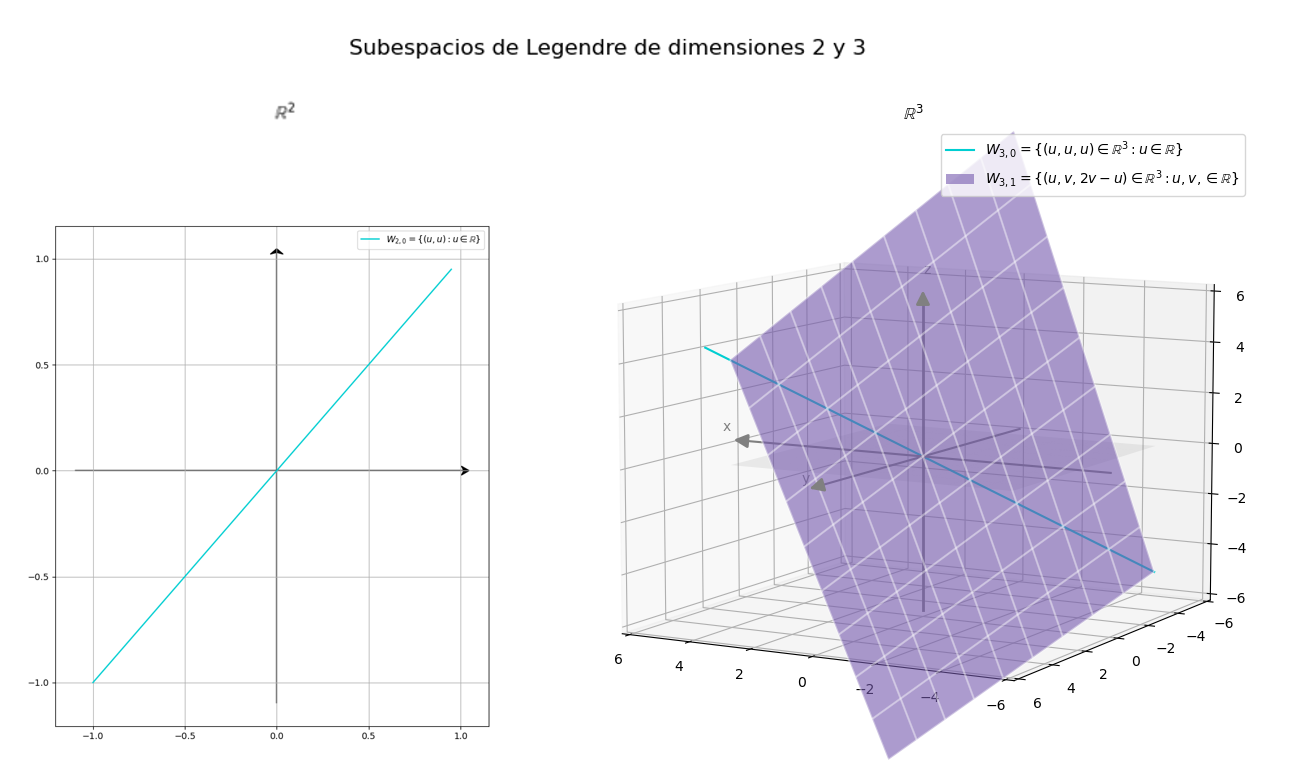
\includegraphics[scale= 1]{legendre2y3} 
\end{figure}	
	 
\final
\end{ejemplo}
%final ejemplo 1--------------------------------------------





%Inicio ejemplo 2--------------------------------------------

\begin{ejemplo}
Considere al siguiente conjunto de cinco
puntos del plano:
\begin{equation} \label{eq: conjunto cinco puntos}
\{ (0,-0.5), (1,2.4), (2, 1.6), (3,1.7), (4, 2.3) \}.
\end{equation}


Como tenemos cinco puntos, trabajamos
en el espacio $\IR^{5}$. 
La regresión lineal calculada a partir
del conjunto de datos
\eqref{eq: conjunto cinco puntos}
es la recta
con ecuación cartesiana

\begin{equation} \label{eq: recta minimos cuadrados}
y=0.49x+0.52.
\end{equation}

El vector cuyas entradas
son las cinco mediciones (dadas por las ordenadas
de los puntos del conjunto \eqref{eq: conjunto cinco puntos})
es
\begin{equation}
\label{eq0: 29Nov}
x=(-0.5, 2.4, 1.6, 1.7, 2.3).
\end{equation}


\begin{figure}[H]
	\sidecaption{
	Gráfica de la señal $x \in \IR^{5}$.
	\label{fig: grafica semal x ejemplo}
	}
	\centering
	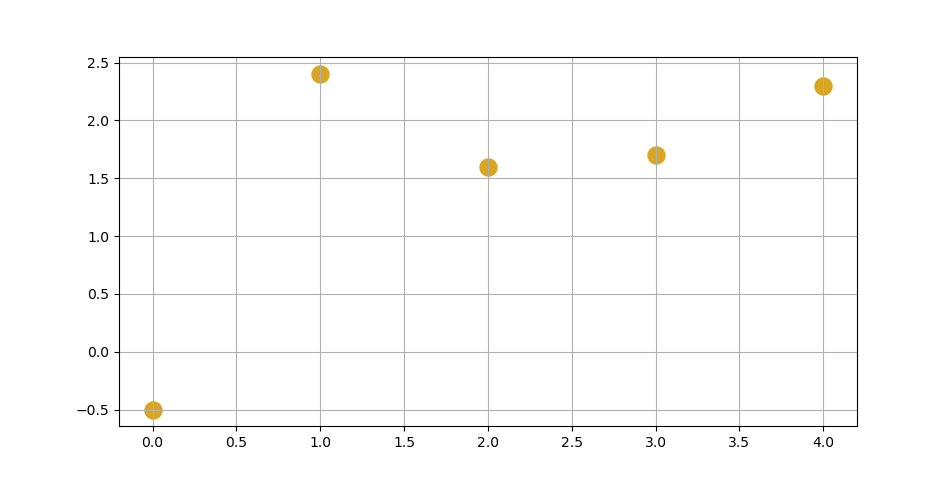
\includegraphics[scale=0.4]{graficaX_31Oct} 
\end{figure}	


Nos interesa
dar explícitamente a 
la señal $\Pi_{W_{5,1}}(x) \in W_{5,1} \leq \IR^{5}$.
En realidad, por ser $\cali{L}^{5}$ 
una base ortonormal de $\IR^{5}$ y por ser
$W_{5,1}$ el subespacio generado por los
dos primeros vectores de esta base, 
se sabe de inmediato que
\[
\Pi_{W_{5,1}}(x)=  \langle \Pi_{W_{5,1}}(x), \cali{L}^{5,0} \rangle \cali{L}^{5,0}
+ \langle \Pi_{W_{5,1}}(x), \cali{L}^{5,1} \rangle \cali{L}^{5,1};
\]
de todas formas, como ilustración, planteemos un sistema
de ecuaciones para llegar a una expresión para
$\Pi_{W_{5,1}}(x)$.
Usando las expresiones para los vectores
de $\cali{L}^{5}$
dadas en \ref{subsect:Formulas explicitas},
tenemos que
\[
W_{5,1}=span\{ (1,1,1,1,1,1), (-2, -1, 0, 1, 2) \},
\]

y 
\[
W_{5,1}^{\perp}=span\{ (2,-1,-2,-1,2), (-1,2,0,-2,1), (1,-4,6,-4,1)\}.
\]
Según el teorema de la proyección ortogonal \ref{Teo:proyOrt},
$\Pi_{W_{5,1}}(x)$ es el único elemento de $W_{5,1}$ para el 
que 

\[
x-\Pi_{W_{5,1}}(x) \in W_{5,1}^{\perp};
\]
esto se 
traduce en la existencia de 
únicos escalares $c_{1}$, $c_{2}$,
$a_{1}$, $a_{2}$ y $a_{3}$ tales que
\[
x-c_{1}(1,1,1,1,1)-c_{2}(-2, -1, 0, 1, 2)
\]
es igual a 

\[
a_{1}(2,-1,-2,-1,2)+a_{2}(-1,2,0,-2,1)
+ a_{3}(1,-4,6,-4,1),
\]
\noindent
o sea, tales que

\begin{equation*}
\begin{cases}
-0.5-(c_{1}-2c_{2})=2a_{1}-a_{2}+a_{3}, \\
2.4-(c_{1}-c_{2})=-a_{1}+2a_{2}-4a_{3}, \\
1.6-c_{1}=-2a_{1}+6a_{3},\\
1.7-(c_{1}+c_{2})=-a_{1}-2a_{2}-4a_{3}, \\
2.3-(c_{1}+2c_{2})=2a_{1}+a_{2}+a_{3}.
\end{cases}
\end{equation*}
Resolviendo este sistema
de ecuaciones, encontramos que
$c_{1}=1.5$ y $c_{2}=0.49$. Así,




\begin{align}
\label{eq5: 23Oct}
\Pi_{W_{5,1}}(x) =& c_{1} (1,1,1,1,1) + c_{2}(-2-1,0,1,2) \nonumber \\
= & (0.52, 1.01, 1.5, 1.99, 2.48 );
\end{align}
observe que \eqref{eq5: 23Oct} es, 
en efecto, la discretización de 
la recta \eqref{eq: recta minimos cuadrados}
en la malla uniforme $\cali{P}_{5}$.
De forma análoga se calcula la parte cuadrática de
la señal $s$.

\begin{figure}[H]
	\sidecaption{
	Gráficas de $x$, 
	$\Pi_{W_{5,0}}(x)$, $\Pi_{W_{5,1}}(x)$ y $\Pi_{W_{5,2}}(x)$.
	\label{fig: partes afin, lineal y cuadratica} 
	}
	\centering
	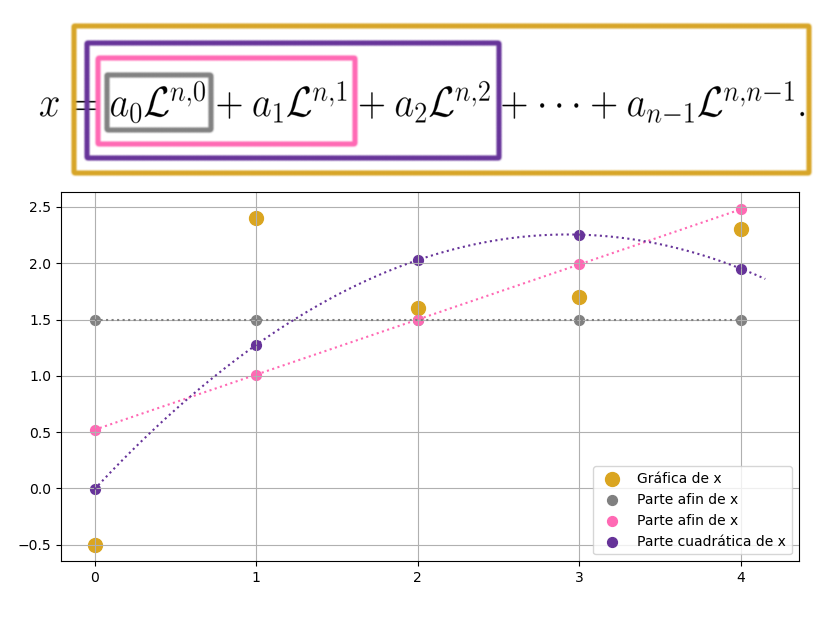
\includegraphics[scale=0.6]{parteAfinCuadr}
\end{figure}	
\final
\end{ejemplo}
%Final ejemplo 2--------------------------------------------


\TODO{Sería bueno notar que estas dando un
algoritmo de transformación de la raw data
via una proyección lineal (proceso mediante
en cual se destruye información). Nada de ML, 
esto es más bien symbolic AI (deep learning with
python, p.35)}



En el siguiente ejemplo 
damos dos propuestas naturales,
usando los espacios de polinomios discretos $W_{n,k}$,
para poder dar no sólo respuestas del tipo
``sí/no'' a preguntas sobre la morfología de una señal, sino,
de forma más general, del tipo ``qué tanto sí'' o
``qué tanto no''.



%Inicio ejemplo 3--------------------------------------------

\begin{ejemplo}
Hagamos $n=3$.  
Como se calculó en \eqref{eq2: 1Dic},
el subespacio $W_{3,1} \leq \IR^{3}$ de señales afines es el plano
de ecuación cartesiana

\[
W_{3,1}: \hspace{0.2cm} x-2y+z=0.
\]
Sea 
\begin{equation*}
\label{eq0: 9Feb}
x=a_{0}\cali{L}^{3,0}+a_{1}\cali{L}^{3,1}+a_{2}\cali{L}^{3,2}
\end{equation*}
un vector del espacio.
Como se argumentó ya, las proposiciones
\begin{center}
``$x \in \IR^{3}$ es afín'' \hspace{0.2cm} y \hspace{0.2cm} 
``$x \in W_{3,1}$''
\end{center} 
son equivalentes.
Observe que es ``poco probable'' que, al seleccionar al azar
un vector de $\IR^{3}$, este sea afín (pues el 
subconjunto $W_{3,1}$ de $\IR^{3}$,
un plano, tiene
medida de Lebesgue cero); sin embargo, provistos
de nociones como las de norma y ortogonalidad, es fácil dar 
propuestas legítimas de
\textbf{medidas} de ``qué tan afín'' es la señal $x$,
o, en términos matemáticos, de qué tanto se aleja
$x$ del espacio de señales afines de su correspondiente
espacio ambiente.

\begin{figure}[H]
	\sidecaption{
	Esquema de dos formas en las que uno puede intentar medir
	qué tan afín es una señal $x$.
	\label{fig: dos formas de medir distancia a plano}
	}
	\centering
	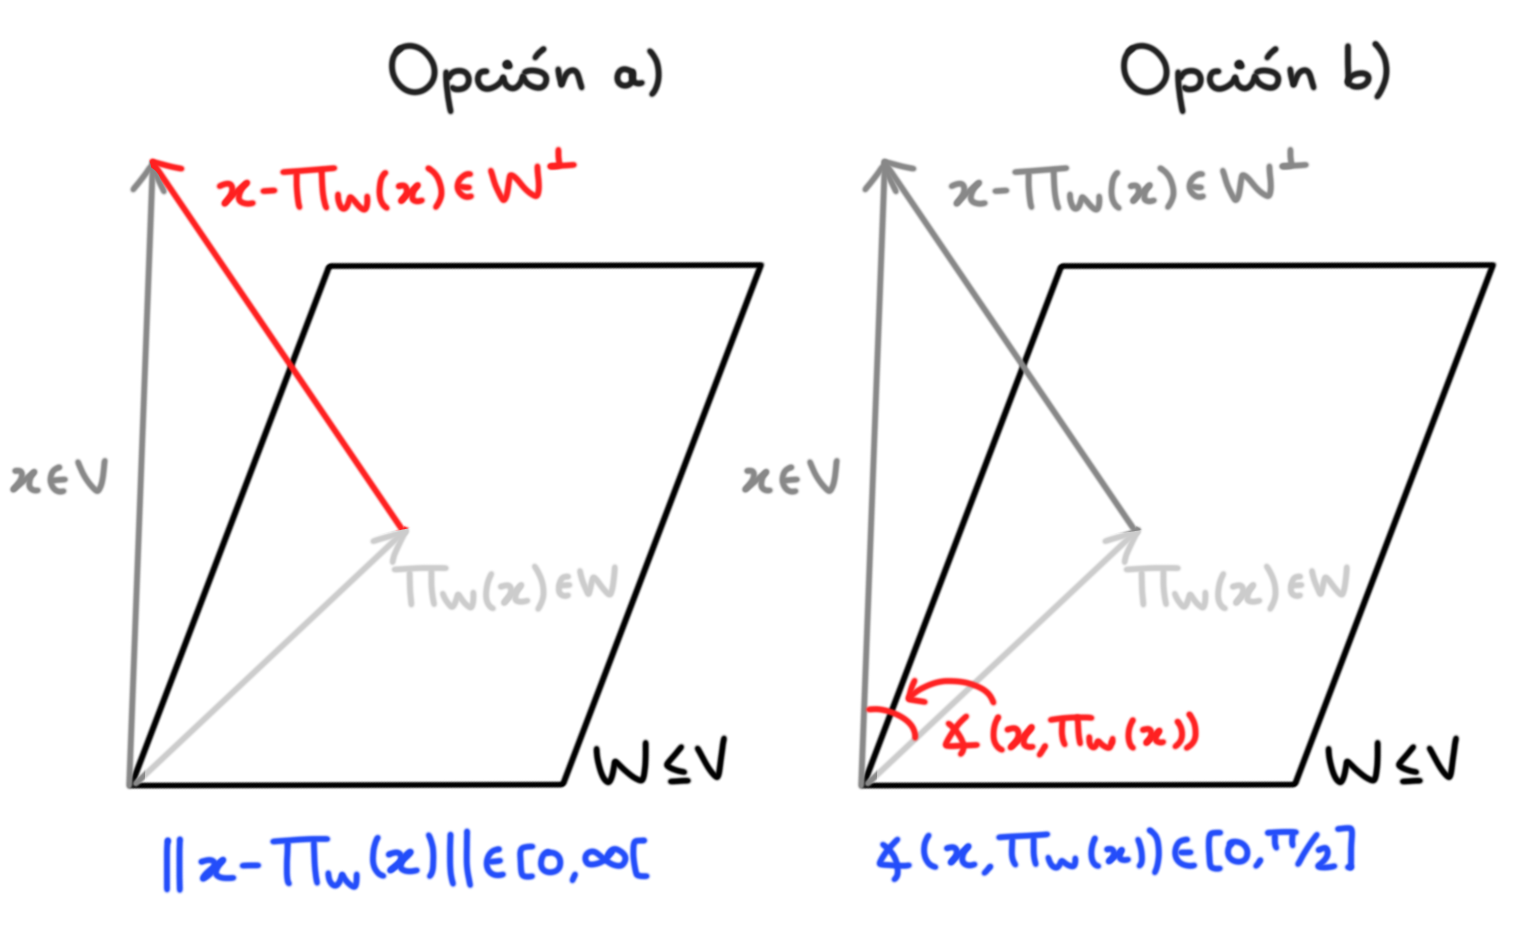
\includegraphics[scale= 1]{ 18Sept_1} 
\end{figure}	

\TODO{
Recuerda que debes de notar que la distancia al plano en realidad
no es la mejor forma de dar una medida de qué tan afín
es $x$.}

\begin{itemize}
\item[a)] Una forma obvia de proceder es calcular la norma
del vector 
\[
x - \Pi_{W_{3,1}}(x)= a_{2} \cali{L}^{3,2},
\]
es decir, tomar al número no negativo
\[
|a_{2}|
\]
como una medida de qué tanto se aleja $x$ del plano $W_{3,1}$
(o sea, de qué tanto se aleja $x$ de ser afín.)

\item[b)] Otro acercamiento podría ser preguntarse por
el ángulo $\alpha \in [0, \frac{\pi}{2}]$ 
que forma el vector $x$ con el espacio 
$W_{3,1}$. Los casos extremos $\alpha=0$ y $\alpha= \frac{\pi}{2}$
corresponden, respectivamente, a que $x$ sea afín y
a que $x$ sea múltiplo escalar de $\cali{L}^{3,2}$, luego,
a que sea ortogonal a cualquier señal afín de dimensión 3.

Como las dimensiones de $\IR^{3}$ y $W_{3,1}$ 
difieren por uno,
este útimo es un hiperplano
\sidenote{Puede recordar la definición
de hiperplano en 
\ref{section: hiperplanos}.}
del primero; como $\cali{L}^{3,2}$
es un vector normal a $W_{3,1}$
(c.f. corolario \ref{cor: Ln,k ortogonal a todo pol discreto de grado menor a k}), 
si $\varphi: \IR^{3} \longrightarrow \IR$ es la función
definida como
\begin{equation}
\label{eq: funcion phi ejemplo}
\varphi(x)= \langle \cali{L}^{3,2} , x \rangle =a_{2},
\end{equation}



las tres regiones ajenas en las
que $W_{3,1}$ divide al espacio
$\IR^{3}$ son 


\begin{itemize}
\item[I)] $\{ x \in \IR^{3} : \varphi(x)>0 \}$,
región a la que pertenece $\cali{L}^{3,2}$,
\item[II)] $W_{3,1}= Ker(\varphi)$, y 
\item[III)] $\{ x \in \IR^{3} : \varphi(x)<0 \}$,
región a la que pertenece $-\cali{L}^{3,2}$.
\end{itemize}



\begin{figure}[H]
\centering\captionsetup{format = hang}
	\begin{measuredfigure}
		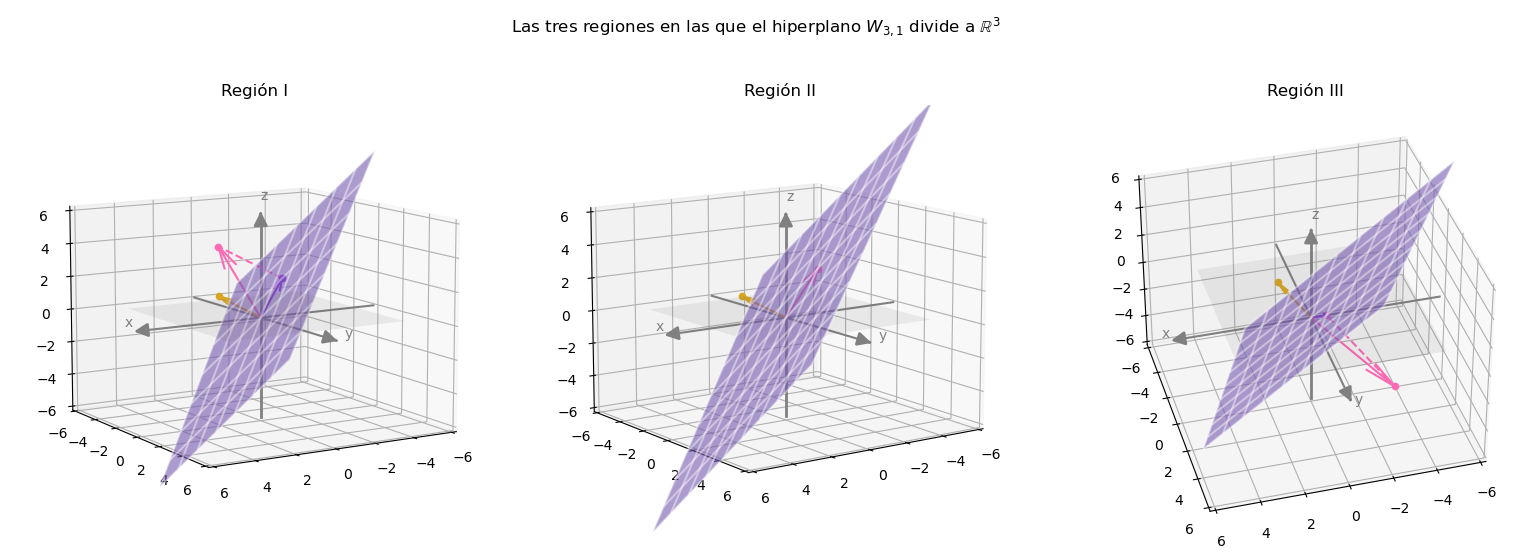
\includegraphics[scale=0.85]{2Dic_4} 
		\caption{Se ilustran las tres 
		regiones en las que $W_{3,1} \subseteq \IR^{3}$ divide al espacio,
		clasificadas según el signo que tome 
		la función $\varphi$ como se definió en
		\eqref{eq: funcion phi ejemplo}. En
		{\color{ameDorado}{dorado}} se muestra al vector
		$\cali{L}^{3,2}$, en {\color{ameRosa}{rosa}}
		un elemento de la región citada, y en 
		{\color{ameMorado}{morado}} la proyección de este
		al espacio $W_{3,1}$.
		}
 	\end{measuredfigure}
 \end{figure}

Es fácil obtener una expresión para el coseno del ángulo
$\alpha$ en términos de los coeficientes de $x$ respecto a $\cali{L}^{3}$:

\begin{figure}[H]
\centering\captionsetup{format = hang}
	\begin{measuredfigure}
		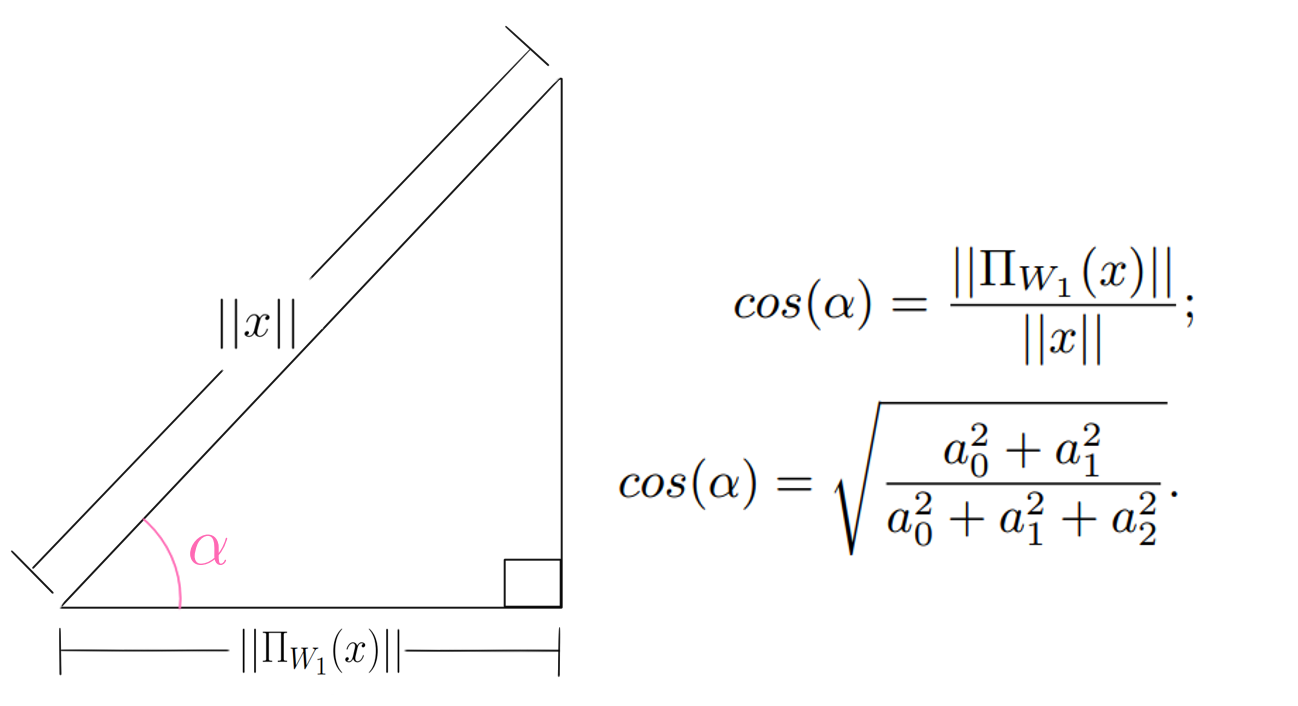
\includegraphics[scale=0.7]{2Dic_3} 
		\caption{\TODO{por qué ese ángulo era recto?}}
 	\end{measuredfigure}
 \end{figure}

De las relaciones de la figura \TODO{ref}
obtenemos una igualdad que relaciona el ángulo 
$\alpha$ que forma una señal $x \in \IR^{3}$ 
con su proyección al espacio $W_{3,1}$
con los coeficientes $a_{i}$
de $x$ respecto a $\cali{L}^{3}$:
\begin{equation}
\label{eq0: 3Dic}
cos(\alpha)= \sqrt{\frac{a_{0}^{2}+a_{1}^{2}}{a_{0}^{2}+a_{1}^{2}+a_{2}^{2}}}.
\end{equation}

Para un ejemplo aún más concreto, hagamos 
\begin{equation}
\label{eq1: 19Sept}
a_{0}= \sqrt{3}, \hspace{0.2cm} a_{1}= \sqrt{2},
\end{equation}



es decir, consideremos a todos los vectores de $\IR^{3}$
cuya proyección al plano $W_{3,1}$ es 
el vector
\begin{equation}
\label{eq1: 6Dic}
(0,1,2).
\end{equation}
Es obvio que el conjunto de los puntos
del espacio cuyas proyecciones a 
$W_{3,1}$ es \eqref{eq1: 6Dic} de hecho es la recta
con ecuación vectorial
\begin{equation}
\label{eq0: 6Dic}
l_{(0,1,2)} := (0,1,2)+c(1,-2,1), \hspace{0.2cm} c \in \IR.
\end{equation}

Sustituyendo
los valores \eqref{eq1: 19Sept} en \eqref{eq0: 3Dic} y
despejando, obtenemos 
\[
|a_{2}|= \sqrt{5 tg^{2}(\alpha)};
\]
el signo del coeficiente $a_{2}$ (que corresponde a la dirección
de $\cali{L}^{3,2}$ en la descomposición de $x$) se determina por
la región en la que se encuentre $x$;

\begin{itemize}
\item el signo de $a_{2}$ es positivo si $x$ es elemento de la región I,
\item $a_{2}=0$ si $x$ es elemento de la región II, y
\item el signo de $a_{2}$ es negativo si $x$ es elemento de la región III.
\end{itemize}


Grafiquemos ahora algunos elementos
de la recta \eqref{eq0: 6Dic}; en los pies
de la figura se especifica el ángulo
$\alpha$ que forma con su proyección así
como la región del espacio a la que pertenece.
Los valores de las entradas de $x$, en la
mayoría de los casos, han sido redondeados.
\end{itemize}
\begin{figure}[H]
\centering\captionsetup{format = hang}
	\begin{measuredfigure}
		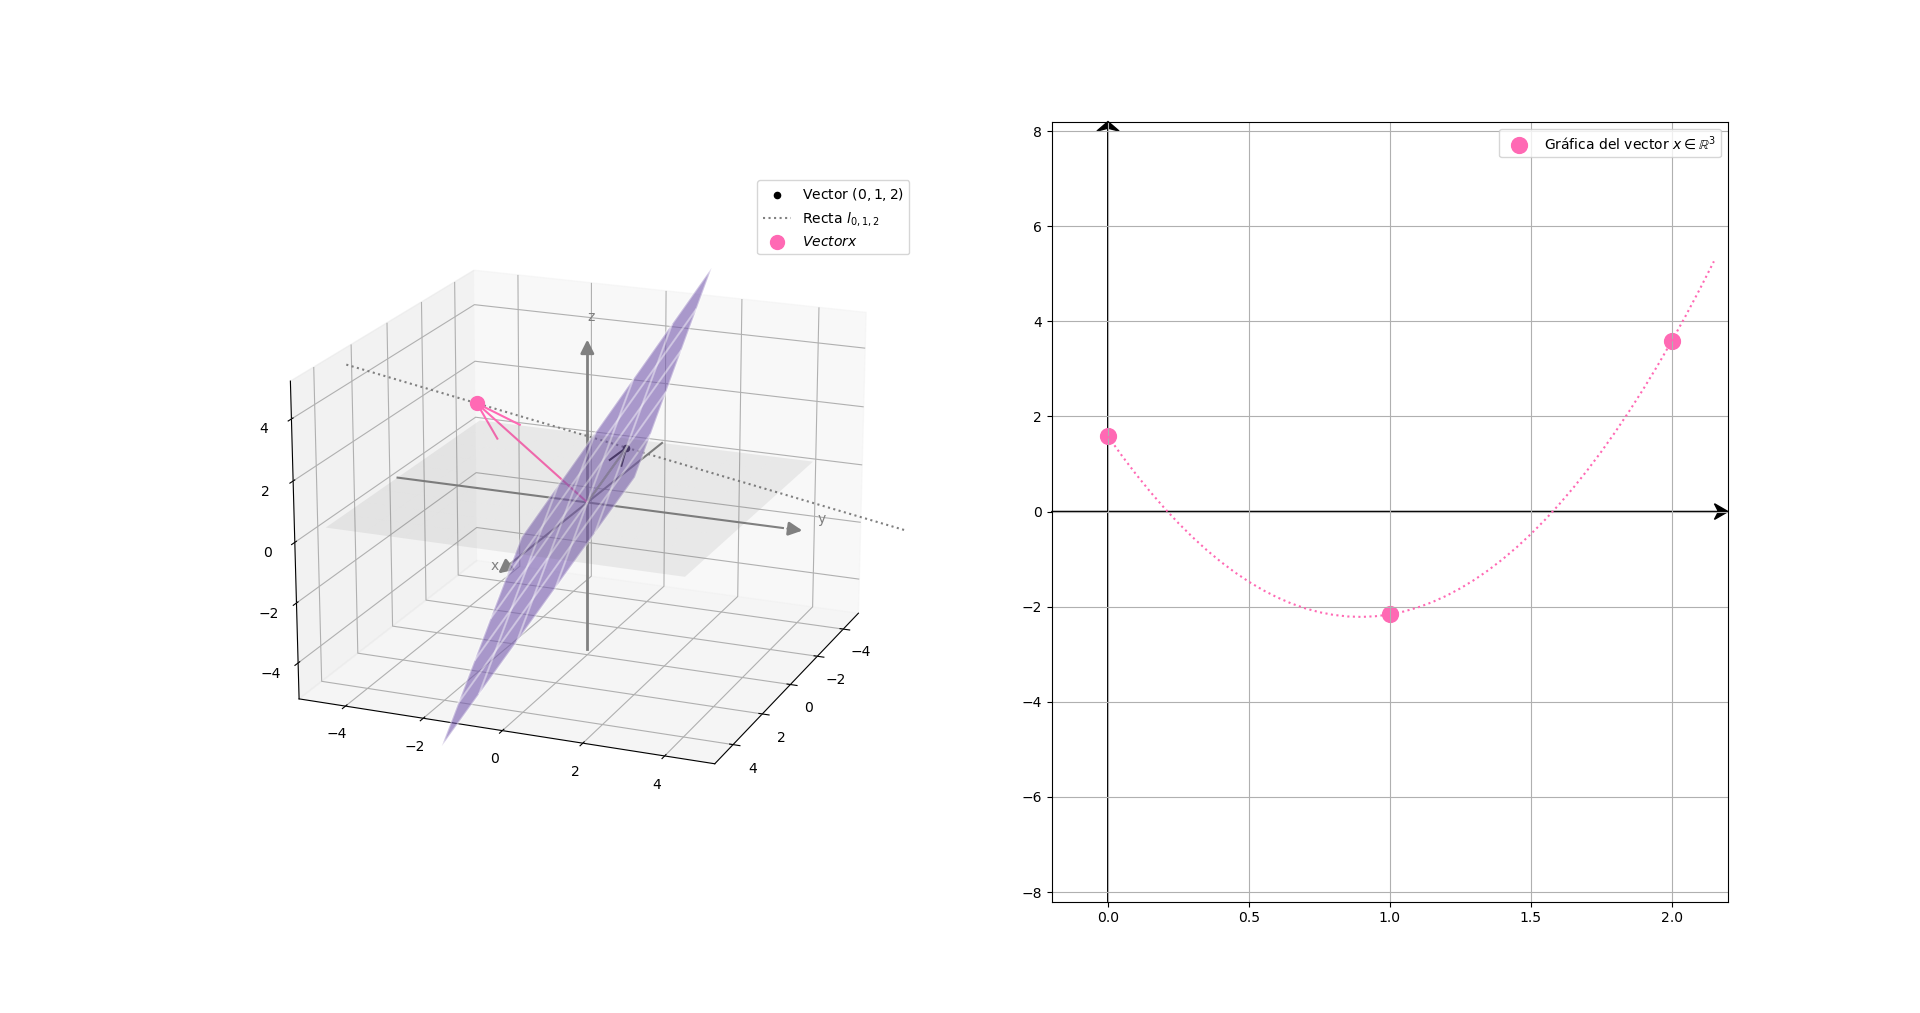
\includegraphics[scale=0.33]{6Dic_0} 
		\caption{Aquí se considera al vector 
		$x=(1.58, -2.16,3.58)$ que forma un ángulo $\alpha=\pi/3$
		con el plano $W_{3,1}$ y que se ubica en la región I.
		\TODO{te faltó graficar al vector normal L3,2.}}
 	\end{measuredfigure}
 \end{figure}


\begin{figure}[H]
\centering\captionsetup{format = hang}
	\begin{measuredfigure}
		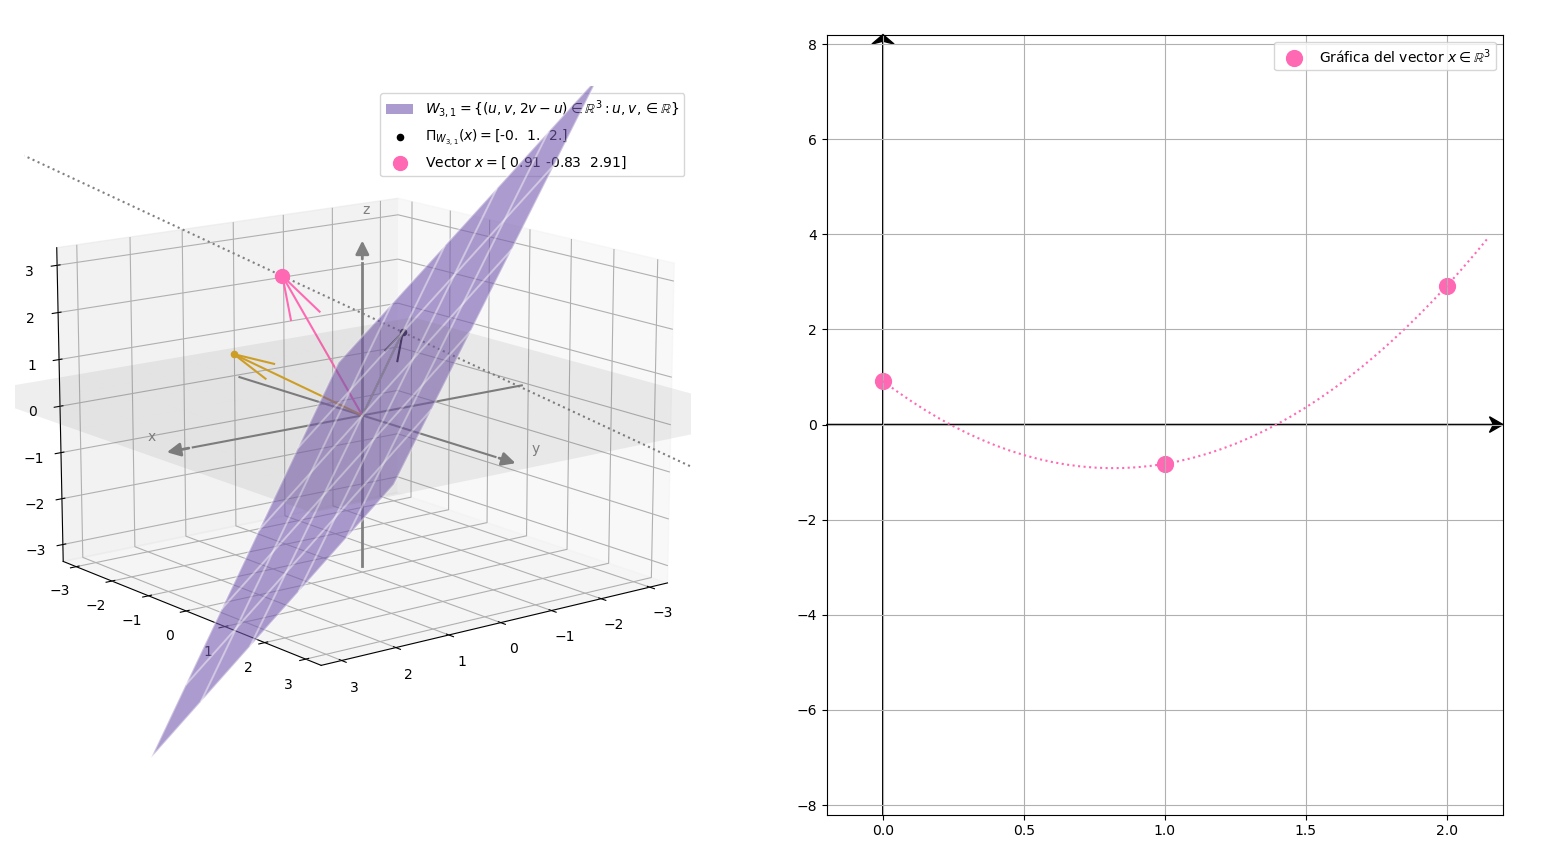
\includegraphics[scale=0.33]{6Dic_1} 
		\caption{Aquí se considera al vector 
		$x=(0.91,-0.82,2.91)$ que forma un ángulo $\alpha=\pi/4$
		con el plano $W_{3,1}$ y que se ubica en la región I.}
 	\end{measuredfigure}
 \end{figure}
 
 
\begin{figure}[H]
\centering\captionsetup{format = hang}
	\begin{measuredfigure}
		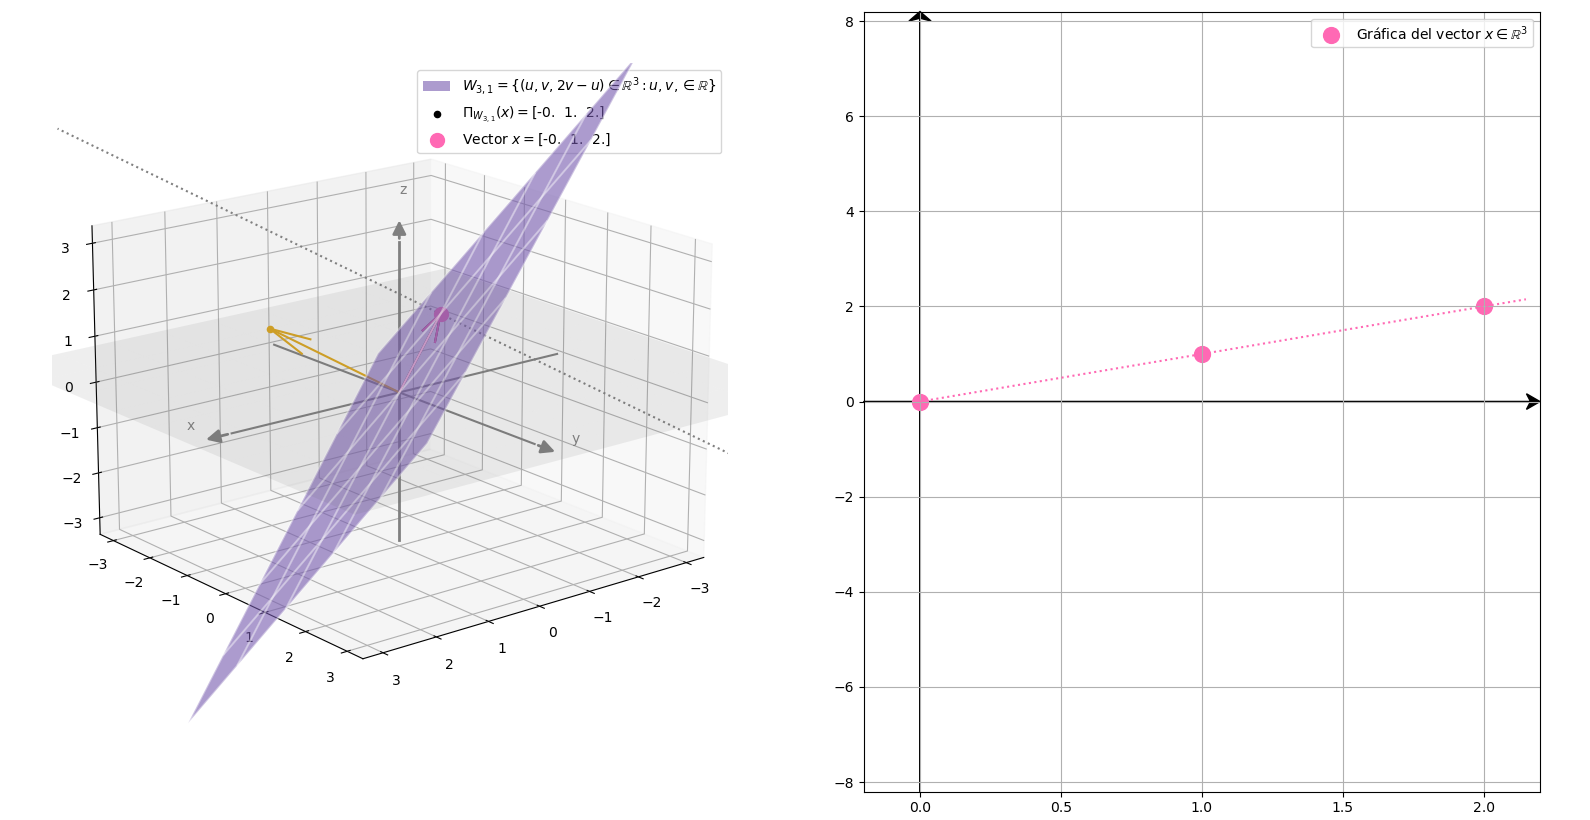
\includegraphics[scale=0.33]{6Dic_2} 
		\caption{Aquí se considera al vector 
		$x=(0,1,2)$ que forma un ángulo $\alpha=0$
		con el plano $W_{3,1}$ y que se ubica en la región II.}
 	\end{measuredfigure}
 \end{figure}

\begin{figure}[H]
\centering\captionsetup{format = hang}
	\begin{measuredfigure}
		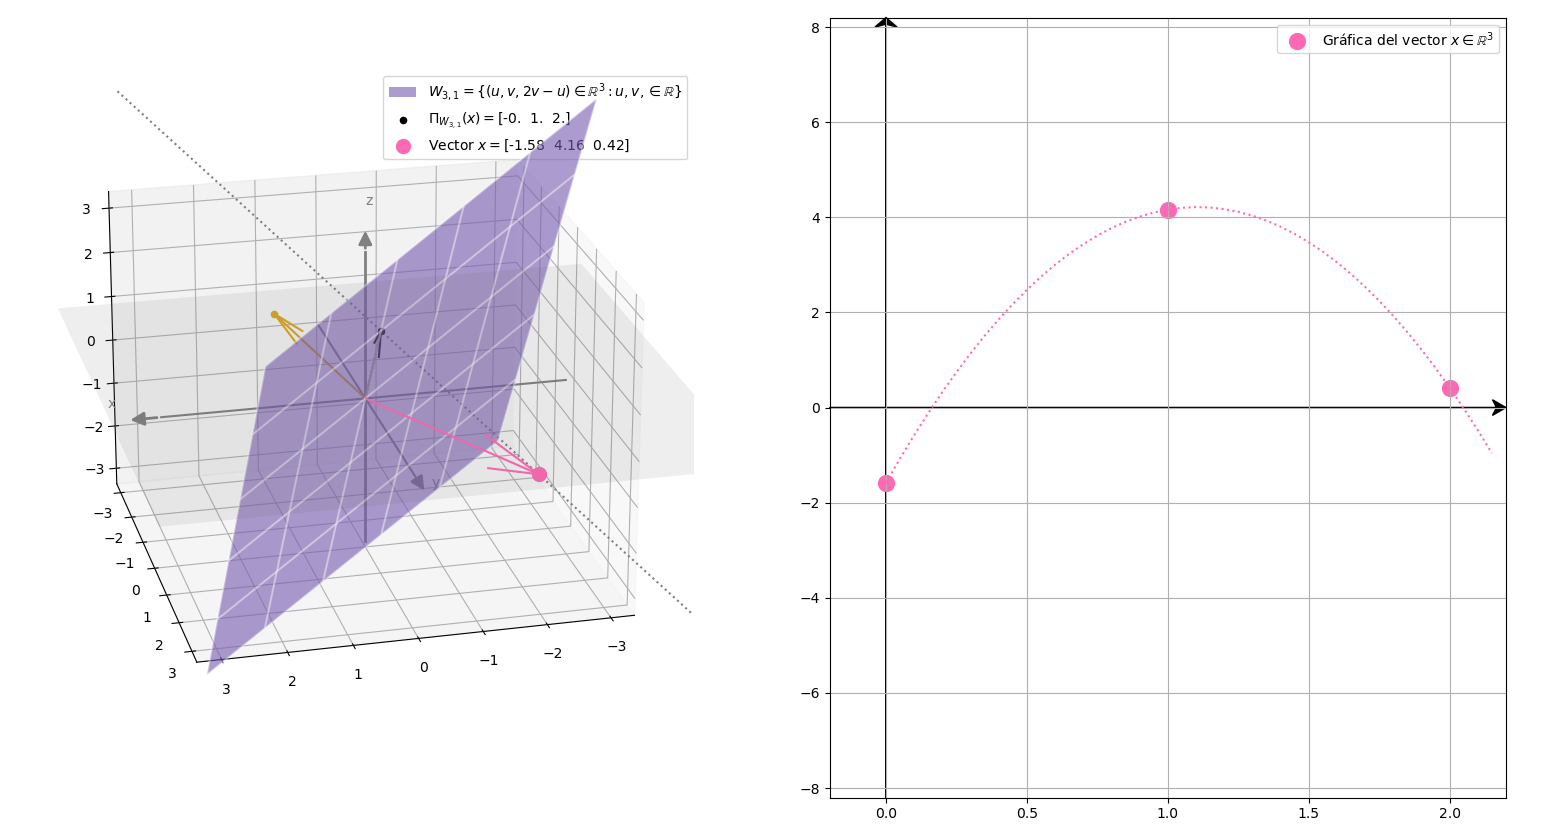
\includegraphics[scale=0.33]{6Dic_3} 
		\caption{Aquí se considera al vector
		$x=(-1.58,4.16,0.41)$ que forma un ángulo $\alpha=\pi/3$
		con el plano $W_{3,1}$ y que se ubica en la región III.}
 	\end{measuredfigure}
 \end{figure}
 
 
\begin{figure}[H]
\centering\captionsetup{format = hang}
	\begin{measuredfigure}
		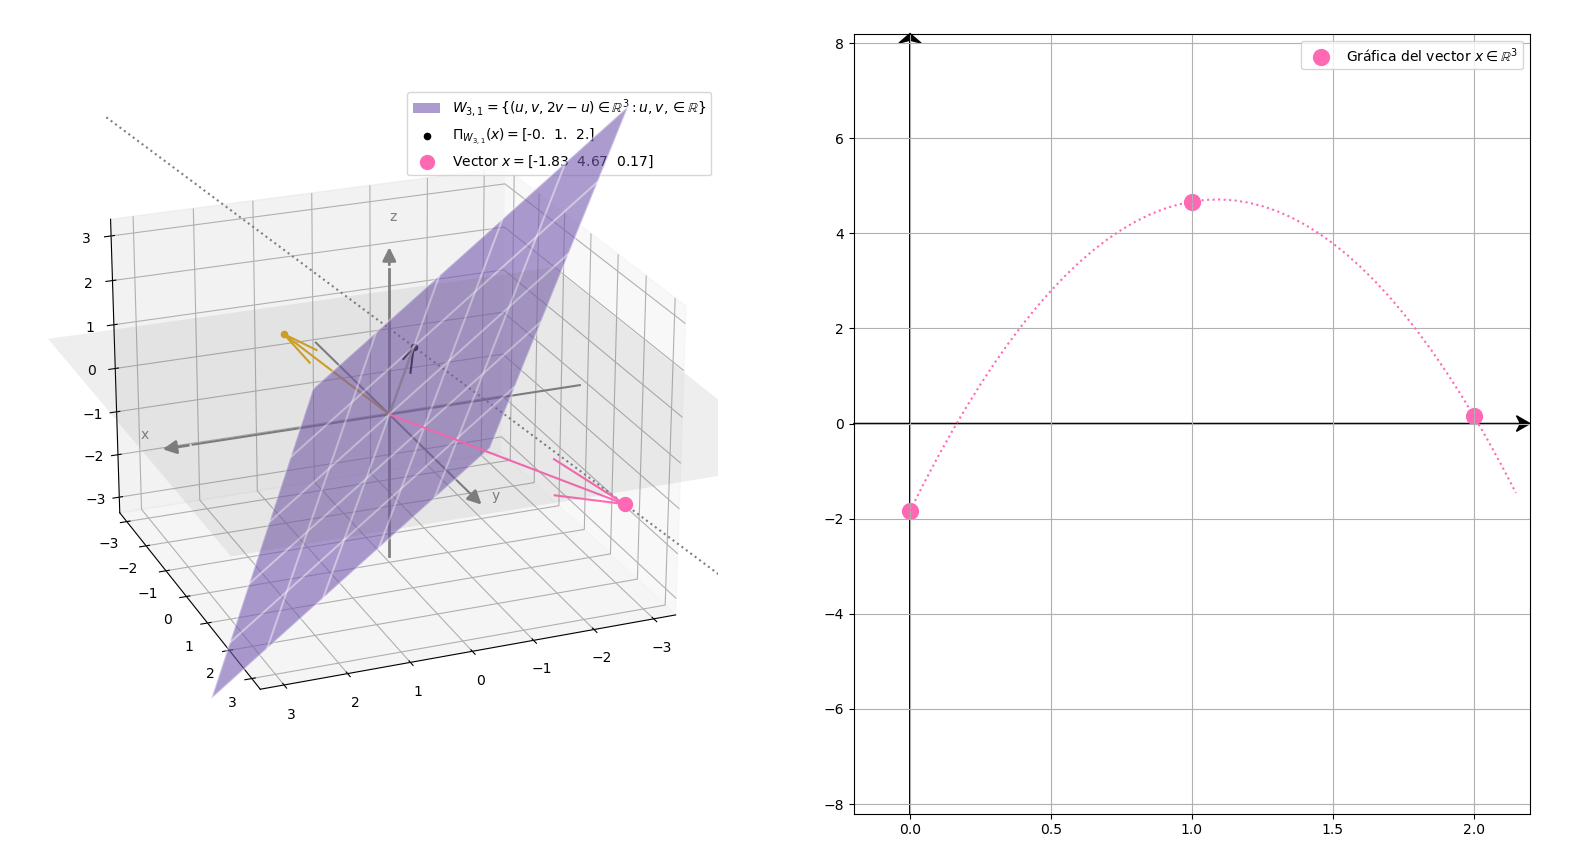
\includegraphics[scale=0.33]{6Dic_4} 
		\caption{Aquí se considera al vector 
		$x=(-1.83,4.66,0.16)$ que forma un ángulo $\alpha=6\pi/17$
		con el plano $W_{3,1}$ y que se ubica en la región III.}
 	\end{measuredfigure}
 \end{figure}
 
 

Veamos por qué, en realidad, la alternativa $b)$
descrita arriba es mucho mejor que la $a)$ para cuantificar 
la morfología de una señal finita.

Si $x \in \IR^{n}$ es una señal de dimensión $n$ y 
$\lambda \in \IR-\{ 0 \}$ es un escalar cualquiera,
la gráfica de $\lambda x$ no es más que la gráfica 
de $x$ reescalada por un factor de $\lambda$ cuando este
último es positivo; en caso contrario, es la gráfica
de $x$ reescalada pero además reflejada respecto al eje
horizontal.


\final
\end{ejemplo}
%Final ejemplo 3--------------------------------------------
 
%\chapter{Sobre simetrías en las entradas de los polinomios de Legendre discretos}
\label{section: sobre simetrias en las entradas de los poliomios discretos de Legendre}
Puesto que planeamos implementar computacionalmente
las bases de Legendre discretas, es de utilidad 
buscar simetrías en las entradas de los vectores que las 
componen, pues esto puede reducir significativamente
el número de operaciones requeridas para el cálculo 
de bases de este tipo.
Ya los valores calculados
en la subsección 
\ref{formulas explicitas para Ln con n de 2 hasta 6}
sugieren 
la existencia de tales simetrías en las entradas 
de los vectores de la forma $\cali{L}^{n,k} \in \IR^{n}$
que, recordamos, se han definido en 
\ref{def: base de Legendre discreta}.

 
Más abajo se muestran dos tablas con las bases de Legendre
discreta de dimensiones entre dos y seis. 		
Para las dimensiones $n$ marcadas
puede apreciarse que, en el vector,
$\cali{L}^{n,k} = \left( \cali{L}^{n,k}_{m} \right)_{m=0}^{n-1}$,
las entradas a la derecha son iguales a las de la izquierda,
con un cambio de signo que depende del
grado $k$ del polinomio discreto de Legendre.

A pesar de que, a estas alturas, ya contamos
con expresiones para los vectores $\cali{L}^{n,k}$
(para cualesquiera entero $n \geq 2$ y $0 \leq k \leq n-1$,
c.f. teorema \ref{teo: expresión analítica de BON de Legendre}),
no será usando estas que podremos demostrar que, en efecto,
se tienen las simetrías sugeridas en las tablas.
Conviene
usar una de las múltiples definiciones iniciales
que dimos para la base $\cali{L}^{n}$, a saber, una
que involucre discretizaciones puntuales de polinomios 
que dé lugar a vectores $w_{k}$ que ya presenten 
este tipo de simetrías.

%Tabla coloreada para n=2,3,4
\begin{center}
\begin{tabular}{ c c c c c c }
k $\backslash$ n & 2 & 3 & 4   \\ 
\hline

0 & $\left(
{\color{red}{\frac{1}{\sqrt{2}}, \frac{1}{\sqrt{2}}}}
\right)$ & 
$\left(
{\color{red}{\frac{1}{\sqrt{3}}}}, 
\frac{1}{\sqrt{3}}, 
{\color{red}{\frac{1}{\sqrt{3}}}} 
\right)$ &   
$\left(
{\color{red}{\frac{1}{2}, \frac{1}{2}, \frac{1}{2}, \frac{1}{2}}}
\right)$ \\ 
1 & 
$\left(
{\color{blue}{-\frac{1}{\sqrt{2}}, \frac{1}{\sqrt{2}}}}
\right)$ & 
$\left(
{\color{blue}{-\frac{1}{\sqrt{2}}}}, 0, 
{\color{blue}{\frac{1}{\sqrt{2}}}} 
\right) $ & 
$\left(
{\color{blue}{-\frac{3}{2\sqrt{5}}, -\frac{1}{2\sqrt{5}}, \frac{1}{2\sqrt{5}}, \frac{3}{2\sqrt{5}}}} 
\right)$  \\ 
2 & $---$ & $\left(
{\color{red}{\frac{1}{\sqrt{6}}}}, -\sqrt{\frac{2}{3}}, 
{\color{red}{\frac{1}{\sqrt{6}}}} \right) $ & 
$\left(
{\color{red}{\frac{1}{2}, -\frac{1}{2}, -\frac{1}{2}, \frac{1}{2}}} 
\right)$ \\ 
3 & $---$ & $---$ & 
$\left(
{\color{blue}{-\frac{1}{2\sqrt{5}}, \frac{3}{2\sqrt{5}}, -\frac{3}{2\sqrt{5}}, \frac{1}{2\sqrt{5}}}}
\right)$  \\ 
\end{tabular}
\end{center} 
 
%Tabla coloreada para n=5,6
\begin{center}
\begin{tabular}{ c c c c c c }
k $\backslash$ n & 5 & 6  \\ 
\hline
0 & 
$\left(
{\color{red}{\frac{1}{\sqrt{5}}, \frac{1}{\sqrt{5}}}}, \frac{1}{\sqrt{5}},
{\color{red}{\frac{1}{\sqrt{5}}, \frac{1}{\sqrt{5}}}} 
\right)$ 
& $\left(
{\color{red}{\frac{1}{\sqrt{6}}, \frac{1}{\sqrt{6}}, \frac{1}{\sqrt{6}},
\frac{1}{\sqrt{6}}, \frac{1}{\sqrt{6}}, \frac{1}{\sqrt{6}}}} 
\right)$ \\ 
1 &  
$\left(
{\color{blue}{-\sqrt{\frac{2}{5}}, -\frac{1}{\sqrt{10}}}}, 0,
{\color{blue}{\frac{1}{\sqrt{10}}, \sqrt{\frac{2}{5}}}} 
\right)$  & 
$\left(
{\color{blue}{-\sqrt{\frac{5}{14}}, -\frac{3}{\sqrt{70}}, -\frac{1}{\sqrt{70}},
\frac{1}{\sqrt{70}}, \frac{3}{\sqrt{70}}, \sqrt{\frac{5}{14}} }}
\right)$ \\ 
2 & 
$\left(
{\color{red}{\sqrt{\frac{2}{7}}, -\frac{1}{\sqrt{14}}}}, -\sqrt{\frac{2}{7}},
{\color{red}{-\frac{1}{\sqrt{14}}, \sqrt{\frac{2}{7}}}} \right)$ 
& $\left(
{\color{red}{\frac{5}{2\sqrt{21}}, -\frac{1}{2\sqrt{21}}, -\frac{2}{\sqrt{21}},
-\frac{2}{\sqrt{21}}, -\frac{1}{2\sqrt{21}}, \frac{5}{2\sqrt{21}}}} 
\right)$ \\ 
3 & 
$\left(
{\color{blue}{-\frac{1}{\sqrt{10}}, \sqrt{\frac{2}{5}}}}, 0,
{\color{blue}{-\sqrt{\frac{2}{5}}, \frac{1}{\sqrt{10}}}} 
\right)$ &
$\left(
{\color{blue}{-\frac{\sqrt{5}}{6}, \frac{7}{6\sqrt{5}}, \frac{2}{3\sqrt{5}},
-\frac{2}{3\sqrt{5}}, -\frac{7}{6\sqrt{5}}, \frac{\sqrt{5}}{6}}}
\right)$ \\ 
4 & $\left(
{\color{red}{\frac{1}{\sqrt{70}}, -\frac{2\sqrt{2}}{\sqrt{35}}}}, 
\frac{3\sqrt{2}}{\sqrt{35}},
{\color{red}{-\frac{2\sqrt{2}}{\sqrt{35}}, \frac{1}{\sqrt{70}}}} 
\right) $ & 
$\left( 
{\color{red}{\frac{1}{2\sqrt{7}}, -\frac{3}{2\sqrt{7}}, \frac{1}{\sqrt{7}},
\frac{1}{\sqrt{7}}, -\frac{3}{2\sqrt{7}}, \frac{1}{2\sqrt{7}}}} 
\right)$ \\ 
5 & $---$ & 
$\left(
{\color{blue}{-\frac{1}{6\sqrt{7}}, \frac{5}{6\sqrt{7}}, -\frac{5}{3\sqrt{7}},
\frac{5}{3\sqrt{7}}, -\frac{5}{6\sqrt{7}}, \frac{1}{6\sqrt{7}}}} 
\right)$ 
\end{tabular}
\end{center}


\begin{figure}[H]
	\sidecaption{
	En la figura se ilustran los polinomios y las
		mallas uniformes que escogeremos cuando las dimensiones sean
		$n=4$ (dimensión par) y $n=7$ (dimensión impar). Observe que
		las discretizaciones obtenidas con estas elecciones tienen
		las simetrías presentes en las dos tablas de arriba.
	\label{fig: simetrias polinomiales}
	}
	\centering
	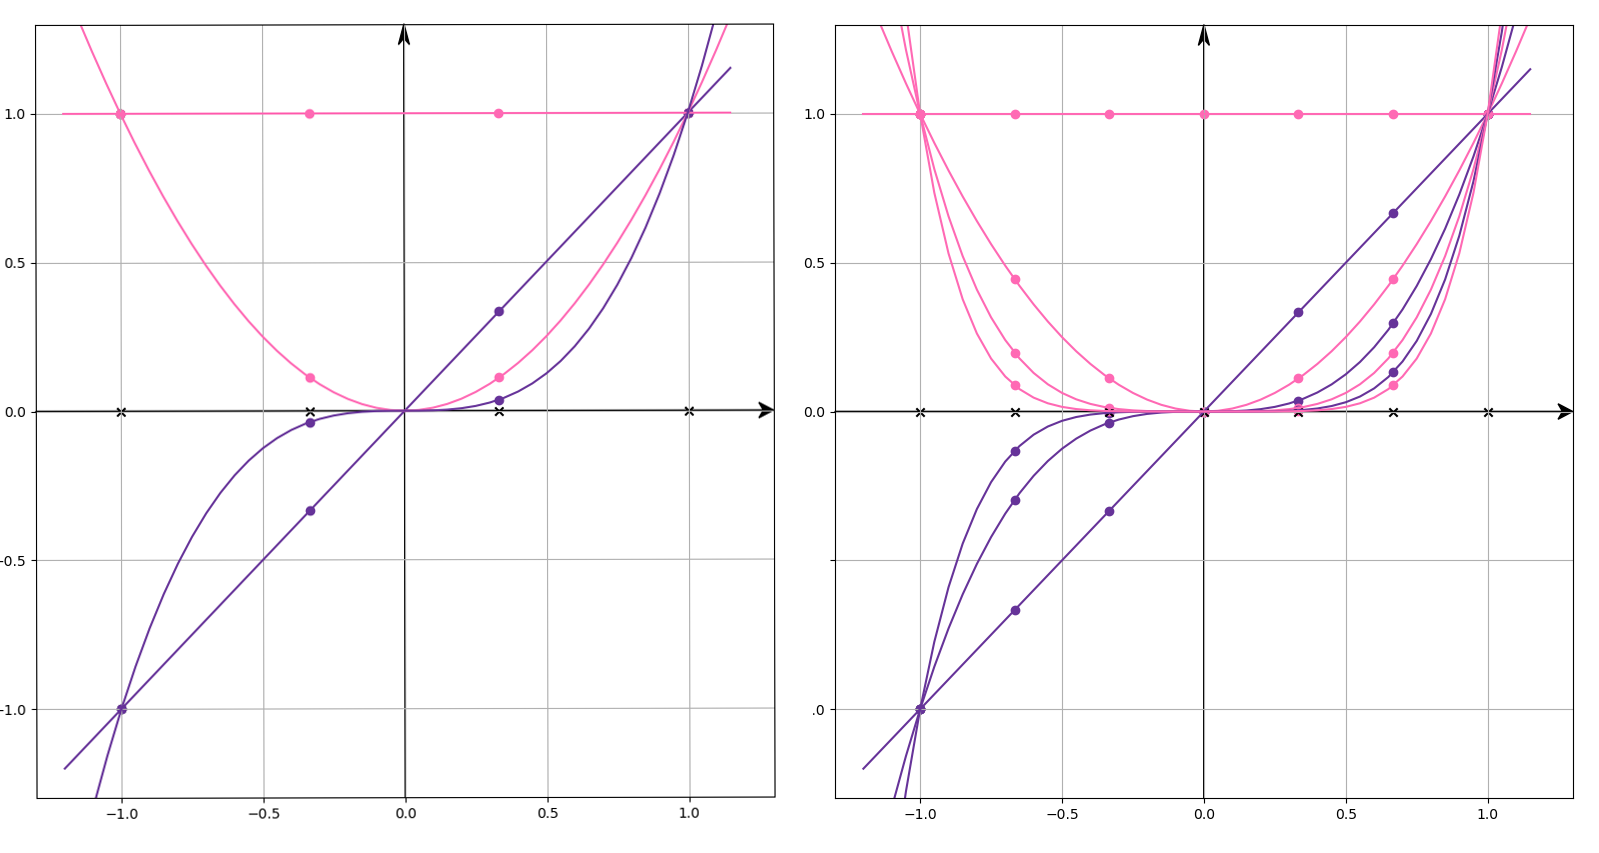
\includegraphics[scale=0.28]{10Dic_1} 
\end{figure}	

Antes de empezar nuestro análisis, damos definiciones
para las simetrías que parecen aparecer en las entradas
de los polinomios discretos de Legendre.

\begin{marginfigure}
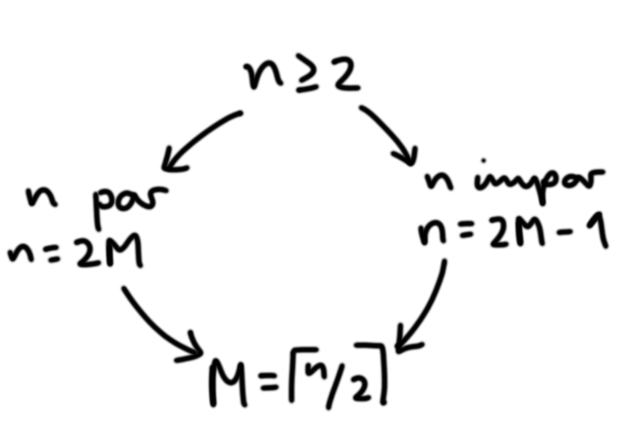
\includegraphics[scale=0.7]{n_parImpar} 
\end{marginfigure}


\begin{defi}
\label{def: espacios de seniales simetricas y antisimetricas}
Sea $n \in \IN$, $n \geq 2$. 
Sea $M = \lceil \frac{n}{2} \rceil$.
Definimos al 
\textbf{espacios de señales antisimétricas} $S_{n,-}$ como 
	\begin{equation}
	\label{eq1: 5Dic}
	S_{n, -}:= \{ x=(x_{m})_{m=0}^{n-1}  \in \IR^{n}
	\hspace{0.2cm} |
	\hspace{0.2cm} \forall  
	\hspace{0.1cm}
	0 \leq m \leq M-1 : \hspace{0.2cm} x_{m}= -x_{n-m-1}\}
	\end{equation}

\noindent	
y, además, definimos al
\textbf{espacios de señales simétricas} $S_{n,+}$ como sigue:

\begin{itemize}
	\item si $n$ es par, 
	\begin{equation}
	\label{eq0: 5Dic}
	S_{n, +}:= \{ x=(x_{m})_{m=0}^{n-1} \in \IR^{n} \hspace{0.2cm} 
	| \hspace{0.2cm} \forall  
	\hspace{0.1cm}
	0 \leq m \leq M-1 : \hspace{0.2cm} x_{m}= x_{n-m-1}\},
	\end{equation}
	y,
	
	\item si $n$ es impar,
	\begin{equation}
	\label{eq0: 5Dic}
	S_{n, +}:= \{ x=(x_{m})_{m=0}^{n-1} \in \IR^{n} \hspace{0.2cm} 
	| \hspace{0.2cm} \forall  
	\hspace{0.1cm}
	0 \leq m \leq M-2 : \hspace{0.2cm} x_{m}= x_{n-m-1}\},
	\end{equation}
	
\end{itemize}
\end{defi}


\begin{figure}[H]
	\sidecaption{
	Figura que ilustra las definiciones de los
	espcios $S_{n,+}$ y $S_{n,-}$ para distintas paridades
	de $n$.
	\label{fig: sim_antisim}
	}
	\centering
	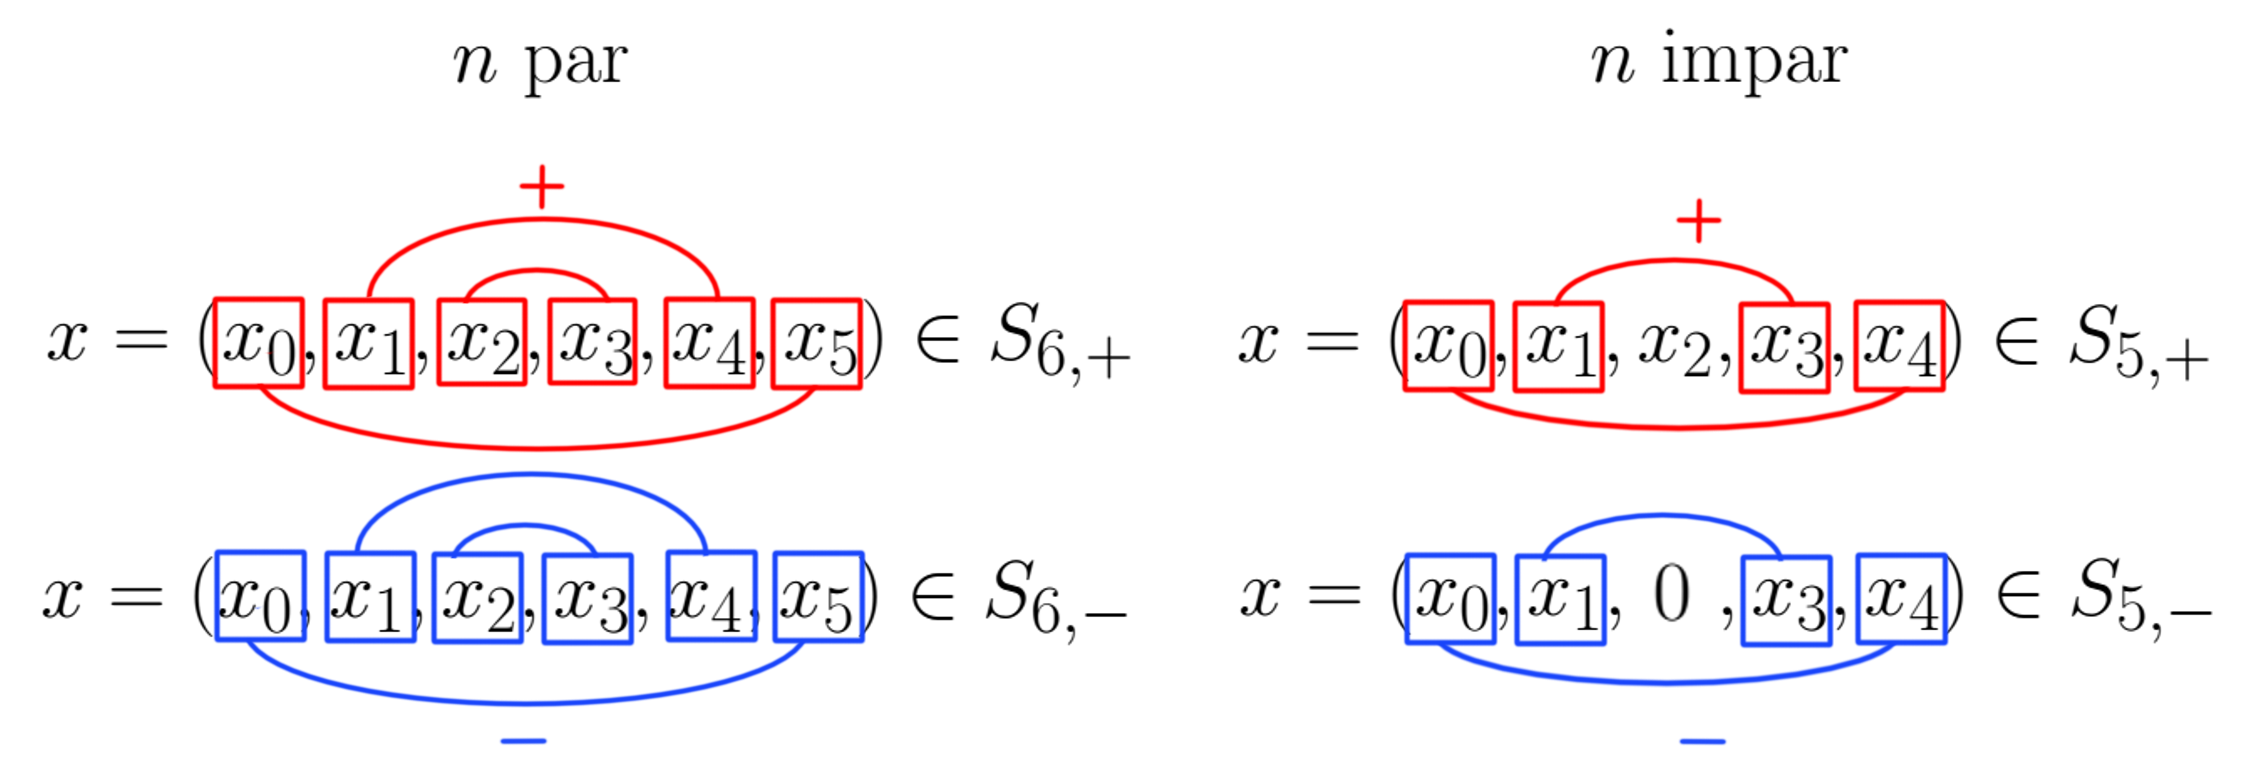
\includegraphics[scale=0.8]{sim_antisim} 
\end{figure}	

Las siguientes dos observaciones se siguen de inmediato.
\begin{obs}
\label{obs: espacios de senales sim y antisim}
Sea $n \geq 2$ entero.  
Los conjuntos $S_{n,+}$ y $S_{n,-}$ definidos como en  
\ref{def: espacios de seniales simetricas y antisimetricas}. 
son subespacios de $\IR^{n}$.
\end{obs}

\begin{obs}
\label{obs: pertenencia}
Sea $n \geq 2$ entero.  
Sea $\cali{P}$ la malla
uniforme de $n$ puntos con puntos extremos $-1$ y $1$.
Para toda $0 \leq k \leq n-1$, sean
las potencias básicas $f_{k}(t)=t^{k}$ y los vectores
\begin{equation}
\label{eq4: 10Dic}
w_{k}=(w_{k,m})_{m=0}^{n-1} := \Omega_{n, \cali{P}}(f_{k}),
\end{equation}
donde $\Omega_{n, \cali{P}}$ es el operador definido en 
\ref{def: operador de discretizacion puntual}.
Para toda $0 \leq k \leq n-1$ se tiene que
\begin{itemize}
\item $w_{k} \in S_{n,+}$ si $k$ es par, y
\item $w_{k} \in S_{n,-}$ si $k$ es impar,
\end{itemize}
donde $S_{n,+}$ y $S_{n,-}$ son como en 
\eqref{eq0: 5Dic} y \eqref{eq2: 19En}.
\end{obs}

Es fácil establecer la perpendicularidad entre
señales simétricas con señales antisimétricas.
Hacemos esto a continuación

\begin{lema}
\label{lema: ortogonalidad entre sim y antisim}
Sea $n \geq 2$.
Sean $S_{n,+}$ y $S_{n,-}$ como en la definición
\ref{def: espacios de seniales simetricas y antisimetricas}.
Para cualesquiera 
$u \in S_{m,+}$ y $v \in S_{n,-}$ se tiene que
$\langle u, v \rangle=0$.
\end{lema}
\noindent
\textbf{Demostración.}
Supongamos que $n$ es impar; digamos entonces que
$n = 2M-1$, 
\begin{equation*}
u=(a_{0}, \ldots , a_{M-2}, a_{M-1}, a_{M-2}, \ldots a_{0}),
\end{equation*}
y que 
\begin{equation*}
v=(b_{0}, \ldots , b_{M-2}, 0, -b_{M-2}, \ldots -b_{0}).
\end{equation*}
Se calcula directamente que 

\[
\langle u, v \rangle = \suma{m=0}{M-2}{a_{m} \cdot b_{m}} + a_{N} \cdot 0
-\suma{m=0}{M-2}{a_{m} \cdot b_{m}} =0.
\]

\noindent
El argumento para $n$ par es análogo.
\QEDB
\vspace{0.2cm}

\subsection{Estudio para dimensiones impares}
A lo largo de esta subsección vamos 
estudiar las simetrías presentes en las entradas
de los PDL $\cali{L}^{n,k}$, con $0 \leq k \leq n-1$
cuando la dimensión $n$ es impar;
$n \in \IN$ impar; digamos que

\begin{equation}
\label{eq1: 19En}
n=2M - 1 \hspace{0.2cm} \text{ con } M \in \IN.
\end{equation}

\begin{teo}
\label{prop: simetrias en dimensiones impares}
\textbf{(Sobre simetrías
en los polinomios discretos de Legendre de dimensión impar)}. 
Sea $n \in \IN$ como en \eqref{eq1: 19En}.
Sea $0 \leq k \leq n-1$ y
considere al vector $\cali{L}^{n,k}=(\cali{L}^{n,k}_{m})_{m=0}^{n-1}$
como se ha definido en \eqref{def: base de Legendre discreta}. 
Se tiene que 
\begin{itemize}
\item $\cali{L}^{n,k} \in S_{n,+}$ si $k$ es par, y que
\item $\cali{L}^{n,k} \in S_{n,-}$ si $k$ es impar,
\end{itemize}
es decir, que para toda $0 \leq m \leq N-1$ 
\begin{itemize}
\item para toda $0 \leq m \leq M-2$ se tiene que 
$\cali{L}^{n,k}_{m} = \cali{L}^{n,k}_{n-m-1}$ si $k$ es par y
\item para toda $0 \leq m \leq M-2$ 
se tiene que $\cali{L}^{n,k}_{m} = -\cali{L}^{n,k}_{2N-m}$ y 
$\cali{L}^{n, k}_{M-1}=0$ si $k$ es impar.
\end{itemize}
\end{teo}
\begin{figure}[H]
\centering\captionsetup{format = hang}
	\begin{measuredfigure}
		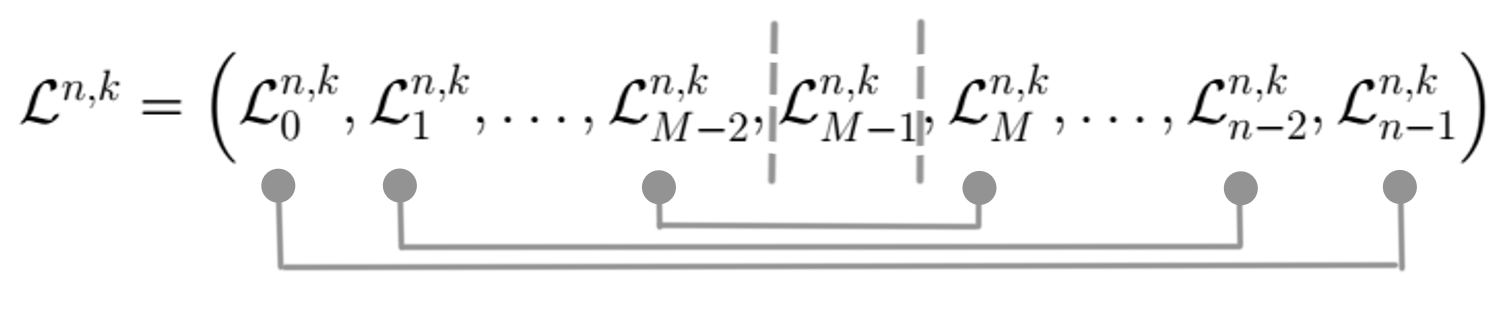
\includegraphics[scale=0.7]{simetria1} 
		\caption{
		\TODO{Corregir!!}		
		Fijadas una dimensión impar $n=2N+1$ 
		y un grado $0 \leq k \leq n-1$,
		en esta proposición se da una relación simple entre las parejas 
		de entradas de $\cali{L}^{n,m}$ con índices $m$ y $2N-m$ 
		(donde los índices $0 \leq m \leq N-1$ son los de las primeras
		$N$ entradas).}
 	\end{measuredfigure}
 \end{figure}

\noindent
\textbf{Demostración.}
Sean los vectores $w_{k}$ como en la observación 
\ref{obs: pertenencia}.
Según lo demostrado en la subsección \TODO{ref}, si
\[
\{ \overline{\eta}_{k} : \hspace{0.2cm} 0 \leq k \leq n-1 \}
\]
es la base de $\IR^{n}$ que se obtiene al ortogonalizar 
con el proceso de Gram-Schmidt a la base
\[
\{ w_{k} : \hspace{0.2cm} 0 \leq k \leq n-1 \}
\]
de $\IR^{n}$,
o sea, si 

\begin{equation}
\label{eq3: 19En}
\overline{\eta}_{0}= w_{0},
\end{equation}
y si

\begin{equation}
\label{eq3: 19En}
\forall \hspace{0.1cm} 1 \leq k \leq n-1: 
\hspace{0.2cm}
\overline{\eta}_{k}= w_{k}-
\suma{j=0}{k-1}{
\frac{\langle w_{k}, \overline{\eta}_{j} \rangle}
{\langle \overline{\eta}_{j}, \overline{\eta}_{j} \rangle}\overline{\eta}_{j},
}
\end{equation}


\noindent
entonces, para toda $0 \leq k \leq n-1$ tenemos la relación 
\[
\cali{L}^{n,k}= \frac{1}{||\overline{\eta}_{k}||} \cdot \overline{\eta}_{k};
\]
en particular, los vectores $\cali{L}^{n,k}$ y 
$\overline{\eta}_{k}$ son múltiplos escalares uno del otro.

Afirmamos que ocurre que
$\overline{\eta}_{k} \in S_{+}$ (resp. que
$\overline{\eta}_{k} \in S_{-,0}$) si $k$ es par
(resp. impar); por ser $S_{+}$
y $S_{-,0}$ cerrado bajo multiplicación
por escalares (c.f. observación 
\ref{obs: espacios de senales sim y antisim}),
si logramos demostrar esta afirmación podremos concluir lo deseado.


Procedemos a demostrar esto por inducción sobre $k$.

\begin{itemize}

\item (Base de inducción) según la igualdad
\eqref{eq3: 19En} y la observación 
\ref{obs: pertenencia}, la afirmación 
es trivialmente cierta para $k=0$, el menor grado par.
Considere ahora a $k=1$, el menor grado impar. Según 
\eqref{eq3: 19En}, 
\begin{equation}
\label{eq5: 19En}
\overline{\eta}_{1}= w_{1}
- \frac{\langle w_{1}, \overline{\eta}_{0} \rangle}
{\langle \overline{\eta}_{0}, \overline{\eta}_{0} \rangle}\overline{\eta}_{0};
\end{equation}
De la observación 
\ref{obs: pertenencia} y el lema
\ref{lema: ortogonalidad entre sim y antisim} se sigue
que el producto punto $\langle w_{1}, \overline{\eta}_{0} \rangle$
es cero; sustituyendo esto en \eqref{eq5: 19En}
se infiere que 
\[
\overline{\eta}_{1} = w_{1} + 0 \cdot \overline{\eta}_{0}=
w_{1} \in S_{-}.
\]
Digamos pues que

\[
\overline{\eta}_{1} = 
(a_{0}, \ldots , a_{N-1}, a_{N}, -a_{N-1}, \ldots , -a_{0} );
\]
para completar la base de inducción debemos de mostrar
que $a_{N}$, la entrada central de $\overline{\eta}_{1}$,
es cero. Según \eqref{eq2: 19En} y
la definición del polinomio discreto $w_{0}$, 
$\overline{\eta}_{0}$ es el vector constante uno de $\IR^{n}$;
ahora bien, puesto que $\overline{\eta}_{0}$
y $\overline{\eta}_{1}$
son ortogonales entre sí, llegamos, como queríamos, a que

\[
0 = \langle \overline{\eta}_{0}, \overline{\eta}_{1}\rangle
= \suma{m=0}{n-1}{a_{m}} = 
\suma{m=0}{N-1}{a_{m}} +a_{N} -
\suma{m=0}{N-1}{a_{m}} = a_{N}.
\]



\item (Paso inductivo) sea $0 \leq k \leq n-1$ par, y
supongamos la afirmación cierta para todo polinomio de Legendre
discreto de dimensión $n$ y grado menor a $k$;
mostremos que $\overline{\eta}_{k}$ es elemento de $S_{+}$.
La fórmula \eqref{eq3: 19En} nos da una expresión
para $\overline{\eta}_{k}$.
Puesto que
para toda $0 \leq j \leq k-1$ impar se tiene 
(por hipótesis de inducción) 
que $\overline{\eta}_{j} \in S_{-,0}$
y como $w_{k} \in S_{+}$ (c.f. observación 
\ref{obs: pertenencia}), tenemos, según el lema
\ref{lema: ortogonalidad entre sim y antisim}, que
para todo $0 \leq j \leq k-1$ impar, 
$\langle w_{k}, \overline{\eta}_{j} \rangle=0$;
sustituyendo esto en la expresión para 
$\overline{\eta}_{k}$, llegamos a que
\begin{equation}
\label{eq3: 19En}
\forall \hspace{0.1cm} 1 \leq k \leq n-1: 
\hspace{0.2cm}
\overline{\eta}_{k}= w_{k}-
\suma{
\substack{ {j=0}, \\  {j\text{ par}}}
}{k-1}{
\frac{\langle w_{k}, \overline{\eta}_{j} \rangle}
{\langle \overline{\eta}_{j}, \overline{\eta}_{j} \rangle}\overline{\eta}_{j}
};
\end{equation}
según la observación \ref{obs: pertenencia}
y nuestra hipótesis de inducción, 
\eqref{eq3: 19En} expresa al vector 
$\overline{\eta}_{k}$ como combinación lineal
de elementos de $S_{+}$, luego, lo expone como
elemento de este espacio vectorial. De un argumento
dual se sigue la veracidad de la afirmación también
cuando se supone $k$ impar.
\end{itemize}
\QEDB
\vspace{0.2cm}

\subsection{Estudio para dimensiones pares}
Una discusión análoga a la desarrollada en la subsección
anterior se sigue para cuando la dimensión $n$ de espacio
es par; la única diferencia es que los vectores discretos
de Legendre de una tal dimensión no tienen entrada central,
pero los argumentos de simetría y antisimetría se siguen
igualmente.

Establecemos pues, sin demostración, 
la contraparte del teorema
\ref{prop: simetrias en dimensiones impares} 
correspondiente a dimensiones pares.


\begin{teo}
\label{prop: simetrias en dimensiones pares}
\textbf{(Para dimensiones pares)}. Sea $n \in \IN$ par, digamos,

$n=2N$, con $N \geq 1$. Sea $0 \leq k \leq n-1$ y
considere al vector $\cali{L}^{n,k}=(\cali{L}^{n,k}_{m})_{m=0}^{n-1}$
como se ha definido en \eqref{def: base de Legendre discreta}.
Para toda $0 \leq m \leq N-1$ se tiene que
\begin{itemize}
\item $\cali{L}^{n,k}_{m} = \cali{L}^{n,k}_{2N-m-1}$ si $k$ es par y
\item $\cali{L}^{n,k}_{m} = -\cali{L}^{n,k}_{2N-m-1}$ si $k$ es impar.
\end{itemize}
\end{teo}
\begin{figure}[H]
\centering\captionsetup{format = hang}
	\begin{measuredfigure}
		\includegraphics[scale=1.3]{simetria2} 
		\caption{Fijadas una dimensión par $n=2N$ 
		y un grado $0 \leq k \leq n-1$,
		en esta proposición se da una relación simple entre las parejas 
		de entradas de $\cali{L}^{n,m}$ con índices $m$ y $2N-m-1$ 
		(donde los índices $0 \leq m \leq N-1$ son los de las primeras
		$N$ entradas).}
 	\end{measuredfigure}
 \end{figure}

Gracias a lo demostrado en esta sección, sabemos que,
fijada una dimensión $n$ y fijado un grado $0 \leq k \leq n-1$,
el cálculo de las $n$ entradas del vector $\cali{L}^{n,k}$
se reduce al cálculo de la mitad de estas, pues las otras pueden
deducirse de las primeras con un cambio de signo que está completamente
determinado por la paridad del grado $k$.


\begin{figure}[H]
\centering\captionsetup{format = hang}
	\begin{measuredfigure}
		\includegraphics[scale=1]{10Dic_3} 
		\caption{\TODO{aaa}}
 	\end{measuredfigure}
 \end{figure}

\section{Implementación computacional de las bases discretas de Legendre}
\label{Implementación computacional de las bases discretas de Legendre en Python}

Haciendo uso de
la fórmula establecida en el teorema
\ref{teo: expresión analítica de BON de Legendre}
y las simetrías exploradas en el capítulo
\ref{section: sobre simetrias en las entradas de los poliomios discretos de Legendre}, definiremos un
algoritmo para calcular
las bases de Legendre discretas. Para implementarlo, lo escribiremos
en Python. 
El input y output del algoritmo deseado son como siguen:


\begin{itemize}
\item \textbf{Input}: la dimensión requerida $n \geq 2$, variable
de tipo \code{int}. 
\item \textbf{Output}: lista con $n$ entradas,
siendo la $k-$ésima entrada (con $0 \leq k \leq n-1$)
una lista que contiene las $n$ entradas del
vector $\cali{L}^{n,k}$.
\end{itemize}

\begin{figure}[H]
	\sidecaption{
		Se ilustran el input y el output
		esperados del algoritmo para $n=5$. En los scripts
		que escribimos no se pidió redondeo a cuatro decimales.
	\label{fig: input y output deseados}
	}
	\centering
	\includegraphics[scale=0.7]{7En_1} 
\end{figure}	

\subsection{Análisis de la expresión de los PDL}
Sean $n \in \IN$, $0 \leq k \leq n-1$.
Veamos cómo usar lo que sabemos para calcular eficientemente
al vector $\cali{L}^{n,k}$ o, equivalentemente, para calcular
cada una de sus $n$ entradas, que son los números reales
$\cali{L}^{n,k}_{m}$, con $0 \leq m \leq n-1$.

Conviene reescribir la expresión
\eqref{eq0: 6En} resaltando con colores el papel que juegan
la dimensión $n$, el grado $k$ y la posición $m$ en la fórmula
para $\cali{L}^{n,k}_{m}$:

\begin{equation}
\label{eq1: 6En}
\cali{L}^{
{\color{ameCyanO}{n}},{\color{ameVerde}{k}}}_{\color{ameGris}{m}}= 
(-1)^{{\color{ameVerde}{k}}} 
\sqrt{\frac{(2
{\color{ameVerde}{k}}+1)(
{\color{ameCyanO}{n}}-1)^{(
{\color{ameVerde}{k}})}}{(
{\color{ameCyanO}{n}}+
{\color{ameVerde}{k}})^{(
{\color{ameVerde}{k}}+1)}}}
\suma{j=0}{
{\color{ameVerde}{k}}}{(-1)^{j}\binom{
{\color{ameVerde}{k}}}{j}\binom{
{\color{ameVerde}{k}}+j}{j}
\frac{{\color{ameGris}{m}}^{(j)}}{(
{\color{ameCyanO}{n}}-1)^{(j)}}}.
\end{equation}

Recuerde el concepto de fading factorial
definido en \ref{def: fading factorial}.
Observe ahora que, en la expresión \eqref{eq1: 6En},
aparecen cuatro fading factorials;
\begin{itemize}
\item $(n-1)^{(k)}$, que nunca es cero, pues $n-1 \geq k$
siempre ocurre,
\item $(n+k)^{(k+1)}$, que nunca es cero, pues $n+k \geq k+1$
siempre ocurre,
\item $(n-1)^{(j)}$ que, por ocurrir $j \leq k \leq n-1$, 
nunca es cero, y
\item $m^{(j)}$, que no es cero si y sólo si $j \leq m$;
\end{itemize}
según este último punto, algunos de los sumandos
considerados en la sumatoria 
en \eqref{eq1: 6En} pueden ser cero; podemos
ajustar el limite superior de la sumatoria y llegar así a que
\begin{equation}
\label{eq2: 6En}
\cali{L}^{
{\color{ameCyanO}{n}},{\color{ameVerde}{k}}}_{\color{ameGris}{m}}= 
(-1)^{{\color{ameVerde}{k}}} 
\sqrt{\frac{(2
{\color{ameVerde}{k}}+1)(
{\color{ameCyanO}{n}}-1)^{(
{\color{ameVerde}{k}})}}{(
{\color{ameCyanO}{n}}+
{\color{ameVerde}{k}})^{(
{\color{ameVerde}{k}}+1)}}}
\suma{j=0}{
min(
{\color{ameVerde}{k}},
{\color{ameGris}{m}})
}{
{(-1)^{j}\binom{
{\color{ameVerde}{k}}}{j}\binom{
{\color{ameVerde}{k}}+j}{j}
\frac{{\color{ameGris}{m}}^{(j)}}{(
{\color{ameCyanO}{n}}-1)^{(j)}}}.
},
\end{equation}

Podemos también usar la definición de fading factorial
para reescribir \eqref{eq2: 6En}
en términos de factoriales
como sigue:


\begin{equation}
\label{eq5: 6En}
\cali{L}^{
{\color{ameCyanO}{n}},{\color{ameVerde}{k}}}_{\color{ameGris}{m}}= 
A_{
{\color{ameCyanO}{n}},
{\color{ameVerde}{k}}
}
\suma{j=0}{
min(
{\color{ameVerde}{k}},
{\color{ameGris}{m}})}
{B_{
{\color{ameCyanO}{n}},
{\color{ameVerde}{k}},
{\color{ameGris}{m}},j
}
},
\end{equation}
donde

\begin{equation}
\label{eq3: 6En}
A_{
{\color{ameCyanO}{n}},
{\color{ameVerde}{k}}
}:=
(-1)^{{\color{ameVerde}{k}}} 
({\color{ameCyanO}{n}}-1)!
\sqrt{\frac{(2
{\color{ameVerde}{k}}+1)}
{(
{\color{ameCyanO}{n}}-
({\color{ameVerde}{k}}+1))!
(
{\color{ameCyanO}{n}} + {\color{ameVerde}{k}}
)!
}},
\end{equation}
y

\begin{equation}
\label{eq4: 6En}
B_{
{\color{ameCyanO}{n}},
{\color{ameVerde}{k}},
{\color{ameGris}{m}},j
}:=
(-1)^{j}
\frac{
{\color{ameGris}{m}}!
}{
({\color{ameCyanO}{n}}-1)!
}
\frac{
({\color{ameVerde}{k}} + j) !
({\color{ameCyanO}{n}}-(j+1))!
}{
(j!)^{2}
({\color{ameVerde}{k}}-j)!
({\color{ameGris}{m}}-j)!
}.
\end{equation}



Usando las fórmulas \eqref{eq5: 6En}, 
\eqref{eq3: 6En} y \eqref{eq4: 6En} junto con las
simetrías estudiadas en la sección 
\ref{section: sobre simetrias en las entradas de los poliomios discretos de Legendre}, podemos escribir con facilidad el algoritmo deseado.

\section{Pseudocódigos algoritmos usados para calcular las BDL}
A continuación mostramos los pseudocódigos para calcular 
los polinomios discretos de Legendre.

Las implementaciones en Python de todos estos algoritmos
se compartieron en \TODO{referencia.}

\begin{itemize}
\item Damos los algoritmos \textbf{sumandoV1} y 
\textbf{sumandoV2} (c.f. \ref{alg: sumandoV1},
\ref{alg: sumandoV2}) para calcular el número
\begin{equation}
\label{eq0: 1Abril}
B_{n, k, m, j}.
\end{equation}
El primero usa directamente la fórmula \eqref{eq4: 6En},
mientras que en el segundo 
simplificamos los factoriales que
aparecen en la definición \eqref{eq4: 6En}
de $B_{n,k,m,j}$
para llegar a la expresión
\[
(-1)^{j}
\frac{m!}{(n-1)!}
 \frac{(k+j)!(n-j-1)!}{(j!)^{2}(k-j)!(m-j)!}
= (-1)^{j}
\frac{\left( \producto{\mu=m-j+1}{m}{\mu} \right)
\left( \producto{\mu=k-j+1}{k+1}{\mu} \right)
}{
\left( \producto{\mu=n-j}{n-1}{\mu} \right)
\left( \producto{\mu=n-j}{n-1}{\mu} \right)^{2}
}.
\] 

\item Damos dos algoritmos \textbf{sumatoriaV1}
y \textbf{sumatoriaV2} (c.f. \ref{alg: sumatoriaV1}
y c.f. \ref{alg: sumatoriaV2}) para calcular a la suma
\begin{equation}
\label{eq1: 1Abril}
\suma{j=0}{min(k,m)}{B_{n, k, m, j}};
\end{equation}
observe en la definición de estos que 
\textbf{sumatoriaV1} hace referencia a
\textbf{sumandoV1}, mientras que \textbf{sumatoriaV2}
hace referencia a \textbf{sumandoV2}


\item Los algoritmos 
\textbf{baseLegendre$\_$dimImpar} y
\textbf{baseLegendre$\_$dimPar} 
(c.f. \ref{alg: legendre impar} y \ref{alg: legendre par} )
que sirven para calcular, usando ya sea el algoritmo
\textbf{sumatoriaV1} o \textbf{sumatoriaV2},
la base de Legendre discreta de dimensión $n$; se usa el primero
si $n$ es impar y el segundo si $n$ es par.
Las lineas 10 de estos 
algoritmos se justifican,
respectivamente, con los teoremas 
\ref{prop: simetrias en dimensiones impares}
y \ref{prop: simetrias en dimensiones pares}.
Por último, tenemos el sencillo algoritmo \textbf{calculo$\_$base},
que, en base a la paridad de la dimensión $n$, decide si usar
el algoritmo \ref{alg: legendre impar} o el \ref{alg: legendre par}
para calcular la BDL de dimensión $n$.
\end{itemize}

Para los pseudocódigos usamos las siguiente abreviaciones:

\begin{itemize}
	\item \textit{APPEND(A,t)} donde $A$ es una lista y $t$ es un elemento
	significa ``agregar $t$ al final de la lista $A$''.
	\item \textit{CONCATENATE(A,B)}, donde $A$ y $B$ son listas, significa
	concatenar $A$ con $B$.
	\item \textit{PRODUCT(A)}, donde $A$ es una lista cuyas entradas
	son todas variables de tipo \code{float}, significa ``calcular el producto
	de todos los elementos de $A$''. Si $A$ es vacía, $PRODUCT(A)$ es uno.
	\item \textit{SUM(A)}, donde $A$ es una lista cuyas entradas
	son todas variables de tipo \code{float}, significa ``calcular la suma
	de todos los elementos de $A$''. 
	\item \textit{CEIL(a)}, donde $a$ es una variable de tipo \code{float}, significa
	``calcular $\lceil a \rceil$''.
\end{itemize}

\begin{algorithm}
\caption{$sumandoV1$}\label{alg: sumandoV1}
\begin{algorithmic} [1]
\REQUIRE $n$, $k$, $m$, $j$, todas de tipo int, con $n \geq 2$, 
$0 \leq k, m \leq n-1$, $0 \leq j \leq min(k,m)$
\ENSURE El número $B_{n, k, m, j}$ definido en \eqref{eq0: 1Abril}.
\RETURN $\frac{(k+j)! * (n-j-1)! }{(j!)^{2}* (k-j)! * (m-j)!}$
\end{algorithmic}
\end{algorithm}

\begin{algorithm}
\caption{$sumandoV2$}\label{alg: sumandoV2}
\begin{algorithmic} [1]
\REQUIRE $n$, $k$, $m$, $j$, todas de tipo int, con $n \geq 2$, 
$0 \leq k, m \leq n-1$, $0 \leq j \leq min(k,m)$
\ENSURE El número \eqref{eq0: 1Abril}
\STATE $B1, B2, B3, B4 \leftarrow [\hspace{0.2cm}]$
\FOR {$t=m-j+1$ \textbf{to} $t=m$} 
\STATE $APPEND(B1, t)$
\ENDFOR
\FOR {$t=k-j+1$ \textbf{to} $t=k+j$} 
\STATE $APPEND(B2, t)$
\ENDFOR
\FOR {$t=n-j$ \textbf{to} $t=n-1$} 
\STATE $APPEND(B3, t)$
\ENDFOR
\FOR {$t=1$ \textbf{to} $t=j$} 
\STATE $APPEND(B4, t)$
\ENDFOR
\STATE $num \leftarrow CONCATENATE(B1, B2)$
\STATE $den \leftarrow CONCATENATE(B3, B4)$
\STATE $den \leftarrow CONCATENATE(den, B4)$
\STATE $numerador = PRODUCT(num)$
\STATE $denominador = PRODUCT(den)$
\RETURN $numerador/denominador$
\end{algorithmic}
\end{algorithm}



\begin{algorithm}
\caption{$sumatoriaV1$}\label{alg: sumatoriaV1}
\begin{algorithmic} [1]
\REQUIRE $n$, $k$, $m$, todas de tipo int, con $n \geq 2$, 
$0 \leq k, m \leq n-1$, $0 \leq j \leq min(k,m)$
\ENSURE La suma $\suma{j=0}{min(k,m)}{B_{n, k, m, j}}$

\STATE $limite \leftarrow minimo(m,k)$
\STATE $factor \leftarrow \frac{m!}{(n-1)!}$
\STATE $sumandos\_pares \leftarrow [ \hspace{0.2cm} ]$
\STATE $sumandos\_impares \leftarrow [ \hspace{0.2cm}]$
\FOR {$j=0$ \textbf{to} $j=limite$} 
\IF{$j \equiv 1 \hspace{0.1cm} (mod \hspace{0.1cm} 2)$}
\STATE $APPEND$($sumandos\_impares$, $sumandoV1(n,k,m,j)$)
\ELSE
\STATE $APPEND$($sumandos\_pares$, $sumandoV1(n,k,m,j)$)
\ENDIF
\ENDFOR
\STATE $suma\_pares \leftarrow SUM(sumandos\_pares)$
\STATE $suma\_impares \leftarrow SUM(sumandos\_impares)$
\RETURN $factor * (suma\_pares - suma\_impares)$
\end{algorithmic}
\end{algorithm}

\begin{algorithm}
\caption{$sumatoriaV2$}\label{alg: sumatoriaV2}
\begin{algorithmic} [1]
\REQUIRE $n$, $k$, $m$, todas de tipo int, con $n \geq 2$, 
$0 \leq k, m \leq n-1$, $0 \leq j \leq min(k,m)$
\ENSURE La suma $\suma{j=0}{min(k,m)}{B_{n, k, m, j}}$

\STATE $limite \leftarrow minimo(m,k)$
\STATE $sumandos\_pares \leftarrow [ \hspace{0.2cm} ]$
\STATE $sumandos\_impares \leftarrow [\hspace{0.2cm} ]$
\FOR {$j=0$ \textbf{to} $j=limite$} 
\IF{$j \equiv 1 \hspace{0.1cm} (mod \hspace{0.1cm} 2)$}
\STATE $APPEND$($sumandos\_impares$, $sumandoV2(n,k,m,j)$)
\ELSE
\STATE $APPEND$($sumandos\_pares$, $sumandoV2(n,k,m,j)$)
\ENDIF
\ENDFOR
\FOR {$j=0$ \textbf{to} $j=limite$ \textbf{and} $j$ \textbf{odd}} 
\STATE $APPEND$($sumandos\_impares$, $sumandoV2(n,k,m,j)$)
\ENDFOR
\STATE $suma\_pares \leftarrow SUM(sumandos\_pares)$
\STATE $suma\_impares \leftarrow SUM(sumandos\_impares)$
\RETURN $suma\_pares - suma\_impares$
\end{algorithmic}
\end{algorithm}


%-----------------------------------------------------------------

\begin{algorithm}
\caption{base$\_$legendre$\_$dimImpar}\label{alg: legendre impar}
\begin{algorithmic}[1] 
\REQUIRE $n$, variable de tipo int, $n \geq 2, \hspace{0.1cm} n \equiv 1 \hspace{0.1cm} (mod \hspace{0.1cm} 2)$, 'sumatoria' es una de las dos funciones definidas en los algoritmos
\ref{alg: sumatoriaV1} y \ref{alg: sumatoriaV2}.
\ENSURE lista cuyos elementos son $n$ listas, conteniendo
la $k-$ésima lista las $n$ entradas del polinomio discreto de Legendre de
grado $k$ y dimensión $n$.
%\ENSURE $y = x^n$
\STATE $M \leftarrow CEIL(n/2)$
\STATE $base\_legendre=[ \hspace{0.2cm} ]$ 
\STATE $signo \leftarrow 1$ 
\FOR {$k=0$ \textbf{to} $k=n-1$} 
\STATE $A\_nk \leftarrow signo * (n-1)!*
\sqrt{\frac{
2k+1
}{
(n-k-1)!*(n+k)!
}}$

\STATE $vector\_legendre \leftarrow [ 0, \ldots , 0]$ \COMMENT{Lista con $n$ ceros} 
\FOR {$m=0$ \textbf{to} $m=M-2$} 
\STATE $entrada \leftarrow A\_nk * sumatoria(n,k,m)$
\STATE $vector\_legendre[m] \leftarrow entrada$ 
\STATE $vector\_legendre[n-m-1] \leftarrow signo*entrada$ 
\ENDFOR

\IF{$k \equiv 1 \hspace{0.1cm} (mod \hspace{0.1cm} 2)$}
\STATE $vector\_legendre[M-1] \leftarrow 0$
\ELSE
\STATE $vector\_legendre[M-1] \leftarrow A\_nk * sumatoria(n,k,M-1)$
\ENDIF
\STATE $APPEND(base\_legendre, vector\_legendre)$
\STATE $signo \leftarrow signo * -1$
\ENDFOR
\RETURN $base\_legendre$
\end{algorithmic}
\end{algorithm}



\begin{algorithm}
\caption{base$\_$legendre$\_$dimPar}\label{alg: legendre par}
\begin{algorithmic} [1]
\REQUIRE $n$, variable de tipo int, $n \geq 2, \hspace{0.1cm} n \equiv 0 \hspace{0.1cm} (mod \hspace{0.1cm} 2)$, 'sumatoria' es una de las dos funciones definidas en los algoritmos
\ref{alg: sumatoriaV1} y \ref{alg: sumatoriaV2}.
\ENSURE lista cuyos elementos son $n$ listas, conteniendo
la $k-$ésima lista las $n$ entradas del polinomio discreto de Legendre de
grado $k$ y dimensión $n$.


\STATE $M \leftarrow CEIL(n/2)$
\STATE $base\_legendre=[ \hspace{0.2cm} ]$ 
\STATE $signo \leftarrow 1$ 

\FOR {$k=0$ \textbf{to} $k=n-1$} 
\STATE $A\_nk \leftarrow signo * (n-1)!*
\sqrt{\frac{
2k+1
}{
(n-k-1)!*(n+k)!
}}$

\STATE $vector\_legendre \leftarrow [ 0, \ldots , 0]$ \COMMENT{Lista con $n$ ceros} 
\FOR {$m=0$ \textbf{to} $m=M-1$} 
\STATE $entrada \leftarrow A\_nk * sumatoria(n,k,m)$
\STATE $vector\_legendre[m] \leftarrow entrada$ \COMMENT{Agregamos en la $m-$ésima posición}
\STATE $vector\_legendre[n-m-1] \leftarrow signo *entrada\_legendre$
\ENDFOR

\STATE $APPEND(base\_legendre, vector\_legendre)$
\STATE $signo \leftarrow signo * -1$
\ENDFOR
\RETURN $base\_legendre$
\end{algorithmic}
\end{algorithm}



\begin{algorithm}
\caption{calculo$\_$base}\label{alg: legendre}
\begin{algorithmic} [1]
\REQUIRE $n$, variable de tipo int, $n \geq 2$, función ``sumatoria'', que
es una de las dos funciones definidas en los algoritmos
\ref{alg: sumatoriaV1} y \ref{alg: sumatoriaV2}
\ENSURE lista cuyos elementos son $n$ listas, conteniendo
la $k-$ésima lista las $n$ entradas del polinomio discreto de Legendre de
grado $k$ y dimensión $n$.

\IF{$n \equiv 0 \hspace{0.1cm} (mod \hspace{0.1cm} 2)$}
\RETURN $base\_legendre\_dimPar(n, sumatoria)$
\ELSE
\RETURN $base\_legendre\_dimImpar(n, sumatoria)$
\ENDIF
\end{algorithmic}
\end{algorithm}



\chapter{Estudio espectral}
\label{chap: estudio espectral}


\section{Motivación para realizar un estudio espectral de los PDL}
No es difícil convencerse de que las condiciones de ortogonalidad
impuestas en la definición de la base discreta de Legendre
\marginnote{En esta motivación informal, por ``oscilación''
de una señal $x = (x_{m})_{m=0}^{n-1}$
entendemos
tres cambios consecutivos de signo en sus entradas.}
$\cali{L}^{n}$
forzan a las entradas de los polinomios discretos $\cali{L}^{n,k}$
a cambiar más frecuentemente de signo conforme aumenta
el grado $k$, luego, conforme $k$ tiende a $n-1$,
la cantidad de oscilaciones aumenta; revisemos, 
por ejemplo, el caso $n=4$.



\begin{minipage}{0.5\textwidth}
\begin{figure}[H]
\includegraphics[scale=0.25]{oscil1}
\end{figure}
\end{minipage} \hfill
\begin{minipage}{0.45\textwidth}
1.- Por definición,
$\mathcal{L}^{4,0}$ se obtiene al normalizar 
al vector constante uno de $\IR^{4}$, o sea, 

\[
\cali{L}^{4,0} = \left(
\frac{1}{2}, \frac{1}{2}, \frac{1}{2}, \frac{1}{2}
\right).
\]
\end{minipage} 


\begin{minipage}{0.5\textwidth}
2.- La señal $\cali{L}^{4,1} \in \IR^{4}$ es un polinomio discreto de
dimensión 4 y grado 1 que se obtiene exigiendo las
siguientes condiciones

\[
\langle \cali{L}^{4,1} , \cali{L}^{4,0} \rangle=0
\hspace{0.2cm} \text{y} \hspace{0.2cm}
\langle \cali{L}^{4,1} , \cali{L}^{4,1} \rangle=1;
\]
esta primera condición se refleja en que 
las alturas de los puntos de la gráfica de 
$\cali{L}^{4,1}$ deben sumar cero;
esto implica un cambio de signo (y sólo uno,
pues el polinomio es lineal).

\end{minipage} \hfill
\begin{minipage}{0.45\textwidth}
\begin{figure}[H]
\includegraphics[scale=0.3]{oscil2}
\end{figure}
\end{minipage}

\noindent
3.- El vector
$\cali{L}^{4,2} \in \IR^{4}$,
que es un polinomio discreto
de grado $2$, satisface las siguientes
tres condiciones:

\[
\langle \cali{L}^{4,2} , \cali{L}^{4,0} \rangle=0,
\hspace{0.2cm}
\langle \cali{L}^{4,2} , \cali{L}^{4,1} \rangle=0,
\hspace{0.2cm} \text{y} \hspace{0.2cm}
\langle \cali{L}^{4,2} , \cali{L}^{4,2} \rangle=1.
\]
La segunda condición no da información sobre más
requerimientos que deba cumplir
$\cali{L}^{4,2}$, pues,
como $\cali{L}^{4,1} \in S_{n,-}$
y $\cali{L}^{4,2} \in S_{n,+}$
(c.f. teorema 
\ref{prop: simetrias en dimensiones pares}),
ya del lema
\ref{lema: ortogonalidad entre sim y antisim}
se deducía la ortogonalidad de estas señales; 
observe sin embargo que, si las entradas de 
$\cali{L}^{4,2}$ fuesen todas positivas o todas negativas,
entonces no se tendría la ortogonalidad
con la señal constante $\cali{L}^{4,0}$.


\begin{figure}[H]
\includegraphics[scale=0.6]{oscil3}
\end{figure}

4.- Por último, $\cali{L}^{4,3} \in \IR^{4}$ satisface
las siguientes cuatro condiciones: 

\[
\langle \cali{L}^{4,3} , \cali{L}^{4,0} \rangle=0,
\hspace{0.2cm}
\langle \cali{L}^{4,3} , \cali{L}^{4,1} \rangle=0,
\langle \cali{L}^{4,3} , \cali{L}^{4,2} \rangle=0,
\hspace{0.2cm} \text{y} \hspace{0.2cm}
\langle \cali{L}^{4,3} , \cali{L}^{4,3} \rangle=1.
\]

Según los teoremas 
\ref{cor: propiedades importantes de espacios Wi}
y \ref{prop: simetrias en dimensiones pares},
$\cali{L}^{4,3}$ es la discretización de un polinomio
cúbico y además es una señal antisimétrica (en el sentido de la definición
\ref{def: espacios de seniales simetricas y antisimetricas}); dos gráficas de señales que cumplen esto se ilustran abajo:

\begin{figure}[H]
	\includegraphics[scale=0.6]{oscil4}
	\sidecaption{Observe que la señal cúbica de la izquierda tiene
	un sólo cambio de signo, mientras que la de la derecha (que es 
	$\cali{L}^{4,3}$) tiene tres.}
\end{figure}

La señal cúbica de la izquierda, a pesar de 
ser ortogonal a $\mathcal{L}^{4,0}$ y a $\cali{L}^{4,2}$ por 
simetría (c.f. lema
\ref{lema: ortogonalidad entre sim y antisim}), 
definitivamente no puede ser ortogonal
a $\cali{L}^{4,1}$, pues las entradas de estos dos vectores de 
$\IR^{4}$ tienen el mismo signo. Sin embargo, la señal cúbica 
de la derecha (que de hecho es $\cali{L}^{4,3}$) sí cumple el ser
ortogonal a $\cali{L}^{4,1}$ pero, para lograr esto, sus
entradas deben cambiar de signo tres veces. \\


Después de graficar los PDL de otras dimensiones
puede apreciarse que esta tendencia a aumentar el número
de oscilaciones en las gráficas conforme el grado $k$
tiende a $n-1$ (su cota superior)
parece presentarse en todas las dimensiones.
Por ejemplo, abajo se muestran las gráficas de los 
PDL de dimensión $7$.

\begin{figure}[H]
	\centering
	\includegraphics[scale = 0.55]{oscilaciones_dim7} 
\end{figure}	

\section{Hipótesis sobre las oscilaciones de los PDL}

Con el objetivo de analizar la forma
de oscilación de los PDL, nos proponemos
hacer un análisis espectral. Antes
de proceder sistemáticamente, hagamos un análisis empírico.
\begin{figure}[H]
	\sidecaption{
	Con ``sinusoide'' nos referimos a una función 
	continua cuya forma se ilustra en la figura. Este queda
	completamente determinado al fijar una
	\textbf{amplitud}, una \textbf{frecuencia} y un
	\textbf{desfase}, que nosotros preferimos normalizar
	para que sea un número entre $0$ y $1$.
	\label{fig: sinusoide}
	}
	\centering
	\includegraphics[scale = 0.8]{sinusoide} 
\end{figure}	

Pongamos una dimensión de $n = 60$; a continuación,
graficamos los PDL de dimensión $60$ para los primeros grados,
e intentamos aproximar tales gráficas con sinusoides continuos.


\begin{figure}[H]
	\sidecaption{
	Aproximando las gráficas
	de $\cali{L}^{60,0}$ y $\cali{L}^{60,1}$
	con sinusoides. 
	\label{fig: hip_0,1}
	}
	\centering
	\includegraphics[scale = 0.6]{hip_0,1} 
\end{figure}	

\begin{figure}[H]
	\sidecaption{
	Aproximando las gráficas
	de $\cali{L}^{60,2}$ y $\cali{L}^{60,3}$
	con sinusoides. 
	\label{fig: hip_2,3}
	}
	\centering
	\includegraphics[scale = 0.6]{hip_2,3} 
\end{figure}	

\begin{figure}[H]
	\sidecaption{
	Aproximando las gráficas
	de $\cali{L}^{60,4}$ y $\cali{L}^{60,5}$
	con sinusoides. 
	\label{fig: hip_4,5}
	}
	\centering
	\includegraphics[scale = 0.6]{hip_4,5} 
\end{figure}	


Después de dibujar gráficas parecidas para varias dimensiones, 
establecemos la siguiente hipótesis de trabajo.

\begin{hip}
\label{ref: hipotesis}
Sean $n \geq 2$, $0 \leq k \leq n-1$ entero. 
Sea $\cali{L}^{n,k}$ el PDL de dimensión $n$ y grado $k$.
El espectro de $\cali{L}^{n,k}$ se concentra alrededor
de la frecuencia $\omega = k/2$.
\end{hip}

Se ha formulado de forma intencional la hipótesis 
\ref{ref: hipotesis} en términos vagos, para tener libertad
después de definir las herramientas con las que abordaremos el problema
de dar forma concreta a la hipótesis y mejorarla o refutarla con simulaciones
numéricas. \\ 

Observe que, para analizar la presencia de oscilaciones
en las gráficas de las señales, estamos hablando de un ``espectro''.
se cuenta ya con una herramienta clásica para hacer esta clase de análisis,
cuyo producto final es 
una función que
da información sobre
la importancia que cierta frecuencia tiene para
modelar la gráfica analizada. Hablamos de la transformada 
discreta de Fourier, cuyas bases teóricas comentamos en la sección
\ref{sec: TDF},
para usarla posteriormente para hacer un primer análisis espectral. Motivados
por algunas limitaciones de esta herramienta que comentamos más adelante,
nosotros proponemos una alternativa de metodología para realizar un análisis espectral 
en la sección 
\ref{sec: metodologia para realizar un analisis espectral que considere frecuencias arbitrarias}.

Algunos de los espectros así obtenidos se imprimen en
el capítulo
\ref{chap: resultados numericos analisis espectrales}.
El código para calcular tales espectros para cualquier
señal de $\IR^{n}$ se comparte en
\TODO{referencia cuaderno jupyter.}


\section{La transformada discreta de Fourier}
\label{sec: TDF}

En esta sección vamos a dar la definición usual de 
las bases de Fourier complejas y reales, que son
bases ortonormales de $\IC^{n}$ y de $\IR^{n}$ 
\marginnote{Incluimos este capítulo de teoría clásica
por completitud de este trabajo
y para fijar la notación. 
\cite{fourier1} y \cite{fourier2}
son referencias con mucha más información.}
de $\IC^{n}$
y una de $\IR^{n}$ (que llamaremos
``bases de Fourier complejas y reales''),
definidas ambas en términos de discretizaciones de
sinusoides de frecuencias enteras, y que son herramientas
clásicas para hacer lo que comúnmente se denomina
un \textbf{análisis espectral} de señales finitas.


Puesto que la definición de estas herramientas requiere
de algunas nociones del análisis complejo (en particular, de la
definición de la exponencial compleja y de las raíces $n-$ésimas
de la unidad), damos brevemente algunas definiciones y resultados
necesarios para definir las bases de Fourier.


\subsection{La exponencial compleja y raíces $n-$ésimas de la unidad}


La definición de la función exponencial compleja 
tiene diversas motivaciones
(puede consultar algunas de estas en 
\cite{marsden}). Nosotros sólo
damos la definición de esta, así como algunas propiedades
de ella que se usarán en lo que sigue.

\begin{defi}
\label{def: exponencial compleja}
Si $y \in \IR$, entonces por $exp(iy)$ denotamos al número
complejo de módulo uno y argumento $y$, es decir,
\begin{equation}
\label{eq: exponencial 1}
exp(iy) := cos(y) + i sen(y).
\end{equation}
Para todo número complejo $z = a+bi$, definimos 
$exp(z)$ como sigue:
\begin{equation}
\label{eq: exponencial 2}
exp(z) := e^{x}(cos(y) + i sen(y)).
\end{equation}
\end{defi}

\begin{prop}
\label{prop: propiedades exp compleja}
(\textbf{Algunas propiedades de la exponencial compleja}) 
Sean $z_{1}, z_{2} \in \IC$, $\omega \in \IZ$.
	\begin{itemize}
	\item $\frac{exp(z_{1})}{exp(z_{2})} = exp(z_{1} - z_{2})$
	\item $exp(z_{1} + z_{2}) = exp(z_{1}) \cdot exp(z_{2})$
	\item $(exp(z_{1}))^{\omega} = exp(\omega z)$
	\item $exp(z) = 1$ si y sólo si $z= 2K \pi i$ para algún $K \in \IZ$ 
	\item para todo $y \in \IR$, 
	\begin{equation}
	\label{eq: coseno exponenciales}
	cos(y) = \frac{exp(iy)+exp(-iy)}{2}
	\end{equation}
	y
	\begin{equation}
	\label{eq: seno exponenciales}
	sen(y) = \frac{exp(iy)-exp(-iy)}{2i}.
	\end{equation}
	\end{itemize}
\end{prop}

\begin{defi}
\label{defi: raices n esimas de la unidad}
Sea $n \in \IN$. A las $n$ raíces complejas del polinomio
$p_{n}(t)= t^{n}-1 \in \IC[t]$ 
se les denominará las \textbf{raíces $n-$ésimas de la unidad.}
\end{defi}


Las raíces $n-$ésimas de la unidad son pues los números complejos
tales que, elevados a la potencia $n$, son iguales a 1; según el 
teorema fundamental
del álgebra \ref{teo: fundamental del algebra}, sí hay números complejos
que satisfacen la definición \ref{defi: raices n esimas de la unidad}, y además
son a lo más $n$. Es fácil establecer, como hacemos a continuación, 
fórmulas explícitas para estos números, que de hecho son exactamente $n$.

\begin{prop}
Sea $n \in \IN$, $n \geq 2$. Hay exactamente $n$ raíces $n-$ésimas de la
unidad, y estas son los números complejos
 	\begin{equation}
	\label{eq3: 8ab}
	z_{n, \omega} : = exp \left( \frac{2 \pi i }{n} \omega
	\right), \hspace*{0.2cm} \textit{con} 
	\hspace*{0.2cm} \omega \in \{0, 1, \ldots, n-1 \}.
	\end{equation}
	
\end{prop}
\noindent
\textbf{Demostración.}
Por las propiedades expresadas en la proposición
\ref{prop: propiedades exp compleja}, es fácil ver que 
$z_{n,1} :=  exp \left( \frac{2 \pi i }{n} \right)$ es raíz $n-$ésima
de la unidad, pues
\[
(z_{n,1})^{n} = exp(2 \pi i ) = 1.
\]
Además, para todo $\omega \in \{ 0, \cdots , n-1 \}$, el número
\[
z_{n, \omega} : = (z_{n,1})^{\omega} = exp \left( \frac{2 \pi i }{n} \omega \right)
\]
también es es raíz $n-$ésima de la unidad, ya que

\[
(z_{n, \omega})^{n} = ((z_{n,1})^{\omega} )^{n} = 
((z_{n,1})^{n} )^{\omega} = 1^{\omega}=1. 
\]
Note ahora que los $n$ números complejos $z_{n, \omega}$ son todos 
distintos entre sí, pues si $\omega_{1}$ y $\omega_{2}$ son enteros
entre $0$ y $n-1$ tales que $z_{n, \omega_{1}} = z_{n, \omega_{2}}$,
o sea, tales que 
$exp \left( \frac{2 \pi i }{n} \omega_{1} \right) = 
exp \left( \frac{2 \pi i }{n} \omega_{1} \right)$, entonces, según el primer
punto de la proposición \ref{prop: propiedades exp compleja},
$1 = exp \left( \frac{2 \pi i }{n} (\omega_{1}-\omega_{2}) \right)$, luego, 
según el cuarto punto de esta misma proposición, $\frac{\omega_{1}-\omega_{2}}{n}$
es entero, o sea, $n$ divide a $\omega_{1}-\omega_{2}$; por el rango de 
$\omega_{1}$ y $\omega_{2}$, esto sólo ocurre si $\omega_{1}-\omega_{2}$ es
cero, o sea, si $\omega_{1}$ y $\omega_{2}$
son iguales.
\QEDB
\vspace{0.2cm}

\begin{figure}[H]
	\sidecaption{
	Para construir gráficamente a las raíces $n-$ésimas de la
	unidad, se debe dividir, a partir del punto $(0,1)$, a la
	circunferencia unitaria en $n$ partes iguales. Según esta construcción
	y la interpretación geométrica de la multiplicación compleja, es claro
	que multiplicando a $z_{n,1}$ consigo mismo se obtienen a
	todas las demás raíces $n-$ésimas.
	\label{fig: raices unidad}
	}
	\centering
	\includegraphics[scale=0.53]{raices_unidad} 
\end{figure}	


\subsection{La transformada discreta de Fourier}

Ya tenemos todo lo necesario para definir a la base
de Fourier compleja de la que hablamos al inicio.
\marginnote{El producto punto que estamos
considerando en el $\IC-$espacio
vectorial $\IC^{n}$ es el que definimos
en \eqref{eq: producto punto Cn}, y el del
$\IR-$espacio vectorial $\IR^{n}$ es el definido en 
\eqref{eq: producto punto Rn}.}

\begin{prop}
\label{prop: construccion Bn}
Sea $n \in \IN$. El conjunto

\begin{equation}
\label{eq2: 8ab}
\cali{B}_{n} : = \left\{
e_{n,\omega} = \left(
\frac{1}{\sqrt{n}} exp \left(
2 \pi i \omega \frac{m}{n}
\right)
\right)_{0 \leq m \leq n-1}
: \hspace{0.2cm} 0 \leq \omega \leq n-1
 \right\}
\end{equation}
es una base ortonormal del $\IC-$espacio
vectorial $\IC^{n}$.
\end{prop}

\noindent
\textbf{Demostración.}
Calculemos el producto punto de dos elementos
$e_{n,\omega_{1}}$ y $e_{n,\omega_{2}}$ del conjunto \eqref{eq2: 8ab};
si $\omega := \omega_{1}-\omega_{2}$,
\begin{align*}
\langle e_{n,w_{1}}, e_{n,w_{2}} \rangle = &
\frac{1}{n}
\suma{m=0}{n-1}{exp \left( 2 \pi i \frac{m}{n} \omega_{1} \right)
\cdot \overline{ exp \left( 2 \pi i \frac{m}{n} \omega_{2} \right) }} \\
= & \frac{1}{n}
\suma{m=0}{n-1}{\left( 2 \pi i \frac{m}{n} (\omega_{1}-\omega_{2}) \right)} \\
= & \frac{1}{n}\suma{m=0}{n-1}{exp\left( 2 \pi i \frac{\omega}{n} m \right)} \\
= & \frac{1}{n}\suma{m=0}{n-1}{exp\left( 2 \pi i \frac{\omega}{n}  \right)^{m}} \\
= & \frac{1}{n}\suma{m=0}{n-1}{(z_{n, \omega})^{m}};
\end{align*}

\noindent
esta última es una suma geométrica. 
\begin{itemize}
	\item Si $\omega_{1} \neq \omega_{2}$, entonces $n$ no puede dividir 
	a $\omega = \omega_{1}-\omega_{2}$ (pues, por el rango en el que se encuentran
	$\omega_{1}$ y $\omega_{2}$, $w \in [-(n-1), n-1]$, y el único múltiplo
	de $n$ en este intervalo es cero), luego, $z_{n, \omega} \neq 1$.
	En este caso se tiene entonces que 
	\[
	\langle e_{n,w_{1}}, e_{n,w_{2}} \rangle = 
	\frac{1}{n}\suma{m=0}{n-1}{(z_{n, \omega})^{m}}
	= \frac{1}{n} \cdot \frac{(z_{n, \omega})^{n}-1}{z_{n, \omega}-1}=
	\frac{1}{n} \cdot \frac{1-1}{z_{n, \omega}-1}=0.
	\]
	
	\item Si $\omega_{1} = \omega_{2}$, entonces $\omega = 0$, y
	\[
	\langle e_{n,w_{1}}, e_{n,w_{2}} \rangle = 
	\frac{1}{n}\suma{m=0}{n-1}{(z_{n, 0})^{m}}
	= \frac{1}{n}\suma{m=0}{n-1}{1} = \frac{1}{n} \cdot n = 1.
	\]
\end{itemize}

Demostramos así que los elementos de $\cali{B}_{n}$
tienen norma uno y que además
son ortogonales
dos a dos, luego, $\cali{B}_{n}$ es un subconjunto l.i. 
de $\IC^{n}$; como $\IC^{n}$ es un $\IC-$espacio vectorial de 
dimensión $n$, concluimos lo deseado.
\QEDB
\vspace{0.2cm}

Por ser \eqref{eq2: 8ab} una BON de $\IC^{n}$, siempre es
posible expresar a un vector $x = (x_{m})_{0 \leq m \leq n-1} \in \IC^{n}$
como combinación lineal de los elementos de \eqref{eq2: 8ab}
y además los coeficientes están dados por los productos punto
de $x$ y los elementos de \eqref{eq2: 8ab}
(c.f. nota \ref{nota: sobre la identidad de parseval}).

\begin{defi}
Sean $n \in \IN$, $x = (x_{m})_{m=0}^{n-1} \in \IC^{n}$
una señal compleja de longitud $n$.
Sea $\cali{B}_{n}$ la base de $\IC^{n}$ definida en 
la proposición \ref{prop: construccion Bn}. \\

A la función $f_{x}: \{ 0, 1, \ldots, n-1 \} 
\rightarrow \IC^{n}$ que a cada
frecuencia $\omega \in \{ 0, 1, \ldots, n-1 \} $
le asocia el coeficiente de $x$ respecto 
al elemento $e_{n, \omega}$ de la base
$\cali{B}_{n}$, o sea, la función definida como
\begin{equation}
\label{eq: TDF}
f_{x}(\omega) = X_{\omega} := 
\frac{1}{\sqrt{n}} \suma{m=0}{n-1}{x_{m} exp \left(
2 \pi i \omega \frac{m}{n}
\right)}
\end{equation}
le llamaremos la 
\textbf{transformada discreta de Fourier de $x$}.
Muchas veces identificamos a tal transformada
con el vector
$X := (X_{\omega})_{\omega = 0}^{n-1}$, que 
no es más que la representación 
de $x = (x_{m})_{m=0}^{n-1}$ respecto a la 
base de frecuencias $\cali{B}_{n}$.
\end{defi}

\marginnote{Por sus siglas en inglés, a la transformada discreta
de Fourier también se le denomina ``TDF''.}


\begin{comment}
{\Huge{\textcolor{red}{TDF}}} 

{\Huge{\textcolor{red}{Dominio: tiempo}}} 


{\Huge{\textcolor{red}{Dominio: frecuencia}}}

{\Huge{ $x = (x_{m})_{0 \leq m \leq n-1}$ }}

{\Huge{ $\langle x, e_{\omega} \rangle$, $0 \leq \omega \leq n-1 $ }}

\end{comment}

Calcular entonces la transformada discreta de Fourier
de $x$ consiste en calcular a los productos
punto $\langle x, e_{n,\omega} \rangle $, que son

\begin{align*}
X_{\omega} := \langle x, e_{n,\omega} \rangle = & 
\frac{1}{\sqrt{n}} \suma{m=0}{n-1}{x_{m} exp \left(
2 \pi i \omega \frac{m}{n}
\right)} \\
= & 
\frac{1}{\sqrt{n}} \suma{m=0}{n-1}{x_{m} 
\left(
exp \left( \frac{2 \pi i }{n} \omega
\right) \right)^{m}} \\
= & A_{x}(z_{n, \omega}),
\end{align*}


\noindent
donde $z_{n, \omega}$ es como en \eqref{eq3: 8ab} y 
$A_{x} = A_{x}(t) \in \IC[t]$ es el polinomio de 
coeficientes complejos definido 
a partir de $x$ como sigue:

	\begin{equation}
		\label{eq4: 8ab}
		A_{x}(t) := \suma{m=0}{n-1}{\frac{x_{m}}{\sqrt{n}} t }\in \IC[t];
	\end{equation}

\noindent
así, \textbf{calcular la transformada
discreta de Fourier de $x$ es lo mismo que evaluar al polinomio 
$A_{x}$ de grado a lo más $n-1$ definido en \eqref{eq4: 8ab} en todas las raíces
$n-$ésimas de la unidad.} 


\begin{nota}
Según este último párrafo, calcular transformadas discretas
de Fourier requiere de algoritmos eficientes para evaluar
polinomios en raíces $n-$ésimas de la unidad. Usando propiedades
de las raíces $n-$ésimas de la unidad (por ejemplo,
véase el lema 30.5 de \cite{algorithms}) 
es posible usar recursión para disminuir
el tiempo de cómputo. Al algoritmo estándar usado para
esto se le conoce como la \textbf{transformada rápida de 
Fourier} (abreviado como ``FFT'' por sus siglas en inglés);
puede consultar los detalles técnicos en el capítulo
30 de \cite{algorithms}.
\end{nota}

\begin{nota}
Se calcula fácilmente una fórmula para la 
inversa de la transformada discreta de Fourier 
$f_{x}$ de una señal $x$; si
se conoce la TDF $X = (X_{\omega})_{\omega=0}^{n-1}$
de una señal $x \in \IC^{n}$, pueden recuperarse sus coeficientes
respecto a la base canónica de $\IC^{n}$ (i.e. su representación
respecto al tiempo)
como sigue:
\begin{equation}
\label{eq: TDFI}
\forall \hspace{0.1cm} 0 \leq m \leq n-1:
\hspace{0.2cm}
x_{m} = \frac{1}{\sqrt{n}} 
\suma{k=0}{n-1}{
X_{k} exp \left( 
-2 \pi i k \frac{m}{n}
\right).
}
\end{equation}

En ocasiones, por transformada discreta de Fourier y su 
inversa se toman las opuestas a las que hemos definido aquí
(i.e. se pide el signo negativo en la exponencial 
para la TDF y se toma el signo positivo para la inversa); además,
se toman distintos factores de normalización
(por ejemplo, $1$ para la TDF y $\frac{1}{n}$ para la
inversa), c.f. \cite{TDFwiki}. Puede ver que fórmulas
para la TDF y su inversa son implementadas en el 
módulo \texttt{scipy.fft} de Python con las modificaciones descritas
antes (puede consultar la documentación de esta librería en
\cite{FFTscipy}).
\end{nota}

\begin{figure}[H]
\centering\captionsetup{format = hang}
	\begin{measuredfigure}
		\includegraphics[scale=1.35]{tiempo_freq.png} 
		\caption{Usualmente uno representa a una señal discreta
		$x$ de dimensión $n$ con $n$ mediciones complejas; en este caso, el dominio
		de la representación es el tiempo. Pero
		también se puede representar unívocamente a $x$ con sus
		coeficientes respecto a la base de frecuencias 
		$\cali{B}_{n}$; en este caso, puesto que cada coeficiente da
		el peso que tiene la respectiva frecuencia para construir la 
		señal original $x$, decimos que el dominio de la representación
		es el de frecuencia. Las fórmulas para pasar de una
		representación a otra son \eqref{eq: TDF} y \eqref{eq: TDFI}.}
 	\end{measuredfigure}
\end{figure}


Al usar a $\cali{B}_{n}$ como sistema de representación en
$\IC^{n}$, lo que estamos haciendo es representar a
un $x = (x_{m})_{0 \leq m \leq n-1}$ como combinación
lineal de los vectores 

\[
e_{n,\omega} = \frac{1}{\sqrt{n}} \left( cos
\left( 2 \pi \omega \frac{m}{n} \right)
+ i sen \left( 2 \pi \omega \frac{m}{n}\right) \right)_{0\leq m \leq n-1},
\hspace{0.2cm} 0 \leq \omega \leq n-1;
\]
observe que las partes reales de las
entradas de $e_{n,\omega} \in \IC^{n}$ se obtienen de tomar $n$
muestras uniformes de la función 
$c_{\omega}(t) := \frac{1}{\sqrt{n}} cos (2 \pi \omega t)$ (o sea, de la función
coseno de amplitud $\frac{1}{\sqrt{n}}$, frecuencia $\omega$ y desfase $0$)
y, similarmente,
las partes imaginarias de las entradas se obtienen muestreando
uniformemente a la función 
$s_{\omega}(t) := \frac{1}{\sqrt{n}}  sin (2 \pi \omega t)$.

\begin{figure}[H]
	\sidecaption{
	Por ejemplo, si $n=5$, para construir al vector
	$e_{3}$ de la base $\cali{B}_{n}$ se muestrean uniformemente
	cosenos y senos de frecuencia $3$ como se muestra en la figura;
	los puntos rojos representan las partes reales de las entradas
	y los azules las imaginarias.
	\label{fig: construccion Bn}
	}
	\centering
	\includegraphics[scale=0.29]{construccion_Bn} 
\end{figure}	

Según esto, el vector $e_{n,\omega}$ se construye a partir
de funciones de frecuencia $\omega$; considerando esto
y el que $\cali{B}_{n}$ sea una BON de $\IC^{n}$ (luego, el
que se valga la identidad de Parseval,
c.f. nota \ref{nota: sobre la identidad de parseval}), tenemos que
la síntesis

\[
x = \suma{\omega=0}{n-1}{\langle x, e_{n,\omega} \rangle e_{n,\omega}}
\]

\noindent
es una expresión de $x$ en términos de vectores de frecuencia
$\omega$ y que los respectivos coeficientes 
$\langle x, e_{n,\omega} \rangle$ indican qué tanto 
contribuye la frecuencia $\omega$ para construir a $x$.

Es por eso que al proceso de considerar representaciones
de señales complejas finitas respecto a las bases de Fourier
se le conoce como  
\textbf{realizar un análisis espectral.}


\subsection{Versión real de la TDF}

En el caso en el que todas las entradas de un vector
$x = (x_{m})_{0 \leq m \leq n-1}$ sean reales, se puede definir
una base ortonormal de $\IR^{n}$, 
análoga a la BON $\cali{B}_{n}$ de $\IC^{n}$ construida en 
\ref{prop: construccion Bn},
a partir de muestreos uniformes
de sinusoides de frecuencias enteras.

\begin{prop}
\label{prop: base de fourier version real}
Sean $n \in \IN$ mayor a uno, $M = \lceil \frac{n}{2} \rceil$.
Definimos a los vectores de $\IR^{n}$

\[
c_{n, 0}= \left( \sqrt{\frac{1}{n}} cos
	\left(2 \pi \cdot 0 \frac{m}{n}
	\right) \right)_{m=0}^{n-1} = 
	\left( \frac{1}{\sqrt{n}}, \cdots, \frac{1}{\sqrt{n}} \right),
\]

	\begin{equation}
	\label{eq0: 10ab}
	c_{n, \omega} := \left( \sqrt{\frac{2}{n}} cos
	\left(2 \pi \omega \frac{m}{n}
	\right) \right)_{m=0}^{n-1},
	\hspace{0.2cm} 1 \leq \omega \leq M-1
	\end{equation}
	
	\begin{equation}
	\label{eq0: 4May}
	s_{n, \omega} := \left( \sqrt{\frac{2}{n}} sin
	\left(2 \pi \omega \frac{m}{n}
	\right) \right)_{m=0}^{n-1},
	\hspace{0.2cm} 1 \leq \omega \leq M-1
	\end{equation}
	
y, en el caso en que n sea par, definimos también
al vector

	\[
c_{n, M}= \left( \sqrt{\frac{1}{n}} cos
	\left(2 \pi \cdot M \frac{m}{n}
	\right) \right)_{0 \leq m \leq n-1} = 
	\left( \frac{(-1)^{m}}{\sqrt{n}} \right)_{m=0}^{n-1}.
\]

El subconjunto $\cali{F}_{n}$ de $\IR^{n}$ definido como

	\begin{itemize}
	\item $\cali{F}_{n} : = \{ c_{n,0}, c_{n,1}, s_{n,1},
	\ldots , c_{n,M-1}, s_{n,M-1}, c_{n,M} \}$ si $n$ es par
	(o sea, si $n=2M$), y como
	\item $\cali{F}_{n} : = \{ c_{n,0}, c_{n,1}, s_{n,1},
	\ldots , c_{n,M-1}, s_{n,M-1} \}$ si $n$ es impar
	(o sea, si $n=2M-1$)
	\end{itemize}
	
es una base ortonormal del $\IR-$espacio vectorial $\IR^{n}$.
\end{prop}

\noindent
\textbf{Demostración.}
Supongamos $n$ par. Si $0 \leq \omega_{1}, \omega_{2} \leq M$
son enteros, entonces
$\omega_{1} + \omega_{2}$ sólo es divisible por $n$ si ambos números
son iguales a $M$. Si suponemos a $\omega_{1}$ y $\omega_{2}$ distintos, 
entonces

\begin{align*}
\langle c_{n, \omega_{1}} , c_{n, \omega_{2}} \rangle = &
\frac{1}{n} \suma{m=0}{n-1}{cos \left(2 \pi \omega_{1} \frac{m}{n} \right) \cdot 
cos \left(2 \pi \omega_{2} \frac{m}{n} \right)} \\
= &\frac{1}{2n} \left(
cos \left(2 \pi (\omega_{1} + \omega_{2}) \frac{m}{n} \right) +
cos \left(2 \pi (\omega_{1} - \omega_{2}) \frac{m}{n} \right)
\right) \\
= & \frac{1}{4n} (
\suma{m=0}{n-1}{
(exp(2 \pi m(\omega_{1}+\omega_{2})i/n) +
exp(-2 \pi m(\omega_{1}+\omega_{2})i) } \\
&  + exp(2 \pi m(\omega_{1}-\omega_{2})i/n) +
exp(-2 \pi m(\omega_{1}-\omega_{2})i)) )\\
\textit{(suma geométrica)} = & 
\frac{exp(2 \pi i (\omega_{1}+\omega_{2}))-1}{4n (exp(2 \pi i (\omega_{1}+\omega_{2})/n)-1)} +
\frac{exp(- 2 \pi i (\omega_{1}+\omega_{2}))-1}{4n (exp(-2 \pi i (\omega_{1}+\omega_{2})/n)-1)}
\\
& + 
\frac{exp(2 \pi i (\omega_{1}-\omega_{2}))-1}{4n (exp(2 \pi i (\omega_{1}-\omega_{2})/n)-1)} +
\frac{exp(- 2 \pi i (\omega_{1}-\omega_{2}))-1}{4n (exp(-2 \pi i (\omega_{1}-\omega_{2})/n)-1)};
\\
\end{align*}

\noindent
puesto que $\omega_{1}+\omega_{2}$ y $\omega_{1}-\omega_{2}$
son ambos enteros, según la proposición 
\ref{prop: propiedades exp compleja} las exponenciales de los numeradores
de esta última expresión son todas iguales a uno, luego, 
$\langle c_{n, \omega_{1}} , c_{n, \omega_{2}} \rangle  =0$. 


Con argumentos similares se prueba 
que todos los elementos de $\cali{F}_{n}$ tienen norma uno, así como
la ortogonalidad entre dos elementos
distintos del conjunto $\cali{F}_{n}$, por lo tanto, la independencia lineal de
este conjunto, luego, el que $\cali{F}_{n}$ sea base 
(ortonormal) de $\IR^{n}$.


\QEDB
\vspace{0.2cm}



\begin{defi}
Sea $n \in \IN$, $n \geq 2$. Llamaremos a la BON
$\cali{F}_{n}$ de $\IR^{n}$ definida en \ref{prop: base de fourier version real}
la \textbf{base de Fourier real de dimensión $n$}.
\end{defi}

\begin{nota}
\label{nota: frecuencias en las bases de fourier}
Observe que $\cali{F}_{n}$, a diferencia de $\cali{B}_{n} \subseteq \IC^{n}$, 
considera frecuencias enteras no mayores a $M := \lceil \frac{n}{2} \rceil$
(cuando $n$ es par) o a $M-1$ (cuando $n$ es impar), mientras que
en $\cali{B}_{n}$ se consideran las frecuencias enteras entre $0$
y $n-1$ (inclusivo); así, si decidimos representar
a una señal $x \in \IR^{n}$ en base a $\cali{F}_{n} \subseteq \IR^{n}$
y no en base a $\cali{B}_{n} \subseteq \IC^{n}$, sintetizaremos a $x$
respecto a frecuencias enteras acotadas por $M$ o por $M-1$ 
(dependiendo de la paridad de $n$), y no respecto a frecuencias
menores a $n$.
\end{nota}

\begin{ejemplo}
\label{ej: DFT1}
Consideremos a la señal 
\begin{equation}
\label{eq2: 10ab}
x=(-0.5,-8,-5.3,15,-0.3,6,4) \in \IR^{7}.
\end{equation}

Según la construcción de $\cali{F}_{7}$ (c.f. 
proposición \ref{prop: base de fourier version real}),
una expresión de $x$ respecto a $\cali{F}_{7}$ 
es una síntesis de $x$ a partir de señales 
de frecuencias $\omega = 0,1,2,3$. En la imagen de abajo
se muestran los coeficientes de $x$ respecto a $\cali{F}_{7}$.

\begin{figure}[H]
	\sidecaption{
	Se muestran la gráfica de $x$ junto con la gráfica de los
	coeficientes de $x$ respecto a la BON $\cali{F}_{7}$. Observe 
	que, por definición, sólo un vector de $\cali{F}_{7}$ tiene frecuencia
	cero (i.e. es constante), mientras que para las otras frecuencias
	tenemos dos vectores de la misma frecuencia, uno construido a partir de un 			
	coseno y otro a partir de un seno.
	\label{fig: ejFrecuencia 1}
	}
	\centering
	\includegraphics[scale=0.4]{ejFrecuencia_1} 
\end{figure}	

Redondeando los coeficientes, 
se tiene la siguiente descomposición de $x$;

\begin{equation}
\label{eq: analisis x TDF}
x = 4.12 c_{7,0} - 8.76c_{7,1} -7.35s_{7,1}+
4.77c_{7,2}-10s_{7,2}+0.14c_{7,3}+9.91s_{7,3}.
\end{equation}

\noindent
A continuación mostramos las gráficas
de los sinusoides que fueron discretizados
para obtener los vectores de frecuencia
$0,1,2$ y $3$ en los que descompusimos a $x$.

\begin{figure}[H]
	\sidecaption{
	Aporte de frecuencia $0$.
	\label{fig: ejFrecuencia 2}
	}
	\centering
	\includegraphics[scale=0.4]{ejFrecuencia_2} 
\end{figure}	

\begin{figure}[H]
	\sidecaption{
	Aporte de frecuencia $1$.
	\label{fig: ejFrecuencia 3}
	}
	\centering
	\includegraphics[scale=0.4]{ejFrecuencia_3} 
\end{figure}	

\begin{figure}[H]
	\sidecaption{
	Aporte de frecuencia $2$.
	\label{fig: ejFrecuencia 4}
	}
	\centering
	\includegraphics[scale=0.4]{ejFrecuencia_4} 
\end{figure}	


\begin{figure}[H]
	\sidecaption{
	Aporte de frecuencia $3$.
	\label{fig: ejFrecuencia 5}
	}
	\centering
	\includegraphics[scale=0.4]{ejFrecuencia_5} 
\end{figure}	

Sumando todas las gráficas de la derecha, obviamente
obtenemos una función de cosenos y senos tal que,
del muestrearla uniformemente en $[0,1]$, resulta
el vector $x$ \eqref{eq2: 10ab}.

\begin{figure}[H]
	\sidecaption{
	En morado se muestra la gráfica de la función suma
	de las gráficas derechas en las figuras anteriores.
	\label{fig: ejFrecuencia 6}
	}
	\centering
	\includegraphics[scale=0.44]{ejFrecuencia_6} 
\end{figure}	
\final
\end{ejemplo}

Para terminar, digamos en concreto qué se entiende
por el espectro que resulta de usar la 
versión real de la transformada
discreta de fourier para analizar una señal finita.

En la definición 
$\cali{F}_{n}$ de la base dada en 
\ref{prop: base de fourier version real}, observe que, 
por cada frecuencia entera $\omega$ considerada,
aparecen uno o dos sinusoides (discretizados) con tal frecuencia:


\begin{table}[ht]
\sidecaption{Dimensión $n = 2M-1$ impar}
\centering
  \begin{tabular}{ l | c | c | c | c }
    \hline
    Frecuencia & $0$ & $1$ & $\ldots$ & $M-1$  \\ \hline
    Cant. sinusoides  & $1$ & $2$ & $\ldots$ & $2$ \\
    \hline
  \end{tabular}
\label{Tab: frecuencias TDF n impar}
\end{table}

\vspace{2cm}

\begin{table}[ht]
\sidecaption{Dimensión $n = 2M$ par}
\centering
  \begin{tabular}{ l | c | c | c | c | c}
    \hline
    Frecuencia & $0$ & $1$ & $\ldots$ & $M-1$ & $M$  \\ \hline
    Cant. sinusoides  & $1$ & $2$ & $\ldots$ & $2$ & $1$ \\
    \hline
  \end{tabular}
\label{Tab: frecuencias TDF n par}
\end{table}

\begin{defi}
\label{def. Dom tdf}
Sea $n \geq 2$. Llamaremos $Dom_{TDF, n}$ al conjunto de frecuencias
consideradas en la transformada discreta de Fourier para
las señales de dimensión $n$, o sea, al siguiente subconjunto de $\IR$;

\[
Dom_{TDF, n} = \{ 0 , 1, \cdots, M-1 \}
\hspace{0.2cm} \text{si } n = 2M-1
\hspace{0.2cm}
\text{es impar, }
\]
y
\[
Dom_{TDF, n} = \{ 0 , 1, \cdots, M \}
\hspace{0.2cm} \text{si } n = 2M-1
\hspace{0.2cm}
\text{es par.}
\]
\end{defi}


\begin{nota}
\label{nota: ya?}
Por ser 
la base de Fourier real
$\cali{F}_{n}$ una BON de $\IR^{n}$, 
si $M = \lceil \frac{n}{2} \rceil$,
\begin{equation}
\label{ec: sintesis 0}
x = \langle x , c_{n, 0} \rangle c_{n, 0} + \suma{\omega = 1}{M-1}{(
\langle x , c_{n, \omega} \rangle c_{n, \omega} + 
\langle x , s_{n, \omega} \rangle s_{n, \omega} )}
\hspace{0.2cm} \text{si n es impar}
\end{equation}

\begin{equation}
\label{ec: sintesis 1}
x = \langle x , c_{n, 0} \rangle c_{n, 0} + \suma{\omega = 1}{M-1}{(
\langle x , c_{n, \omega} \rangle  c_{n, \omega} + \langle x , s_{n, \omega} \rangle
s_{n, \omega} )}
+ \langle x , c_{n, M} \rangle c_{n, M} 
\hspace{0.2cm} \text{si n es par;}
\end{equation}

así, usando la transformada discreta de Fourier
-que, en este contexto, pensamos como calcular
los coeficientes de $x$ respecto a $\cali{F}_{n}$- 
tenemos tanto
un proceso de análisis de $x$ (que pensamos como
el cálculo de tales coeficientes)
respecto a sinusoides discretizados
de frecuencias $\omega \in Dom_{TDF, n}$
como uno de síntesis, que interpretamos como
el recuperar a la señal original $x$ usando
sus coeficientes respecto a $\cali{F}_{n}$.
\end{nota}

Se vale además la
identidad de Parseval, luego, para toda
señal $x \in \IR^{n}$,

\begin{equation}
\label{eq0: 25Ap}
||x||^{2} = \langle x , c_{n,0} \rangle^{2}+
\suma{\omega=0}{M-1}{(\langle x , c_{n,\omega} \rangle^{2} + 
\langle x , s_{n,\omega} \rangle^{2})}
\hspace{0.2cm} \textit{si n es impar} 
\end{equation}
y
\begin{equation}
\label{eq1: 25Ap}
||x||^{2} = \langle x , c_{n,0} \rangle^{2}+
\suma{\omega=0}{M-1}{(\langle x , c_{n,\omega} \rangle^{2} + 
\langle x , s_{n,\omega} \rangle^{2})}
+ \langle x , c_{n,M} \rangle^{2}
\hspace{0.2cm} \textit{si n es par};
\end{equation}
así, los coeficientes de la forma
$\langle x , c_{n,\omega} \rangle^{2}$ y 
$\langle x , s_{n,\omega} \rangle^{2}$
dan información sobre el peso que la frecuencia
$\omega$ tiene para sintetizar a la señal $x$.

\marginnote{Según las ecuaciones \eqref{eq0: 25Ap}
y \eqref{eq1: 25Ap}, los coeficientes $\tau_{n, \omega}(x)$
permiten calibrar la presencia de la frecuencia $\omega$
(en los rangos dados por las tablas 6.1 y 6.2)
en una señal $x$.}

\begin{defi}
\label{def: taus}
Sean $n \geq 2$, $M = \lceil \frac{n}{2} \rceil $.
Definimos
	\[
	\tau_{n}(x, 0) := \frac{|\langle x, c_{n,0} \rangle|}{|| x ||} ,	
	\]
	y
	\[
	\forall 
	\hspace{0.1cm}	
	1 \leq \omega \leq M-1: \hspace{0.2cm} 
	\tau_{n}(x, \omega) := 
	\frac{\sqrt{
	\langle x, c_{n,\omega} \rangle^{2}+
	\langle x, s_{n,\omega} \rangle^{2}}}{||x||}.	
	\]	
		Si $n$ es par, se define además a
	\[
	\tau_{n}(x, M) := 
	\frac{ |\langle x, c_{n,M} \rangle| }{ ||x|| }.
	\]
\end{defi}
De las ecuaciones 
\eqref{eq0: 25Ap} y 
\eqref{eq1: 25Ap} se deduce
fácilmente que, para toda $\omega$, 
$0 \leq \tau_{n}(x, \omega) \leq 1$. Puede pensar
a tales coeficientes $\tau_{n}(x, \omega)$ como la
contribución (normalizada por la norma de $x$)
de la frecuencia $\omega$ para sintetizar a $x$.


\begin{defi}
\label{def: espectro DFT}
Sean $n \geq 2$,  $x \in \IR^{n}$. Por el 
\textbf{espectro de $x$ 
obtenido a partir de la TDF} nos referiremos
a la 
función 
$\mathrm{T}_{x} : Dom_{TDF, n} \longrightarrow [0, 1] \subseteq \IR$
definida como
\[
\mathrm{T}_{x} (\omega) = \tau_{n}(x, \omega)
\hspace{0.2cm} \text{ para toda }
\hspace{0.2cm} \omega \in Dom_{TDF, n},
\]
donde los coeficientes $\tau_{n}(x, \omega)$
son como se definieron en \ref{def: taus}
\end{defi}

\begin{ejemplo}
A continuación se grafica el espectro
(a la derecha) obtenido
a partir de la TDF de la señal considerada en el 
ejemplo \ref{ej: DFT1}.

\begin{figure}[H]
	\sidecaption{
	Espectro de la señal $x$ dada en 
	\eqref{eq2: 10ab}. 
	\label{fig: dft_espectro_1}
	}
	\centering
	\includegraphics[scale = 0.45]{dft_espectro_1} 
\end{figure}	

Como se marca en el espectro con color morado, la frecuencia
asociada al coeficiente $\tau$ más alto es $\omega =2$; a la
izquierda, junto con la gráfica de la señal 
$x$, se dibuja el sinusoide (en versión continua)
de frecuencia $2$ que aparece en el análisis de
$x$ respecto a $\cali{F}_{7}$ dado en 
\eqref{eq: analisis x TDF}.
\final
\end{ejemplo}


\section{Metodología para realizar un análisis espectral que considere frecuencias arbitrarias}
\label{sec: metodologia para realizar un analisis espectral que considere frecuencias arbitrarias}

Ya podemos usar la base de Fourier real $\cali{F}_{n}$
definida en la proposición \ref{prop: base de fourier version real}
para hacer un estudio espectral de los PDL. \\

Puesto que, por la construcción de $\cali{F}_{n}$, 
hacer un análisis espectral de una señal $x \in \IR^{n}$
via su análisis respecto a la BON $\cali{F}_{n}$ nos lleva
a considerar sólo ciertas frecuencias enteras
(c.f. nota \ref{nota: frecuencias en las bases de fourier}),
queremos no sólo usar la TDF para realizar
nuestro estudio espectral, pues
no queremos restringirnos
al estudio de frecuencias enteras
(después de todo, según la hipótesis planteada en 
\ref{ref: hipotesis}, 
creemos que la frecuencia que mejor aproxima al PDL
$\cali{L}^{n,k}$ es $\frac{k}{2}$, y este último número no siempre
es un entero), sino que nos gustaría
\begin{enumerate}
	\item poder elegir una frecuencia $\omega \geq 0$ respecto
a la cual comparar a la señal y,
	\item una vez fijada una frecuencia, buscar el desfase $\phi \in [0,1]$
	que mejor ajuste la gráfica de $x$.
\end{enumerate}

\begin{figure}[H]
	\sidecaption{
	Aquí se grafica una misma señal $x \in \IR^{16}$ y se 
	compara con dos sinusoides de frecuencia $3.6$, una con 
	desfase (normalizado) 0.8 y otra con 0.32. Observe que
	la primera parece ajustar mucho mejor la gráfica de $x$.
	\label{fig: ejemplo desfase}
	}
	\centering
	\includegraphics[scale=0.45]{desfase_ejemplo} 
\end{figure}	


Vamos a seguir
una linea de razonamiento totalmente análoga a la empleada 
en el ejemplo \ref{subs: ejm 3}, pues aquí también abordamos el problema
definiendo subconjuntos (de hecho, subespacios)
de $\IR^{n}$ que consten de elementos que cumplan
determinada propiedad (en el caso del ejemplo \ref{subs: ejm 3}, la propiedad
era ser elemento de determinado espacio 
de polinomios discretos $W_{n,k}$, mientras que 
en esta sección la propiedad de nuestro interés es ``ser la discretización
de un sinusoide de frecuencia $\omega$'') y usando el coseno del ángulo que
una señal $x$ forma con dichos subconjuntos para dar una medida de qué tanto
tiene $x$ la propiedad considerada.


\subsection{Espacios monofrecuenciales}

\begin{notacion}
Para simplificar la notación, denotamos por $I_{n}$ al intervalo
$\{ \frac{m}{n}  : 0 \leq m \leq n-1 \}$.
\end{notacion}

Digamos qué es lo que 
entendemos por ``señal de frecuencia pura $\omega$''.

\begin{defi}
Sean $n \in \IN$,  $\omega>0$, $\phi \in [0,1[$.  
A toda señal $n-$dimensional  
de la forma

\begin{equation}
A \left(
cos \left(  2 \pi \omega t + 2 \pi \phi
\right)
\right)_{t \in I_{n}}
\end{equation}

\noindent
con $A \in \IR$, se le llamará
\textbf{señal $n-$dimensional de frecuencia
pura $\omega$}. En este contexto,
a $\phi$ se le llama el \textbf{desfase normalizado}
de la señal, y a $A$ la \textbf{amplitud}.
\end{defi}

Note que los vectores
$c_{n, \omega}$ y $s_{n, \omega}$
definidos en la proposición
\ref{prop: base de fourier version real} son
señales $n-$dimensionales de frecuencia pura $\omega$.

\begin{nota}
Observe que toda señal de la forma
\begin{equation*}
A \left(
sin \left(  2 \pi \omega t + 2 \pi \phi
\right)
\right)_{t \in I_{n}},
\end{equation*}
con $A \in \IR$, también es una señal $n-$dimensional
de frecuencia pura $\omega$, pues, como 
\[
sen(x) = - cos (x+ \pi/2) \hspace{0.2cm}
\textit{para toda } x \in \IR,
\]
entonces
\begin{equation*}
A \left(
sin \left(  2 \pi \omega t + 2 \pi \phi
\right)
\right)_{t \in I_{n}} =
-A \left(
cos \left(  2 \pi \omega t + 2 \pi \phi^{'}
\right)
\right)_{t \in I_{n}},
\end{equation*}
donde $\phi^{'}= \phi + 1/4$.
\end{nota}


\begin{figure}[H]
	\sidecaption{
	Se grafica a la función 
	$f(t) = cos(2 \pi \cdot \frac{5}{2} t + 2 \pi \cdot 0.3)$;
	muestreando este sinusoide de forma uniforme con $n$
	puntos en el 
	intervalo [0,1] obtenemos una señal $n-$dimensional
	de frecuencia pura
	$\omega = \frac{5}{2}$. En la figura, $n=20$.
	\label{fig: desfasee ejemplo grafico}
	}
	\centering
	\includegraphics[scale= 0.55]{muestreo_coseno} 
\end{figure}	

\begin{prop}
\label{prop: para que frecuencias omega vector seno es cero}
	Sean $n \geq 2$, $\omega \geq 0$.
	\begin{itemize}
		\item El vector 
		\begin{equation}
		\label{eq: coseno omega}
		\tilde{c}_{n, \omega} = \left(cos(2 \pi \omega m/n) \right)_{m=0}^{n-1} \in \IR^{n}
		\end{equation}
		no es cero, y 
		\item el vector 
		\begin{equation}
		\label{eq: seno omega}
		\tilde{s}_{n, \omega} = \left(sen(2 \pi \omega m/n) \right)_{m=0}^{n-1} \in \IR^{n}
		\end{equation}
		es cero si y sólo si $\omega \in \frac{n}{2} \IZ$.
	\end{itemize}
\end{prop}
\noindent
\textbf{Demostración.}
El primer punto es fácil de probar, pues la primera entrada del
vector \eqref{eq: coseno omega} es 
$cos(0)=1$.

Supogamos ahora que $\omega>0$ es tal que \eqref{eq: seno omega}
es el vector cero, o sea, que
para toda $0 \leq m \leq n-1$, se tiene que 
$sen(2 \pi \omega m/n)=0$. En particular, ocurre
$sen(2 \pi \omega /n)=0$; esto implica la igualdad 
$2 \pi \omega /n = \pi K$ para algún entero $K$. Despejando
a $\omega$ de la ecuación tenemos que 
$\omega = \frac{n}{2}K \in \frac{n}{2} \IZ$. Recíprocamente,
todo $\omega$ de la forma 
$\frac{n}{2}K$, con $K \in \IZ$ hace que el vector 
\eqref{eq: seno omega} sea cero, pues, para toda $0 \leq m \leq n-1$,
$sen\left(2 \pi \frac{n}{2}K \frac{m}{n}\right)=
sen((Km)\pi)=0$.
\QEDB
\vspace{0.2cm}

Nos interesará considerar al subespacio
de $\IR^{n}$ generado por las señales
de frecuencia $\omega$ $\tilde{c}_{n, \omega}$
y $\tilde{s}_{n, \omega}$, o sea, a 

\begin{equation}
\label{eq: espacio Pnw}
P_{n, \omega} := span(\tilde{c}_{n, \omega}, \tilde{s}_{n, \omega}).
\end{equation} 
caracterizamos a los elementos de 
espacios de la forma
$P_{n, \omega}$ a continuación.

\begin{teo}
\label{prop: Pw consta de las señales de frecuencia omega}
Sean $n \in \IN$, $\omega \geq 0$ 
con 
$\omega \not\in \frac{n}{2} \IZ$.
El espacio $P_{n, \omega}$ definido en \eqref{eq: espacio Pnw} consta exactamente
de las señales $n$ dimensionales de frecuencia $\omega$.
\end{teo}

\noindent
\textbf{Demostración.}

Sea $\phi \in [0,1]$ un desfase cualquiera y $A \in \IR$
una amplitud cualquiera; por la regla
del coseno de la suma de dos ángulos, tenemos que
\[
A(cos (2 \pi \omega t + 2 \pi \phi))_{t \in I_{n}}
= Aa  (cos(2 \pi \omega t))_{t \in I_{n}} +
Ab  (sen(2 \pi \omega t))_{t \in I_{n}} \in P_{n, \omega} 
\]
donde
\[
a := cos (2 \pi \phi) \hspace{0.2cm} \text{y}
\hspace{0.2cm} b := sin (2 \pi  \phi).
\]


Recíprocamente, si $a, b \in \IR$ son escalares cualesquiera, 
el elemento genérico
$x=  a \left( cos \left(2 \pi \omega t \right) \right)_{t \in I_{n}} +
b ( sen (2 \pi \omega t ))_{t \in I_{n}} $ de $P_{n,w}$ puede
expresarse como sigue:

\begin{equation}
\label{eq1: 28Mar23}
x = \sqrt{a^{2}+b^{2}} \left(
A  \left( cos \left(2 \pi \omega t \right) \right)_{t \in I_{n}} +
B  \left( sin \left(2 \pi \omega t \right) \right)_{t \in I_{n}}
\right),
\end{equation}

\noindent
donde
\[
A := \frac{a}{\sqrt{a^{2}+b^{2}}} \hspace{0.2cm} \text{y} \hspace{0.2cm}
B := \frac{b}{\sqrt{a^{2}+b^{2}}}.
\]
Como $A^{2}+ B^{2}=1$, existe $\phi \in [0,1]$ tal que
\begin{equation}
\label{eq0: 28Mar23}
A = cos (2 \pi \phi) \hspace{0.2cm} \text{y}  \hspace{0.2cm}
B = sin (2 \pi \phi);
\end{equation}
sustituyendo \eqref{eq0: 28Mar23} en \eqref{eq1: 28Mar23}, llegamos
a que

\begin{align*}
x = &  \sqrt{a^{2}+b^{2}} (
cos(2 \pi \phi) \cdot (cos (2 \pi \omega t))_{t \in I_{n}} + 
sin(2 \pi \phi) \cdot (sin (2 \pi \omega t))_{t \in I_{n}} 
) \\
= & \sqrt{a^{2}+b^{2}} (
cos(2 \pi \phi) \cdot cos (2 \pi \omega t) +
sin(2 \pi \phi) \cdot sin (2 \pi \omega t) 
)_{t \in I_{n}}  \\
= &  \sqrt{a^{2}+b^{2}} (
cos (2 \pi \omega t - 2 \pi \phi)
)_{t \in I_{n}}.
\end{align*}

\QEDB
\vspace{0.2cm}

\begin{defi}
Si $n \geq 2$ y $\omega>0$, entonces
al subespacio $P_{n,\omega}$ 
de $\IR^{n}$
definido en \eqref{eq: espacio Pnw} 
le llamaremos el \textbf{espacio monofrecuencial
$n$ dimensional} de frecuencia $\omega$.
\end{defi}

\begin{obs}
\label{obs aa: f y g son l.i. y de norma uno}
Sean $n \geq 2$ entero, $\omega \geq 0$ con $\omega \not\in \frac{n}{2} \IZ$.
Los vectores \eqref{eq: coseno omega} y \eqref{eq: seno omega}
de $\IR^{n}$ son linealmente independientes.
\end{obs}
\noindent
\textbf{Demostración.}
Sólo note que 
la primera entrada de \eqref{eq: coseno omega} es $1$, mientras que  
la primera entrada de $\tilde{s}_{n, \omega}$ es cero pero no
todas sus entradas lo son (c.f. proposición 
\ref{prop: para que frecuencias omega vector seno es cero}). 
\QEDB
\vspace{0.2cm}


Según la observación 
\ref{obs aa: f y g son l.i. y de norma uno}, si $\omega \not\in \frac{n}{2} \IZ$,
el espacio $P_{n,\omega}$ que generan los vectores 
\eqref{eq: coseno omega} y \eqref{eq: seno omega}

\begin{align}
\label{eq6: 23Ap}
P_{n,\omega}:= & span( \tilde{c}_{n, \omega}, 
\tilde{s}_{n, \omega}) \notag  \\  
= &
\{ a \left( cos \left(2 \pi \omega t \right) \right)_{t \in I_{n}} +
b ( sen (2 \pi \omega t ))_{t \in I_{n}} : 
\hspace{0.2cm} a, b \in \IR \},
\hspace{0.1cm} \omega \not\in \frac{n}{2} \IZ
\end{align}

\noindent
es un plano (i.e. un subespacio de dimensión $2$) de $\IR^{n}$
que además, según el teorema 
\ref{prop: Pw consta de las señales de frecuencia omega},
consta exactamente de las señales
de dimensión $n$ y frecuencia (pura) $\omega$. \\

Si $\omega \in \frac{n}{2} \IZ$, entonces, según 
la proposición 
\ref{prop: para que frecuencias omega vector seno es cero}, el vector
$\tilde{s}_{n, \omega}$ es el vector cero y 
$\tilde{c}_{n, \omega}$ no, luego, el espacio
\begin{align}
\label{eq0: 23Ap}
P_{n,\omega}:= & span(c_{n, \omega}, s_{n, \omega}) \notag  \\  
= &
\{ a \left( cos \left(2 \pi \omega t \right) \right)_{t \in I_{n}} : 
\hspace{0.2cm} a \in \IR \},
\hspace{0.1cm} \omega \in \frac{n}{2} \IZ
\end{align}
es una recta (i.e. un subespacio de dimensión $1$)
de $\IR^{n}$.

\begin{nota}
Sean $n \geq 2$, $\omega \in \frac{n}{2} \IZ$ 
una frecuencia
mayor o igual a cero; digamos que 
$\omega = \frac{n}{2}K$. Entonces, 
según la proposición 
\ref{prop: para que frecuencias omega vector seno es cero},
$s_{n, \omega} =0$ y
\[
\tilde{c}_{n, \omega} = \left(cos\left( 2 \pi \frac{n}{2}K \frac{m}{n}\right)
\right)_{m=0}^{n-1}
= (cos(mK \pi))_{m = 0}^{n-1} = ((-1)^{mK})_{m=0}^{n-1},
\]
luego, 
fijada una dimensión $n$, sólo hay dos espacios
$P_{n, \omega}$ cuando 
$\omega \in \frac{n}{2} \IZ$,
a saber,
\[
\{ (a)_{m=0}^{n-1} : \hspace{0.2cm} a \in \IR \} \subseteq \IR^{n}
\]
y
\[
\{ ((-1)^{m}a)_{m=0}^{n-1} : \hspace{0.2cm} a \in \IR \} \subseteq \IR^{n}.
\]

\end{nota}

\section{Caso particular en el que el subespacio en cuestión es un plano}
\label{ap: Caso particular en el que el subespacio en cuestión es un plano}

\TODO{Cambiar título e intro porque moví esto.}
Necesitaremos concentrarnos en el caso
particular en el que el subespacio cerrado $W$ es 
un plano,\sidenote{O sea, un subespacio
de dimensión $2$.} por lo que a continuación elaboramos un poco más
la teoría de la sección 
\ref{angulo entre elementos de un espacio con producto punto}
para este caso particular.

La situación es la siguiente: $V$ es un $\IR-$espacio
de Hilbert, $u$ y $v$ son elementos de $V$,
unitarios y linealmente
independientes entre sí. El espacio que ellos generan
es pues un plano, digamos,


\[
P := span \{ u, v \}.
\]

Dado $x \in V$,
el coseno del ángulo entre $x$ y $W$ es,
según la proposición
\ref{prop: algunos hechos sobre el angulo entre un vector y un subespacio},

\begin{equation}
\label{eq0: 19Marzo}
cos \left( \measuredangle (x, P) \right) = 
\frac{|| \Pi_{P}(x) ||}{||x||};
\end{equation}
para lograr expresar el lado derecho de la igualdad en términos
sólo de $u$, $v$ y $x$ (que son los elementos básicos de
nuestra discusión), conviene primero obtener, a partir 
de estos elementos, una base
ortonormal del espacio $P$.


\begin{obs}
Si $u, v \in V$ son unitarios y linealmente independientes, y $P$
es el plano que generan, entonces
$\{ u, z \}$, donde

\begin{equation}
\label{eq2: 19Marzo}
z:= \frac{v- \langle u, v \rangle u}{||v- \langle u, v \rangle u||}
\end{equation}
es una BON de $P$
\end{obs}
\noindent
\textbf{Demostración.}
Basta aplicar el teorema de Gram-Schmidt 
\ref{Teo:Gram-Schmidt}.
\QEDB
\vspace{0.2cm}

Teniendo una BON de $P$, según el 
corolario 
\ref{cor: proyeccion en terminos de BON}, se tiene la siguiente
expresión para la proyección de $x$ en $P$;

\begin{equation}
\label{eq1: 19Marzo}
\Pi_{P}(x)= \langle x, u \rangle u + \langle x, z \rangle z;
\end{equation}

\noindent
puesto que, según la definición \eqref{eq2: 19Marzo} de 
$z$ este vector es función de $u$ y $v$, fácilmente se
puede derivar, a partir de \eqref{eq1: 19Marzo},
una expresión de $\Pi_{P}(x)$ en función sólo
de $x$, $u$ y $v$. Se plasman las fórmulas 
concretas a continuación.
	\begin{prop}
	\label{prop: formulas 20Marzo}
	Sean $V$ un espacio de Hilbert, $x \in V$,
	$u,v \in V$ linealmente independientes
	y unitarios. Si $P$ es el plano
	que generan $u$ y $v$, entonces,

		\begin{equation}
		\label{eq0: 24ap}
		\Pi_{P}(x)= \frac{\langle x, u \rangle -\langle u, v \rangle \langle x, v \rangle }{1-\langle u, v \rangle^{2}} u + \frac{\langle x, v \rangle -\langle u, v \rangle \langle x, u \rangle }{1-\langle u, v \rangle^{2}} v
		\end{equation}
	y 
		\begin{equation}
		\label{eq3: 19Marzo}
		  || \Pi_{P}(x) ||^{2}=
		  \frac{\langle x, u \rangle^{2} +  \langle x, v \rangle^{2}	
	       -2  \langle x, u \rangle \langle x, v \rangle \langle u, v \rangle	}{1- \langle u, v 		\rangle^{2}}.
		\end{equation}
 
	\end{prop}

\noindent
\textbf{Demostración.}
La demostración consiste de simples manipulaciones aritméticas.
Según \eqref{eq1: 19Marzo},
\begin{align*}
\Pi_{P}(x) = & \langle x, u \rangle u + \langle x, z \rangle z \\
 = & \langle x, u \rangle u
 + \frac{\langle x, v \rangle - \langle u, v \rangle \langle x, u \rangle}{|| v -\langle u,v \rangle u ||^{2}}
(v - \langle u,v \rangle u);\\
\end{align*}

\noindent
puesto que $u$ y $v$ son unitarios, 
tenemos que
\begin{align}
\label{eq3: 23ap}
|| v -\langle u,v \rangle u ||^{2} = & 
\langle v,v \rangle^{2} -2
\langle u,v \rangle^{2} +\langle u,v \rangle^{2}\langle u,u \rangle \notag  \\
= & 1 -\langle u,v \rangle^{2}; 
\end{align}
sustituyendo \eqref{eq3: 23ap} en la última expresión para 
$\Pi_{P}(x)$ llegamos a \eqref{eq3: 19Marzo}. \\

Finalmente, 
\begin{align*}
|| \Pi_{P}(x) ||^{2} = & 
\langle x,u \rangle^{2} + \langle x,z \rangle^{2} \\
= & \langle x,u \rangle^{2} + 
\left(
\frac{\langle x,v \rangle - \langle u,v \rangle
\langle x,u \rangle}{||v -\langle u,v \rangle u ||}
\right)^{2};\\
\end{align*}

\noindent
sustituyendo \eqref{eq3: 23ap} en esta última expresión
llegamos a \eqref{eq4: 19Marzo}.

\QEDB
\vspace{0.2cm}

Usando las expresiones
\eqref{eq: coseno a subespacio}
y \eqref{eq3: 19Marzo} es fácil establecer
la siguiente proposición.

\begin{prop}
Sean $V$ un espacio de Hilbert, $x \in V$,
	$u,v \in V$ linealmente independientes
	y unitarios. Si $P$ es el plano
	que generan $u$ y $v$, entonces,
	
	
\begin{equation}
\label{eq: coseno a plano}
cos (\measuredangle (x, P)) = 
\sqrt{
\frac{\langle x, u \rangle^{2} +  \langle x, v \rangle^{2}	
	       -2  \langle x, u \rangle \langle x, v \rangle \langle u, v \rangle	}{
	       ||x||^{2} \cdot 
	       (1- \langle u, v 	\rangle^{2})  }}.
\end{equation}
\end{prop}

\subsection{Estudio espectral basado en ángulos a espacios monofrecuenciales}

Definidos los espacios monofrecuenciales
$P_{n, \omega} \subseteq \IR^{n}$ 
(c.f. \eqref{eq: espacio Pnw})
y caracterizados sus elementos como las señales
$n-$dimensionales de frecuencia pura $\omega$,
parece razonable
medir la cercanía de una señal $n-$dimensional $x \in \IR^{n}$
a tener frecuencia $\omega$
con el ángulo que $x$ forma con el subespacio $P_{n, \omega}$,
cuyo coseno, según la proposición
\ref{prop: algunos hechos sobre el angulo entre un vector y un subespacio}
es
\begin{equation}
\label{eq0: 20Mar}
cos \left( \measuredangle (x, P_{n, \omega}) \right) = 
\frac{|| \Pi_{P_{n, \omega}}(x) ||}{||x||}
\in [0,1].
\end{equation}


\begin{figure}[H]
	\sidecaption{
	Según la relación \eqref{eq0: 20Mar}, 
	si $\frac{||\Pi_{P_{\omega}}(x)||}{||x||}$ es cercano 
	a uno (resp. a cero), entonces $x$ es muy parecido a una señal de frecuencia $\omega$
	(resp. se aleja de ser una señal de frecuencia $\omega$).
	\label{fig: 20Mar23_1}
	}
	\centering
	\includegraphics[scale= 1]{20Mar23_1} 
\end{figure}	

Si $x$ es unitaria,
tenemos la relación simplificada 

\begin{equation}
\label{eq1: 20Mar}
cos \left( \measuredangle (x, W) \right) = || \Pi_{W}(x) || 
\hspace{0.5cm} (x \hspace{0.1cm} \text{unitario).}
\end{equation}


\textbf{Usaremos pues, para dar una medida de qué tanto
reacciona una señal $x \in \IR^{n}$ a una frecuencia
$\omega >0$
el número 
\[\frac{||\Pi_{P_{n, \omega}}(x)||}{||x||} \in [0,1].\]} \\

\begin{defi}
\label{def: final de sigmas}
Sean $n \geq 2$, $\omega \geq 0$. 
Definimos la función $\sigma_{n}(\cdot, \omega)$ para todo 
elemento de $\IR^{n} - \{ 0\}$
como sigue;
\begin{equation}
\label{eq: def sigmas}
	\forall x \in \IR^{n}-\{ 0\}: \hspace{0.2cm}
	\sigma_{n}(x, \omega) =
	cos \left( \measuredangle (x, P_{n, \omega}) \right) = 
	\frac{||\Pi_{P_{n, \omega}}(x)||}{||x||} .
\end{equation}
\end{defi}

\begin{nota}
\label{nota: significado de los sigma en AE}
Fijada una frecuencia $\omega$, 
\begin{itemize}
\item si $\sigma_{n, \omega}(x)$ es ``cercano'' a cero, $\omega$ no
es una frecuencia con la que es razonable aproximar a $x$ (pues $x$ será
cercano a ser ortogonal a toda señal de dimensión $n$ y frecuencia 
$\omega$),  mientras que

\item si $\sigma_{n, \omega}(x)$ es ``cercano'' a uno, también es muy cercano
(hablando en términos de distancia euclídea) a su proyección al espacio
$P_{n, \omega}$, luego $x$ es muy parecido a tener frecuencia $\omega$.
\end{itemize}
\end{nota}



Para poder usar las fórmulas
derivadas en la subsección 
\ref{ap: Caso particular en el que el subespacio en cuestión es un plano},
debemos de dar una BON del espacio $P_{n, \omega}$.

\begin{prop}
\label{prop: aaa}
Sean $n \in \IN$, $\omega>0$. Sean los vectores 
$\tilde{c}_{n, \omega}, 
\tilde{s}_{n ,\omega} \in \IR^{n}$ 
como se definieron en 
\eqref{eq: coseno omega} y \eqref{eq: seno omega}, 
respectivamente.
\begin{itemize}
	\item Si $\omega \not\in \frac{n}{2} \IZ$, entonces 
	$\{ c_{n, \omega}, s_{n, \omega} \}$, donde

	\begin{equation}
	\label{eq5: 19Marzo}
	c_{n, \omega}=\xi_{n, \omega} \tilde{c}_{n, \omega}
	\in \IR^{n}
	\end{equation}
y 

	\begin{equation}
	\label{eq6: 19Marzo}
	s_{n, \omega}= \eta_{n, \omega} \tilde{s}_{n, \omega}
	\in \IR^{n},
	\end{equation}
con 
\begin{equation}
\label{eq7: 19Marzo}
	\xi_{n, \omega}= 
	\sqrt{2} \cdot \left( n + \frac{sen(2 \pi \omega)
	cos(2 \pi \omega \left(\frac{n-1}{n} \right))}{sen \left(2 \pi 
	\frac{\omega}{n} \right)} \right)^{-\frac{1}{2}} 
\end{equation}
y

	\begin{equation}
	\label{eq8: 19Marzo}
	\eta_{n, \omega}= \sqrt{2} \cdot \left( n - \frac{sen(2 \pi \omega)
	cos(2 \pi \omega \left(\frac{n-1}{n} \right))}{sen \left(2 \pi 
	\frac{\omega}{n} \right)} \right)^{-\frac{1}{2}}
	\end{equation}

\noindent
es una base normalizada del subespacio $P_{n, \omega} \leq \IR^{n}$
definido en \eqref{eq6: 23Ap}, y,
\item si $\omega \in \frac{n}{2} \IZ$, entonces 
$\{ c_{n, \omega} \}$, con
\begin{equation}
\label{ec: 4: 23ap}
	c_{n, \omega} := \frac{1}{\sqrt{n}} \tilde{c}_{n, \omega}
\end{equation}
es una base normalizada 
del subespacio $P_{n, \omega} \leq \IR^{n}$
definido en \eqref{eq0: 23Ap}.
\end{itemize}
\end{prop}
\noindent
\textbf{Demostración.}
En efecto, por definición del espacio
$P_{n, \omega}$, $\{ \tilde{c}_{n, \omega}, 
\tilde{s}_{n, \omega} \}$
es una base de este cuando
$\omega \not\in \frac{n}{2}\IZ$, y
$\{ \tilde{c}_{n, \omega}\}$ es base si 
$\omega \in \frac{n}{2}\IZ$,
luego, en ambos casos el conjunto propuesto en efecto
es una base de $P_{n, \omega}$.
En el segundo caso, puesto que
$c_{n, \omega}$ será un vector cuyas entradas serán $1$, o $-1$,
en efecto es un vector unitario. 
En el primer caso, se han calculado las constantes 
$\xi_{n, \omega}$ y $\eta_{n, \omega}$
dadas en 
\eqref{eq7: 19Marzo} y \eqref{eq8: 19Marzo}
para que $c_{n, \omega}$ y $s_{n, \omega}$
tengan normal uno; puesto que los cálculos son muy
similares a los realizados en la demostración de la proposición
\ref{prop: producto punto entre f y g}, los omitimos.
\QEDB
\vspace{0.2cm}


\begin{nota}
\label{nota: notacion cnw, snw}
Observe que las notaciones 
``$c_{n, \omega}$'' y ``$s_{n, \omega}$'' ya las
habíamos empleado antes en la proposición 
\ref{prop: base de fourier version real} cuando se definía
la base ortonormal en función de la cual se calcula la TDF; no hay problema
en usar esta notación aquí también, pues para los valores 
$\omega \in Dom_{TDF, n}$, los vectores
$c_{n, \omega}$ y $s_{n, \omega}$ definidos en 
la proposición \ref{prop: base de fourier version real}
coinciden con los que acabamos de defininir en la proposición 
\ref{prop: aaa}.
\end{nota}

Conviene también establecer una fórmula para
el producto punto entre 
los vectores $c_{n, \omega}$ y $s_{n, \omega}$
definidos en la proposición \ref{prop: aaa}
cuando $\omega \not\in \frac{n}{2} \IZ$.
Hacemos esto a continuación.

\begin{prop}
\label{prop: producto punto entre f y g}
Fijados $n \geq 2$ y $\omega \geq 0$ con 
$\omega \not\in \frac{n}{2}\IZ$, 
el producto punto entre 
los vectores
$c_{n, \omega}$ y $s_{n, \omega}$, definidos 
\eqref{eq5: 19Marzo} y \eqref{eq6: 19Marzo}
respectivamente, es

\begin{equation}
\label{eq9: 19Marzo}
\langle c_{n, \omega} , s_{n, \omega} \rangle =
\frac{\xi_{n, w} \eta_{n, \omega}}{2} \cdot 
\frac{sen(2 \pi \omega)
sen(2 \pi \omega \left( 1- \frac{1}{n} \right))}{sen \left(2 \pi 
\frac{\omega}{n} \right)}
\end{equation}

\end{prop}
\noindent
\textbf{Demostración.}
Aquí usaremos las siguientes tres igualdades:

\begin{equation}
\label{eq10: 19Marzo}
\forall \alpha \in \IR: \hspace{0.2cm}
sen(2 \alpha) = 2 sen(\alpha) cos(\alpha),
\end{equation}



\begin{equation}
\label{eq11: 19Marzo}
\forall z\in \IR: \hspace{0.2cm}
sen(z)= \frac{e^{iz}-e^{-iz}}{2i},
\end{equation}



\begin{equation}
\label{eq12: 19Marzo}
\forall a \in \IR-\{ 1 \}: \hspace{0.2cm}
\suma{m=0}{n-1}{a^{r}}= \frac{1-a^{n}}{1-a}.
\end{equation}

\noindent
Tenemos que

\begin{align*}
\langle c_{n,\omega} , s_{n, \omega} \rangle = &
\xi_{n, \omega} \eta_{n, \omega} \left\langle 
\left( cos \left( 2 \pi \omega \frac{m }{n} \right) \right)_{0 \leq m \leq N-1} ,  
\left( sen \left( 2 \pi \omega \frac{m }{n}\right) \right)_{0 \leq m \leq N-1} \right\rangle \\
= & \xi_{n, \omega} \eta_{n, \omega} \suma{m=0}{n-1}{
cos \left(2 \pi \omega \frac{m}{n}\right) sen\left( 2 \pi \omega \frac{m}{n}\right)} \\
= & \frac{\xi_{n, \omega} \eta_{n, \omega}}{2}
\suma{m=0}{n-1}{
\left( sen\left( 4 \pi \omega \frac{m}{n}\right) \right)} \\
= & \frac{\xi_{n, \omega} \eta_{n, \omega}}{4i} \suma{m=0}{n-1}{
\left( e^{4 \pi \omega i m/n} - 
e^{-4 \pi \omega i m/n} \right) } \\
= & \frac{\xi_{n, \omega} \eta_{n, \omega}}{4i} 
\left(
\frac{1-e^{4 \pi \omega i }}{1-e^{4 \pi \omega i /N}} - 
\frac{1-e^{-4 \pi \omega i }}{1-e^{-4 \pi \omega i /N}} 
\right) \\
= & \frac{\xi_{n, \omega} \eta_{n, \omega}}{4i} 
\left(
\frac{e^{2 \pi \omega i }}{e^{2 \pi \omega i/n }}
\frac{e^{-2 \pi \omega i }-e^{2 \pi \omega i }}{e^{-2 \pi \omega i/n }-e^{2 \pi \omega i /N}} - 
\frac{e^{-2 \pi \omega i }}{e^{-2 \pi \omega i/n }}
\frac{e^{2 \pi \omega i }-e^{-2 \pi \omega i }}{e^{2 \pi \omega i/n }-e^{2 \pi \omega i /N}} 
\right) \\
= & 
\frac{\xi_{n, \omega} \eta_{n, \omega}}{4i} 
\left(
e^{2 \pi \omega i \left( 1-1/n \right)}
\frac{sen(2 \pi \omega)}{sen(2 \pi \omega /n)} - 
e^{-2 \pi \omega i \left( 1-1/n \right)}
\frac{sen(2 \pi \omega)}{sen(2 \pi \omega /n)}
\right) 
\\
= & 
\frac{\xi_{n, \omega} \eta_{n, \omega}}{4i} 
\frac{sen(2 \pi \omega)}{sen(2 \pi \omega /n)}
\left(
e^{2 \pi \omega i \left( 1-1/n \right)} - e^{-2 \pi \omega i \left( 1-1/n \right)}
\right) \\
= &
\frac{\xi_{n, \omega} \eta_{n, \omega}}{4i} 
\frac{sen(2 \pi \omega)}{sen(2 \pi \omega /n)}
\left(
2i \cdot  sen \left( 2 \pi \omega  \left( 1- \frac{1}{n} \right) \right)
\right)\\
= & 
\frac{\xi_{n, \omega} \eta_{n, \omega}}{2} 
\frac{sen(2 \pi \omega)}{sen(2 \pi \omega /n)}
sen \left( 2 \pi \omega  \left( 1- \frac{1}{n} \right) \right). \\
\end{align*}
\QEDB
\vspace{0.2cm}



\begin{prop}
\label{prp: ammm}
Sean $n \geq 2$, $\omega \geq 0$. 
Sea $\sigma_{n}(\cdot,\omega): \IR^{n} \longrightarrow [0,1]$
la función definida en \ref{def: final de sigmas}.
Para todo $x \in \IR^{n}-\{ 0 \}$
se tiene que
\begin{itemize}
	\item Si $\omega \not\in \frac{n}{2} \IZ$, entonces
	\begin{equation}
	\label{eq: pi ommm 1}
	 \Pi_{P_{n, \omega}}(x) = 
\frac{
\langle x, c_{n, \omega} \rangle - \langle c_{n, \omega}, s_{n, \omega} \rangle 
\langle x, s_{n, \omega} \rangle
}
{1-|\langle c_{n, \omega}, s_{n, \omega} \rangle |^{2}  }
c_{n, \omega} +
\frac{
\langle x, s_{n, \omega} \rangle - \langle c_{n, \omega}, s_{n, \omega} \rangle 
\langle x, c_{n, \omega} \rangle
}
{1-|\langle c_{n, \omega}, s_{n, \omega} \rangle |^{2}  }
s_{n, \omega}
	\end{equation}
	y 
	\begin{equation}
	\label{eq: coef sigma caso 1}
	\sigma_{n}(x, \omega) =
	\left(		  
		  \frac{\langle x, c_{n, \omega } \rangle^{2} +  \langle x, s_{n, \omega } \rangle^{2}	
	       -2  \langle x, c_{n, \omega } \rangle \langle x, s_{n, \omega } \rangle \langle c_{n, \omega }, s_{n, \omega } \rangle}{ || x ||^{2} \cdot
	       (1- \langle c_{n, \omega }, s_{n, \omega } \rangle^{2})}	  
\right) ^{1/2},
	\end{equation}
donde $c_{n, \omega}$ y $s_{n, \omega}$ son como en 
\eqref{eq5: 19Marzo} y \eqref{eq6: 19Marzo}, y

\item si $\omega \in \frac{n}{2} \IZ$, entonces 
\begin{equation}
\label{eq: pi ommm 2}
\Pi_{P_{n, \omega}}(x) = \langle x, c_{n, \omega} \rangle c_{n, \omega}
\end{equation}
y 
\begin{equation}
\label{eq: sfklmslsfl}
\sigma_{n}(x, \omega) = \frac{|\langle x, c_{n, \omega} \rangle |}{||x||},
\end{equation}
donde $c_{n, \omega}$ es como en \eqref{ec: 4: 23ap}.
\end{itemize}
\end{prop}



Ya tenemos todo lo necesario para dar una definición alternativa 
del espectro de una señal 
(c.f. definición
\ref{def: espectro DFT} para ver la definición de espectro
basada en la TDF).

\begin{defi}
\label{def: espectro monofrecuenciales inicial}
Sean $n \geq 2$, $x \in \IR^{n}$. 

Si $x \neq 0$, definimos a su \textbf{espectro basado
en espacios monofrecuenciales} como la función 
$\Sigma_{x}: \IR^{+}_{0} \longrightarrow [0,1]$
dada por
\[
\Sigma(x) = \sigma_{n, \omega} (x) \hspace{0.2cm}
\text{ para toda }
\hspace{0.2cm} \omega \in Dom_{\omega},
\]
donde los coeficientes
$\sigma_{n}(x, \omega)$ son como se definieron en 
la proposición \ref{prp: ammm}. \\

Si $x = 0$, definimos su espectro como la 
función
constante cero.
\end{defi}


\begin{comment}
\begin{nota}
Observe lo siguiente; fijadas una dimensión $n$
y una señal $x \in \IR^{n}$, si 
$\omega \in [0, \frac{n}{2}]$, entonces
\begin{equation}
\label{eq0: 1May}
\sigma_{n}(x, \omega) = \sigma_{n}(x, \omega + n/2).
\end{equation}

\noindent
En efecto, para toda $0 \leq m \leq n-1$,
por la regla del coseno de la suma de dos ángulos,
\[
cos\left(2 \pi \left( \omega + \frac{n}{2} \right) \frac{m}{n} \right)
= (-1)^{m} cos \left( 2 \pi \omega \frac{m}{n} \right)
\] 
y, similarmente, 
\[
sen \left(2 \pi \left( \omega + \frac{n}{2} \right) \frac{m}{n} \right)
= (-1)^{m} sen \left( 2 \pi \omega \frac{m}{n} \right),
\] 
luego, se tienen las igualdades \[
c_{n, \omega} =  2_{n, \omega + n/2}
\]
y \[
s_{n, \omega} = s_{n, \omega + n/2},
\] 
por lo tanto, 
\begin{align*}
P_{\omega + \frac{n}{1}} := & span(c_{n, \omega}, s_{n, \omega}) \\
= &  span(c_{n, \omega}, s_{n, \omega})
\end{align*}
\TODO{general al mismo P omega, por eso los sigmas son iguales.}
\end{nota}
\end{comment}

\subsection{Desfase de la proyección de una señal a espacios monofrecuenciales}


Fijada una dimensión $n$ y 
una frecuencia $\omega \geq 0$,
dado cualquier 
$x \in \IR^{n}-\{ 0 \}$
ya tenemos una fórmula para calcular la
proyección $\Pi_{P_{n, \omega}}(x)$ 
(c.f. proposición \ref{prp: ammm}).
Sin embargo, 
como
$\Pi_{P_{n, \omega}}(x) \in P_{n, \omega}$, 
según el teorema 
\ref{prop: Pw consta de las señales de frecuencia omega}, 
es posible expresar a la señal $\Pi_{P_{n, \omega}}(x)$
como el resultado de muestrear uniformemente con $n$ mediciones
a un sinusoide de frecuencia pura $\omega$. Lo que queremos hacer
en esta sección es dar explícitamente a los dos elementos que
faltan para determinar univocamente este sinusoide continuo,
a saber, el parámetro de amplitud $A \in \IR$ y el 
desfase normalizado $\phi \in [0,1[$. Buscamos entonces $A$
y $\phi$ tales que
\[
\Pi_{P_{n, \omega}}(x) = A (cos(2 \pi \omega t -  2 \pi \phi ))_{t \in I_{n}}.
\]
 
\marginnote{Buscamos pues la amplitud y el desfase de la señal
de frecuencia $\omega$ más cercana a $x$.}

Puesto que
$\Pi_{P_{n, \omega}}(x)$ (donde $P_{n, \omega}$ es como se definió en 
\eqref{eq: espacio Pnw}) 
es la señal de frecuencia $\omega$ que está a menor
distancia euclidea de $x$, podremos interpretar este
desfase $\phi$ como el desfase que mejor se ajusta a $x$
(c.f. figura \ref{fig: desfasee ejemplo grafico}). \\

Primero abordemos el caso en el que
$\omega \not\in \frac{n}{2} \IZ$. 

Como los vectores $c_{n, \omega}$ y $s_{n, \omega}$ 
definidos en \eqref{eq5: 19Marzo} y \eqref{eq6: 19Marzo}
son unitarios y linealmente independientes (c.f. proposición
\ref{prop: aaa}),
podemos usar la ecuación \eqref{eq0: 24ap}
para escribir a la proyección de $x$ en $P_{\omega}$ como sigue


\begin{equation}
\label{eq3: 20Marzo}
\Pi_{P_{\omega}}(x)= c (cos (2 \pi \omega t))_{t \in I_{n}} + d 
(sin (2 \pi \omega t))_{t \in I_{n}},
\end{equation}
donde

\begin{equation}
\label{eq4: 20Marzo}
c= \frac{
\langle x, c_{n, \omega} \rangle - \langle c_{n, \omega}, s_{n, \omega} \rangle
\langle x, s_{n, \omega} \rangle
}{1-\langle c_{n, \omega}, s_{n, \omega} \rangle^{2}} \xi_{n, \omega}
\end{equation}
y
\begin{equation}
\label{eq5: 20Marzo}
d= \frac{
\langle x, s_{n, \omega} \rangle - \langle c_{n, \omega}, s_{n, \omega} \rangle
\langle x, c_{n, \omega} \rangle
}{1-\langle c_{n, \omega}, s_{n, \omega} \rangle^{2}} \eta_{n, \omega}.
\end{equation}

\noindent 
Nos conviene más reescribir a \eqref{eq3: 20Marzo} como
\begin{equation}
\label{eq6: 20Marzo}
\Pi_{P_{n, \omega}}(x)= 
\sqrt{c^{2}+d^{2}}
\left[
C (cos (2 \pi \omega t))_{t \in I_{n}} +
D (sen (2 \pi \omega t))_{t \in I_{n}} 
\right],
\end{equation}

\noindent 
donde

\begin{equation}
\label{eq3: 28Marz23}
C:= \frac{c}{\sqrt{c^{2}+d^{2}}} \hspace{0.2cm} \text{y}
\hspace{0.2cm} D:= \frac{d}{\sqrt{c^{2}+d^{2}}},
\end{equation}
\noindent 
pues, como $C^{2} + D^{2}=1$, existe un único
$\phi \in [0,1[$ tal que
\begin{equation}
\label{eq7: 20Marzo}
C= cos(2 \pi \phi), \hspace{0.2cm} 
D= sin(2 \pi \phi).
\end{equation}

\noindent 
Sustituyendo \eqref{eq7: 20Marzo} en \eqref{eq6: 20Marzo},
llegamos a que

\begin{align*}
\Pi_{P_{n, \omega}}(x) = & 
\sqrt{c^{2}+d^{2}} \left[
cos(2 \pi \phi) \cdot (cos (2 \pi \omega t))_{t \in I_{n}} +
sin(2 \pi \phi) \cdot (sin (2 \pi \omega t))_{t \in I_{n}} 
\right] \\
= & 
\sqrt{c^{2}+d^{2}} 
(cos(2 \pi \phi) \cdot cos (2 \pi \omega t) +
sin(2 \pi \phi) \cdot sin (2 \pi \omega t) )_{t \in I_{n}} \\
= & 
\sqrt{c^{2}+d^{2}} 
(cos(2 \pi \omega t - 2 \pi \phi))_{t \in I_{n}}.
\end{align*}

\noindent
Además, de \eqref{eq7: 20Marzo} y \eqref{eq3: 28Marz23}
se deduce que
\begin{marginfigure}
\includegraphics[scale= 0.8]{encontrado_desfase} 
\end{marginfigure}
\begin{equation}
\label{eq: desfase phi 1}
\phi =
\begin{cases}
\frac{tan^{-1}(d/c) }{2 \pi}  \hspace{0.4cm}    \text{   si }   d, c > 0,  \\
\frac{tan^{-1}(d/c) + \pi }{2 \pi} \hspace{0.2cm}  \text{si }  d, c < 0
\text{ o } d<0, c>0, \\
\frac{tan^{-1}(d/c) + 2\pi }{2 \pi} \hspace{0.2cm}  \text{si }  d>0,  c < 0. 
\end{cases}
\end{equation}


Hemos probado el siguiente
\begin{teo}
\label{teo: amelie1}
Sean $n \geq 2$ y $\omega > 0$ con $\omega \not\in \frac{n}{2}\IZ$.
Si $P_{n, \omega}$ es el subespacio de $\IR^{n}$ definido como 
en \eqref{eq6: 23Ap}, entonces, para todo 
$x \in \IR^{n}$ no cero, se tiene que
\begin{equation}
\label{ec: desfase explicito 1}
\Pi_{P_{n, \omega}} (x) = \sqrt{c^{2}+d^{2}} \cdot (
cos (2 \pi \omega t - 2 \pi \phi)
)_{t \in I_{n}} \in \IR^{n},
\end{equation}

\noindent
donde 
$c$ y $d$ son como en \eqref{eq4: 20Marzo} y 
\eqref{eq5: 20Marzo}, resp., y $\phi$ está 
dado por \eqref{eq: desfase phi 1}.
\end{teo}
Observe que tenemos una fórmula para obtener a
la frecuencia y la amplitud de $\Pi_{P_{n, \omega}}(x)$
usando sólamente los datos
\[
\langle x, c_{n, \omega} \rangle, \hspace{0.2cm}
\langle x, s_{n, \omega} \rangle \hspace{0.1cm} \text{y} \hspace{0.1cm}
\langle c_{n, \omega}, s_{n, \omega} \rangle.
\]

El resultado análogo para cuando $\omega \in \frac{n}{2}\IZ$
es más fácil de establecer, pues en este caso
el espacio monofrecuencia $P_{n, \omega}$ es una recta.

\begin{teo}
\label{teo: amelie2}
Sean $n \geq 2$ y $\omega > 0$ con $\omega \in \frac{n}{2}\IZ$.
Si $P_{n, \omega}$ es el subespacio de $\IR^{n}$ definido como 
en \eqref{eq0: 23Ap}, entonces, para todo 
$x \in \IR^{n}$ no cero, se tiene que
\begin{equation}
\label{ec: desfase explicito 2}
\Pi_{P_{n, \omega}} (x) = 
\frac{1}{\sqrt{n}} \langle x, c_{n, \omega} \rangle
\cdot (cos (2 \pi \omega t))_{t \in I_{n}} \in \IR^{n}.
\end{equation}
\end{teo}
\noindent
\textbf{Demostración.}
En efecto, según \eqref{eq: pi ommm 2} y 
\eqref{ec: 4: 23ap},
se tiene que
\begin{align*}
\Pi_{P_{n, \omega}} (x) = & 
\langle x, c_{n, \omega} \rangle c_{n, \omega} \\
= & \langle x, c_{n, \omega} \rangle \frac{1}{\sqrt{n}} \tilde{c}_{n, \omega} \\
= & \frac{1}{\sqrt{n}} \langle x, c_{n, \omega} \rangle
\cdot (cos (2 \pi \omega t))_{t \in I_{n}} \in \IR^{n}.
\end{align*}

\QEDB
\vspace{0.2cm}

\section{Simetría, periodicidad y continuidad del espectro $\Sigma_{x}$}
\label{sec: simetria, periodicidad, continuidad}
Fijada una dimensión $n \geq 2$,
si $x \in \IR^{n}$ es cualquier señal y 
$\Sigma_{x}$
es su espectro como se definió en
\ref{def: espectro monofrecuenciales},
en esta sección vamos a demostrar 
algunos resultados sobre la periodicidad 
de esta función y su simetría 
respecto a puntos de la forma
$\frac{n}{2} \IZ$.
Esto será de utilidad pues nos permitirá
acotar considerablemente el dominio de frecuencias
de $\Sigma_{x}$.



\begin{prop}
\label{prop: periodicidad espectro}
\textbf{(Periodicidad del espectro)}
Sean $n \geq 2$, $x \in \IR^{n}$.
Sea $\Sigma_{x}$ el espectro de $x$ como se definió en 
\eqref{def: espectro monofrecuenciales inicial}.
El espectro $\Sigma_{x}$ es $n-$periódico, es decir, 
para cualquier frecuencia
$0 \leq \omega \leq n$
y toda $K \in \IZ$, se tiene que 
\[
\sigma_{n}(x, \omega) = \sigma_{n}(x, \omega + Kn).
\]
\end{prop}
\noindent
\textbf{Demostración.}
Sólo observe que 
\begin{align*}
\tilde{c}_{n, \omega + Kn} = & \left( cos \left( 2 \pi
\left( \omega + Kn \right) \frac{m}{n} \right) \right)_{m=0}^{n-1} \\
= & \left( cos \left( 
2 \pi \omega \frac{m}{n} + 2 \pi K m
\right) \right)_{m=0}^{n-1} \\
= & \left( cos \left( 
2 \pi \omega \frac{m}{n}
\right) \right)_{m=0}^{n-1} = \tilde{c}_{n, \omega}
\end{align*}
y, similarmente, que 
\[
\tilde{s}_{n, \omega + Kn} = \tilde{s}_{n, \omega},
\]
luego, por definición de los espacios monofrecuenciales
(c.f. ecuación \ref{eq: espacio Pnw}),
\begin{align*}
P_{n, \omega + Kn} =
& span(\tilde{c}_{n, \omega + Kn}, \tilde{s}_{n, \omega + Kn}) \\
= & span(\tilde{c}_{n, \omega }, \tilde{s}_{n, \omega }) = P_{n, \omega};
\end{align*}
de esto se concluye, usando la definición
\ref{def: final de sigmas},
que 
\[
\sigma_{n}(x, \omega) = 
cos (\measuredangle(x, P_{n, \omega}))
= cos (\measuredangle(x, P_{n, \omega + Kn})) = 
\sigma_{n}(x, \omega + Kn).
\]
\QEDB
\vspace{0.2cm}

\begin{figure}[H]
	\sidecaption{
	Según la periodicidad establecida en la proposición 
	\ref{prop: periodicidad espectro}, basta calcular los
	coeficientes espectrales
	$\sigma_{n}(x, \omega)$ para frecuencias
	$0 \leq \omega \leq n$.
	\label{fig: periodicidad espectro}
	}
	\centering
	\includegraphics[scale = 0.9]{periodicidad_espectro} 
\end{figure}	


\begin{prop}
\textbf{(Simetría del espectro)}
Sean
$n \geq 2$,
$x \in \IR^{n}$. Para toda $0 \leq1 \omega \leq \frac{n}{2}$,
\[
\sigma_{n}(x, \omega) = 
\sigma_{n}(x, n-\omega ). 
\]
\end{prop}
\noindent
\textbf{Demostración.}
En efecto, 
\begin{align*}
\tilde{c}_{n, \omega + n} = & \left( cos \left( 2 \pi
\left( n- \omega \right) \frac{m}{n} \right) \right)_{m=0}^{n-1} \\
= & \left( cos \left( 
2 \pi n \frac{m}{n} - 2 \pi \omega
\frac{m}{n}
\right) \right)_{m=0}^{n-1} \\
= & \left( cos \left( 
2 \pi m - 2 \pi \omega \frac{m}{n} 
\right) \right)_{m=0}^{n-1} \\
= & \left( cos \left( 2 \pi \omega \frac{m}{n} \right) \right)_{m=0}^{n-1}
= \tilde{c}_{n, \omega}
\end{align*}
y, similarmente,
\[
\tilde{s}_{n, \omega + Kn} = -\tilde{s}_{n, \omega};
\]
de esto, como en la demostración de la proposición
\ref{prop: periodicidad espectro}, se concluye la igualdad
entre los espacios $P_{n, \omega}$ y $P_{n, n-\omega}$, y de esto
la igualdad deseada.
\QEDB
\vspace{0.2cm}

\begin{figure}[H]
	\sidecaption{
	Podemos así afinar la afirmación hecha en la figura 
	\ref{fig: periodicidad espectro} y concluir que basta
	calcular los coeficientes
	$\sigma_{n}(x, \omega)$ para $0 \leq \omega \leq \frac{n}{2}$,
	pues los demás pueden deducirse a partir de reflexiones y traslaciones.
	\label{fig: simetria espectro}
	}
	\centering
	\includegraphics[scale = 1.4]{simetria_espectro} 
\end{figure}	
 

\begin{nota}
\label{nota: muestreo dom frecuencia}
Según estas propiedades de periodicidad y simetría,
podemos limitarnos a evaluar el espectro
$\Sigma_{x}$ de una señal sólo en frecuencias
contenidas en el intervalo $[0, n/2]$, pues los valores
del espectro para otros valores pueden deducirse por periodicidad
y simetría. \\

Ahora bien, para poder escribir programas
para calcular un tal espectro $\Sigma_{x}$
se debe de usar
un conjunto discreto de puntos.
Para los espectros que calcularemos de ahora en 
adelante, adoptamos la convención de 
usar usar como dominio 
del espectro
$\Sigma_{x}$ de una señal $x \in \IR^{n}$
al conjunto
\TODO{revisa!}
\begin{equation}
\label{eq: malla frecuencias}
\left\{ \frac{a}{100} : \hspace{0.2cm}
0 \leq a \leq \frac{100n}{2} \right\},
\end{equation}

es decir, se toman $100$ muestras por
cada unidad del intervalo 
$\left[ 0, \frac{n}{2}\right]$
\end{nota}


Para terminar, hagamos algunos comentarios
sobre la continuidad del espectro $\Sigma_{x}$
de una señal $x \in \IR^{n}$. \\
Por definición del espectro, 
si $\omega \geq 0$, entonces
$\Sigma_{x}(\omega) = \sigma_{n} (x, \omega)$,
donde los coeficientes
$\sigma_{n} (x, \omega)$ son como se definieron en
la proposición \ref{prp: ammm}.
Por la periodicidad y simetría del espectro, basta
analizar la continuidad de $\Sigma_{x}$ sólo en el
intervalo cerrado $[0, n/2]$. \\

Observe que la fórmula
\eqref{eq: coef sigma caso 1}, que sirve
para calcular $\sigma_{n} (x, \omega)$
cuando $\omega \in ]0, n/2[$, es una combinación
de sumas y productos de senos y cosenos
evaluados en funciones de la frecuencia $\omega$, luego, 
es una función continua, por lo tanto $\Sigma_{x}$
es continua en el interior del intervalo 
$[0, n/2]$. No pudimos determinar la
continuidad de $\Sigma_{x}$ en los puntos
extremos $0$ y $n/2$, ni encontramos un criterio que deba
cumplir la señal que implique la continuidad en uno
de estos puntos extremos.
No escribimos en detalle los intentos para
determinar los límites
\[
\limite{\omega \rightarrow 0^{+}}{\sigma_{n}(x, \omega)}
\hspace{0.2cm} \textit{y} \hspace{0.2cm}
\limite{\omega \rightarrow \frac{n}{2}^{-}}{\sigma_{n}(x, \omega)},
\]
pero comentamos que el problema que encontramos fue
intentar determinar el límite
(cuando $\omega \rightarrow 0^{+}$ y cuando $\omega \rightarrow \frac{n}{2}^{-}$)
de la expresión
\[
\sqrt{2} \left(
n - \frac{sen(2 \pi \omega) cos (2 \pi \omega \frac{n-1}{n})}{sen(2 \pi \omega/n)}
\right)^{-1/2}
\cdot
\suma{m=0}{n-1}{x_{m} sen(2 \pi \omega m/n)};
\]
puesto que se tiene una indeterminación de tipo
$\infty \cdot 0$, se aplicó la Regla de L'Hôpital
(c.f. \cite{hopital}) 
para intentar determinar el límite, pero esto sólo
nos llevó a una expresión más complicada que presentaba una indeterminación
de tipo $\frac{0}{0}$. No esperabamos que la tarea
de determinar la continuidad por los extremos fuese sencilla,
pues después de graficar algunos espectros notamos que algunos
de ellos eran continuos por ambos extremos, mientras que otros
presentaban discountinuidades (que, por estár acotados los valores
del espectro por $0$ y $1$, necesariamente son de salto)
en uno o ambos extremos, y no notamos características de 
la señal $x$ a partir de la cual se calcula el espectro
que indicaran cuándo se tenía la discontinuidad por uno 
de los puntos extremos.





\section{Relación entre los espectros basados en la TDF y en espacios monofrecuenciales}

Después de todo lo expuesto en las secciones anteriores, tenemos
ya dos alternativas para realizar un análisis
espectral de una señal $x \in \IR^{n}$.

Sean $n \geq 2$, $M := \lceil \frac{n}{2} \rceil$, $x \in \IR^{n}$.
\begin{itemize}
	\item \textbf{(Espectro-0: basado en la TDF)} 
	Usando la transformada discreta de Fourier
	(c.f. sección \ref{sec: TDF}),
	el espectro de $x$ es la función
	\[
	\Tau_{x}: Dom_{TDF, n} \longrightarrow \IR^{+}_{0}
	\]	
	definida en \ref{def: espectro DFT}.
	
	La gráfica es entonces la de las frecuencias
	enteras $\omega$ dadas (dependiendo de la 
	paridad de $n$) por las
	tablas 6.1 y 6.2
	versus los coeficientes
	$\tau_{n}(x, \omega)$ definidos en
	\ref{def: taus}.
	
	Puesto que el realizar un análisis de 
	$x$ via la TDF significa encontrar una
	expresión de $x$ como una suma
	ponderada de muestreos de senos y cosenos,
	de frecuencias enteras las indicadas en las tablas 6.1 o 6.2,
	se tiene que  
	\begin{itemize}
		\item Para toda frecuencia $\omega$ considerada
		por la TDF,
		\[
		0 \leq \tau_{n}(x, \omega) \leq 1,
		\]
		y que
		\item entre más se acerque
		$\tau_{n, \omega}(x)$
		a $1$, mayor es la
		importancia de la frecuencia $\omega$ para
		sintetizar s $x$; recíprocamente, si 
		$\tau_{n}(x, \omega)$ es cercana a cero, entonces
		la frecuencia $\omega$ no es muy relevante para 
		sintetizar a la señal $x$.
	\end{itemize}
	\begin{defi}
	\label{def: FM0}
	Llamaremos \textbf{frecuencia principal-0}
	(y denotaremos por $FP0(x)$) 
	a una 
	frecuencia $\omega \in Dom_{TDF, n}$
	tal que, para cualquier otra $\omega' \in Dom_{TDF, n}$ 
	se tenga que 
	\[
	\tau_{n}(x, \omega') = \Tau_{x}(\omega^{'}) \leq
	\Tau_{x}(\omega) =  
	 \tau_{n}(x, \omega).
	\]
	\end{defi}
	Observe que tal frecuencia principal existe por ser 
	el máximo de un conjunto finito de números, pero que no 
	estamos asegurando que sea única. 
	
	\item \textbf{(Espectro-1: basado en espacios monofrecuenciales)} 
	Usando
	las ideas propuestas en 
	la sección
	\ref{sec: metodologia para realizar un analisis espectral que considere frecuencias arbitrarias}, 
	es decir, si se usan cosenos de ángulos a
	espacios monofrecuenciales $P_{n, \omega}$
	(c.f. \ref{eq: espacio Pnw}), el espectro
	de una señal $x$ se definió en
	\ref{def: espectro monofrecuenciales inicial}
	como la función 
	\[
	\Sigma_{x} : \left[0, \frac{n}{2} \right] \longrightarrow [0,1].
	\]
	
	La gráfica de este espectro es la de 
	las frecuencias $\omega \in [0, \frac{n}{2}]$ versus	
	los coeficientes
	$\sigma_{n}(x, \omega)$ definidos en 
	\ref{prp: ammm}. Observe que
	\begin{itemize}
		\item para cualquier frecuencia $\omega \geq 0$, se tiene que
		\[
		0 \leq \sigma_{n}(x, \omega) \leq 1
		\]
		\item 
	y, el que
	$\sigma_{n}(x, \omega)$ sea cercano a $1$ significa que un
	muestreo uniforme de un sinusoide de frecuencia $\omega$
	modela bien el comportamiento de $x$,
	mientras que un $\sigma_{n}(x, \omega)$ cercano
	a cero significa que 
	$x$ es casi perpendicular a toda señal de frecuencia $\omega$
	(c.f. nota \ref{nota: significado de los sigma en AE}).
	\end{itemize}
\end{itemize}

Nos gustaría, así como hicimos en la definición
\ref{def: FM0}, definir la frecuencia principal 
de una señal $x$ basada en el espectro
$\Sigma_{x}$ de esta. No es tan sencillo hacer esto, pues,
como comentamos en la sección
\ref{sec: simetria, periodicidad, continuidad}, no parece
que para toda señal $x \in \IR^{n}$ el espectro
$\Sigma_{x}$ sea continuo en los puntos extremos
$0$ y $n/2$, por lo que intentar definir una
frecuencia principal como
\[
\omega \in [0, n/2] \textit{ tal que }
a_{x} = \Sigma_{x}(\omega), \textit{ donde }
a_{x} = sup \{ \Sigma_{x}(w): \hspace{0.2cm} \omega
\in [0, n/2] \}
\]
no es adecuado, pues no está excluida la 
posibilidad de que exista un espectro $\Sigma_{x}$
para el que no exista una $\omega \in [0, n/2]$ 
tal que $\Sigma_{x}(\omega) = a_{x}$, o sea, tal que 
$a_{x}$ que no sea máximo
del conjunto 
$\{ \Sigma_{x}(w): \hspace{0.2cm} \omega
\in [0, n/2] \}$. \\

\begin{figure}[H]
	\sidecaption{
	Se muestra un dibujo hipotético de un espectro
	$\Sigma_{x}$ para el que $a_{x} = 1$ pero no exista
	ninguna frecuencia $\omega \geq 0$ (una candidata
	a frecuencia principal) tal que $\Sigma_{x}(\omega) = a_{x}$.
 	\label{fig: ej FP1}
	}
	\centering
	\includegraphics[scale = 1]{ejemplo_FP1.png} 
\end{figure}	
Sorteamos este problema si restringimos las frecuencias
$\omega$ a considerar a un subconjunto finito del
rango inicial de frecuencias
$[0, n/2]$.

\begin{defi}
	\label{def: FM1}
	Sean $n \geq 2$, $x \in \IR^{n}$. Sea
	$\cali{P}$ un subconjunto finito
	de $[0, n/2]$.
	Llamaremos la \textbf{frecuencia principal-$1$}
	(y denotaremos
	por $FP1(x)$) 
	de $x$ respecto al conjunto $\cali{P}$	
	a una frecuencia $\omega \in \cali{P}$ 
	tal que, para cualquier otra $\omega'$ del $\cali{P}$, se tenga que
	\[
	\sigma_{n, \omega'}(x) = \Sigma_{x}(\omega') 
	\leq \Sigma_{x}(\omega) = \sigma_{n, \omega}(x).
	\]
\end{defi}
En la práctica, el que se tenga que fijar un conjunto
finito $\cali{P} \subseteq [0, n/2]$ de frecuencias
para calcular la FP1 no es un problema, pues ya teníamos que hacer
esto para calcular, de forma computacional, el espectro
$\Sigma_{x}$. Para respetar la convención
puesta en la nota 
\ref{nota: muestreo dom frecuencia}, vamos
a tomar a $\cali{P}$ como en 
\eqref{eq: malla frecuencias}.
	
\begin{nota}
Observe que no estamos asegurando
que las frecuencias principales
$FP0(x)$ y $FP1(x)$ como se definieron en 
\ref{def: FM0} y \ref{def: FM1}
sean únicas.
Si hay dos o más frecuencias $\omega'$ que satisfagan
la definición de frecuencia principal-0 
(resp. frecuencia principal-1), tomamos
como valor de $FP0(x)$ 
(resp. $FP1(x)$)
a la mayor de tales $\omega'$.
\end{nota}


Demostremos ahora que, de hecho, el espectro-0
de hecho es la restricción del espectro-1
al conjunto de frecuencias 
$Dom_{TDF, n}$ considerado por la transformada discreta
de Fourier.
\begin{prop}
\label{prop: coinciden espectr}
Sean $n \geq 2$, $x \in \IR^{n}$.
Sea $Dom_{TDF, n}$ el dominio del espectro-0 de $x$
como se definió en \ref{def. Dom tdf}. Se tiene que
\begin{equation}
\label{eq4: 4May}
\forall \omega \in Dom_{TDF, n}:
\hspace{0.2cm} \tau_{n}(x, \omega) = \sigma_{n}(x, \omega).
\end{equation}
\end{prop}

\noindent
\textbf{Demostración.}
Recuerde que los coeficientes
$\sigma_{n}(x, \omega)$
se definieron como
\[
\sigma_{n}(x, \omega) = \frac{|| \Pi_{P_{n, \omega}}(x) ||}{|| x ||}.
\]
Teniendo una base ortonormal del espacio 
$P_{n, \omega}$ puede calcularse la proyección involucrada en la fórmula
para $\sigma_{n}(x, \omega)$.
Recuerde que, por definición del espacio $P_{n, \omega}$,
\begin{itemize}
	\item los vectores $c_{n, \omega}$ y $s_{n, \omega}$ conforman
	una base de $P_{n, \omega}$ cuando $1 \leq \omega \leq M-1$ 
	(pues, para estos valores de omega se tiene siempre
	que $\omega \not\in \frac{n}{2} \IZ$) y
	\item $c_{n, \omega}$ conforma una base 
	de $P_{n, \omega}$ cuando $\omega = 0$ y,
	en el caso en el que $n$ es par, también para cuando $\omega = M$
	(pues sólo para estos valores de omega se tiene 
	que $\omega \in \frac{n}{2} \IZ$).
\end{itemize}
Además, según la proposición
\ref{prop: base de fourier version real},
para todas estas $\omega$,
los vectores de la lista anterior son ortogonales entre
sí y tienen norma uno, luego, más que una base de 
$P_{n, \omega}$ constituyen una BON para este espacio.
Así, $\Pi_{P_{n, \omega}}(x)$ puede encontrarse 
simplemente calculando los productos punto 
de $x$ con los elementos de estas BONs (c.f. 
nota \ref{nota: sobre la identidad de parseval});
comparando este cálculo con la definición 
\ref{def: taus}
de los coeficientes $\tau_{n}(x, \omega)$,
concluimos que en efecto se
tiene la iguadad \eqref{eq4: 4May}.

\QEDB
\vspace{0.2cm}

Así, \textbf{el espectro basado en espacios monofrecuenciales
es una extensión de la definición del espectro 
basado en la transformada discreta de Fourier}.
Como ya recordamos al inicio, la
ventaja de este primer espectro es que para calcularlo es posible usar
un rango cualquiera de frecuencias no negativas, mientras que el segundo, 
a pesar de que da no sólo un proceso de análisis de una señal 
de $x$ a partir de sinusoides, sino también uno de síntesis
(c.f. nota \ref{nota: ya?}), se limita a considerar las frecuencias 
en $Dom_{TDF, n}$. \\

Recuerde que en la nota 
\ref{nota: muestreo dom frecuencia} explicamos que 
basta evaluar a $\Sigma_{x}$ en el intervalo $[0, n/2]$, 
pues a partir de estos valores puede deducirse el valor
del espectro en cualquier otra frecuencia positiva; observe que,
para toda $n$, el conjunto de frecuencias enteras 
consideradas por la TDF, $Dom_{TDF, n}$, está
contenido en $[0, n/2]$, luego, basta calcular 
a $\Sigma_{x}$ en $[0, n/2]$
para tener ambos análisis espectrales.


\begin{nota}
\label{nota: la mejor frecuencia}
Fijados $n \geq 2$
y $x \in \IR^{n}$, \textbf{entre más cercano a $1$ sea 
el coeficiente 
$\sigma_{n}(x, \omega)$, mejor es usar un sinusoide
de frecuencia $\omega$ para ajustar la gráfica de $x$}.
Esto porque, recuerde, entre más cercano a uno sea uno de
esos coeficientes, más cercana estará la señal $x$ 
al espacio monofrecuencial $P_{n, \omega}$, luego, más
cercana está $x$
a tener
la propiedad de ser una discretización de un sinusoide
de la respectiva frecuencia $\omega$.
\end{nota}

\begin{nota}
\label{nota: proyeciones monof TDF}
Sea $x \in \IR^{n}$; sea 
\eqref{ec: sintesis 0} o 
\eqref{ec: sintesis 1}
(dependiendo de la paridad de $n$)
la síntesis de $x$ respecto a la base de Fourier
real $\cali{F}_{n}$. De esta suma, podemos
separar los sumandos que corresponden a una
cierta frecuencia $\omega \in Dom_{TDF, n}$; recordando
que, como se notó
en la demostración de la proposición
\ref{prop: coinciden espectr}, 
los correspondientes vectores
de frecuencia $\omega$ (que son ya sea uno o dos, dependiendo del valor
de $\omega$) conforman una BON para el correspondiente
espacio monofrecuencial 
$P_{n, \omega}$, tenemos que la parte de la 
síntesis de $x$ que corresponde a 
cierta frecuencia $\omega$ es igual a
$\Pi_{P_{n, \omega}}(x)$. \\

Aplicando esto al ejemplo \ref{ej: DFT1},
si $x$ es la señal definida en 
\ref{eq2: 10ab}, se tiene que
\[
\Pi_{7, 0} = 4.12 c_{7,0}, 
\]
\[
\Pi_{7, 1} = -8.76 c_{7,1} - 7.35 s_{7,1}, 
\]
\[
\Pi_{7, 2} = 4.77 c_{7,2} - 10 s_{7,2}, 
\]
\[
\Pi_{7, 3} = 0.14 c_{7,3} + 9.91 s_{7,z3}.
\]
\end{nota}



\begin{ejemplo}
\label{ej: espectros comparacion}

Sea $f_{\omega}$
el sinusoide definido como
\begin{equation}
\label{eq: sinusoide eje}
f_{\omega}(t) := -1.5 cos (2 \pi \cdot \omega t + 2 \pi \cdot 0.2).
\end{equation}
Considere a una señal $x \in \IR^{16}$ que sea el resultado
de muestrear uniformemente al sinusoide
$f_{3.4}$
con ruido aleatorio 
(con distribución, pongamos, uniforme en $[-0.5, 0.5]$).

A continuación, mostramos las gráficas
de los espectros de $x$. Para
calcular el espectro $\Sigma_{x}$,
usamos el dominio
establecido en la nota 
\ref{nota: muestreo dom frecuencia}.

\begin{figure}[H]
\centering
	\sidecaption{ De ahora en adelante, siempre que
	grafiquemos espectros,usaremos los colores y notaciones
	de esta figura. \label{fig: ejemplo_comparacion}}
    \includegraphics[scale = 1]{./estudios_espectrales/ejemplo_comparacion_1}
\end{figure}


Observe cómo el espectro-$1$ parece completar la información
dada por el espectro-$0$, pues, a diferencia del primero,
el espectro-$0$
da coeficientes de frecuencia $\tau_{n}(x, \omega)$ sólo
para algunas frecuencias enteras $\omega$, mientras que en el espectro-$1$
es posible considerar cualesquiera frecuencias $\omega \geq 0$; como puede observar
en la gráfica, 
\[
FP0 (x) = 3 \hspace{0.2cm} \textit{y} \hspace{0.2cm}
FP1 (x) = 3.42;
\]
esta segunda frecuencia es mucho más cercana a
la frecuencia $\omega =3.4$ del sinusoide del que
fue obtenida la señal $x$; como agregamos ruido
aleatorio en las mediciones, no 
es de extrañarse que no se haya
obtenido exactamente $FP1(x) = 3.4$.

A pesar de que el espectro-$0$, el obtenido a partir de la
transformada discreta de Fourier, no dio una mala estimación (del rango
de frecuencias $Dom_{TDF,n}$ considerado por esta herramienta,
$\omega =3$ es el valor más cercano al valor real $\omega = 3.4$), vemos en este
ejemplo que usando el espectro-$1$ es posible obtener mejores
estimaciones de frecuencias que modelen a la señal original. \\

Mostramos ahora la gráfica de $x$ junto con
\begin{itemize}
	\item la parte de la síntesis de $x$ respecto a la $TDF$
	que corresponde a la frecuencia principal
	$FP0(x)$ (c.f.
	nota \ref{nota: ya?}), que de hecho,
	según la nota \ref{nota: proyeciones monof TDF}, es
	$\Pi_{P_{36,3}}(x)$
	\begin{figure}[H]
			\sidecaption{
			Puesto que $\{ c_{36, 3}, s_{36, \omega} \}$
			es una BON de $P_{36, 3}$, claro que la señal 
			que resulta de discretizar el sinusoide morado en la malla
			$I_{36}$ es, de hecho, la proyección de $x$ 
			al espacio monofrecuencial $P_{36, 3}$.
 			\label{fig: comparacion 2}
			}
			\centering
			\includegraphics[scale = 0.5]{./estudios_espectrales/ejemplo_comparacion_2} 
		\end{figure}		
	
	y
	\item la señal $\Pi_{P_{16, 3.42}}(x)$, o sea, la señal de
	dimensión $16$ y frecuencia $FP1(x)=3.42$ más cercana a $x$, junto con
	el sinusoide continuo del que fue muestreado.
	\begin{figure}[H]
			\sidecaption{
			Para obtener la versión continua del sinusoide 
			discreto $\Pi_{P_{36, 3.42}}(x)$ (i.e. la gráfica naranja),
			usamos las fórmulas establecidas en los teoremas
			\ref{teo: amelie1} y \ref{teo: amelie2}.
			\label{fig: comparacion 3}
			}
			\centering
			\includegraphics[scale = 0.5]{./estudios_espectrales/ejemplo_comparacion_3} 
		\end{figure}		
\end{itemize}


Los sinusoides de las figuras \ref{fig: comparacion 2} y
\ref{fig: comparacion 3}
son las señales de frecuencia pura
$3$ y $3.42$, respectivamente, cuya distancia euclidea
a la señal original $x$ es mínima. Observe que la segunda
señal, aquella cuya frecuencia
fue determinada
a partir del estudio espectral basado en espacios
monofrecuenciales,
parece ajustarse un poco mejor a la gráfica de $x$. \\

\begin{figure}[H]
			\sidecaption{
			Mostramos ahora los espectros de la señal $x$ que se obtiene
			tomando $36$ muestras uniformemente espaciadas del mismo sinusoide
			$f_{3.4}(t)$, 	
			esta vez sin agregar ruido aleatorio a las mediciones.
			Observe que el espectro-1 detectó a la frecuencia $\omega = 3.4$
			como la mejor, y que el sinusoide naranja ajusta perfectamente la gráfica
			de $x$. Como la frecuencia real no es entera, usar la frecuencia principal
			dada por la TDF sigue sin dar resultados perfectos, aunque no malos.
			\label{fig: sinusoide sin ruido}
			}
			\centering
			\includegraphics[scale = 0.4]{./estudios_espectrales/sinusoide_sin_ruido} 
		\end{figure}		



	\begin{figure}[H]
			\sidecaption{
			Si ahora muestreamos sin ruido
			del sinusoide $f_{5}$,
			como 
			era de esperarse, la frecuencia principal de ambos
			espectros es $5$
			(y el valor de los 
			espectros en tal frecuencia
			es igual a $1$, la cota
			superior). Además, 
			las gráficas de frecuencia $5$ que resultan
			ajustan a la perfección a la señal original $x$.
			\label{fig: comparacion 4}
			}
			\centering
			\includegraphics[scale = 0.4]{./estudios_espectrales/ejemplo_comparacion_4} 
		\end{figure}	


Para terminar este ejemplo, tomemos una suma de sinusoides
de varias frecuencias, digamos, de frecuencias
$1$, $4$ y $7$; sea
\[
g(t) = 3 sen(2 \pi t) + sen(2 \pi \cdot 4t) + 0.5 cos(2 \pi \cdot 7t).
\]
Sea $x$ la señal que resulta de muestrar, sin ruido, este sinusoide
$g$, siendo $25$ el tamaño de la muestra.
\begin{figure}[H]
	\sidecaption{
	En la imagen se muestran los espectros de tal $x$. Observe que los
	espectros parecen concentrarse alrededor de las 
	frecuencias $1$, $4$ y $7$.
	\label{fig: sin varias frec}
	}
	\centering
	\includegraphics[scale = 0.4]{./estudios_espectrales/sinusoide_varias_frecuencias} 
\end{figure}	

\final
\end{ejemplo}

\input{frec_muestreo}
\input{limite}


\chapter{Análisis espectrales: resultados numéricos}
\label{chap: resultados numericos analisis espectrales}

Después de todo lo expuesto en las secciones anteriores, tenemos
ya dos alternativas para graficar el espectro
de una señal $x \in \IR^{n}$.

\begin{itemize}
	\item Usando la transformada discreta de Fourier
	(c.f. sección \ref{sec: TDF}), el espectro de
	una señal $x$ es la gráfica de las frecuencias
	enteras dadas (dependiendo de la 
	paridad de $n$) por las
	tablas 6.1 y 6.2
	versus los coeficientes
	$\tau_{n}(x)$ definidos en
	\ref{def: taus}.
	\TODO{Puesto que hacer un análisis con la
	DFT significa expresar a $x$ como una suma
	ponderada de muestreos de senos y cosenos
	de algunas frecuenicas enteras,...}
	
	\item Si, para hacer un análisis espectral, se usan
	las ideas propuestas en 
	la sección
	\ref{sec: metodologia para realizar un analisis espectral que considere frecuencias arbitrarias}, entonces, dado un rango de frecuencias 
	$\omega$,
	el espectro de $x$ es la gráfica de 
	las frecuencias $\omega$ versus	
	los coeficientes
	$\sigma_{n}(x, \omega)$.
	

\TODO{a diferencia de la dft, los casos extremos ya no son
estar o no estar, sino ser perpendicular o ser paralelo a su
representante del espacio monofrecuencial.}
\end{itemize}

Espectro cero: el de TDF
Espectro uno: el de espacios monofrecuenciales

\begin{figure}[H]
	\sidecaption{
	Ejemplo de los espectros resultantes
	de los dos métodos de análisis.
	\label{fig: espectro 1 }
	}
	\centering
	\includegraphics[scale = 1]{ejemplo_analisisEspectrales} 
\end{figure}	

\section{Lista de preguntas a responder usando los resultados numéricos}

\begin{notacion}
Dados los espectros cero y uno de $\cali{L}^{n,k}$, si
$FM_{i}$ 
(para $i=0,1$)
es la frecuencia $\omega$ en la que el espectro 
$i$ alcanza su punto máximo.
\TODO{cambia esto en los cpódgios}
\end{notacion}


Enlistamos las preguntas que nos interesa considerar
(formuladas de manera general, pero que comprobaremos o refutaremos
numéricamente para dimensiones hasta $n=70$, pues para dimensiones
más grandes los errores computacionales son demasiado grandes
como para obtener conclusiones fiables, \TODO{revisa lo que tiene que
decir al respecto el libro de data science!}).

Vamos a responder estas preguntas con gráficas!

La primera pregunta es una reformulación de la 
hipótesis \ref{ref: hipotesis}. Hacemos dos preguntas
más para afinar.

\begin{itemize}
\item \textbf{Pregunta 1}: 
Para cualesquiera $n \geq 2$ y $0 \leq k \leq n-1$,
¿ocurre que las frecuencias máximas
$FM_{0}$ y $FM_{1}$ son cercanas a $\frac{k}{2}$?

\begin{figure}[H]
	\sidecaption{
	\TODO{Voy a responder esta con algunas imágenes de espectros como esta.}
	\label{fig: ejemplo_pregunta1}
	}
	\centering
	\includegraphics[scale = 0.5]{./estudios_espectrales/ejemplo_pregunta1} 
\end{figure}	

\item \textbf{Pregunta 2}: ¿En efecto dependen $FM_{0}$ y $FM_{1}$ sólo
de $k$ y no de $n$?

\begin{figure}[H]
	\sidecaption{
	\TODO{Voy a responder esta con algunas imágenes de espectros como esta.}
	\label{fig: ejemplo_pregunta2}
	}
	\centering
	\includegraphics[scale = 1]{./estudios_espectrales/ejemplo_pregunta2} 
\end{figure}	

\item \textbf{Pregunta 3}: ¿Los parámetros $(m,b)$ de pendiente y ordenada al 
origen de las rectas de mínimos cuadrados (RMC) de las gráficas 
de FM para un $n$ fijo son parecidos? ¿En dónde se concentran?
\TODO{reformula mejor. Esta pregunta es para mejor la estimación dada
en la hipótesis!}
\begin{figure}[H]
	\sidecaption{
	\TODO{Voy a responder esta con algunas imágenes de espectros como esta.}
	\label{fig: ejemplo_pregunta3}
	}
	\centering
	\includegraphics[scale = 1]{./estudios_espectrales/ejemplo_pregunta3} 
\end{figure}	
\end{itemize}

Note que las preguntas 2 y 3 son más bien globales
(y las respondo numéricamente con los datos calculados en 
la función \texttt{analisis$\_$espectralPDL$\_$global}). 
\appendix 
\chapter{Apéndice: teoría}


En este apéndice, establecemos las
definiciones y resultados
del álgebra y
de la teoría de espacios de Hilbert
estríctamente
necesarios para el desarrollo del trabajo.
A pesar de que los teoremas aquí expuestos son
clásicos, preferimos no limitarnos a simplemente citarlos
ya que queremos puntos de vista de estos tal vez
un poco distintos a los usuales, pero útiles para nosotros.

A menos que se
diga explícitamente lo contrario,
las elecciones del
orden en la exposición del material, 
al igual que las demostraciones
aquí contenidas, son personales. 



\section{Polinomios y teorema fundamental del álgebra}

En general, si $R$ es un anillo, se define a partir de 
él un nuevo anillo denominado el \textbf{anillo de polinomios
con coeficientes en $R$}; 
no vamos a ahondar en la construcción
algebráica de este (basada en sucesiones en $R$ de soporte
finito, c.f. \cite{jacobson} p.119), pero suponemos
que el lector está ya familiarizado con el anillo
$R[t]$, donde las operaciones de suma y multiplicación
se definen de la manera usual, así como con la noción
de evaluar un polinomio $f(t) \in R[t]$ en un elemento
$r \in R$ del anillo.


\begin{defi}
\label{def: coef principal y grado de un polinomio}
Sean $K$ un anillo, $f(t)= \suma{k=0}{n}{a_{k}t^{k}} \in K[t]$
con $a_{n}$ un elemento no cero del anillo $K$.
\begin{itemize}
\item Al elemento $a_{n} \in K$ se le llama el \textbf{coeficiente
principal} del polinomio $f$, y
\item a $n \in \overline{\IN}$ se le llama el \textbf{grado de $f$}
y se le denota por $\partial(f)$.
\end{itemize}
A todo elemento $r \in K$ tal que $f(r)=0$ se le llamará 
una \textbf{raíz de $f$}. 
\end{defi}


\begin{nota}
En \ref{def: coef principal y grado de un polinomio} se definió
el coeficiente principal y grado de todo polinomio no cero; 
por lo general, los algebristas prefieren definir el grado del 
polinomio cero como $-\infty$
(c.f. \cite{jacobson}, p.128) 
o dejarlo indefinido (c.f. \cite{rotman}, p.126).
Nosotros preferimos definir el grado del polinomio cero como
cero (que es el grado de todo polinomio constante). Esto lo hacemos
simplemente para no tener que distinguir al polinomio
cero como un caso especial, pues eso simplifica las formulaciones
de los resultados que necesitamos.
\end{nota}


\begin{prop}
\label{prop: grado producto polin}
(c.f. \cite{rotman}, p.127)
Si $K$ es un dominio entero, entonces, para cualesquiera
polinomios $f(t), g(t) \in K[t]$ no cero se tiene que
el producto $f(t) \cdot g(t)$ de estos dos polinomios no
es el polinomio cero y que
\[
\partial(f \cdot g) = \partial(f) \cdot \partial(g).
\]
\end{prop}

A nosotros nos interesará tomar siempre al anillo
de coeficientes $K$ como el campo $\IR$ o el campo $\IC$.

Es una consecuencia inmediata del algoritmo de la división
(c.f. \cite{rotman} p. 131) el que, si $K$ es un campo
y $f(t) \in K[t]$ es un polinomio de grado $n>0$, 
entonces $f$ tiene a lo más $n$ raíces (el argumento es
relacionar raíces de un polinomio con divisores lineales
de este y argumentar que, por 
\ref{prop: grado producto polin}, 
si el grado de $f$
es $n$ entonces $f$ no puede factorizarse como el producto
de más de $n$ factores lineales, luego, no puede tener más de 
$n$ raíces).

Se tiene pues una cota superior para la cantidad
de raíces de un polinomio no cero basada en 
su grado, sin embargo, esta cota bien puede no
alcanzarse. De hecho, como muestra el siguiente ejemplo,
puede ser que un polinomio no constante con coeficientes en un campo
no tenga ninguna raíz.

\begin{ejemplo}
Considere al anillo $\IZ_{5}$ de enteros módulo $5$. Como
$5$ es un número primo, $\IZ_{5}$ es un campo (c.f. proposición
3.12 de \cite{rotman}).
Sea $f(t)=t^{2}-2 \in \IZ_{5}[t]$; evaluar a este polinomio
en cada uno de los cinco elementos de $\IZ_{5}$
nunca da lugar al cero del campo, luego, $f$ es un polinomio
de grado dos con coeficientes en $\IZ_{5}$ sin raíces
(en $\IZ_{5}$).
\final
\end{ejemplo}

\begin{ejemplo}
El ejemplo canónico de polinomio con coeficientes reales
sin raíces (reales) es $p(t)=t^{2}+1 \in \IR[t]$. 
No puede tener raíces por
ser el cuadrado de todo número real no negativo. 
\final 
\end{ejemplo}



\begin{teo}
\label{teo: fundamental del algebra}
\textbf{(Teorema fundamental del álgebra, 
versión dada por \cite{kurosch}, p.149)}:
Todo polinomio
$f(t) \in \IC[t]$ de coeficientes complejos
y grado al menos uno
tiene al menos una raíz compleja.
\end{teo}

Como se hace notar en la referencia, es difícil exagerar
la importancia que tiene este teorema no sólo en el álgebra, 
sino en la matemática en general; se resalta también el hecho
de que, hasta el momento, todas las pruebas de este teorema
hacen uso no sólo de la estructura algebráica del dominio entero
$\IC[t]$, sino de propiedades
de otra índole (por ejemplo
topológicas) de
$\IC$ visto como un $\IC-$espacio vectorial
(obtenidas, por ejemplo, al definir en $\IC$ una norma, c.f.
\eqref{eq: producto punto Cn}).
Hay, sin embargo, construcciones puramente algebraicas
del campo $\IC$ basadas en la idea de ``completar'' al campo
de los números reales (c.f. \cite{godement}, 
\textit{L'anneau $K[\sqrt{d}]$}, p.152).


De un simple argumento inductivo, usando el teorema 
\ref{teo: fundamental del algebra} se demuestra que 
el que 
todo polinomio no constante con coeficientes en $\IC$
tenga al menos una raíz compleja \textbf{equivale} a que
tenga tantas raíces como su grado.

\begin{teo}
\label{teo: alt del fundamental del algebra}
Todo polinomio $f(t) \in \IC[t]$ 
de grado $n>0$
tiene exactamente $n$ raíces complejas
(contando multiplicidades).
\end{teo}
\noindent
\textbf{Demostración.}
Procedemos por inducción sobre $n$, el grado del polinomio.
Sea $f$ un polinomio con coeficientes
complejos y de grado $n=1$. Según el teorema 
\ref{teo: fundamental del algebra}, $f$ tiene al menos
una raíz $r_{1} \in \IC$, luego,
el polinomio lineal $x-r_{1}$
divide a $f$. Ahora bien, si $f$ tuviese una segunda
raíz $r_{2}$, el polinomio 
de grado dos $(x-r_{1})(x-r_{2})$
dividiría a $f$, pero esto contradice el que 
todos los divisores de un polinomio $f$ con coeficientes
en un campo tengan grado menor o igual al de $f$
(c.f. proposición \ref{prop: grado producto polin}). 
Con esto comprobamos la validez del teorema para $n=1$.

Supongamos ahora el teorema cierto para 
todo polinomio de grado
$n \geq 1$.
Sea $f \in \IC[t]$ un polinomio de grado $n+1$; según 
\ref{teo: fundamental del algebra}, $f$ tiene al menos
una raíz $r_{1}$, luego,
\begin{equation}
\label{eq0: 11Dic}
f(x)= (x-r_{1}) g(x), 
\end{equation}
con $g(x)$ algún polinomio de coeficientes complejos y grado
$n$ (c.f. proposición \ref{prop: grado producto polin}). 
Por hipótesis de inducción, $g$ tiene exactamente
$n$ raíces complejas (contando multiplicidades); puesto que,
según la ecuación \eqref{eq0: 11Dic}, las raíces de $f$
son $r_{1}$ y las raíces de $g$ (pues, en un campo, el producto
de dos elementos del campo es cero sí y sólo si alguno de 
estos es cero), concluimos, como queríamos, que, salvo
multiplicidades, $f$ tiene $n+1$ raíces complejas.
\null\nobreak\hfill\ensuremath{\square} 
\vspace{0.2cm}

La siguiente consecuencia inmediata del teorema fundamental del
álgebra es 
una de las piezas angulares del trabajo desarrollado en esta tesis.

\begin{prop}
\label{prop: cita TFA}
Sea $f(t) \in \IR[t]$ un polinomio con coeficientes reales
con $\partial(f) = n$. Si $f$ tiene más de $n$ raíces reales, entonces
$f$ es el polinomio cero.
\end{prop}
\noindent
\textbf{Demostración.}
En efecto, si $f$ tuviese grado mayor a cero, entonces, 
según el teorema \ref{teo: alt del fundamental del algebra},
$f$ tendría a lo más $n$ raíces reales,
pero, por hipótesis, $f$ tiene más de $n$; así, $f$
debe tener grado cero, o sea, debe  ser un polinomio constante.
Puesto que el único polinomio constante con al menos una raíz
es el polinomio cero, concluimos que $f=0$.
\null\nobreak\hfill\ensuremath{\square} %final dem
\vspace{0.2cm}
\section{Definiciones básicas}


\TODO{Yo creo que aquí debes de poner la def. de espacio
vectorial con producto punto y de espacio de Hilbert. Checa
la def. de Erwin y de Kolmogorov. Di además que
consideras que el producto punto es positive definite.} \\



Una de las
grandes ventajas de considerar
bases ortogonales sobre bases cualesquiera para un espacio es que
contamos con una fórmula sencilla
para los coeficientes de la representación lineal de los
elementos del subespacio que generan. Además, información
sobre tales coeficientes \TODO{asdfljka}.
En general. si $S$ es una base cualquiera para
el espacio $V$, los coeficientes no dan información
geométrica sobre el vector \TODO{aquí pon tu ejemplo
con las potencias.} \\
 
\TODO{recuerda poner aqu'los ejemplos canónicos
de espacio HIlbertiano que después cites...}

\TODO{$F \in \{ \IR , \IC \}$}. 
 
\TODO{Di que, dada la def. de producto punto, es natural definir la otrogonalidad y la
norma. Da la definición de base ortonormal (siendo la palabra 'base' usada
en el sentido usual)} 
 
 
\TODO{Por aquí da la nción de subespacio ortogonal, y explica
cómo este suma directamente con el original para formar
a todo el espacio ambiente.} 
 
\begin{defi}
Si $S=\{ w_{1}, \ldots , w_{n} \}$ es una base
ortogonal de $V$ y $v \in V$ cualquiera, a los
números
\[
\frac{\langle v , w_{k} \rangle}{\langle  w_{k}, w_{k} \rangle},
\hspace{1cm} 1 \leq k \leq n
\]
les llamaremos los \textbf{coeficientes de Fourier}
de $v$ respecto a la BO S.
\end{defi}

Observe que si la BO de la definición anterior de hecho
es una BON, entonces los coeficientes de Fourier de un 
vector $v$ respecto a esta no son más que los productos
puntos de $v$ con sus elementos.

\begin{prop}
Los coeficientes de Fourier de un vector $v$
respecto a una BO S son los coeficientes
de la combinación lineal de elementos de $S$ igual a $v$.
\end{prop}
\noindent
\textbf{Demostración.}
En efecto, si $v=\suma{i=1}{n}{c_{i}w_{i}}$,
la bilinealidad del producto punto y la hipótesis 
de ortogonalidad nos llevan a concluir que, 
para todo $k$,
\begin{align*}
\langle  v , w_{k} \rangle &= \langle \suma{i=1}{n}{c_{i}w_{i}}  , w_{k} \rangle \\
& = c_{1} \langle w_{1}  , w_{1} \rangle.
\end{align*}
\QEDB
\vspace{0.2cm}




\begin{ej} \label{ej: espacios con producto punto Rn y ell}
(de espacios con producto punto, que serán usados después en nuestro trabajo)

\textbf{Dimensión finita: $\IR^{n}$}. \TODO{aquí
la def del producto punto.}

\textbf{Dimensión infinita: $\ell^{2}(\IZ)$}. 
\[
\ell^{2}(\IZ) = \{ x=(x_{k})_{k \in \IZ} \in \IR^{\IZ} :
\suma{k \in \IZ}{}{|x_{k}|^{2} < \infty }\}.
 \]
 
Tenemos que hacer algunos comentarios sobre la forma
en que hemos expresado al clásico espacio $\ell^{2}(\IZ)$:

\begin{itemize}
	\item[(I)] $\IZ$ es un conjunto numerable,
	es decir, es posible establecer una biyección
	\[
	\begin{split}
	f: \IN & \longrightarrow \IZ \\
	k & \mapsto z_{k}.
	\end{split}
	\]
	Gracias a una tal $f$ podemos hablar de las sumas
	parciales $\suma{k=1}{n}{|x_{z_{k}}|^{2}}$ de una
	función $x \in \IR^{\IZ}$ y considerar el límite cuando 
	$n \rightarrow \infty $, permitiéndonos hablar de
	la serie $\suma{k \in \IZ}{}{|x_{k}|^{2}}$ que,
	por ser de términos no negativos, o bien converge a un 
	número real $L$ o bien diverge a $\infty$ (i.e. las sumas
	parciales pueden hacerse arbitrariamente grandes).
	En caso de converger o diverger, lo hace absolutamente, 
	luego, no importa cuál sera la biyección 
	$f: \IN \longrightarrow \IZ$ usada para formar
	las sumas parciales, estas siempre convergen a $L$
	o divergen, respectivamente. \TODO{cita el teorema
	correspondiente de Spivak}
	
	\item[(II)] Por lo general, por ``sucesión'' se 
	entiende una función de $\IN$ en $\IR$; sin embargo, lo único 
	que nos importa a nosotros sobre las sucesiones 
	$x: \IN \longrightarrow \IR$ es que
	\begin{enumerate}
		\item tienen un dominio discreto y numerable, y que
		\item el conjunto de sucesiones cuadrado-sumables
		es un $\IR$ -espacio vectorial. 
	\end{enumerate}
	Si en cambio consideramos funciones $x$ de
	$\IZ$ en $\IR$, seguiremos hablando de funciones
	con dominio discreto y numerable, y el conjunto
	de aquellas para las que la serie 
	$\suma{k \in \IZ}{}{|x_{k}|^{2}} $ sea convergente
	es también un espacio vectorial. La ventaja de usar
	a $\IZ$ como dominio es que esto hace de las funciones
	$x$ unas buenas candidatas para representar señales,
	pues no tendremos que preocuparnos por el inicio de
	una señal (dificultad que sí se presenta si por dominio
	se toma al conjunto acotado inferiormente $\IN$).
\end{itemize}



Según la desigualdad de Cauchy-Schwarz, para cualesquiera
$x, y \in \IR^{\IZ}$
\[
\left\lvert
\suma{k \in \IZ}{}{x_{k}y_{k}}
\right\rvert \leq
\left( \suma{k \in \IZ}{}{|x_{k}|^{2}} \right)^{1/2}
\left( \suma{k \in \IZ}{}{|y_{k}|^{2}} \right)^{1/2};
\]

es esta desigualdad la que justifica la buena definición
de la función 
	\[
	\begin{split}
	< , >: \ell^{2}(\IZ) \times \ell^{2}(\IZ) & \longrightarrow \IR \\
	(x,y) & \mapsto \suma{k \in \IZ}{}{x_{k}y_{k}};
	\end{split}
	\]

\TODO{Tengo un problema aquí. La serie involucrada para el producto
punto no es de términos positivos, luego, no aplica el argumento de 
antes para justificar que  ``podemos usar cualquier
orden (biyección)''.}

\noindent no es difícil comprobar que $< , >$ es un producto
punto en el espacio $\ell^{2}(\IZ)$. La norma que
induce está dada por la relación
\[
||x|| = \left[ \suma{k \in \IZ}{}{|x_{k}|^{2}} \right]^{\frac{1}{2}},
\hspace{0.8cm} x \in \ell^{2}(\IZ).
\]

\noindent Se demuestra en [\TODO{Kolmogorov}] que, salvo isometrías,
el espacio con producto interior $(\ell^{2}(\IZ), <, >)$
es el único completo, separable e infinito dimensional. \\


\begin{defi}
Si $\delta_{jk}$ es la delta de Kronecker asociada
a los enteros $j$ y $k$, o sea, el número real definido como
\begin{align*}
\delta_{jk} = \begin{cases}
1 & \text{ si } j=k \\
0 & o.c., 
\end{cases}
\end{align*}
entonces por $\delta_{j}$ denotamos al elemento 
de $\ell^{2}(\IZ)$ definido como

\[
\delta_{j}=(\delta_{jk})_{k \in \IZ}, 
\hspace{0.5cm} j \in \IZ.
\]
\end{defi}

\end{ej}


\section{Hiperplanos de espacios con producto punto de dimensión finita}
\label{section: hiperplanos}
En general, si $V$ es cualquier $F-$espacio vectorial (con $F$
un campo cualquiera) y $W$ es un subespacio de $V$
cuya dimensión difere de la del espacio ambiente $V$
por uno, $W$ se denomina un ''hiperplano`` de $V$.

Como a nosotros sólo nos interesa el escenario
en el que $V$ es finito dimensional y 
en él se ha definido un producto punto, damos la
definición para este caso
particular y algunas de sus consecuencias a continuación.

\begin{defi}
Sea $V$ un $\IR-$espacio vectorial,
con $dim(V)=n < \infty$ y con un producto punto $\langle \cdot, \cdot \rangle$
definido en él \footnote{\TODO{Por lo tanto un espacio
de Hilbert, i.e. completo, verdad?}}. A todo subespacio
$W$ de $V$ con $dim(W)=n-1$ le llamaremos un
\textbf{hiperplano de $V$.}
\end{defi}



Si $W$ es un hiperplano de $V$, puesto que
V=$W + W^{\perp}$
(c.f. \cite{friedberg}, p.355, ejercicio 13),
$W^{\perp}$ tiene dimensión uno; fijando pues un
vector $u$ de $W^{\perp}$, tenemos que
$W^{\perp}=span\{ u\}$. En base a este 
podemos definir (gracias a la linealidad
del producto punto) al siguiente funcional:

\begin{center}
\aplica{h_{u}}
{V}
{\IR }
{x}{\langle x, u \rangle.}
\end{center}
Observe que
\begin{itemize}
\item $h_{u}(x)>0$ si y sólo si $x= a u$ para algún $a>0$,
\item $h_{u}(x)=0$ si y sólo si $x \in W$,
\item $h_{u}(x)<0$ si y sólo si $x= a u$ para algún $a<0$.
\end{itemize}
Así, en base al hiperplano $W$, via
el funcional $h_{u}$ podemos dividir
al espacio ambiente $V$ en tres subconjuntos ajenos
dos a dos, a saber, 
\begin{equation}
\label{eq1: 29Nov}
R_{I}= \{ x \in V: \hspace{0.1cm} h_{u}(x)> 0 \},
\hspace{0.3cm}
R_{II}=W, 
\hspace{0.3cm}
R_{III}= \{ x \in V: \hspace{0.1cm} h_{u}(x)<0 \},
\end{equation}
siendo el funcional $h_{u}$ el criterio usado para
determinar la pertenencia de un $x \in V$ a alguna de estas regiones.

Es fácil comprobar que,
si se escoge otro vector $\tilde{u} \in W^{\perp}$,
las regiones análogas a las
\eqref{eq1: 29Nov} obtenidas ahora con el funcional
$h_{\tilde{u}}$ coinciden con las dadas en \eqref{eq1: 29Nov}
(aunque,
obviamente, pueden diferir en el orden en que estas se escriban),
pues todos los elementos de $W^{\perp}$ son múltiplos
escalares uno del otro.
En este sentido decimos que \textbf{todo hiperplano
divide en tres regiones ajenas al espacio ambiente.}




\section{El teorema de la proyección ortogonal}

En general, si $V$ es un espacio métrico y W es un subconjunto
de este, puede definirse la distancia de un punto $x \in V$ a W como
el ínfimo del conjunto de distancias entre $x$ y puntos de $W$:

\[
d(x,W)=inf\{d(x,y): y \in W \}.
\]
\noindent 
Tal ínfimo existe por estar el conjunto descrito acotado inferiormente,
por ejemplo, por el cero. El siguiente teorema nos dice que,
en el contexto de espacios de Hilbert, si $W$ es un subespacio de $V$
que además es cerrado \sidenote{Cuidado aquí: hay dos nociones distintas de 
cerradura involucradas. Como el espacio métrico $V$ es un espacio vectorial
normado, con ``subespacio'' nos referimos a un subespacio vectorial de $V$,
no a un mero subconjunto de este; es decir, requerimos que $W$ sea cerrado bajo
las operaciones de espacio vectorial. Se pide además que $W$ (pensado
como subconjunto del espacio métrico $V$) 
sea cerrado en el sentido topológico
(c.f. \cite{munkres} p.93 ).}, 
tal ínfimo se alcanza, es decir, existe un punto
(además, único) $\hat{x}$ de $W$ que minimiza la distancia a $x$. \\

\begin{teo} 
\label{Teo:proyOrt}
(\textbf{de la proyección ortogonal}
~\cite{Nimark}):
Sean $V$ un espacio de Hilbert, $W$ un subespacio cerrado de $V$. 
Para todo $x \in V$ existe un único $\hat{x} \in W$ tal que
\[
||x- \hat{x}|| = inf_{y \in W}|| x-y ||;
\]
además, $\hat{x}$ es el único elemento de $W$
tal que $x-\hat{x} \in W^{\perp} $.
\end{teo}


En este trabajo, 
el espacio con producto punto
particular que nos concierne 
es $\IR^{n}$ con el producto punto usual
(definido como en \eqref{eq: producto punto Rn}); por ser
este un espacio finito-dimensional, 
cualquier subespacio de este es cerrado
(c.f. teorema 2.4-3 de \cite{Kreyszig}),
luego, el teorema de la proyección siempre aplica. \\

En general, si $W$ es un subespacio cerrado de
un espacio de Hilbert $V$, gracias a la unicidad
establecida en el teorema \ref{Teo:proyOrt},
podemos definir la función \textbf{proyección a $W$}
como sigue:

\begin{equation}
\label{eq3: 1Dic}
\aplica{\Pi_{W}}{V}{W}{x}{\hat{x}},
\end{equation}
donde $\hat{x}$ es el único vector del que se habla
en el teorema \ref{Teo:proyOrt}.


Puede pensarse a esta como la función que a cada elemento
$x$ del espacio le asocia ``su representante'' del espacio $W$
más cercano. Otra consecuencia de la unicidad establecida en el teorema
\ref{Teo:proyOrt} es la linealidad de la función
$\Pi_{W}$. 

\begin{cor}
\label{cor: x como suma de proyecciones}
Sean $V$ es un espacio de Hilbert, $W$ un subespacio cerrado de 
$V$ cuyo complemento ortogonal también es cerrado en $V$.
Entonces,
\begin{itemize}
\item Para todo $x \in V$, $x= \Pi_{W}(x)+ \Pi_{W^{\perp}}(x)$.
\item $\Pi_{W}: V \longrightarrow W$ es un operador autoadjunto.
\end{itemize}
\end{cor}
\noindent
\textbf{Demostración.}
Sea $x \in V$ cualquiera; según el teorema
de la proyección
\ref{Teo:proyOrt}, 
\begin{equation}
\label{eq3: 1En}
x - \Pi_{W}(x) \in W^{\perp};
\end{equation}
además,
\begin{equation}
\label{eq4: 1En}
x-(x-\Pi_{W}(x))= \Pi_{W}(x) \in W \subseteq (W^{\perp})^{\perp};
\end{equation}
puesto que, según el teorema de la proyección, 
$\Pi_{W^{\perp}}(x)$ se caracteriza por ser el 
único elemento de $W^{\perp}$ tal que 
$x-\Pi_{W^{\perp}}(x) \in (W^{\perp})^{\perp}$,
concluimos por \eqref{eq3: 1En} y \eqref{eq4: 1En}
la igualdad
\[
x-\Pi_{W}(x)= \Pi_{W^{\perp}}(x).
\]
Esto demuestra el primer punto del corolario. Para demostrar
el segundo, o sea, que para cualesquiera
$x, y \in V$ se tiene que
\[
\langle x, \Pi_{W}(y) \rangle = 
\langle \Pi_{W}(x), y \rangle,
\]
sólo observe que,
usando el primer punto ya demostrado, tenemos que
\begin{align*}
\langle x, \Pi_{W}(y) \rangle = & 
\langle \Pi_{W}(x) + \Pi_{W^{\perp}}(x), \Pi_{W}(y) \rangle  \\
= & \langle \Pi_{W}(x), \Pi_{W}(y) \rangle  + 
\langle \Pi_{W^{\perp}}(x), \Pi_{W}(y) \rangle  \\
= & \langle \Pi_{W}(x), \Pi_{W}(y) \rangle  ,
\end{align*}
donde la última igualdad se da porque $\Pi_{W}(y) \in W$ y 
$\Pi_{W^{\perp}}(x) \in W^{\perp}$ (luego,
son vectores mutuamente perpendiculares), y, análogamente,
\[
\langle \Pi_{W}(x), y \rangle  =  
\langle \Pi_{W}(x), \Pi_{W}(y)\rangle .
\]
\QEDB
\vspace{0.2cm}

\begin{nota}
De hecho, una vez establecida la continuidad
del producto punto más adelante en la
proposición \ref{prop: continuidad del producto punto}, podremos
quitar en la formulación del corolario 
\ref{cor: x como suma de proyecciones}
la hipótesis de que $W^{\perp}$ sea cerrado, pues esto
será consecuencia de que $W$ lo sea; si $(a_{n})_{n \in \IN}$
es una sucesión en $W^{\perp}$ convergente a algún $a \in V$,
entonces, para todo $w \in W$,
$\langle a, w \rangle = 
\langle \limite{n \rightarrow \infty}{a_{n}}, w \rangle
= \limite{n \rightarrow \infty}{\langle a_{n},w \rangle}=
\limite{n \rightarrow \infty}{0}=0$,
luego, $a \in W^{\perp}$.
\end{nota}


\section{La desigualdad de Gram-Schmidt y la continuidad del producto punto}
\noindent Demostremos 
una de las desigualdades
más importantes con las que se cuenta en un espacio
con producto punto.

\begin{teo}
(\textbf{Desigualdad de Cauchy-Schwarz}) \label{Teo:CauchySchwarz}
Sea $F \in \{ \IR, \IC \}$.
Sea $V$ un $F-$espacio vectorial con producto punto 
$ \langle \cdot  , \cdot  \rangle$.
\begin{equation}
\label{eq0: 12Feb}
\forall x , y \in V : \hspace{0.5cm}
|\langle x , y \rangle | \leq ||x|| \cdot ||y||,
\end{equation}
siendo $|| \cdot ||$
la norma inducida por el producto punto.
\end{teo}
\noindent
\textbf{Demostración.}
(basada en la demostración
ofrecida en ~\cite{Lang}, p. 292)
\begin{itemize}
\item Si alguno de los vectores $x$ o $y$ es cero,
la igualdad se da trivialmente (el vector cero tiene norma
cero y es ortogonal a cualquier vector). 

\item Si $x=a y$ para algún $a \in F$ no cero, también se 
da la igualdad:
\[
|\langle  x , y \rangle | =
|\langle  ay , y \rangle | = |a| \cdot  |\langle  y , y \rangle | =  
 |a| \cdot ||y||^{2}
=||ay|| \cdot ||y|| = ||x|| \cdot ||y||.
\]
\item Supongamos por último que no ocurre ninguno
de los casos de los puntos anteriores, o sea, que
$x$ y $y$ son linealmente independientes. \\
Si $c:=\frac{\langle x , y \rangle}{\langle y , y \rangle}$,
de la linealidad en la primera entrada
del producto punto se sigue fácilmente que
$x - cy$ es ortogonal a $y$, por lo tanto, a $cy$,
luego, 
por el teorema de pitágoras,
\begin{align*}
||x||^{2} & = ||x-cy||^{2} + ||cy||^{2} \\
& \geq ||cy||^{2}= |c|^{2} \cdot ||y||^{2} \\
& = \frac{\langle x , y \rangle ^{2}}{\langle y , y \rangle ^{2}} \cdot\langle y , y \rangle
= \frac{\langle x , y \rangle ^{2}}{|| y ||^{2}},
\end{align*}
luego, 
\[
\langle x, y \rangle ^{2}  \leq ||x||^{2} \cdot ||y||^{2}.
\]
Tomando raíces cuadradas en ambos lados de la
desigualdad llegamos a la desigualdad deseada. \QEDB
\end{itemize}
\vspace{0.2cm}


Esta desigualdad, que relaciona la norma de los
vectores con el valor
absoluto de su producto punto, permite
establecer la continuidad del producto punto. \\


\begin{prop} \label{prop: continuidad del producto punto}
La función $\langle  \cdot , \cdot \rangle :
V \times V \longrightarrow \IR $ es continua.
\end{prop}
\noindent
\textbf{Demostración.}
Demostrar la continuidad de 
$\langle  \cdot , \cdot \rangle$ significa 
probar la veracidad de la implicación
\[
(x_{n}, y_{n}) \rightarrow (x,y) \hspace{0.5cm}
\Rightarrow \hspace{0.5cm} \limite{n \rightarrow \infty}{
\langle  x_{n} , y_{n} \rangle} = \langle  x , y \rangle .
\]
Hagamos esto. Puesto que
\[
x_{n} \rightarrow x \hspace{0.4cm} \text{y}
\hspace{0.4cm} y_{n} \rightarrow y, 
\]

\noindent
los módulos de los vectores $x_{n}$ y $y_{n}$ 
están acotados, digamos por las constantes $K$ y $M$. \\
Por la bilinealidad del producto punto, para toda $n$
\[
\langle x_{n}-x , y_{n}-y \rangle =
\langle x_{n}, y_{n}\rangle -
\langle x_{n} , y \rangle -
\langle x , y_{n} \rangle +
\langle x , y \rangle ,
\]
\noindent
luego, por la desigualdad triangular y la de Cauchy-Schwarz
(\ref{Teo:CauchySchwarz}),
\begin{align*}
0 & \leq |\langle x_{n}, y_{n}\rangle - \langle x , y \rangle|
& \leq & |\langle x_{n}-x , y_{n}-y \rangle| +
|\langle x_{n} , y \rangle| + |\langle x , y_{n} \rangle| \\
&& \leq & ||x_{n}-x|| \cdot ||y_{n}-y|| + ||x_{n}||\cdot ||y_{n}||
+||x|| \cdot ||y_{n}|| \\
&& \leq & ||x_{n}-x|| \cdot ||y_{n}-y|| + K\cdot ||y_{n}||
+M \cdot ||x||; 
\end{align*}
Como $x_{n} \rightarrow x$ y $y_{n} \rightarrow y$,
el lado derecho de la desigualdad tiende a cero
conforme $n \rightarrow \infty$. Por el teorema de la compresión,
concluimos que
\[
\limite{n \rightarrow \infty}{|\langle x_{n}, y_{n}\rangle - \langle x , y \rangle|}=0,
\]
o sea, que 
$ \limite{n \rightarrow \infty}{
\langle  x_{n} , y_{n} \rangle} = \langle  x , y \rangle$.
\QEDB
\vspace{0.2cm}


\begin{comment} Esto es algo que hice que, ahora sé, es incorrecto. \\ 
Una vez introducidas las proyecciones ortogonales, podemos
establecer la equivalencia entre nuestra definición de base ortonormal
de un espacio con producto punto y la dada en \TODO{Kolmogorov [--]}
(que corresponde al segundo punto del siguiente teorema);
esto nos interesa porque, en el desarrollo del trabajo, muchas
veces usaremos el punto de vista dado por este último.

\begin{teo}
Sean $V$ un espacio con producto punto $< , >$, $B=\{ x_{\alpha} \}_{\alpha \in \Delta}$
un subconjunto ortonormal de $V$. 
\TODO{de hecho, nunca usas la ortonormalidad.}
Las siguientes
proposiciones son equivalentes:
\begin{enumerate}
\item $B$ es BON de $V$ (o sea, todo elemento de $V$ puede
expresarse de forma única como combinación lineal finita de elementos de $B$,
i.e. $span(B)=V$)
\item El subespacio cerrado de $V$ más pequeño que contiene a $B$
es él mismo, o sea, 
\[
 \overline{B}= V,
\]
es decir, $B$ es denso en $V$ (\TODO{definición
válida en cualquier espacio topológico. Introduce antes la definición
general y la caracterización en términos de sucesiones de la cerradura
de un subconjunto cualquiera válida
en espacios métricos.}). \footnote{\TODO{en este caso se
dice que el sistema $B$ es completo, verdad?}}
\item $ \overline{span}(B)=V$.
\end{enumerate}
\end{teo}
\begin{dem}
Demostremos las equivalencias
\[
1) \Longleftrightarrow 3) \hspace{0.3cm} \text{y} \hspace{0.3cm}
3) \Longleftrightarrow 2). 
\]

\TODO{ya no estoy segura entre la equivalencia de 1 con 3. Recuerda
que el profesor te dijo que, en el caso inifinito dimensional, importan
más los subconjuntos densos a las bases del espacio (que siempre existen).
De todas formas, como usas el nombre ``base'', deberías aclarar
esto en la teoría.}

\begin{itemize}
\item[ $1) \Rightarrow  3)$] Sea $v \in V$; como
$B$ es base de este espacio, $v \in span(B)$, luego, 
$v$ es trivialmente elemento de la cerradura de $span(B)$.

\item[$3) \Rightarrow  1)$] Supongamos, por el contrario, que
$span(B) \subsetneq V $; sea pues $v \in V - span(B)$.
\TODO{no sé si aquí hay un error en el argumento; ¿cómo
estoy segura de que tal proyección existe? recuerda que el teorema
de la proyección ortogonal habla en términos de subespacios
CERRADOS.}
Sea $v':= \Pi_{span(B)}(v)$; puesto que $v'$ es elemento de 
$span(B)$ y $v$ no, estos son vectores distintos entre sí, luego,
\[
\epsilon := ||v-v'|| >0.
\]
Ahora bien, para este $\epsilon$, 
como span(B) es denso en $V$, existe $v'' \in span(B)$ tal que
\[
|| v-v'' || < \frac{\epsilon}{2};
\]
esto contradice el que $v'$ sea el elemento de $span(B)$ más
cercano a $v$.

\item[ $3) \Rightarrow  2)$]
Si $W$ es un subespacio cerrado de $V$ que contiene a $B$,
entonces también contiene a su span, luego, contiene a su cerradura, o sea, 
\[
V= \overline{span}(B) \subseteq W,
\]
luego, $W=V$.

\item[ $2) \Rightarrow  3)$] Puesto que el que un conjunto esté
contenido en otro implica que la cerradura del primero esté contenida
en la cerradura del segundo, tenemos que
\[
V = \overline{B} \subseteq \overline{span}(B) 
\subseteq \overline{V} =V. 
\]
\end{itemize}
\QEDB
\end{dem}
\end{comment}








\section{Bases ortonormales de espacios de Hilbert}
\label{Bases ortonormales de espacios de Hilbert}

En general, dado un $F-$espacio vectorial $V$,
si uno acepta el axioma de elección, siempre cuenta con 
bases para este espacio,
es decir, de subconjuntos de $V$ que son tanto linealmente
independientes (término abreviado como ``l.i.'') como generadores
de todo el espacio; la importancia de 
estas es obvia pues, por definición, una base permite representar
de forma única a un elemento $v \in V$ por medio
de una colección de escalares. 


Puede demostrarse
que, dado $A \subseteq V$, el que $A$ sea base de $V$
equivale a que $A$ sea un maximal linealmente
independiente (c.f. sección 1.7 de \cite{friedberg}), es decir,
que todo subconjunto  linealmente
independiente de $V$ que contenga
a $A$ de hecho coincide con $A$.


El tener además en $V$ definido un producto punto
dota de estructura extra al espacio, en particular, 
como dijimos ya,
nos provee de una noción de longitud (\TODO{ref}) y también 
de ortogonalidad (\TODO{ref}), luego, en este 
contexto podemos también hablar de subconjuntos $B$
ortonormales maximales. Puesto que la ortogonalidad implica
trivialmente la independencia lineal, es natural plantearse
la siguiente pregunta: en un $F-$espacio vectorial $V$
con producto punto
cualquiera, ¿es cierto que todo ortonormal maximal es también
maximal l.i., o sea, una base
del espacio? 

Antes de proceder, 
conviene dejar por escrito estos dos conceptos.

\begin{defi} \label{defi: BON y base de Hamel}
Sea $V$ un espacio vectorial con producto punto.
Si $A$ es un subconjunto de $V$ que es 
maximal con respecto a la propiedad de
\begin{itemize}
\item ser linealmente independiente, entonces lo llamaremos
\textbf{base de Hamel} de $V$
\item ser ortonormal, entonces lo llamaremos
\textbf{base ortonormal} de $V$ (y abreviamos este
nombre como \textbf{BON}).
\end{itemize}
\end{defi}


Como se establece 
fácilmente en la siguiente proposición,
\textit{en el caso finito dimensional}, la respuesta a la pregunta
planteada es positiva.

\begin{prop}
\textbf{(en espacios de Hilbert de dimensión finita, toda BON es
base de Hamel)}
\label{prop: en dimension finita toda BON es base de Hamel}
Sea $V$ un espacio finito dimensional
con producto punto. Si $A$
es un subconjunto ortonormal maximal de $V$, entonces
también es maximal l.i. (o sea, base de $V$)
\end{prop}
\noindent
\textbf{Demostración.}
Supongamos que $A \subseteq V$ es maximal 
respecto a la propiedad de ser ortonormal pero
no a la de ser l.i., es decir, que existe
un subconjunto $A'$ l.i. que contiene a $A$ propiamente.
Digamos que $A' = A \cup B$.
Podemos ortonormalizar a este con el proceso de Gram-Schmidt
para obtener un subconjunto ortonormal $A´´$ de
$V$ que genera 
el mismo espacio que genera $A'$;
por las fórmulas del teorema \ref{Teo:Gram-Schmidt}
y el hecho de que los elementos de $A$ sean ortogonales
entre sí es claro que los primeros $|A|$ elementos
son los elementos de $A$ (``intactos''); así $A''$
es un subconjunto ortonormal de $V$ que contiene propiamente
a $A$ (contradicción).
\QEDB
\vspace{0.2cm}


Como se comenta en \cite{mse1},
en el caso en el que el espacio de Hilbert $V$
no sea infinito-dimensional, \textbf{una base 
Hamel de este espacio no puede ser una
base ortonormal del espacio.}

Así, en general los sistemas de representación
descritos en la definición 
\ref{defi: BON y base de Hamel} no son equivalentes.
A pesar de que
\begin{itemize}
	\item todo espacio de Hilbert tiene bases de Hamel, aunque
	no necesariamente bases ortonormales (c.f. 
	\cite{mse2}), y que
	
	\item si $\cali{B}$ es una base Hamel uno \textit{siempre}
	puede representar cualquier vector $x$ del espacio como combinación
	lineal \textit{finita} de elementos de $\cali{B}$, mientras que,
	si $\cali{B}$ es una BON, se tienen no igualdades entre 
	$x$ y combinaciones lineales de elementos de $\cali{B}$, sino aproximaciones
	del primero a partir de los segundos (c.f. inciso d)
	del teorema \ref{thm: Coway, 4.13}),
\end{itemize}

\noindent
como mostraremos más adelante, en el contexto de
espacios de Hilbert, conviene mucho más trabajar con BONs
(cuando existen para el espacio particular)
que con bases de Hamel. 


Es por eso que en la mayoría
de los libros de análisis funcional, el nombre ``base''
suele ser sinónimo de 
``base ortonormal''
(pudiendo llegar a confundir
a un lector primerizo, y llevarlo a pensar en
bases de Hamel). Puesto que
nosotros no queremos dar lugar a confusiones de este estilo,
nos abstenemos de usar el nombre ``base'', y en su lugar ocupamos
los nombres introducidos en la definición \ref{defi: BON y base de Hamel}.


\TODO{Espacio de Hilbert = espacio con producto punto completo, verdad?
Cambia además H por V. Recuerda que debes introducir el concepto
de ``nets'' de Munkres.}
\begin{teo} \label{thm: Coway, 4.13}
\textbf{(Teorema 4.13 de \cite{conway} )}
Sea $\cali{E}$ un subconjunto ortonormal del espacio
de hilbert $\cali{H}$.
Las siguiente proposiciones son equivalentes entre sí:
\begin{itemize}
\item[a)] $\cali{E}$ es una BON de $\cali{H}$.
\item[b)] Si $h \in \cali{H}$ es ortogonal a todo elemento de 
$\cali{E}$ entonces es cero.
\item[c)] $\overline{span}(E)= \cali{H} $.
\item[d)] Para todo $h \in \cali{H}$ se cumple que
\[
h = \suma{}{}{\{ <h,e> e | e \in \cali{E} \}}
\]
\item[e)] Para cualesquiera $g, h \in \cali{H}$,
\[
<g,h>= \suma{}{}{\{ <g,e> <e,h> | e \in \cali{E} \}}
\]
\item[f)](\textbf{Identidad de Parseval})
Para todo $h \in \cali{H}$ se cumple que
\[
||h||^{2}= \suma{}{}{\{ <h,e>^{2} | e \in \cali{E} \}}.
\]
\end{itemize}
\end{teo}

\sidenote{
El inciso $c)$ del teorema 
\ref{thm: Coway, 4.13}
corresponde a la definición
de BON dada en \cite{kolmogorov}; así, una BON
es también un subconjunto ortonormal tal que el menor
subespacio cerrado de $\cali{H}$ que contiene a $E$ es 
todo $\cali{H}$. Compare este inciso con el hecho de que
$E$ es una base de Hamel de $V$ si y sólo si $E$ es
linealmente independiente y $span(E) = V$.}
\noindent
\textbf{Demostración.}
\begin{itemize}
\item[$a) \Rightarrow b)$] Suponer la existencia de un 
$h$ no cero ortogonal a todo elemento de $\cali{E}$
nos permite considerar al subconjunto ortonormal
\[
\cali{E} \cup \{ \frac{h}{||h||} \}
\]
de $\cali{H}$
que contiene propiamente a $\cali{E}$,
contradiciendo así la maximalidad de $\cali{E}$.

\item[$b) \Rightarrow c)$] Sea el subespacio
$W := \overline{span}(E)$ de $\cali{H}$. Por ser
$W$ un subespacio cerrado de $\cali{H}$, podemos proyectar
sobre él. Para mostrar que tenemos la igualdad entre
estos dos espacios, tomemos un $h \in \cali{H}$ cualquiera.
Según el teorema de la proyección ortogonal 
\ref{Teo:proyOrt}, $(h-\Pi_{W}(h))$
es ortogonal a todo elemento de $W$, 
a todo elemento de $E$;
por hipótesis, esto implica que $h-\Pi_{W}(h)$ sea el vector cero.
Así,
\[
h = \Pi_{W}(h) \in W.
\]

\item[$c) \Rightarrow b)$] Sea $h \in \cali{H}$
ortogonal a todo elemento de $\cali{E}$; mostremos que
$h$ es cero. Como $h \in \overline{span}(E)$ (hipótesis),
existe $(b_{n})_{n \in \IN}$ una sucesión de
$span(E)$ tal que
$\lim_{n \rightarrow \infty}b_{n}=h$.
Usando el que para toda $n$ el producto punto $<b_{n}, h>$
sea cero y la continuidad
establecida en la proposición \ref{prop: continuidad del producto punto},
llegamos a que
\[
<h,h>= <h, \lim_{n \rightarrow \infty}b_{n}>= 
\lim_{n \rightarrow \infty}b_{n}<h, b_{n}>= 
\lim_{n \rightarrow \infty} 0 = 0,
\]
de donde concluimos que $h=0$.


\item[$b) \Rightarrow d)$] Según el \TODO{Lema 4.12},
la red $\suma{}{}{\{ <h,e>e | e \in \cali{E} \}}$
en efecto converge a un vector; resta ver que tal 
vector es $h$
o, equivalentemente, que
\begin{equation} \label{eq 0: 8Agosto}
h- \suma{}{}{\{ <h,e>e | e \in \cali{E} \}}
\end{equation}
es el vector cero; según nuestra hipótesis, podremos
concluir esto si demostramos que para todo $e \in \cali{E}$
ocurre
\[
<e, \suma{}{}{\{ <h,e>e | e \in \cali{E} -h \}} > =0.
\]
Haremos esto mostrando que la norma de 
\eqref{eq 0: 8Agosto} es cero \\
Sea $\epsilon >0$.
Por definición de convergencia de redes, sabemos que
existe $F \subseteq \cali{E}$ finito con $e \in F$
tal que
\begin{equation} \label{eq 1: 8Agosto}
|L_{F}| < \epsilon,
\end{equation}
donde $L_{F}:= \suma{f \in F}{}{<h,f>f} - 
\suma{}{}{\{ <h,e>e| e \in \cali{E} \}}$. \\

Por la bilinealidad del producto punto y por
ser $e$ ortogonal a todo elemento de $\cali{E}-\{ e \}$
tenemos que
\begin{equation} \label{eq 2: 8Agosto}
<\suma{f \in F}{}{<h,f>f}, e> = \suma{f \in F}{}{<h,f><f,e>}
= <h,e> <e,e>=<h,e>.
\end{equation}

Así,
\begin{align*}
0 \leq |<e, \suma{}{}{\{ <h,e>e | e \in \cali{E} \}} -h > | = &
| <e, \suma{}{}{\{ <h,e>e | e \in \cali{E} \}} > - <e,h>| = \\
=  | <e, \suma{}{}{\{ <h,e>e | e \in \cali{E} \}} - \suma{f \in F}{}{<h,f>f}
+ & \suma{f \in F}{}{<h,f>f} > - <h,e> | \\
= & | <e,  \suma{f \in F}{}{<h,f>f}> + <e, L_{F}> - <h,e>  | \\
(\text{por \eqref{eq 2: 8Agosto} }) = & |<e, L_{F}>| \\
(\text{Cauchy-Schwarz})&   \leq |e| |L_{F}| = |L_{F} | \\
(\text{por \eqref{eq 1: 8Agosto}})& < \epsilon.  
\end{align*}


Demostramos entonces que
\[
(\forall \epsilon > 0): \hspace{0.5cm} 
0 \leq |<e, \suma{}{}{\{ <h,e>e | e \in \cali{E} \}} -h > |< \epsilon;
\]
de esto conlcuimos que $|<e, \suma{}{}{\{ <h,e>e | e \in \cali{E} \}} -h > |$
es cero.

\item[$d) \Rightarrow e)$] Según nuestra hipótesis,
\[
h= \suma{}{}{\{ <h,e>e | e \in \cali{E} \} }, \hspace{0.5cm}
g= \suma{}{}{\{ <g,e>e | e \in \cali{E} \} }.
\]

Para $F \subseteq \cali{E}$ finito, sean
\[
H_{F}:= \suma{e \in F}{}{<h, e>e-h},
\hspace{0.5cm}
G_{F}:= \suma{e \in F}{}{<g, e>e-g}.
\]

Por la ortonormalidad supuesta en el conjunto $\cali{E}$,
\begin{equation}
\label{eq 3: 8Agosto}
<\suma{e \in F}{}{<h, e>e}, \suma{e \in F}{}{<g, e>e} >
= \suma{e \in F}{}{<h,e><g,e>};
\end{equation}
así,
\begin{align*}
|\suma{e \in F}{}{<h,e><g,e>} - <h,g>| \underbrace{=}_{\text{por 
\eqref{eq 3: 8Agosto}}} & |<\suma{e \in F}{}{<h, e>e}, \suma{e \in F}{}{<g, e>e} >
- <h,g>| \\
= & |<H_{F}+h, G_{F}+g > - <h,g>| \\
= & |<H_{F}, G_{F}> -<H_{F}, g> + <h,G_{h}>| \\
(\text{desigualdad triangular}) \leq & |<H_{F}, G_{F}> | + |<H_{F}, g>|
+ |<h,G_{H}>| \\
(\text{Cauchy-Schwarz}) \leq & ||H_{F}|| \cdot ||G_{F}|| +
||H_{F}|| \cdot ||g|| + ||h|| \cdot ||G_{H}||;
\end{align*}
puesto que $||g||$ y $||h||$ son constantes
y $||H_{F}||$ y $||G_{F}||$ pueden hacerse tan pequeñas como
se quiera (escogiendo apropiadamente al conjunto finito $F$),
concluimos que la red 
$\suma{}{}{\ <h,e> <g,e> | e \in \cali{E}\}}$
converge a $<h,g>$.

\item[$e) \Rightarrow f)$] Para $h \in \cali{H}$,
\[
||h||^{2}=<h,h> = \suma{}{}{\{ <h,e>^{2}| e \in \cali{E} \}}.
\]

\item[$e) \Rightarrow f)$]
Supongamos que $\cali{E}$ puede extenderse aún más
para ser ortonormal, es decir, que existe 
$e_{0} \in \cali{H}$ unitario tal que
para todo $e \in \cali{E}$, $<e_{0}, e>=0$. 
Llegamos entonces a la siguiente contradicción:
\[
1=||e_{0}||^{2}=\suma{}{}{\{ <e_{0}, e>^{2}| e \in \cali{E} \}}=
\suma{}{}{\{ 0\}}=0.
\]
\QEDB
\end{itemize}
\vspace{0.2cm}


\begin{nota}
\label{nota: sobre la identidad de parseval}
\textbf{(sobre la identidad de Parseval en el
caso finito dimensional)}
Puesto que, para el desarrollo teórico de este trabajo de tesis,
se tratará siempre con espacios de Hilbert finito dimensionales, luego, con
bases ortonormales finitas, conviene
reescribir algunos puntos del teorema 
\ref{thm: Coway, 4.13} en este caso particular.
Digamos que $dim(\cali{H})=n$; si 
$\cali{E} := \{e_{k}: \hspace{0.2cm} 0 \leq k \leq n-1 \}$ es una
BON del espacio de Hilbert $\cali{H}$, entonces, para todo
$h \in \cali{H}$, se tiene que 

\begin{equation}
\label{eq0: 11ap}
h = \suma{k=0}{n-1}{\langle h , e_{k} \rangle^{2} e_{k}}
\end{equation}
y además

\begin{equation}
\label{eq1: 11ap}
|| h ||^{2} = \suma{k=0}{n-1}{\langle h , e_{k} \rangle^{2}};
\hspace{0.4cm} \textit{(Identidad de Parseval)}
\end{equation}


\noindent
así, si se usa a una BON $\cali{E}$ del espacio como sistema
de representación (o sea, si se representa a todo $h$ del espacio 
por medio de sus $n$ coeficientes respecto a $\cali{E}$), se tiene que
\begin{itemize}
	\item tales coeficientes son de hecho los productos punto entre
	$h$ y los elementos de la base $\cali{E}$ (c.f. 
	\eqref{eq0: 11ap}), y
	\item se tiene una relación lineal muy sencilla entre el cuadrado
	de la norma de $h$ y el cuadrado de los coeficientes de la representación
	(c.f. \eqref{eq0: 11ap}).
\end{itemize}

Estos dos hechos permiten \textbf{usar la magnitud de un coeficiente en 
\eqref{eq0: 11ap} para valorar la contribución del respectivo 
elemento de la base $\cali{B}$ para sintetizar a $h$};
en efecto, si, por ejemplo, el coeficiente $\langle h, e_{k_{1}} \rangle$
es ``muy cercano a cero'', digamos $\langle h, e_{k_{1}} \rangle = \epsilon$,  
entonces el vector 
$h_{k_{1}}:= \suma{\substack{ {k=0}, \\  {k \neq k_{1}} }}{n-1}{
\langle h , e_{k} \rangle^{2} e_{k}}$
es, en la misma medida, cercano al vector inicial $h$, pues
\[
|| h - h_{k_{1}} || = || \langle h , e_{k_{1}} \rangle^{2} e_{k_{1}} ||
= \langle h , e_{k_{1}} \rangle^{2} = \epsilon.
\]
\end{nota}


\begin{comment}
Ya estamos listos par dar un ejemplo de una BON que
no es una base de Hamel.

\begin{ejemplo}
(de un subconjunto de un espacio
con producto punto que sea maximal ortonormal pero no maximal l.i.)
\TODO{Dónde introduzco al espacio de sucesiones $\ell^{2}$??
Yo creo que justo después de G-S, o sea, justo antes de esta.}

Considere al espacio de Hilbert
\[
\ell^{2}= \{ x: \IN \longrightarrow \IR | \hspace{0.2cm} 
\suma{k=1}{\infty}{|x_{k}|^{2}}< \infty \}
\]

con el producto punto
\[
<x,y>= \suma{k=1}{\infty}{x_{k}y_{k}}.
\]

Sea el subconjunto de este
\[
\cali{B}:= \{e_{i}: \IN \longrightarrow \IR| \hspace{0.2cm} i \in \IN \},
\]

donde $e_{i}$ es la sucesión dada por la regla
\[
e_{i}(j)=\delta_{i,j}, \hspace{0.4cm} j \in \IN.
\]


\begin{itemize}
\item[i)]($\cali{B}$ es un subconjunto maximal ortonormal) 
Claro que todos los elementos de $\cali{B}$ tienen norma uno;
además, si $x \in \ell^{2}$ es tal que para todo índice $i$
se tiene la igualdad
\[
x_{i}= \suma{k=1}{\infty}{x(k)e_{i}(k)}=<x,e_{i}>=0,
\]
entonces $x$ es la sucesión cero, o sea,
el elemento cero del espacio
$\ell^{2}$. Según la equivalencia
$a) \iff b)$ del teorema \ref{thm: Coway, 4.13}, esto basta
para demostrar que $\cali{B}$ es BON de $\ell^{2}$.

\item

\end{itemize}


\TODO{AAAAA}

\end{ejemplo}
\end{comment}


Esta última nota da fuertes razones sobre la utilidad
de las bases ortonormales como sistema de representación
en espacios de Hilbert. Veamos ahora cómo
las BON también son útiles para expresar proyecciones
de un vector sobre subespacios cerrados en términos del
vector y la base ortonormal. 

Para la tarea necesitamos el siguiente resultado.


\begin{prop} \label{teo: Kol 6, p.149}
(\cite{kolmogorov}, thm. 6 p. 149)
Si $\{ v_{k} |k \in \IN \}$ es un sistema
ortonormal de un espacio con producto
punto $V$ y $v \in V$, entonces la expresión
\[
|| v - \suma{k=1}{\infty}{a_{k}v_{k}}  ||
\]
alcanza su mínimo para la elección de coeficientes
$a_{k}= <v , v_{k} > $.
\end{prop}

\noindent
\textbf{Nota:}
En esta proposición consideramos la situación de un subespacio
con BON numerable, pero en la demostración del resultado ya
se incluye el caso de una BON finita.

\noindent
\textbf{Demostración.}
Si $(a_{k})_{k \in \IN}$ es una sucesión de coeficientes,
como es costumbre,
en caso de existir el límite de sumas parciales
$S_{n}:= \suma{k=1}{n}{a_{k}v_{k}}$, este es un vector que denotamos
por $\suma{k=1}{\infty}{a_{k}v_{k}}$. Además,
por la continuidad de la norma,
\[
||v - \suma{k=1}{\infty}{a_{k}v_{k}} || = \limite{n \rightarrow \infty }{||v-S_{n}||}
\]
por lo que, si encontramos una elección de coeficientes $(a_{k})_{k \in \IN}$
que haga que
la sucesión $(S_{n})_{n \in \IN}$ converja y tal que las normas
$||v-S_{n}||$ (o, equivalentemente, los números $||v-S_{n}||^{2}$)
sean míminas, esa será la elección buscada. \\
Observe que, para toda $n$,
\begin{align*}
||v-S_{n}||^{2} & = <v-S_{n} , v-S_{n} > \\
\text{(bilinealidad)} & =  <v, v > - 2 < v , v_{n} > + <S_{n} , S_{n}  > \\
\text{(ortonormalidad)} & =  ||v||^{2} - 2 < v ,\suma{k=1}{n}{a_{k}v_{k}} > + 
\suma{k=1}{n}{a_{k}^{2}} \\
= & ||v||^{2} - 2\suma{k=1}{n}{a_{k}c_{k}}  + 
\suma{k=1}{n}{a_{k}^{2}},
\end{align*}
donde $c_{k}:= < v , v_{k} >$. Así,
\[
||v-S_{n}||^{2} = ||v||^{2} - \suma{k=1}{n}{c_{k}^{2}}  + 
\suma{k=1}{n}{(a_{k}-c_{k})^{2}};
\]
claro que la sucesión de coeficientes que minimiza
esta expresión es $(c_{k})_{k \in \IN}$; además, no es difícil ver
que esta candidata hace que la sucesión $(S_{n})_{n \in \IN}$
de sumas parciales converja, pues tenemos la siguiente acotación
válida para toda $n$:

\begin{equation} \label{ecuacion teor kolmogorov}
\suma{k=1}{n}{c_{k}^{2}} \leq ||v||^{2}-||v-S_{n}||^{2} \leq 
\underbrace{||v||^{2}}_{cte}.
\end{equation}

\QEDB
\vspace{0.2cm}


\begin{cor} \label{cor: proyeccion en terminos de una BON}
\textbf{(Dando explícitamente a la proyección de un vector
a un subespacio cerrado respecto a una BON de este último)}
Con la notación de la proposición \ref{teo: Kol 6, p.149},
para todo $v \in V$
tenemos que
\[
\Pi_{W}(v) = \suma{k=1}{\infty}{<v, v_{k}>v_{k}},
\]
donde $W := \overline{\{v_{k}| k \in \IN \}}$. \TODO{de hecho,
Conway demuestra esto en p. 15.}
\end{cor}

\begin{cor}
\label{cor: proyeccion en terminos de BON}
\textbf{(Caso particular de \ref{cor: proyeccion en terminos de una BON} para
espacios de dimensión finita)}
Sean $V$ un espacio de Hilbert, $W$ un subespacio cerrado de $V$
y de dimensión finita. Si 
$\cali{B} = \{ e_{k}: \hspace{0.2cm} 0 \leq k \leq n \}$
es una BON de $W$, entonces, para todo $x \in V$,
\[
\Pi_{W}(x) = \suma{k=0}{n-1}{ \langle x, e_{k} \rangle e_{k}}.
\]  
\end{cor}


\begin{cor} \label{cor: representacion de un vector respecto a una BON}
Si $V$ es un espacio con producto punto 
y $B=(v_{k})_{k \in \Delta}$ es una BON de este
a lo más numerable, entonces, para todo
$v \in V$, $v = \suma{k \in \Delta}{}{<v, v_{k}>v_{k}}$
\end{cor}
\noindent
\textbf{Demostración.}
La proyección de un $v \in V$ sobre $V$ es trivialmente $v$
($v$ es el elemento de $V$ más cercano a sí mismo); según el corolario
\ref{cor: proyeccion en terminos de una BON}, esta
proyección es la serie propuesta. \QEDB
\vspace{0.2cm}

Note que, en el caso en el que $\Delta$ sea infinito numerable,
el orden en que se tome la serie de arriba no importa. Esto es porque,
independientemente del orden que se elija, siempre se tratará con
una BON del espacio. \\

\begin{cor}(\textbf{Desigualdad de Bessel})
Si $\{ v_{k} | k \in \IN \}$ es un sistema ortonormal en 
el espacio con producto punto $V$, entonces, para todo $v\in V$,
\[
\suma{k=1}{\infty}{<v , v_{k} >^{2}} \leq ||v||^{2}.
\]
\end{cor}
\noindent
\textbf{Demostración.}
Esto es una consecuencia inmediata de la acotación
\eqref{ecuacion teor kolmogorov} establecida en la demostración
del teorema \ref{teo: Kol 6, p.149}.
\QEDB
\vspace{0.2cm}




\section{El teorema de Gram-Schmidt}

\begin{teo} \label{Teo:Gram-Schmidt}
\TODO{Mejor empieza a enumerar desde el cero!}
(\textbf{de Gram-Schmidt}): Sean $V$ un espacio vectorial
con producto punto, $S=\{ v_{1}, \ldots ,v_{n} \}$ un
subconjunto linealmente independiente de $V$. 
Defínanse los vectores

\[
\begin{split}
w_{1}:= & v_{1}, \\
w_{k} := & v_{k} - \suma{j=1}{k-1}{
\frac{\langle v_{k} , w_{j} \rangle}{
\langle w_{j} , w_{j} \rangle}  w_{j}},
\hspace{0.2cm} k=2, \ldots ,n;
\end{split}
\]
\noindent
$S'=\{ w_{1}, \ldots , w_{n} \}$ es un subconjunto
ortogonal que genera el mismo espacio que $S$. \TODO{[Friedberg]}
\end{teo}


La esencia del teorema de Gram-Schmidt es el reemplazar una base
$S=\{ v_{1}, \ldots ,v_{n} \}$ de un subespacio 
$U := span(S)$ cualquiera de $V$ 
por una base ortogonal $S'$ para este. \\
Muchas veces nos interesa normalizar a la base $S'$
para así obtener una base ortonormal del espacio; llamaremos
a este el ``proceso de ortonormalización de Gram-Schmidt'',
y lo abreviaremos como ``G-S''. \TODO{AA} \\

La ventaja de la formulación del Teorema
de Gram-Schmidt dada en \ref{Teo:Gram-Schmidt}
es que esta
da explícitamente la forma de calcular a los
vectores $w_{k}$, pero,
para nuestros fines, una formulación que
involucre proyecciones ortogonales sobre espacios
será preferible, pues de este modo la geometría
que hay detrás del proceso puede
vislumbrase mejor. 


\begin{prop} \label{Prop:Gram-Schmidt2}
\textbf{(versión del teorema de Gram-Scmidt en términos de
proyecciones)}
(\TODO{cambia la notación. Usa $v$ y $\xi$}.)
Sean $V$ un espacio vectorial con producto punto,
\[
S=\{ v_{1}, \ldots , v_{n}\}
\] un subconjunto
linealmente independiente de $V$ y
\[
S'=\{ w_{1}, \ldots , w_{n}\}
\] el subconjunto
ortogonal que resulta de aplicar el proceso de
Gram-Schmidt \ref{Teo:Gram-Schmidt} a $S$. \\
Si 
\[
W_{k}=span(v_{1}, \ldots , v_{k}), 
\]
con $k \in \{ 2, \ldots n\}$, entonces
\begin{center}
\framebox{ $w_{k+1}=v_{k+1}- \Pi_{W_{k}}(v_{k+1})$.}
\end{center}
\end{prop}
\noindent
\textbf{Demostración.}
Según el teorema de Gram-Schmidt (\ref{Teo:Gram-Schmidt}),
\[
W_{k}=span(w_{1}, \ldots , w_{k}).
\]
Si mostramos que
\begin{itemize}
	\item el vector $v_{k+1}-w_{k+1}$ es elemento
	del espacio $W_{k}$, y que
	\item $w_{k+1}=v_{k+1}-(v_{k+1}-w_{k+1})$
	es elemento de $W_{k}^{\perp}$,
\end{itemize}
por la unicidad establecida en
el teorema de la proyección ortogonal \ref{Teo:proyOrt}
podremos concluir la igualdad deseada. \\
Lo primero es claro, pues, según las fórmulas
dadas en el teorema \ref{Teo:Gram-Schmidt},
\[
v_{k+1}-w_{k+1}= 
\suma{j=1}{k}{
\left( \frac{v_{k} \cdot w_{j}}{w_{j} \cdot w_{j}} \right) w_{j}} \in W_{k}.
\]
Lo segundo se sigue de observar que
$w_{k+1}$ es ortogonal a los vectores $w_{1}, \ldots , w_{k}$;
como estos conforman una base para $W_{k}$, concluimos
que $w_{k+1} \in W_{k}^{\perp}$.
\begin{figure}[ht]
    \centering
    \incfig{ConFab}
\end{figure}

\QEDB
\vspace{0.2cm}

\newpage
\section{Ángulo entre elementos de un espacio con producto punto}
\label{angulo entre elementos de un espacio con producto punto}

Es gracias a la desigualdad de Cauchy-Schwarz
que es posible introducir una de las nociones
más valiosas con las que se cuenta en un espacio
vectorial con producto punto, a saber, la de ángulo entre dos
vectores.

Si $v$ y $w$ son dos elementos no cero de $V$, entonces,
según el teorema \ref{Teo:CauchySchwarz},
\[
-1 \leq \frac{\langle v, w \rangle}{||v|| \cdot ||w||} \leq 1,
\]
luego, puesto que la función coseno es una biyección
del intervalo $[0, \pi]$ al intervalo $[-1,1]$,
tenemos que existe un único elemento 
$\theta \in [0, \pi]$ tal que

\[
cos(\theta)= \frac{\langle v, w \rangle}{||v|| \cdot ||w||};
\]
a tal número $\theta$ se le denomina el 
\textbf{ángulo formado por los vectores $v$ y $w$}.

\begin{marginfigure}
\includegraphics[scale=0.1]{coseno}
\end{marginfigure}

Si alguno de estos dos vectores fuese cero, definimos
el ángulo entre estos como cero. \TODO{Aquí deberías
de poner qué significan los casos extremos. Recuerda
la teoría de Spivak, cálculo en varias variables.}




\section{Definición de ángulo entre un punto y un subespacio en un espacio euclideo}

Ya vimos en \ref{angulo entre elementos de un espacio con producto punto}
cómo definir el ángulo entre dos elementos de un espacio
de Hilbert $V$.

Si además $W$ es un subespacio cerrado de $V$
(lo que, recuerde, siempre ocurre en caso de que
$V$ sea finito dimensional \TODO{ref.}), entonces también
es posible definir el ángulo entre un punto $x \in V$
del espacio y $W$.

\begin{defi} \label{def: angulo punto subespacio}
Sea $(V, \langle \cdot , \cdot \rangle)$ un espacio con 
producto punto. Sean $W \leq V$ un subespacio cerrado de $V$
y $x \in V$. Definimos el \textbf{ángulo entre $x$ y $W$}
como el ángulo que forma 
$x$ con su proyección a $W$, es decir,
\[
\measuredangle (x, W):= \measuredangle(x, \Pi_{W}(x)).
\]
\end{defi}

Una definición alternativa del ángulo entre un punto y un subespacio,
así como una caracterización sencilla del coseno de este,
se dan a continuación.

\begin{prop}
\label{prop: algunos hechos sobre el angulo entre un vector y un subespacio}
Si $V$, $W$ y $x$ son como en la definición 
\ref{def: angulo punto subespacio}, entonces

\begin{itemize}
\item \[
\measuredangle (x, W) = min \{ \measuredangle(x,w) \hspace{0.1cm} :
 \hspace{0.1cm} w \in W \},
\]
y 

\item $cos \left( \measuredangle (x, W) \right) = \frac{|| \Pi_{W}(x) ||}{||x||}$.
\end{itemize}


\end{prop}
\noindent
\textbf{Demostración.}
\begin{itemize}
\item  Sea $w$ un elemento cualquiera de $W$.
Puesto que el ángulo entre dos vectores es
preservado bajo multiplicación por escalares
(c.f. \TODO{debes poner en el apéndice este resultado, 
luego lo citas en el ejemplo}), sin pérdida de generalidad
podemos suponer que 
\begin{equation}
\label{eq1: 9Feb}
||w||= || \Pi_{W}(x)||.
\end{equation}

De la definición del vector $\Pi_{W}(x)$ se sigue que
\[
|| x -\Pi_{W}(x) ||^{2} \leq  || x - w||^{2};
\]
expresando ambos lados de la desigualdad como un producto
punto (c.f. \TODO{referencia}) y aplicando la
bilinealidad del producto punto, llegamos a que
\[
\langle x , x \rangle -2 \langle x, \Pi_{W}(x) \rangle +
\langle \Pi_{W}(x) , \Pi_{W}(x) \rangle \leq 
\langle x , x \rangle  -2 \langle x , w \rangle 
+ \langle w , w \rangle ;
\]
usando \eqref{eq1: 9Feb}, podemos simplificar esta
última desigualdad para llegar a 
\[
\langle x, w \rangle \leq \langle x, \Pi_{W}(x) \rangle,
\]
de donde se sigue, usando nuevamente \eqref{eq1: 9Feb},
que 
\[
cos \left( \measuredangle (x,w) \right) =
\frac{\langle x , w \rangle}{||x||\cdot ||w||} \leq
\frac{\langle x ,  \Pi_{W}(x)  \rangle}{||x||\cdot ||w||} =
cos \left( \measuredangle \left(x, \Pi_{W}(x) \right) \right);
\]
del que la función coseno sea decreciente en el intervalo
$[0, \pi]$ se concluye de esta última desigualdad que
$ \measuredangle \left(x, \Pi_{W}(x) \right) \leq 
\measuredangle (x,w)$.

\item Según el corolario 
\ref{cor: x como suma de proyecciones}, 
$x$ puede expresarse como la suma entre su proyección
a $W$ y su proyección a $W^{\perp}$, luego,
según la definición \ref{def: angulo punto subespacio}
y la linealidad del producto punto, concluimos que

\begin{align*}
cos \left( \measuredangle (x, W) \right) = &
cos \left( \measuredangle (x, \Pi_{W}(x)) \right)  \\
= & 
\frac{\langle x , \Pi_{W}(x) \rangle}{||x|| \cdot || \Pi_{W}(x)||}  \\
= & 
\frac{\langle \Pi_{W}(x)+\Pi_{W\perp}(x) , \Pi_{W}(x) \rangle}{||x|| \cdot || \Pi_{W}(x)||}\\
= & \frac{\langle \Pi_{W}(x) , \Pi_{W}(x) \rangle}{||x|| \cdot || \Pi_{W}(x)||}\\
= & \frac{|| \Pi_{W}(x) ||^{2}}{||x|| \cdot || \Pi_{W}(x)||}\\
= & \frac{|| \Pi_{W}(x) ||}{||x||}.
\end{align*}
\end{itemize}

\QEDB
\vspace{0.2cm}


\TODO{Deberías de exĺicar por qué $\measuredangle (x, W) \in [0, \frac{\pi}{2}]$
y no $\measuredangle (x, W) \in [0, \pi]$.}

\TODO{Pon ejemplos gráficos en dimensión 2 y 3.
Creo que en dimensión 2 el ángulo entre $x$ y un vector
de $W$ es siempre el mismo.}


\subsection{Cosine similarity}
\label{cosine similarity}

Sea $V$ un espacio euclideo. \TODO{Ve si siempre usas este
nombre. Creo que siempre lo cambias jaja.}
Sean $W \subseteq V$ un subespacio cerrado de $V$ y 
$x$ un elemento cualquiera de $V$. Hay dos formas ``naturales''
de intentar medir la cercanía de $x$ a $W$:
\begin{itemize}
\item[a)] \textbf{Usando la distancia euclidea
de $x$ a $W$}, es decir, tomando la norma del vector
$x - \Pi_{W}(x)$ (\TODO{referencia que diga que así se mide
la distncia. Tal vez Ana Irene lo tenga.}) como una medida
de qué tanto pertenece $x$ a $W$.
\item[b)] \textbf{Usando el ángulo que $x$ forma con $W$}: como ya
vimos en la sección \TODO{ref.}, el ángulo 
$\measuredangle (x, W) \in [0, \frac{\pi}{2}]$
entre $x$ y $W$
está definido como el ángulo entre $x$ y su proyección
$\Pi_{W}(x)$ a $W$, luego, 
	\begin{itemize}
		\item entre más cercano a cero sea $\measuredangle (x, W)$,
		$x$ se aleja más del plano $W$, pues es casi perpendicular 
		al elemento de $W$ más cercano a $x$, y
		
		\item entre más cercano a uno sea $\measuredangle (x, W)$,
		más se acerca $x$ a ser paralelo a su representante en $W$,
		luego, más se acerca $x$ a pertenecer a $W$.
	\end{itemize}
\end{itemize}

\begin{figure}[H]
	\sidecaption{
	Esquema de dos formas en las que uno puede intentar medir
	qué tan afín es una señal $x$.
	\label{fig: dos formas de medir distancia a plano}
	}
	\centering
	\includegraphics[scale= 1]{ 18Sept_1} 
\end{figure}	

El primer enfoque se basa en la definición de distancia de $x$
a $W$; el segundo, en el ángulo que $x$ forma con $W$. Este segundo
enfoque es conocido como ``\textbf{cosine similarity}'' en
inglés (c.f. \TODO{ref. wikipedia}). Una ventaja que será clave
para nosotros del segundo método sobre el primero se
expone en el siguiente resultado.


\begin{prop}
\label{prop: angulo se conserva bajo mult. esc.}
Sean $V$ un espacio euclideo, $W \subseteq V$ cerrado, $x \in V$,
$a \in \IR - \{ 0 \}$. Si $|a| \neq 1$, la distancia euclídea 
de $a \cdot x$ a $W$ es distinta
a la de $x$ a $W$, mientras que el ángulo que forman $a \cdot x$ y $x$
con $W$ es el mismo.
\end{prop}
\noindent
\textbf{Demostración.}
En efecto, 

\[
|| a \cdot x - \Pi_{W}(a \cdot x) || = |a| \cdot || x - \Pi_{W}(x) ||, 
\]
y

\begin{align*}
\measuredangle (a \cdot x, W_{n,1}):=& \measuredangle(a \cdot x, \Pi_{W_{n,1}}(a \cdot x)) \\
= & \frac{\langle a \cdot x , \Pi_{W_{n,1}}(a \cdot x) \rangle}{|| a \cdot x || \cdot 
|| \Pi_{W_{n,1}}(a \cdot x)  ||} \\
= & \frac{a^{2}  \langle   x , \Pi_{W_{n,1}}(x) \rangle}{a^{2} ||  x || \cdot 
|| \Pi_{W_{n,1}}( x)  ||}  \\
= & \measuredangle (x, W_{n,1}).
\end{align*}


\QEDB
\vspace{0.2cm}

Así el criterio $b)$ no se ve afectado por multiplicación escalar,
mientras que el $a)$ sí.
 

\subsection{Caso particular en el que el subespacio en cuestión es un plano}
\label{ap: Caso particular en el que el subespacio en cuestión es un plano}

Para terminar este apartado, vamos a
agregar unos resultados que serán usados en la teoría
\TODO{mejora descripción.}


La situación es la siguiente: $V$ es un $\IR-$espacio
de Hilbert, $u$ y $v$ son elementos de $V$,
unitarios y linealmente
independientes entre sí. El espacio que ellos generan
es pues un plano, digamos,


\[
P= span \{ u, v \}
\]

Dado $x \in V$ unitario, nos gustaría dar una medida
de la cercanía de $x$ con el espacio $P$; si tomamos
al coseno del ángulo como una tal medida, según la proposición
\ref{prop: algunos hechos sobre el angulo entre un vector y un subespacio},

\begin{equation}
\label{eq0: 19Marzo}
cos \left( \measuredangle (x, P) \right) = || \Pi_{P}(x) ||;
\end{equation}
para lograr expresar el lado derecho de la igualdad en términos
sólo de $u$, $v$ y $x$ (que son los elementos básicos de
nuestra discusión), conviene primero considerar una base
ortonormal del espacio $P$.


\begin{obs}
Si $u, v \in V$ son unitarios y linealmente independientes, y $P$
es el plano que generan, entonces
$\{ u, z \}$, donde

\begin{equation}
\label{eq2: 19Marzo}
z:= \frac{v- \langle u, v \rangle u}{||v- \langle u, v \rangle u||}
\end{equation}
es una BON de $P$
\end{obs}
\noindent
\textbf{Demostración.}
Basta aplicar el teorema de Gram-Schmidt 
\ref{Teo:Gram-Schmidt}.
\QEDB
\vspace{0.2cm}

Teniendo una BON de $P$ se obtiene, via la prop.
y la expresión \eqref{eq0: 19Marzo},
\TODO{ref; debes de poner la discusión de BON mucho antes!!}
se obtiene una expresión de la proyección de $x$ al plano $P$ en función
de $x$, $u$ y $z$;

\begin{equation}
\label{eq1: 19Marzo}
\Pi_{P}(x)= \langle x, u \rangle u + \langle x, z \rangle z;
\end{equation}

puesto que, según la definición \eqref{eq2: 19Marzo} de 
$z$ este vector es función de $u$ y $v$, fácilmente se
deriva una expresión de $\Pi_{P}(x)$ (y, por lo tanto, una
medida de la cercanía de $x$ al plano $P$) en función sólo
de $x$, $u$ y $v$.

	\begin{prop}
	\label{prop: formulas 20Marzo}
	si $x, u, v \in V$ y $P \subseteq V$ son como en la discusión anterior
	(\TODO{pon aquí las hipótesis!}),
	entonces 

		\begin{equation}
		\label{eq3: 19Marzo}
		\Pi_{P}(x)= \frac{\langle x, u \rangle -\langle u, v \rangle \langle x, v \rangle }{1-\langle u, v \rangle^{2}} u + \frac{\langle x, v \rangle -\langle u, v \rangle \langle x, u \rangle }{1-\langle u, v \rangle^{2}} v
		\end{equation}
	y 
		\begin{equation}
		\label{eq3: 19Marzo}
		  || \Pi_{P}(x) ||^{2}=
		  \frac{1}{1- \langle u, v \rangle^{2}} \left(  
	       \langle x, u \rangle^{2} +  \langle x, v \rangle^{2}	
	       -2  \langle x, u \rangle^{2} \langle x, v \rangle^{2} \langle u, v \rangle^{2}	  
		  \right).
		\end{equation}
 
	\end{prop}


\section{Sumas ortogonales de espacios de Hilbert}

\begin{defi} \label{def: suma ortogonal finita de subespacios ortogonales dos a dos}
Sean $V$ un espacio de Hilbert, 
$\{ V_{j} \}_{j=1}^{n}$ una familia de subespacios cerrados
de $V$. Si ocurre que para índices distintos 
$i,j \in \Delta$ los espacios correspondientes
$V_{i}$ y $V_{j}$ son ortogonales entre sí (o, equivalentemente,
que uno esté contenido en el complemento ortogonal
del otro), entonces
diremos que la familia es 
\textbf{ortogonal dos a dos}. Además, a la suma
de estos espacios (que es un subespacio de $V$)
la denotaremos por
\[
\ameboxplus_{j =1 }^{n} V_{j},
\]
y la llamaremos \textbf{suma ortogonal de la familia}
$\{ V_{j} \}_{j=1}^{n}$.
\end{defi}

Es fácil observar que la suma de una familia finita
ortogonal dos a dos $\{ V_{j} \}_{j=1}^{n}$
es de hecho una suma directa
de subespacios (en el sentido dado por [\TODO{referencia. Rotman}]);
si $v_{1} + \cdots +v_{n}$, con $v_{j} \in V_{j}$
para toda $j$, es el vector cero de $V$, entonces

\begin{align*}
0 =  & < v_{j} , \suma{i=1}{n}{v_{i}} > \\
& = \suma{i=1}{n}{<v_{j} , v_{i}>} \\
& =< v_{j} , v_{j} > = || v_{j} ||^{2},
\end{align*}
o sea, todos los sumandos $v_{j}$
son el vector cero. \\

\begin{prop} \label{prop: pasar de resta ortogonal a suma ortogonal}
Sean $V$ un espacio de Hilbert, $W$ y $Z$ dos subespacios
de $V$, con $Z$ cerrado en $V$ y $Z \subseteq W$.
Si $U$ se define como el espacio $W \cap Z^{\perp}$, 
o sea, si 
\[
U:= W \boxminus Z,
\]
entonces 
\[
W= U \boxplus Z.
\]
\end{prop}
\noindent
\textbf{Demostración.}
Como $U$ está contenido en $Z^{\perp}$, 
claro que la suma de los espacios es ortogonal.
Además, el que esta esté contenida en $W$ es obvio,
pues tanto $U$ como $Z$ están contenidos en $W$
(lo primero por construcción de $U$ y lo 
segundo por hipótesis) y $W$ es 
cerrado bajo sumas.

Sea ahora $a \in W$ cualquiera. 
Como $Z$ es cerrado, podemos proyectar sobre él (c.f. teorema
\ref{Teo:proyOrt}); consideremos entonces al vector
$\Pi_{Z}(w)$; tenemos que
\[
w= (w-\Pi_{Z}(w))+\Pi_{Z}(w),
\]
donde
\begin{itemize}
\item $ w \in W$ y $\Pi_{Z}(w) \in Z \subseteq W$, por lo tanto
$w-\Pi_{Z}(w) \in W$, y
\item $\Pi_{Z}(w) \in Z$.
\end{itemize}
\QEDB
\vspace{0.2cm}

\begin{lema} \label{lema: BONs de sumas ortogonales}
(personal): Sea $\{ V_{j} \}_{j=1}^{n}$ una familia
de subespacios cerrados del espacio de Hilbert $V$ ortogonales
dos a dos. 
\begin{itemize}
\item Si $\cali{B}$ es una BON de $\ameboxplus_{j =1 }^{n} V_{j}$,
entonces, para todo índice $j$,
\[
\cali{B}_{j}:= \cali{B} \cap V_{j}
\]
es una BON de $V_{j}$. 

\item Si para cada $j$, $\cali{B}_{j}$ es una
BON de $V_{j}$, entonces

\[
\cali{B}:= \union{j=1}{n}{\cali{B}_{j}}
\]
es una BON de $\ameboxplus_{j =1 }^{n} V_{j}$.
(compare esto con el que, en una suma directa
de espacios vectoriales, la union de bases es base de Hamel de esta
\TODO{AA. establece bien la analogía})
\end{itemize}
\end{lema}
\noindent
\textbf{Demostración.} La prueba consiste en usar
repetidas veces la equivalencia AA 
establecida en \TODO{THM 4.13 Conway}.
\begin{itemize}
\item Sea $j$ un índice. 
Sea $v_{j} \in V_{j}$ tal que 
\begin{equation} \label{eq 1:lema BON de sumas ortogonales}
(\forall w \in \cali{B}_{j}):
\hspace{0.5cm} <w, v_{j}>=0;
\end{equation}


mostremos que entonces $v_{j} =0$. Según el 
\TODO{THM 4.13 Conway}, esto bastará para demostrar que
$\cali{B}_{j}$, que es un subconjunto ortonormal
del espacio $V_{j}$, es BON de este. \\
Observe que, como la familia $\{ V_{j} \}_{j=1}^{n}$
es ortogonal dos a dos y $v_{j} \in V_{j}$,
\begin{equation} \label{eq 2:lema BON de sumas ortogonales}
(\forall w \in \cali{B}- \underbrace{\cali{B}_{j}}_{\text{la
parte de } \cali{B} \text{ en } V_{j}}): \hspace{0.5cm}
<w, v_{j}>=0.
\end{equation}

Las proposiciones \eqref{eq 1:lema BON de sumas ortogonales}
y \eqref{eq 2:lema BON de sumas ortogonales}
juntas significan que
\[
\forall w \in \cali{B}: <w, v_{j}>=0;
\]
como $\cali{B}$ es BON de $\ameboxplus_{j =1 }^{n} V_{j}$,
esto último implica, según \TODO{THM 4.13 Conway},
que $v_{j}$ es cero.



\item Si mostramos
que el único $v=v_{1} + \cdots + v_{n} \in \ameboxplus_{j =1 }^{n} V_{j}$
ortogonal a todo elemento de $\cali{B}$ 
es el vector cero, podremos concluir según \TODO{THM 4.13 Conway}
que $\cali{B}$ es una BON de la suma directa.
Sea $j$ un índice cualquiera. Puesto que
$\cali{B}_{j} \subseteq \cali{B}$, tenemos que
\[
(\forall b \in \cali{B}_{j}): 
0=<v,b> = <v_{1} + \cdots + v_{n}, b> = <v_{j}, b>,
\]
dándose la última igualdad por ser $b$ un elemento de 
de $V_{j}$ y las $v_{i}$ con $i \neq j$ elementos
de los espacios $V_{i} \subseteq V_{j}^{\perp}$.
Según esto último, $v_{j}$ es un elemento de $V_{j}$
ortogonal a todo elemento de la BON $\cali{B}_{j}$ 
de $V_{j}$; así, 
según el \TODO{THM 4.13 Conway} $v_{j}=0$. 
Concluimos que
\[
v=0 + \cdots + 0=0.
\]

\end{itemize}
\QEDB
\vspace{0.2cm}



\begin{lema} \label{lema: proyección sobre la suma ortogonal}
 (personal)
Sea $\{ V_{j} \}_{j=1}^{n}$ una familia
de subespacios cerrados del espacio de Hilbert $V$ ortogonales
dos a dos.
Para todo $v \in V$, 
\[
\Pi_{\ameboxplus_{j =1 }^{n} V_{j}}(v)
= \suma{j=1}{n}{\Pi_{V_{j}}(v)}
\]
\end{lema}
\noindent
\textbf{Demostración.}
Para cada índice $j$ sea $\cali{B}_{j}$ una
BON de $V_{j}$. 

Por el lema \ref{lema: BONs de sumas ortogonales}, sabemos
que $\cali{B}:= \union{j=1}{n}{\cali{B}_{j}}$
es una BON de la suma ortogonal.

Según \TODO{EX conway},
para toda $j$,
\[
\Pi_{V_{j}}(v)= \suma{}{}{\{ <v, e_{j}> | e_{j} \in \cali{B_{j}} \}}.
\]

Sea $\epsilon>0$ cualquiera. Por definición de convergencia
de redes, existen $G_{j} \subseteq \cali{B}_{j}$
finitos tales que
\begin{equation} \label{eq 1: lema: proyección sobre la suma ortogonal}
G_{j} \underbrace{\subseteq}_{\text{finito}} F_{j} \hspace{0.2cm}
\Rightarrow \hspace{0.4cm}
|| \Pi_{V_{j}}(v)- \suma{i \in F_{j}}{}{<v, e_{i}>e_{i}}  || < 
\frac{\epsilon}{n};
\end{equation}


así, $G:=\union{j=1}{n}{G_{j}}$ es un subconjunto finito de 
$\cali{B}$ (pues es unión finita de finitos) tal que,
si $G\underbrace{\subseteq}_{\text{finito}} F$
y $F_{j} := F \cap \cali{B}_{j}$, entonces, 
como
\[
F_{j} = F \cap \cali{B}_{j} \supseteq 
G \cap \cali{B}_{j} = G_{j}
\]

según la implicación 
\eqref{eq 1: lema: proyección sobre la suma ortogonal}
 y la desigualdad triangular, 
\begin{align*}
|| \suma{j=1}{n}{\Pi_{V_{j}}(v)} - \suma{i \in F}{}{<v, e_{i}>e_{i}} ||
\leq &  \suma{j=1}{n}{||\Pi_{V_{j}}(v)- \suma{i \in F_{j}}{}{<v, e_{i}>e_{i}}||} \\
\leq & n \cdot \frac{\epsilon}{n} = \epsilon.
\end{align*}

De la unicidad del límite de una red
y una segunda aplicación del \TODO{EX Conway}
se concluye que

\[
\suma{j=1}{n}{\Pi_{V_{j}}(v)} = 
\suma{}{}{\{ <v, e> | e \in \cali{B} \}} = \Pi_{\ameboxplus_{j =1 }^{n} V_{j}}(v).
\]

\begin{figure}[H]
	\sidecaption{
	Por ejemplo, sea $V= \IR^{3}$ con el producto
	punto usual, y sean  $X$, $Y$ y $Z$ los ejes
	$x$, $y$ y $z$, respectivamente.
	Estos son subespacios cerrados de $V$ mutuamente ortogonales. Como
	se muestra gráficamente, la proyección de $v$ al plano $XY$
	(que es la suma de $X$ con $Y$) coincide con la suma
	de las proyecciones a $X$ y a $Y$.
	\label{fig: proyecciones sumas}}
	\centering
	\includegraphics[scale=1.7]{31Julio_1} 
\end{figure}	



\QEDB
\vspace{0.2cm}


\begin{prop} \label{prop: elemento de la suma ortogonal de subespacios}
Si $\{ V_{j} \}_{j=1}^{n}$ es una familia de subespacios 
cerrados
ortogonales dos a dos
y $v \in \ameboxplus_{j =1 }^{n} V_{j}$, entonces los (únicos) elementos
de los espacios $V_{j}$ que sumados son iguales a $v$
son las proyecciones de $v$ sobre estos:

\[
v = \suma{j=1}{n}{ \Pi_{V_{j}}(v)}.
\]
\end{prop}
\noindent
\textbf{Demostración.}
Sea $\cali{B}$ una BON para la suma directa; por el lema 
\ref{lema: BONs de sumas ortogonales}, sabemos que,
para cada $j$,
\[
\cali{B}_{j}:= \cali{B} \cap V_{j}
\]
es una BON para $V_{j}$.

Por ser la suma de estos espacios directa, sabemos
que existen únicos $v_{j} \in V_{j}$ tales que
\[
v=v_{1} + \cdots + v_{n}.
\]
Por el \TODO{THM 4.13, Conway},

\begin{equation}
\label{eq 1:prop elemento de la suma ortogonal de subespacios}
v_{j}= \suma{}{}{\{ <v_{j},e> | e \in \cali{B}_{j}  \}}.
\end{equation}


Observe ahora que
\begin{equation}
\label{eq 2:prop elemento de la suma ortogonal de subespacios}
\suma{}{}{\{ <v_{j},e> | e \in \cali{B}_{j}  \}}=
\suma{}{}{\{ <v,e> | e \in \cali{B}_{j}  \}};
\end{equation}

en efecto, 
esto se deduce de inmediato del notar que,
para toda $e \in \cali{B}_{j}$,
\begin{align*}
<v, e> = & <v_{1} + \cdots + v_{n}, e> \\
= & <v_{1}, e> + \cdots + <v_{n}, e> \\
= & <v_{j}, e> 
\end{align*}
(dándose la última igualdad por ser $e \in V_{j} \subseteq V_{i}^{\perp}$
ortogonal a todos los $v_{i} \in V_{i}$ con $i \neq j$.) \\

Ahora bien, según el corolario \TODO{Ex. 13 conway},
\begin{equation}
\label{eq 3:prop elemento de la suma ortogonal de subespacios}
\suma{}{}{\{ <v,e> | e \in \cali{B}_{j}  \}}= \Pi_{V_{j}}(v).
\end{equation}

Juntando lo establecido en las igualdades
\eqref{eq 1:prop elemento de la suma ortogonal de subespacios},
\eqref{eq 2:prop elemento de la suma ortogonal de subespacios} y
\eqref{eq 3:prop elemento de la suma ortogonal de subespacios}
llegamos, como queríamos, a que
$v_{j}= \Pi_{V_{j}}(v).$

\QEDB
\vspace{0.2cm}


\begin{defi}
Si $\{ V_{j} \}_{j \in \IN}$ es una familia 
numerable de subespacios cerrados
de $V$ ortogonales dos a dos, definimos
a $\ameboxplus_{j \in \Delta} V_{j}$ como el siguiente
subespacio cerrado de $V$:
\begin{align*}
\ameboxplus_{j \in \IN} V_{j} := & \hspace{0.2cm}
\overline{\{ v_{1}+ \ldots + v_{n} :
n \in \IN, v_{j} \in V_{j}
\hspace{0.4cm} \text{para toda} \hspace{0.2cm} j \}} \\
= & \hspace{0.2cm} \overline{\union{n \in \IN}{}{\suma{j=1}{n}{V_{j}}}}
= \hspace{0.2cm} \overline{\union{n \in \IN}{}{\ameboxplus_{j=1}^{n} V_{j}}} .
\end{align*}
\end{defi}


\begin{prop} \label{prop: caracterizacion suma infinita de subespacios ortogonales} 
Con los elementos de la definición anterior,
$ v \in \ameboxplus_{j \in \IN} V_{j} $
si y sólo si existe $(v_{j})_{j \in \IN}$ 
elemento del producto cartesiano de la familia 
$\{ V_{j} \}_{j \in \IN}$
\footnote{i.e. una sucesión
de $V$, con $v_{j} \in V_{j}$ para toda $j$}
tal que 
\begin{itemize}
\item $v = \suma{j=1}{\infty}{v_{j}}$ y
\item $\suma{j=1}{\infty}{|| v_{j} ||^{2}}< \infty $.
\end{itemize}
De hecho, $(v_{j})_{j \in \IN}$ es el único elemento
del producto cartesiano de la familia cuya sucesión de
sumas parciales converge a $v$. Además, se tiene la igualdad
$|| v ||^{2}= \suma{j=1}{\infty}{|| v_{j} ||^{2}} $.
\end{prop}
\noindent
\textbf{Demostración.}
\begin{itemize} 
\item[$\Leftarrow$)] Es claro cómo el que exista una tal
sucesión $(v_{j})_{j \in \IN}$ ya implica que $v$ sea
elemento de $ \ameboxplus_{j \in \IN} V_{j} $ pues,
dado $\epsilon >0$ cualquiera, por definición de convergencia 
de series existe un $n \in \IN$ tal que
\[
| v - \suma{j=1}{n}{v_{j}} | < \epsilon . 
\]
\item[$\Rightarrow$)]  Sea $v \in \ameboxplus_{j \in \IN} V_{j} $;\\
(Existencia)
Si mostramos que
\[
v = \limite{J \rightarrow \infty}{v_{J}}, \hspace{0.4cm}
\text{donde} \hspace{0.2cm} v_{J}:= \Pi_{\ameboxplus_{j =1}^{J} V_{j}}(v),
\]
puesto que según el lema \ref{lema: proyección sobre la suma ortogonal}
$v_{J}= \suma{j=1}{J}{\Pi_{V_{j}}(v)}$,
tendremos que el elemento \[
\left( \Pi_{V_{j}(v)} \right)_{j \in \IN}
\]
del producto cartesiano de la familia
es tal que
\[
\suma{j=1}{\infty}{\Pi_{V_{j}}(v)}
= \lim_{J \rightarrow \infty} \suma{j=1}{J}{\Pi_{V_{j}}(v)}
= \limite{J \rightarrow \infty}{v_{J}}=v.
\]


Supongamos pues que existe $\epsilon >0$
para el que no sea posible hallar un $J>0$ tal que
$| v - v_{J} | < \epsilon $. Por definición del espacio 
$\ameboxplus_{j \in \IN} V_{j}$, sí que existen $J>0$
y $v_{j} \in V_{j}$, con $1 \leq j \leq J$ 
tales que $|v - \suma{i=1}{J}{v_{i}}| < \epsilon $; hemos
hallado así al elemento $\suma{i=1}{J}{v_{i}}$ de 
$\ameboxplus_{j =1}^{J} V_{j}$
tal que
\[
|v - \suma{i=1}{J}{v_{i}} | < \epsilon \leq |v - v_{J}| 
= |v - \Pi_{\ameboxplus_{j =1}^{J} V_{j}}(v) |,
\]

contradiciendo la definición del vector 
$\Pi_{\ameboxplus_{j =1}^{J} V_{j}}(v)$.



(Unicidad) Sea ahora
$(a_{j})$ elemento del producto cartesiano tal que $\suma{j=1}{\infty}{a_{j}}=0$.
Tenemos la siguiente cadena de igualdades;
\begin{align*}
0 = <0,0> = & < \suma{j=1}{\infty}{a_{j}} , \suma{j=1}{\infty}{a_{j}}  > \\
= & < \limite{n \rightarrow \infty}{\suma{j=1}{n}{a_{j}}},
\limite{n \rightarrow \infty}{\suma{j=1}{n}{a_{j}}}> \\
\text{(por proposición \ref{prop: continuidad del producto punto})}
= & \limite{n \rightarrow \infty}{ \langle \suma{j=1}{n}{a_{j}}  ,
\suma{j=1}{n}{a_{j}} \rangle }  \\
\text{(por ortogonalidad)}= & \limite{n \rightarrow \infty}{\suma{i=1}{n}{|| a_{i}||^{2}}};
\end{align*}
deducimos a partir de ella que la norma de cada $a_{j}$ es cero;
así, el suponer $\suma{j=1}{\infty}{a_{j}}=0$ implica la igualdad
a cero de cada
$a_{j}=0$.  De esto deducimos que, para todo 
$v \in \ameboxplus_{j \in \IN} V_{j}$, si $(v_{j})$ y $(w_{j})$
son dos
elementos del producto cartesiano para los que
$\suma{j=1}{\infty}{v_{j}}=v = \suma{j=1}{\infty}{w_{j}}$,
entonces
\[
\suma{i=1}{\infty}{(v_{j}-w_{j})}= 
\suma{j=1}{\infty}{v_{j}} - \suma{j=1}{\infty}{w_{j}} = v-v=0,
\]
de donde $v_{j}=w_{j}$. \\

Mostremos por último que $|| v ||^{2} = \suma{i=1}{\infty}{|| v_{i} ||^{2}} $.
Por la bilinealidad del producto punto y
y la ortogonalidad de los subespacios, para toda $n \in \IN$
\[
< v_{1}+ \ldots + v_{n} , v_{1}+ \ldots + v_{n}  > =
< v_{1} , v_{1} > + \ldots + < v_{n} , v_{n} >,
\]
luego,
\begin{align*}
\suma{i=1}{\infty}{||v_{i}||^{2}} = &
\limite{n \rightarrow \infty}{\suma{i=1}{n}{||v_{i}||^{2}}} \\
= & \limite{n \rightarrow \infty}{\langle 
\suma{i=1}{n}{v_{i}} , \suma{i=1}{n}{v_{i}} \rangle };
\end{align*}
por la continuidad establecida en la 
proposición \ref{prop: continuidad del producto punto},
podemos continuar la cadena de igualdades como sigue:
\begin{align*}
\suma{i=1}{\infty}{||v_{i}||^{2}} = & \langle  \limite{n \rightarrow \infty}{\suma{i=1}{n}{v_{i}}} ,
 \limite{n \rightarrow \infty}{\suma{i=1}{n}{v_{i}}} \rangle \\
 & = < v , v > = ||v||^{2}.
\end{align*}
\end{itemize}
\QEDB
\vspace{0.2cm}
\newpage
\section{La transformada discreta de Fourier}
\label{sec: TDF}

En esta sección vamos a dar la definición usual de 
las bases de Fourier complejas y reales, que son
bases ortonormales de $\IC^{n}$ y de $\IR^{n}$ 
\marginnote{Incluimos este capítulo de teoría clásica
por completitud de este trabajo
y para fijar la notación. 
\cite{fourier1} y \cite{fourier2}
son referencias con mucha más información.}
de $\IC^{n}$
y una de $\IR^{n}$ (que llamaremos
``bases de Fourier complejas y reales''),
definidas ambas en términos de discretizaciones de
sinusoides de frecuencias enteras, y que son herramientas
clásicas para hacer lo que comúnmente se denomina
un \textbf{análisis espectral} de señales finitas.


Puesto que la definición de estas herramientas requiere
de algunas nociones del análisis complejo (en particular, de la
definición de la exponencial compleja y de las raíces $n-$ésimas
de la unidad), damos brevemente algunas definiciones y resultados
necesarios para definir las bases de Fourier.


\subsection{La exponencial compleja y raíces $n-$ésimas de la unidad}


La definición de la función exponencial compleja 
tiene diversas motivaciones
(puede consultar algunas de estas en 
\cite{marsden}). Nosotros sólo
damos la definición de esta, así como algunas propiedades
de ella que se usarán en lo que sigue.

\begin{defi}
\label{def: exponencial compleja}
Si $y \in \IR$, entonces por $exp(iy)$ denotamos al número
complejo de módulo uno y argumento $y$, es decir,
\begin{equation}
\label{eq: exponencial 1}
exp(iy) := cos(y) + i sen(y).
\end{equation}
Para todo número complejo $z = a+bi$, definimos 
$exp(z)$ como sigue:
\begin{equation}
\label{eq: exponencial 2}
exp(z) := e^{x}(cos(y) + i sen(y)).
\end{equation}
\end{defi}

\begin{prop}
\label{prop: propiedades exp compleja}
(\textbf{Algunas propiedades de la exponencial compleja}) 
Sean $z_{1}, z_{2} \in \IC$, $\omega \in \IZ$.
	\begin{itemize}
	\item $\frac{exp(z_{1})}{exp(z_{2})} = exp(z_{1} - z_{2})$
	\item $exp(z_{1} + z_{2}) = exp(z_{1}) \cdot exp(z_{2})$
	\item $(exp(z_{1}))^{\omega} = exp(\omega z)$
	\item $exp(z) = 1$ si y sólo si $z= 2K \pi i$ para algún $K \in \IZ$ 
	\item para todo $y \in \IR$, 
	\begin{equation}
	\label{eq: coseno exponenciales}
	cos(y) = \frac{exp(iy)+exp(-iy)}{2}
	\end{equation}
	y
	\begin{equation}
	\label{eq: seno exponenciales}
	sen(y) = \frac{exp(iy)-exp(-iy)}{2i}.
	\end{equation}
	\end{itemize}
\end{prop}

\begin{defi}
\label{defi: raices n esimas de la unidad}
Sea $n \in \IN$. A las $n$ raíces complejas del polinomio
$p_{n}(t)= t^{n}-1 \in \IC[t]$ 
se les denominará las \textbf{raíces $n-$ésimas de la unidad.}
\end{defi}


Las raíces $n-$ésimas de la unidad son pues los números complejos
tales que, elevados a la potencia $n$, son iguales a 1; según el 
teorema fundamental
del álgebra \ref{teo: fundamental del algebra}, sí hay números complejos
que satisfacen la definición \ref{defi: raices n esimas de la unidad}, y además
son a lo más $n$. Es fácil establecer, como hacemos a continuación, 
fórmulas explícitas para estos números, que de hecho son exactamente $n$.

\begin{prop}
Sea $n \in \IN$, $n \geq 2$. Hay exactamente $n$ raíces $n-$ésimas de la
unidad, y estas son los números complejos
 	\begin{equation}
	\label{eq3: 8ab}
	z_{n, \omega} : = exp \left( \frac{2 \pi i }{n} \omega
	\right), \hspace*{0.2cm} \textit{con} 
	\hspace*{0.2cm} \omega \in \{0, 1, \ldots, n-1 \}.
	\end{equation}
	
\end{prop}
\noindent
\textbf{Demostración.}
Por las propiedades expresadas en la proposición
\ref{prop: propiedades exp compleja}, es fácil ver que 
$z_{n,1} :=  exp \left( \frac{2 \pi i }{n} \right)$ es raíz $n-$ésima
de la unidad, pues
\[
(z_{n,1})^{n} = exp(2 \pi i ) = 1.
\]
Además, para todo $\omega \in \{ 0, \cdots , n-1 \}$, el número
\[
z_{n, \omega} : = (z_{n,1})^{\omega} = exp \left( \frac{2 \pi i }{n} \omega \right)
\]
también es es raíz $n-$ésima de la unidad, ya que

\[
(z_{n, \omega})^{n} = ((z_{n,1})^{\omega} )^{n} = 
((z_{n,1})^{n} )^{\omega} = 1^{\omega}=1. 
\]
Note ahora que los $n$ números complejos $z_{n, \omega}$ son todos 
distintos entre sí, pues si $\omega_{1}$ y $\omega_{2}$ son enteros
entre $0$ y $n-1$ tales que $z_{n, \omega_{1}} = z_{n, \omega_{2}}$,
o sea, tales que 
$exp \left( \frac{2 \pi i }{n} \omega_{1} \right) = 
exp \left( \frac{2 \pi i }{n} \omega_{1} \right)$, entonces, según el primer
punto de la proposición \ref{prop: propiedades exp compleja},
$1 = exp \left( \frac{2 \pi i }{n} (\omega_{1}-\omega_{2}) \right)$, luego, 
según el cuarto punto de esta misma proposición, $\frac{\omega_{1}-\omega_{2}}{n}$
es entero, o sea, $n$ divide a $\omega_{1}-\omega_{2}$; por el rango de 
$\omega_{1}$ y $\omega_{2}$, esto sólo ocurre si $\omega_{1}-\omega_{2}$ es
cero, o sea, si $\omega_{1}$ y $\omega_{2}$
son iguales.
\QEDB
\vspace{0.2cm}

\begin{figure}[H]
	\sidecaption{
	Para construir gráficamente a las raíces $n-$ésimas de la
	unidad, se debe dividir, a partir del punto $(0,1)$, a la
	circunferencia unitaria en $n$ partes iguales. Según esta construcción
	y la interpretación geométrica de la multiplicación compleja, es claro
	que multiplicando a $z_{n,1}$ consigo mismo se obtienen a
	todas las demás raíces $n-$ésimas.
	\label{fig: raices unidad}
	}
	\centering
	\includegraphics[scale=0.53]{raices_unidad} 
\end{figure}	


\subsection{La transformada discreta de Fourier}

Ya tenemos todo lo necesario para definir a la base
de Fourier compleja de la que hablamos al inicio.
\marginnote{El producto punto que estamos
considerando en el $\IC-$espacio
vectorial $\IC^{n}$ es el que definimos
en \eqref{eq: producto punto Cn}, y el del
$\IR-$espacio vectorial $\IR^{n}$ es el definido en 
\eqref{eq: producto punto Rn}.}

\begin{prop}
\label{prop: construccion Bn}
Sea $n \in \IN$. El conjunto

\begin{equation}
\label{eq2: 8ab}
\cali{B}_{n} : = \left\{
e_{n,\omega} = \left(
\frac{1}{\sqrt{n}} exp \left(
2 \pi i \omega \frac{m}{n}
\right)
\right)_{0 \leq m \leq n-1}
: \hspace{0.2cm} 0 \leq \omega \leq n-1
 \right\}
\end{equation}
es una base ortonormal del $\IC-$espacio
vectorial $\IC^{n}$.
\end{prop}

\noindent
\textbf{Demostración.}
Calculemos el producto punto de dos elementos
$e_{n,\omega_{1}}$ y $e_{n,\omega_{2}}$ del conjunto \eqref{eq2: 8ab};
si $\omega := \omega_{1}-\omega_{2}$,
\begin{align*}
\langle e_{n,w_{1}}, e_{n,w_{2}} \rangle = &
\frac{1}{n}
\suma{m=0}{n-1}{exp \left( 2 \pi i \frac{m}{n} \omega_{1} \right)
\cdot \overline{ exp \left( 2 \pi i \frac{m}{n} \omega_{2} \right) }} \\
= & \frac{1}{n}
\suma{m=0}{n-1}{\left( 2 \pi i \frac{m}{n} (\omega_{1}-\omega_{2}) \right)} \\
= & \frac{1}{n}\suma{m=0}{n-1}{exp\left( 2 \pi i \frac{\omega}{n} m \right)} \\
= & \frac{1}{n}\suma{m=0}{n-1}{exp\left( 2 \pi i \frac{\omega}{n}  \right)^{m}} \\
= & \frac{1}{n}\suma{m=0}{n-1}{(z_{n, \omega})^{m}};
\end{align*}

\noindent
esta última es una suma geométrica. 
\begin{itemize}
	\item Si $\omega_{1} \neq \omega_{2}$, entonces $n$ no puede dividir 
	a $\omega = \omega_{1}-\omega_{2}$ (pues, por el rango en el que se encuentran
	$\omega_{1}$ y $\omega_{2}$, $w \in [-(n-1), n-1]$, y el único múltiplo
	de $n$ en este intervalo es cero), luego, $z_{n, \omega} \neq 1$.
	En este caso se tiene entonces que 
	\[
	\langle e_{n,w_{1}}, e_{n,w_{2}} \rangle = 
	\frac{1}{n}\suma{m=0}{n-1}{(z_{n, \omega})^{m}}
	= \frac{1}{n} \cdot \frac{(z_{n, \omega})^{n}-1}{z_{n, \omega}-1}=
	\frac{1}{n} \cdot \frac{1-1}{z_{n, \omega}-1}=0.
	\]
	
	\item Si $\omega_{1} = \omega_{2}$, entonces $\omega = 0$, y
	\[
	\langle e_{n,w_{1}}, e_{n,w_{2}} \rangle = 
	\frac{1}{n}\suma{m=0}{n-1}{(z_{n, 0})^{m}}
	= \frac{1}{n}\suma{m=0}{n-1}{1} = \frac{1}{n} \cdot n = 1.
	\]
\end{itemize}

Demostramos así que los elementos de $\cali{B}_{n}$
tienen norma uno y que además
son ortogonales
dos a dos, luego, $\cali{B}_{n}$ es un subconjunto l.i. 
de $\IC^{n}$; como $\IC^{n}$ es un $\IC-$espacio vectorial de 
dimensión $n$, concluimos lo deseado.
\QEDB
\vspace{0.2cm}

Por ser \eqref{eq2: 8ab} una BON de $\IC^{n}$, siempre es
posible expresar a un vector $x = (x_{m})_{0 \leq m \leq n-1} \in \IC^{n}$
como combinación lineal de los elementos de \eqref{eq2: 8ab}
y además los coeficientes están dados por los productos punto
de $x$ y los elementos de \eqref{eq2: 8ab}
(c.f. nota \ref{nota: sobre la identidad de parseval}).

\begin{defi}
Sean $n \in \IN$, $x = (x_{m})_{m=0}^{n-1} \in \IC^{n}$
una señal compleja de longitud $n$.
Sea $\cali{B}_{n}$ la base de $\IC^{n}$ definida en 
la proposición \ref{prop: construccion Bn}. \\

A la función $f_{x}: \{ 0, 1, \ldots, n-1 \} 
\rightarrow \IC^{n}$ que a cada
frecuencia $\omega \in \{ 0, 1, \ldots, n-1 \} $
le asocia el coeficiente de $x$ respecto 
al elemento $e_{n, \omega}$ de la base
$\cali{B}_{n}$, o sea, la función definida como
\begin{equation}
\label{eq: TDF}
f_{x}(\omega) = X_{\omega} := 
\frac{1}{\sqrt{n}} \suma{m=0}{n-1}{x_{m} exp \left(
2 \pi i \omega \frac{m}{n}
\right)}
\end{equation}
le llamaremos la 
\textbf{transformada discreta de Fourier de $x$}.
Muchas veces identificamos a tal transformada
con el vector
$X := (X_{\omega})_{\omega = 0}^{n-1}$, que 
no es más que la representación 
de $x = (x_{m})_{m=0}^{n-1}$ respecto a la 
base de frecuencias $\cali{B}_{n}$.
\end{defi}

\marginnote{Por sus siglas en inglés, a la transformada discreta
de Fourier también se le denomina ``TDF''.}


\begin{comment}
{\Huge{\textcolor{red}{TDF}}} 

{\Huge{\textcolor{red}{Dominio: tiempo}}} 


{\Huge{\textcolor{red}{Dominio: frecuencia}}}

{\Huge{ $x = (x_{m})_{0 \leq m \leq n-1}$ }}

{\Huge{ $\langle x, e_{\omega} \rangle$, $0 \leq \omega \leq n-1 $ }}

\end{comment}

Calcular entonces la transformada discreta de Fourier
de $x$ consiste en calcular a los productos
punto $\langle x, e_{n,\omega} \rangle $, que son

\begin{align*}
X_{\omega} := \langle x, e_{n,\omega} \rangle = & 
\frac{1}{\sqrt{n}} \suma{m=0}{n-1}{x_{m} exp \left(
2 \pi i \omega \frac{m}{n}
\right)} \\
= & 
\frac{1}{\sqrt{n}} \suma{m=0}{n-1}{x_{m} 
\left(
exp \left( \frac{2 \pi i }{n} \omega
\right) \right)^{m}} \\
= & A_{x}(z_{n, \omega}),
\end{align*}


\noindent
donde $z_{n, \omega}$ es como en \eqref{eq3: 8ab} y 
$A_{x} = A_{x}(t) \in \IC[t]$ es el polinomio de 
coeficientes complejos definido 
a partir de $x$ como sigue:

	\begin{equation}
		\label{eq4: 8ab}
		A_{x}(t) := \suma{m=0}{n-1}{\frac{x_{m}}{\sqrt{n}} t }\in \IC[t];
	\end{equation}

\noindent
así, \textbf{calcular la transformada
discreta de Fourier de $x$ es lo mismo que evaluar al polinomio 
$A_{x}$ de grado a lo más $n-1$ definido en \eqref{eq4: 8ab} en todas las raíces
$n-$ésimas de la unidad.} 


\begin{nota}
Según este último párrafo, calcular transformadas discretas
de Fourier requiere de algoritmos eficientes para evaluar
polinomios en raíces $n-$ésimas de la unidad. Usando propiedades
de las raíces $n-$ésimas de la unidad (por ejemplo,
véase el lema 30.5 de \cite{algorithms}) 
es posible usar recursión para disminuir
el tiempo de cómputo. Al algoritmo estándar usado para
esto se le conoce como la \textbf{transformada rápida de 
Fourier} (abreviado como ``FFT'' por sus siglas en inglés);
puede consultar los detalles técnicos en el capítulo
30 de \cite{algorithms}.
\end{nota}

\begin{nota}
Se calcula fácilmente una fórmula para la 
inversa de la transformada discreta de Fourier 
$f_{x}$ de una señal $x$; si
se conoce la TDF $X = (X_{\omega})_{\omega=0}^{n-1}$
de una señal $x \in \IC^{n}$, pueden recuperarse sus coeficientes
respecto a la base canónica de $\IC^{n}$ (i.e. su representación
respecto al tiempo)
como sigue:
\begin{equation}
\label{eq: TDFI}
\forall \hspace{0.1cm} 0 \leq m \leq n-1:
\hspace{0.2cm}
x_{m} = \frac{1}{\sqrt{n}} 
\suma{k=0}{n-1}{
X_{k} exp \left( 
-2 \pi i k \frac{m}{n}
\right).
}
\end{equation}

En ocasiones, por transformada discreta de Fourier y su 
inversa se toman las opuestas a las que hemos definido aquí
(i.e. se pide el signo negativo en la exponencial 
para la TDF y se toma el signo positivo para la inversa); además,
se toman distintos factores de normalización
(por ejemplo, $1$ para la TDF y $\frac{1}{n}$ para la
inversa), c.f. \cite{TDFwiki}. Puede ver que fórmulas
para la TDF y su inversa son implementadas en el 
módulo \texttt{scipy.fft} de Python con las modificaciones descritas
antes (puede consultar la documentación de esta librería en
\cite{FFTscipy}).
\end{nota}

\begin{figure}[H]
\centering\captionsetup{format = hang}
	\begin{measuredfigure}
		\includegraphics[scale=1.35]{tiempo_freq.png} 
		\caption{Usualmente uno representa a una señal discreta
		$x$ de dimensión $n$ con $n$ mediciones complejas; en este caso, el dominio
		de la representación es el tiempo. Pero
		también se puede representar unívocamente a $x$ con sus
		coeficientes respecto a la base de frecuencias 
		$\cali{B}_{n}$; en este caso, puesto que cada coeficiente da
		el peso que tiene la respectiva frecuencia para construir la 
		señal original $x$, decimos que el dominio de la representación
		es el de frecuencia. Las fórmulas para pasar de una
		representación a otra son \eqref{eq: TDF} y \eqref{eq: TDFI}.}
 	\end{measuredfigure}
\end{figure}


Al usar a $\cali{B}_{n}$ como sistema de representación en
$\IC^{n}$, lo que estamos haciendo es representar a
un $x = (x_{m})_{0 \leq m \leq n-1}$ como combinación
lineal de los vectores 

\[
e_{n,\omega} = \frac{1}{\sqrt{n}} \left( cos
\left( 2 \pi \omega \frac{m}{n} \right)
+ i sen \left( 2 \pi \omega \frac{m}{n}\right) \right)_{0\leq m \leq n-1},
\hspace{0.2cm} 0 \leq \omega \leq n-1;
\]
observe que las partes reales de las
entradas de $e_{n,\omega} \in \IC^{n}$ se obtienen de tomar $n$
muestras uniformes de la función 
$c_{\omega}(t) := \frac{1}{\sqrt{n}} cos (2 \pi \omega t)$ (o sea, de la función
coseno de amplitud $\frac{1}{\sqrt{n}}$, frecuencia $\omega$ y desfase $0$)
y, similarmente,
las partes imaginarias de las entradas se obtienen muestreando
uniformemente a la función 
$s_{\omega}(t) := \frac{1}{\sqrt{n}}  sin (2 \pi \omega t)$.

\begin{figure}[H]
	\sidecaption{
	Por ejemplo, si $n=5$, para construir al vector
	$e_{3}$ de la base $\cali{B}_{n}$ se muestrean uniformemente
	cosenos y senos de frecuencia $3$ como se muestra en la figura;
	los puntos rojos representan las partes reales de las entradas
	y los azules las imaginarias.
	\label{fig: construccion Bn}
	}
	\centering
	\includegraphics[scale=0.29]{construccion_Bn} 
\end{figure}	

Según esto, el vector $e_{n,\omega}$ se construye a partir
de funciones de frecuencia $\omega$; considerando esto
y el que $\cali{B}_{n}$ sea una BON de $\IC^{n}$ (luego, el
que se valga la identidad de Parseval,
c.f. nota \ref{nota: sobre la identidad de parseval}), tenemos que
la síntesis

\[
x = \suma{\omega=0}{n-1}{\langle x, e_{n,\omega} \rangle e_{n,\omega}}
\]

\noindent
es una expresión de $x$ en términos de vectores de frecuencia
$\omega$ y que los respectivos coeficientes 
$\langle x, e_{n,\omega} \rangle$ indican qué tanto 
contribuye la frecuencia $\omega$ para construir a $x$.

Es por eso que al proceso de considerar representaciones
de señales complejas finitas respecto a las bases de Fourier
se le conoce como  
\textbf{realizar un análisis espectral.}


\subsection{Versión real de la TDF}

En el caso en el que todas las entradas de un vector
$x = (x_{m})_{0 \leq m \leq n-1}$ sean reales, se puede definir
una base ortonormal de $\IR^{n}$, 
análoga a la BON $\cali{B}_{n}$ de $\IC^{n}$ construida en 
\ref{prop: construccion Bn},
a partir de muestreos uniformes
de sinusoides de frecuencias enteras.

\begin{prop}
\label{prop: base de fourier version real}
Sean $n \in \IN$ mayor a uno, $M = \lceil \frac{n}{2} \rceil$.
Definimos a los vectores de $\IR^{n}$

\[
c_{n, 0}= \left( \sqrt{\frac{1}{n}} cos
	\left(2 \pi \cdot 0 \frac{m}{n}
	\right) \right)_{m=0}^{n-1} = 
	\left( \frac{1}{\sqrt{n}}, \cdots, \frac{1}{\sqrt{n}} \right),
\]

	\begin{equation}
	\label{eq0: 10ab}
	c_{n, \omega} := \left( \sqrt{\frac{2}{n}} cos
	\left(2 \pi \omega \frac{m}{n}
	\right) \right)_{m=0}^{n-1},
	\hspace{0.2cm} 1 \leq \omega \leq M-1
	\end{equation}
	
	\begin{equation}
	\label{eq0: 4May}
	s_{n, \omega} := \left( \sqrt{\frac{2}{n}} sin
	\left(2 \pi \omega \frac{m}{n}
	\right) \right)_{m=0}^{n-1},
	\hspace{0.2cm} 1 \leq \omega \leq M-1
	\end{equation}
	
y, en el caso en que n sea par, definimos también
al vector

	\[
c_{n, M}= \left( \sqrt{\frac{1}{n}} cos
	\left(2 \pi \cdot M \frac{m}{n}
	\right) \right)_{0 \leq m \leq n-1} = 
	\left( \frac{(-1)^{m}}{\sqrt{n}} \right)_{m=0}^{n-1}.
\]

El subconjunto $\cali{F}_{n}$ de $\IR^{n}$ definido como

	\begin{itemize}
	\item $\cali{F}_{n} : = \{ c_{n,0}, c_{n,1}, s_{n,1},
	\ldots , c_{n,M-1}, s_{n,M-1}, c_{n,M} \}$ si $n$ es par
	(o sea, si $n=2M$), y como
	\item $\cali{F}_{n} : = \{ c_{n,0}, c_{n,1}, s_{n,1},
	\ldots , c_{n,M-1}, s_{n,M-1} \}$ si $n$ es impar
	(o sea, si $n=2M-1$)
	\end{itemize}
	
es una base ortonormal del $\IR-$espacio vectorial $\IR^{n}$.
\end{prop}

\noindent
\textbf{Demostración.}
Supongamos $n$ par. Si $0 \leq \omega_{1}, \omega_{2} \leq M$
son enteros, entonces
$\omega_{1} + \omega_{2}$ sólo es divisible por $n$ si ambos números
son iguales a $M$. Si suponemos a $\omega_{1}$ y $\omega_{2}$ distintos, 
entonces

\begin{align*}
\langle c_{n, \omega_{1}} , c_{n, \omega_{2}} \rangle = &
\frac{1}{n} \suma{m=0}{n-1}{cos \left(2 \pi \omega_{1} \frac{m}{n} \right) \cdot 
cos \left(2 \pi \omega_{2} \frac{m}{n} \right)} \\
= &\frac{1}{2n} \left(
cos \left(2 \pi (\omega_{1} + \omega_{2}) \frac{m}{n} \right) +
cos \left(2 \pi (\omega_{1} - \omega_{2}) \frac{m}{n} \right)
\right) \\
= & \frac{1}{4n} (
\suma{m=0}{n-1}{
(exp(2 \pi m(\omega_{1}+\omega_{2})i/n) +
exp(-2 \pi m(\omega_{1}+\omega_{2})i) } \\
&  + exp(2 \pi m(\omega_{1}-\omega_{2})i/n) +
exp(-2 \pi m(\omega_{1}-\omega_{2})i)) )\\
\textit{(suma geométrica)} = & 
\frac{exp(2 \pi i (\omega_{1}+\omega_{2}))-1}{4n (exp(2 \pi i (\omega_{1}+\omega_{2})/n)-1)} +
\frac{exp(- 2 \pi i (\omega_{1}+\omega_{2}))-1}{4n (exp(-2 \pi i (\omega_{1}+\omega_{2})/n)-1)}
\\
& + 
\frac{exp(2 \pi i (\omega_{1}-\omega_{2}))-1}{4n (exp(2 \pi i (\omega_{1}-\omega_{2})/n)-1)} +
\frac{exp(- 2 \pi i (\omega_{1}-\omega_{2}))-1}{4n (exp(-2 \pi i (\omega_{1}-\omega_{2})/n)-1)};
\\
\end{align*}

\noindent
puesto que $\omega_{1}+\omega_{2}$ y $\omega_{1}-\omega_{2}$
son ambos enteros, según la proposición 
\ref{prop: propiedades exp compleja} las exponenciales de los numeradores
de esta última expresión son todas iguales a uno, luego, 
$\langle c_{n, \omega_{1}} , c_{n, \omega_{2}} \rangle  =0$. 


Con argumentos similares se prueba 
que todos los elementos de $\cali{F}_{n}$ tienen norma uno, así como
la ortogonalidad entre dos elementos
distintos del conjunto $\cali{F}_{n}$, por lo tanto, la independencia lineal de
este conjunto, luego, el que $\cali{F}_{n}$ sea base 
(ortonormal) de $\IR^{n}$.


\QEDB
\vspace{0.2cm}



\begin{defi}
Sea $n \in \IN$, $n \geq 2$. Llamaremos a la BON
$\cali{F}_{n}$ de $\IR^{n}$ definida en \ref{prop: base de fourier version real}
la \textbf{base de Fourier real de dimensión $n$}.
\end{defi}

\begin{nota}
\label{nota: frecuencias en las bases de fourier}
Observe que $\cali{F}_{n}$, a diferencia de $\cali{B}_{n} \subseteq \IC^{n}$, 
considera frecuencias enteras no mayores a $M := \lceil \frac{n}{2} \rceil$
(cuando $n$ es par) o a $M-1$ (cuando $n$ es impar), mientras que
en $\cali{B}_{n}$ se consideran las frecuencias enteras entre $0$
y $n-1$ (inclusivo); así, si decidimos representar
a una señal $x \in \IR^{n}$ en base a $\cali{F}_{n} \subseteq \IR^{n}$
y no en base a $\cali{B}_{n} \subseteq \IC^{n}$, sintetizaremos a $x$
respecto a frecuencias enteras acotadas por $M$ o por $M-1$ 
(dependiendo de la paridad de $n$), y no respecto a frecuencias
menores a $n$.
\end{nota}

\begin{ejemplo}
\label{ej: DFT1}
Consideremos a la señal 
\begin{equation}
\label{eq2: 10ab}
x=(-0.5,-8,-5.3,15,-0.3,6,4) \in \IR^{7}.
\end{equation}

Según la construcción de $\cali{F}_{7}$ (c.f. 
proposición \ref{prop: base de fourier version real}),
una expresión de $x$ respecto a $\cali{F}_{7}$ 
es una síntesis de $x$ a partir de señales 
de frecuencias $\omega = 0,1,2,3$. En la imagen de abajo
se muestran los coeficientes de $x$ respecto a $\cali{F}_{7}$.

\begin{figure}[H]
	\sidecaption{
	Se muestran la gráfica de $x$ junto con la gráfica de los
	coeficientes de $x$ respecto a la BON $\cali{F}_{7}$. Observe 
	que, por definición, sólo un vector de $\cali{F}_{7}$ tiene frecuencia
	cero (i.e. es constante), mientras que para las otras frecuencias
	tenemos dos vectores de la misma frecuencia, uno construido a partir de un 			
	coseno y otro a partir de un seno.
	\label{fig: ejFrecuencia 1}
	}
	\centering
	\includegraphics[scale=0.4]{ejFrecuencia_1} 
\end{figure}	

Redondeando los coeficientes, 
se tiene la siguiente descomposición de $x$;

\begin{equation}
\label{eq: analisis x TDF}
x = 4.12 c_{7,0} - 8.76c_{7,1} -7.35s_{7,1}+
4.77c_{7,2}-10s_{7,2}+0.14c_{7,3}+9.91s_{7,3}.
\end{equation}

\noindent
A continuación mostramos las gráficas
de los sinusoides que fueron discretizados
para obtener los vectores de frecuencia
$0,1,2$ y $3$ en los que descompusimos a $x$.

\begin{figure}[H]
	\sidecaption{
	Aporte de frecuencia $0$.
	\label{fig: ejFrecuencia 2}
	}
	\centering
	\includegraphics[scale=0.4]{ejFrecuencia_2} 
\end{figure}	

\begin{figure}[H]
	\sidecaption{
	Aporte de frecuencia $1$.
	\label{fig: ejFrecuencia 3}
	}
	\centering
	\includegraphics[scale=0.4]{ejFrecuencia_3} 
\end{figure}	

\begin{figure}[H]
	\sidecaption{
	Aporte de frecuencia $2$.
	\label{fig: ejFrecuencia 4}
	}
	\centering
	\includegraphics[scale=0.4]{ejFrecuencia_4} 
\end{figure}	


\begin{figure}[H]
	\sidecaption{
	Aporte de frecuencia $3$.
	\label{fig: ejFrecuencia 5}
	}
	\centering
	\includegraphics[scale=0.4]{ejFrecuencia_5} 
\end{figure}	

Sumando todas las gráficas de la derecha, obviamente
obtenemos una función de cosenos y senos tal que,
del muestrearla uniformemente en $[0,1]$, resulta
el vector $x$ \eqref{eq2: 10ab}.

\begin{figure}[H]
	\sidecaption{
	En morado se muestra la gráfica de la función suma
	de las gráficas derechas en las figuras anteriores.
	\label{fig: ejFrecuencia 6}
	}
	\centering
	\includegraphics[scale=0.44]{ejFrecuencia_6} 
\end{figure}	
\final
\end{ejemplo}

Para terminar, digamos en concreto qué se entiende
por el espectro que resulta de usar la 
versión real de la transformada
discreta de fourier para analizar una señal finita.

En la definición 
$\cali{F}_{n}$ de la base dada en 
\ref{prop: base de fourier version real}, observe que, 
por cada frecuencia entera $\omega$ considerada,
aparecen uno o dos sinusoides (discretizados) con tal frecuencia:


\begin{table}[ht]
\sidecaption{Dimensión $n = 2M-1$ impar}
\centering
  \begin{tabular}{ l | c | c | c | c }
    \hline
    Frecuencia & $0$ & $1$ & $\ldots$ & $M-1$  \\ \hline
    Cant. sinusoides  & $1$ & $2$ & $\ldots$ & $2$ \\
    \hline
  \end{tabular}
\label{Tab: frecuencias TDF n impar}
\end{table}

\vspace{2cm}

\begin{table}[ht]
\sidecaption{Dimensión $n = 2M$ par}
\centering
  \begin{tabular}{ l | c | c | c | c | c}
    \hline
    Frecuencia & $0$ & $1$ & $\ldots$ & $M-1$ & $M$  \\ \hline
    Cant. sinusoides  & $1$ & $2$ & $\ldots$ & $2$ & $1$ \\
    \hline
  \end{tabular}
\label{Tab: frecuencias TDF n par}
\end{table}

\begin{defi}
\label{def. Dom tdf}
Sea $n \geq 2$. Llamaremos $Dom_{TDF, n}$ al conjunto de frecuencias
consideradas en la transformada discreta de Fourier para
las señales de dimensión $n$, o sea, al siguiente subconjunto de $\IR$;

\[
Dom_{TDF, n} = \{ 0 , 1, \cdots, M-1 \}
\hspace{0.2cm} \text{si } n = 2M-1
\hspace{0.2cm}
\text{es impar, }
\]
y
\[
Dom_{TDF, n} = \{ 0 , 1, \cdots, M \}
\hspace{0.2cm} \text{si } n = 2M-1
\hspace{0.2cm}
\text{es par.}
\]
\end{defi}


\begin{nota}
\label{nota: ya?}
Por ser 
la base de Fourier real
$\cali{F}_{n}$ una BON de $\IR^{n}$, 
si $M = \lceil \frac{n}{2} \rceil$,
\begin{equation}
\label{ec: sintesis 0}
x = \langle x , c_{n, 0} \rangle c_{n, 0} + \suma{\omega = 1}{M-1}{(
\langle x , c_{n, \omega} \rangle c_{n, \omega} + 
\langle x , s_{n, \omega} \rangle s_{n, \omega} )}
\hspace{0.2cm} \text{si n es impar}
\end{equation}

\begin{equation}
\label{ec: sintesis 1}
x = \langle x , c_{n, 0} \rangle c_{n, 0} + \suma{\omega = 1}{M-1}{(
\langle x , c_{n, \omega} \rangle  c_{n, \omega} + \langle x , s_{n, \omega} \rangle
s_{n, \omega} )}
+ \langle x , c_{n, M} \rangle c_{n, M} 
\hspace{0.2cm} \text{si n es par;}
\end{equation}

así, usando la transformada discreta de Fourier
-que, en este contexto, pensamos como calcular
los coeficientes de $x$ respecto a $\cali{F}_{n}$- 
tenemos tanto
un proceso de análisis de $x$ (que pensamos como
el cálculo de tales coeficientes)
respecto a sinusoides discretizados
de frecuencias $\omega \in Dom_{TDF, n}$
como uno de síntesis, que interpretamos como
el recuperar a la señal original $x$ usando
sus coeficientes respecto a $\cali{F}_{n}$.
\end{nota}

Se vale además la
identidad de Parseval, luego, para toda
señal $x \in \IR^{n}$,

\begin{equation}
\label{eq0: 25Ap}
||x||^{2} = \langle x , c_{n,0} \rangle^{2}+
\suma{\omega=0}{M-1}{(\langle x , c_{n,\omega} \rangle^{2} + 
\langle x , s_{n,\omega} \rangle^{2})}
\hspace{0.2cm} \textit{si n es impar} 
\end{equation}
y
\begin{equation}
\label{eq1: 25Ap}
||x||^{2} = \langle x , c_{n,0} \rangle^{2}+
\suma{\omega=0}{M-1}{(\langle x , c_{n,\omega} \rangle^{2} + 
\langle x , s_{n,\omega} \rangle^{2})}
+ \langle x , c_{n,M} \rangle^{2}
\hspace{0.2cm} \textit{si n es par};
\end{equation}
así, los coeficientes de la forma
$\langle x , c_{n,\omega} \rangle^{2}$ y 
$\langle x , s_{n,\omega} \rangle^{2}$
dan información sobre el peso que la frecuencia
$\omega$ tiene para sintetizar a la señal $x$.

\marginnote{Según las ecuaciones \eqref{eq0: 25Ap}
y \eqref{eq1: 25Ap}, los coeficientes $\tau_{n, \omega}(x)$
permiten calibrar la presencia de la frecuencia $\omega$
(en los rangos dados por las tablas 6.1 y 6.2)
en una señal $x$.}

\begin{defi}
\label{def: taus}
Sean $n \geq 2$, $M = \lceil \frac{n}{2} \rceil $.
Definimos
	\[
	\tau_{n}(x, 0) := \frac{|\langle x, c_{n,0} \rangle|}{|| x ||} ,	
	\]
	y
	\[
	\forall 
	\hspace{0.1cm}	
	1 \leq \omega \leq M-1: \hspace{0.2cm} 
	\tau_{n}(x, \omega) := 
	\frac{\sqrt{
	\langle x, c_{n,\omega} \rangle^{2}+
	\langle x, s_{n,\omega} \rangle^{2}}}{||x||}.	
	\]	
		Si $n$ es par, se define además a
	\[
	\tau_{n}(x, M) := 
	\frac{ |\langle x, c_{n,M} \rangle| }{ ||x|| }.
	\]
\end{defi}
De las ecuaciones 
\eqref{eq0: 25Ap} y 
\eqref{eq1: 25Ap} se deduce
fácilmente que, para toda $\omega$, 
$0 \leq \tau_{n}(x, \omega) \leq 1$. Puede pensar
a tales coeficientes $\tau_{n}(x, \omega)$ como la
contribución (normalizada por la norma de $x$)
de la frecuencia $\omega$ para sintetizar a $x$.


\begin{defi}
\label{def: espectro DFT}
Sean $n \geq 2$,  $x \in \IR^{n}$. Por el 
\textbf{espectro de $x$ 
obtenido a partir de la TDF} nos referiremos
a la 
función 
$\mathrm{T}_{x} : Dom_{TDF, n} \longrightarrow [0, 1] \subseteq \IR$
definida como
\[
\mathrm{T}_{x} (\omega) = \tau_{n}(x, \omega)
\hspace{0.2cm} \text{ para toda }
\hspace{0.2cm} \omega \in Dom_{TDF, n},
\]
donde los coeficientes $\tau_{n}(x, \omega)$
son como se definieron en \ref{def: taus}
\end{defi}

\begin{ejemplo}
A continuación se grafica el espectro
(a la derecha) obtenido
a partir de la TDF de la señal considerada en el 
ejemplo \ref{ej: DFT1}.

\begin{figure}[H]
	\sidecaption{
	Espectro de la señal $x$ dada en 
	\eqref{eq2: 10ab}. 
	\label{fig: dft_espectro_1}
	}
	\centering
	\includegraphics[scale = 0.45]{dft_espectro_1} 
\end{figure}	

Como se marca en el espectro con color morado, la frecuencia
asociada al coeficiente $\tau$ más alto es $\omega =2$; a la
izquierda, junto con la gráfica de la señal 
$x$, se dibuja el sinusoide (en versión continua)
de frecuencia $2$ que aparece en el análisis de
$x$ respecto a $\cali{F}_{7}$ dado en 
\eqref{eq: analisis x TDF}.
\final
\end{ejemplo}
\chapter{Notaciones y abreviaciones}

\begin{center}
\huge{Notaciones}
\end{center}

\vspace{0.5cm}

\TODO{No es necesario ponerlo en forma de lista,
también puedes formar párrafos.
Poner una referencia para cuando el término aparezca
por primera vez en el texto.}


\textbf{Fading factorial:}

\begin{tabular}{ c c }
 $x=(x_{j})_{j=0}^{n-1}$ & Vector de $\IR^{n}$ con sus entradas
 especificadas. \\
 $:=$ & Igualdad cierta por definición \\
 $\equiv \hspace{0.2cm} (mod \hspace{0.1cm} n)$ & congruencia módulo $n$ \\
 $ // $ & $13//2=6$ \\
 $\IN$ & Conjunto de los enteros positivos \\
 $\overline{\IN}$ & Conjunto de los enteros no negativos \\
 $\IZ$ & Conjunto de los números enteros   \\
 $\IR$ & Conjunto de los números reales  \\
 $\IR^{+}$ & Conjunto de los números reales positivos  \\
 $span(W)$ & (con $W$ subconjunto de un espacio vectorial) el subespacio de $V$ que consta de todas las combinaciones lineales finitas de elementos de $W$.   \\
 $\IR[x]$ & El espacio vectorial real de los polinomios con coeficientes reales \\
 $\partial(f)$ & Grado de un polinomio $f$  \\
 $< , >$ & Usado para denotar un producto punto \\
 $|| \hspace{0.3cm} ||$ & Usado para denotar una norma \\
 $\Pi_{W}$ & Proyección sobre el subespacio cerrado $W$ (\TODO{inserta referencia}) \\
 $A^{B}$ & El conjunto de funciones de $B$ a $A$. \\
 $B^{\perp}$ & Complemento ortogonal de un subconjunto $B$ de un espacio con producto punto. \\
 $\oplus$ & Suma directa  \\
 $\leq$ & \TODO{Uso esto para subespacios?}  \\
 $\measuredangle$ & ángulos. \\
 $\boxplus $ & Suma ortogonal \\
 $\boxminus $ & Diferencia directa de dos sbuconjuntos $A$ y $B$, $A \boxminus B := A \cap B^{\perp}$ \\
\end{tabular}
\vspace{0.5cm}

\begin{center}
\huge{Abreviaciones}
\end{center}

\vspace{0.5cm}

\begin{tabular}{ c c }
 G-S & Gram-Schmidt \\
 C-S & Cauchy-Schwarz \\
 BON & Base ortonormal \\
 DLOP & Abreviación (adoptada de ~\cite{Neuman})
 de ``polinomio ortogonal discreto de Legendre'' \\
 sii & si y sólo si \\
 l.i. & linealmente independiente
\end{tabular}


\begin{center}
\huge{Bibliografía}
\end{center}
\TODO{Cuando entiendas cómo hacerlo, escríbela con Bibtex.}
\begin{itemize}
\item Kolmogorov
\item Conway
\item \TODO{Survey}
\item la tesis del papel :)
\item Nimark
\url{http://www.kris-nimark.net/pdf/ProjectionTheorem.pdf}
\item Munkres (topología, porque quiero hablar de nets)
\item Erwin (analisis funcional)
\item Rotman (álgebra)
\item Friedberg (para CS)
\item Spivak (cálculo)
\item Lang (undergraduate analysis)
\item wikipedia (el artículo de pol. de legendre)
\item revisa lo de la transformada rápida de fourier en DSML
\end{itemize}











\newpage 

%TODO intenta usar \& en la bibliografía en vez de 'and'. Cómo me caga la bibliografía.

\printbibliography

\end{document}